\documentclass[twoside]{book}

% Packages required by doxygen
\usepackage{calc}
\usepackage{doxygen}
\usepackage{graphicx}
\usepackage[utf8]{inputenc}
\usepackage{makeidx}
\usepackage{multicol}
\usepackage{multirow}
\usepackage{fixltx2e}
\PassOptionsToPackage{warn}{textcomp}
\usepackage{textcomp}
\usepackage[nointegrals]{wasysym}
\usepackage[table]{xcolor}

% Font selection
\usepackage[T1]{fontenc}
\usepackage{mathptmx}
\usepackage[scaled=.90]{helvet}
\usepackage{courier}
\usepackage{amssymb}
\usepackage{sectsty}
\renewcommand{\familydefault}{\sfdefault}
\allsectionsfont{%
  \fontseries{bc}\selectfont%
  \color{darkgray}%
}
\renewcommand{\DoxyLabelFont}{%
  \fontseries{bc}\selectfont%
  \color{darkgray}%
}
\newcommand{\+}{\discretionary{\mbox{\scriptsize$\hookleftarrow$}}{}{}}

% Page & text layout
\usepackage{geometry}
\geometry{%
  a4paper,%
  top=2.5cm,%
  bottom=2.5cm,%
  left=2.5cm,%
  right=2.5cm%
}
\tolerance=750
\hfuzz=15pt
\hbadness=750
\setlength{\emergencystretch}{15pt}
\setlength{\parindent}{0cm}
\setlength{\parskip}{0.2cm}
\makeatletter
\renewcommand{\paragraph}{%
  \@startsection{paragraph}{4}{0ex}{-1.0ex}{1.0ex}{%
    \normalfont\normalsize\bfseries\SS@parafont%
  }%
}
\renewcommand{\subparagraph}{%
  \@startsection{subparagraph}{5}{0ex}{-1.0ex}{1.0ex}{%
    \normalfont\normalsize\bfseries\SS@subparafont%
  }%
}
\makeatother

% Headers & footers
\usepackage{fancyhdr}
\pagestyle{fancyplain}
\fancyhead[LE]{\fancyplain{}{\bfseries\thepage}}
\fancyhead[CE]{\fancyplain{}{}}
\fancyhead[RE]{\fancyplain{}{\bfseries\leftmark}}
\fancyhead[LO]{\fancyplain{}{\bfseries\rightmark}}
\fancyhead[CO]{\fancyplain{}{}}
\fancyhead[RO]{\fancyplain{}{\bfseries\thepage}}
\fancyfoot[LE]{\fancyplain{}{}}
\fancyfoot[CE]{\fancyplain{}{}}
\fancyfoot[RE]{\fancyplain{}{\bfseries\scriptsize Generated on Thu May 8 2014 15\+:23\+:20 for Castle by Doxygen }}
\fancyfoot[LO]{\fancyplain{}{\bfseries\scriptsize Generated on Thu May 8 2014 15\+:23\+:20 for Castle by Doxygen }}
\fancyfoot[CO]{\fancyplain{}{}}
\fancyfoot[RO]{\fancyplain{}{}}
\renewcommand{\footrulewidth}{0.4pt}
\renewcommand{\chaptermark}[1]{%
  \markboth{#1}{}%
}
\renewcommand{\sectionmark}[1]{%
  \markright{\thesection\ #1}%
}

% Indices & bibliography
\usepackage{natbib}
\usepackage[titles]{tocloft}
\setcounter{tocdepth}{3}
\setcounter{secnumdepth}{5}
\makeindex

% Hyperlinks (required, but should be loaded last)
\usepackage{ifpdf}
\ifpdf
  \usepackage[pdftex,pagebackref=true]{hyperref}
\else
  \usepackage[ps2pdf,pagebackref=true]{hyperref}
\fi
\hypersetup{%
  colorlinks=true,%
  linkcolor=blue,%
  citecolor=blue,%
  unicode%
}

% Custom commands
\newcommand{\clearemptydoublepage}{%
  \newpage{\pagestyle{empty}\cleardoublepage}%
}


%===== C O N T E N T S =====

\begin{document}

% Titlepage & ToC
\hypersetup{pageanchor=false,
             bookmarks=true,
             bookmarksnumbered=true,
             pdfencoding=unicode
            }
\pagenumbering{roman}
\begin{titlepage}
\vspace*{7cm}
\begin{center}%
{\Large Castle }\\
\vspace*{1cm}
{\large Generated by Doxygen 1.8.7}\\
\vspace*{0.5cm}
{\small Thu May 8 2014 15:23:20}\\
\end{center}
\end{titlepage}
\clearemptydoublepage
\tableofcontents
\clearemptydoublepage
\pagenumbering{arabic}
\hypersetup{pageanchor=true}

%--- Begin generated contents ---
\chapter{Todo List}
\label{todo}
\hypertarget{todo}{}

\begin{DoxyRefList}
\item[\label{todo__todo000001}%
\hypertarget{todo__todo000001}{}%
Class \hyperlink{class_light}{Light} ]attenuation de la lumière par lumière et plus globale  
\item[\label{todo__todo000003}%
\hypertarget{todo__todo000003}{}%
Member \hyperlink{class_light_a985e67a0b88ba49ec8da5d5b205d06ed}{Light\+:\+:set\+Number} (char num)]désactiver la lumière dans l'ancien slot  
\item[\label{todo__todo000002}%
\hypertarget{todo__todo000002}{}%
Member \hyperlink{class_light_ad0e59fad13bb6cfadc25b2c477e9ddc7}{Light\+:\+:$\sim$\+Light} ()]Vérifier que la lumière est désactivée dans tout les shader  
\item[\label{todo__todo000004}%
\hypertarget{todo__todo000004}{}%
Member \hyperlink{class_material_a2c19452d71f54075df8f5405b03129f4}{Material\+:\+:$\sim$\+Material} ()]Gérer libération de la texture quand plus utilisée 
\end{DoxyRefList}
\chapter{Hierarchical Index}
\section{Class Hierarchy}
This inheritance list is sorted roughly, but not completely, alphabetically\+:\begin{DoxyCompactList}
\item \contentsline{section}{Hitbox}{\pageref{class_hitbox}}{}
\begin{DoxyCompactList}
\item \contentsline{section}{Camera}{\pageref{class_camera}}{}
\item \contentsline{section}{Objet}{\pageref{class_objet}}{}
\begin{DoxyCompactList}
\item \contentsline{section}{Cube}{\pageref{class_cube}}{}
\item \contentsline{section}{Donuts}{\pageref{class_donuts}}{}
\item \contentsline{section}{Mesh}{\pageref{class_mesh}}{}
\item \contentsline{section}{Node}{\pageref{class_node}}{}
\item \contentsline{section}{Piece}{\pageref{class_piece}}{}
\item \contentsline{section}{Plan}{\pageref{class_plan}}{}
\item \contentsline{section}{Sphere}{\pageref{class_sphere}}{}
\end{DoxyCompactList}
\item \contentsline{section}{Scene}{\pageref{class_scene}}{}
\end{DoxyCompactList}
\item \contentsline{section}{mat3}{\pageref{structmat3}}{}
\item \contentsline{section}{mat4}{\pageref{structmat4}}{}
\item \contentsline{section}{Mesh\+:\+:Mesh\+Info}{\pageref{struct_mesh_1_1_mesh_info}}{}
\item Q\+Dock\+Widget\begin{DoxyCompactList}
\item \contentsline{section}{Mondock}{\pageref{class_mondock}}{}
\end{DoxyCompactList}
\item Q\+G\+L\+Widget\begin{DoxyCompactList}
\item \contentsline{section}{My\+Open\+G\+L\+Widget}{\pageref{class_my_open_g_l_widget}}{}
\end{DoxyCompactList}
\item Q\+Main\+Window\begin{DoxyCompactList}
\item \contentsline{section}{Main\+Window}{\pageref{class_main_window}}{}
\end{DoxyCompactList}
\item Q\+Open\+G\+L\+Functions\+\_\+3\+\_\+2\+\_\+\+Core\begin{DoxyCompactList}
\item \contentsline{section}{Light}{\pageref{class_light}}{}
\item \contentsline{section}{Material}{\pageref{class_material}}{}
\item \contentsline{section}{My\+Open\+G\+L\+Widget}{\pageref{class_my_open_g_l_widget}}{}
\item \contentsline{section}{Objet}{\pageref{class_objet}}{}
\item \contentsline{section}{Scene}{\pageref{class_scene}}{}
\end{DoxyCompactList}
\item \contentsline{section}{vec2}{\pageref{structvec2}}{}
\item \contentsline{section}{vec3}{\pageref{structvec3}}{}
\item \contentsline{section}{vec4}{\pageref{structvec4}}{}
\end{DoxyCompactList}

\chapter{Class Index}
\section{Liste des classes}
Liste des classes, structures, unions et interfaces avec une brève description \+:\begin{DoxyCompactList}
\item\contentsline{section}{\hyperlink{class_camera}{Camera} \\*\hyperlink{class_camera}{Camera} pour \hyperlink{class_scene}{Scene} }{\pageref{class_camera}}{}
\item\contentsline{section}{\hyperlink{class_cube}{Cube} \\*Primitive cube }{\pageref{class_cube}}{}
\item\contentsline{section}{\hyperlink{class_donuts}{Donuts} \\*Primitive tore }{\pageref{class_donuts}}{}
\item\contentsline{section}{\hyperlink{class_light}{Light} \\*Lumière pour la \hyperlink{class_scene}{Scene} }{\pageref{class_light}}{}
\item\contentsline{section}{\hyperlink{class_main_window}{Main\+Window} }{\pageref{class_main_window}}{}
\item\contentsline{section}{\hyperlink{structmat3}{mat3} }{\pageref{structmat3}}{}
\item\contentsline{section}{\hyperlink{structmat4}{mat4} }{\pageref{structmat4}}{}
\item\contentsline{section}{\hyperlink{class_material}{Material} \\*Matériaux pour la \hyperlink{class_scene}{Scene} }{\pageref{class_material}}{}
\item\contentsline{section}{\hyperlink{class_mesh}{Mesh} \\*Charge un modèle 3\+D }{\pageref{class_mesh}}{}
\item\contentsline{section}{\hyperlink{struct_mesh_1_1_mesh_info}{Mesh\+::\+Mesh\+Info} }{\pageref{struct_mesh_1_1_mesh_info}}{}
\item\contentsline{section}{\hyperlink{class_mondock}{Mondock} }{\pageref{class_mondock}}{}
\item\contentsline{section}{\hyperlink{class_my_open_g_l_widget}{My\+Open\+G\+L\+Widget} }{\pageref{class_my_open_g_l_widget}}{}
\item\contentsline{section}{\hyperlink{class_node}{Node} \\*Contient un node de modèle 3\+D }{\pageref{class_node}}{}
\item\contentsline{section}{\hyperlink{class_objet}{Objet} \\*Classe de base affichable }{\pageref{class_objet}}{}
\item\contentsline{section}{\hyperlink{class_piece}{Piece} \\*Pièce, contient un ensemble d'objet qu'elle contient }{\pageref{class_piece}}{}
\item\contentsline{section}{\hyperlink{class_plan}{Plan} \\*\hyperlink{class_plan}{Plan} utilisé par la \hyperlink{class_piece}{Piece} }{\pageref{class_plan}}{}
\item\contentsline{section}{\hyperlink{class_scene}{Scene} \\*Classe principale }{\pageref{class_scene}}{}
\item\contentsline{section}{\hyperlink{class_sphere}{Sphere} \\*Primitive tore }{\pageref{class_sphere}}{}
\item\contentsline{section}{\hyperlink{structvec2}{vec2} }{\pageref{structvec2}}{}
\item\contentsline{section}{\hyperlink{structvec3}{vec3} }{\pageref{structvec3}}{}
\item\contentsline{section}{\hyperlink{structvec4}{vec4} }{\pageref{structvec4}}{}
\end{DoxyCompactList}

\chapter{File Index}
\section{File List}
Here is a list of all files with brief descriptions\+:\begin{DoxyCompactList}
\item\contentsline{section}{\hyperlink{camera_8cpp}{camera.\+cpp} }{\pageref{camera_8cpp}}{}
\item\contentsline{section}{\hyperlink{camera_8hpp}{camera.\+hpp} }{\pageref{camera_8hpp}}{}
\item\contentsline{section}{\hyperlink{helper_8cpp}{helper.\+cpp} }{\pageref{helper_8cpp}}{}
\item\contentsline{section}{\hyperlink{helper_8hpp}{helper.\+hpp} }{\pageref{helper_8hpp}}{}
\item\contentsline{section}{\hyperlink{main_8cpp}{main.\+cpp} }{\pageref{main_8cpp}}{}
\item\contentsline{section}{gui/\hyperlink{mainwindows_8cpp}{mainwindows.\+cpp} }{\pageref{mainwindows_8cpp}}{}
\item\contentsline{section}{gui/\hyperlink{mainwindows_8hpp}{mainwindows.\+hpp} }{\pageref{mainwindows_8hpp}}{}
\item\contentsline{section}{gui/\hyperlink{mondock_8cpp}{mondock.\+cpp} }{\pageref{mondock_8cpp}}{}
\item\contentsline{section}{gui/\hyperlink{mondock_8hpp}{mondock.\+hpp} }{\pageref{mondock_8hpp}}{}
\item\contentsline{section}{gui/\hyperlink{_my_open_g_l_widget_8cpp}{My\+Open\+G\+L\+Widget.\+cpp} }{\pageref{_my_open_g_l_widget_8cpp}}{}
\item\contentsline{section}{gui/\hyperlink{_my_open_g_l_widget_8hpp}{My\+Open\+G\+L\+Widget.\+hpp} }{\pageref{_my_open_g_l_widget_8hpp}}{}
\item\contentsline{section}{objets/\hyperlink{cube_8cpp}{cube.\+cpp} }{\pageref{cube_8cpp}}{}
\item\contentsline{section}{objets/\hyperlink{cube_8hpp}{cube.\+hpp} }{\pageref{cube_8hpp}}{}
\item\contentsline{section}{objets/\hyperlink{donuts_8cpp}{donuts.\+cpp} }{\pageref{donuts_8cpp}}{}
\item\contentsline{section}{objets/\hyperlink{donuts_8hpp}{donuts.\+hpp} }{\pageref{donuts_8hpp}}{}
\item\contentsline{section}{objets/\hyperlink{mesh_8cpp}{mesh.\+cpp} }{\pageref{mesh_8cpp}}{}
\item\contentsline{section}{objets/\hyperlink{mesh_8hpp}{mesh.\+hpp} }{\pageref{mesh_8hpp}}{}
\item\contentsline{section}{objets/\hyperlink{node_8cpp}{node.\+cpp} }{\pageref{node_8cpp}}{}
\item\contentsline{section}{objets/\hyperlink{node_8hpp}{node.\+hpp} }{\pageref{node_8hpp}}{}
\item\contentsline{section}{objets/\hyperlink{objet_8cpp}{objet.\+cpp} }{\pageref{objet_8cpp}}{}
\item\contentsline{section}{objets/\hyperlink{objet_8hpp}{objet.\+hpp} }{\pageref{objet_8hpp}}{}
\item\contentsline{section}{objets/\hyperlink{plan_8cpp}{plan.\+cpp} }{\pageref{plan_8cpp}}{}
\item\contentsline{section}{objets/\hyperlink{plan_8hpp}{plan.\+hpp} }{\pageref{plan_8hpp}}{}
\item\contentsline{section}{objets/\hyperlink{sphere_8cpp}{sphere.\+cpp} }{\pageref{sphere_8cpp}}{}
\item\contentsline{section}{objets/\hyperlink{sphere_8hpp}{sphere.\+hpp} }{\pageref{sphere_8hpp}}{}
\item\contentsline{section}{scene/\hyperlink{light_8cpp}{light.\+cpp} }{\pageref{light_8cpp}}{}
\item\contentsline{section}{scene/\hyperlink{light_8hpp}{light.\+hpp} }{\pageref{light_8hpp}}{}
\item\contentsline{section}{scene/\hyperlink{material_8cpp}{material.\+cpp} }{\pageref{material_8cpp}}{}
\item\contentsline{section}{scene/\hyperlink{material_8hpp}{material.\+hpp} }{\pageref{material_8hpp}}{}
\item\contentsline{section}{scene/\hyperlink{piece_8cpp}{piece.\+cpp} }{\pageref{piece_8cpp}}{}
\item\contentsline{section}{scene/\hyperlink{piece_8hpp}{piece.\+hpp} }{\pageref{piece_8hpp}}{}
\item\contentsline{section}{scene/\hyperlink{scene_8cpp}{scene.\+cpp} }{\pageref{scene_8cpp}}{}
\item\contentsline{section}{scene/\hyperlink{scene_8hpp}{scene.\+hpp} }{\pageref{scene_8hpp}}{}
\end{DoxyCompactList}

\chapter{Class Documentation}
\hypertarget{class_camera}{\section{Référence de la classe Camera}
\label{class_camera}\index{Camera@{Camera}}
}


\hyperlink{class_camera}{Camera} pour \hyperlink{class_scene}{Scene}.  




{\ttfamily \#include $<$camera.\+hpp$>$}



Graphe de collaboration de Camera\+:
\nopagebreak
\begin{figure}[H]
\begin{center}
\leavevmode
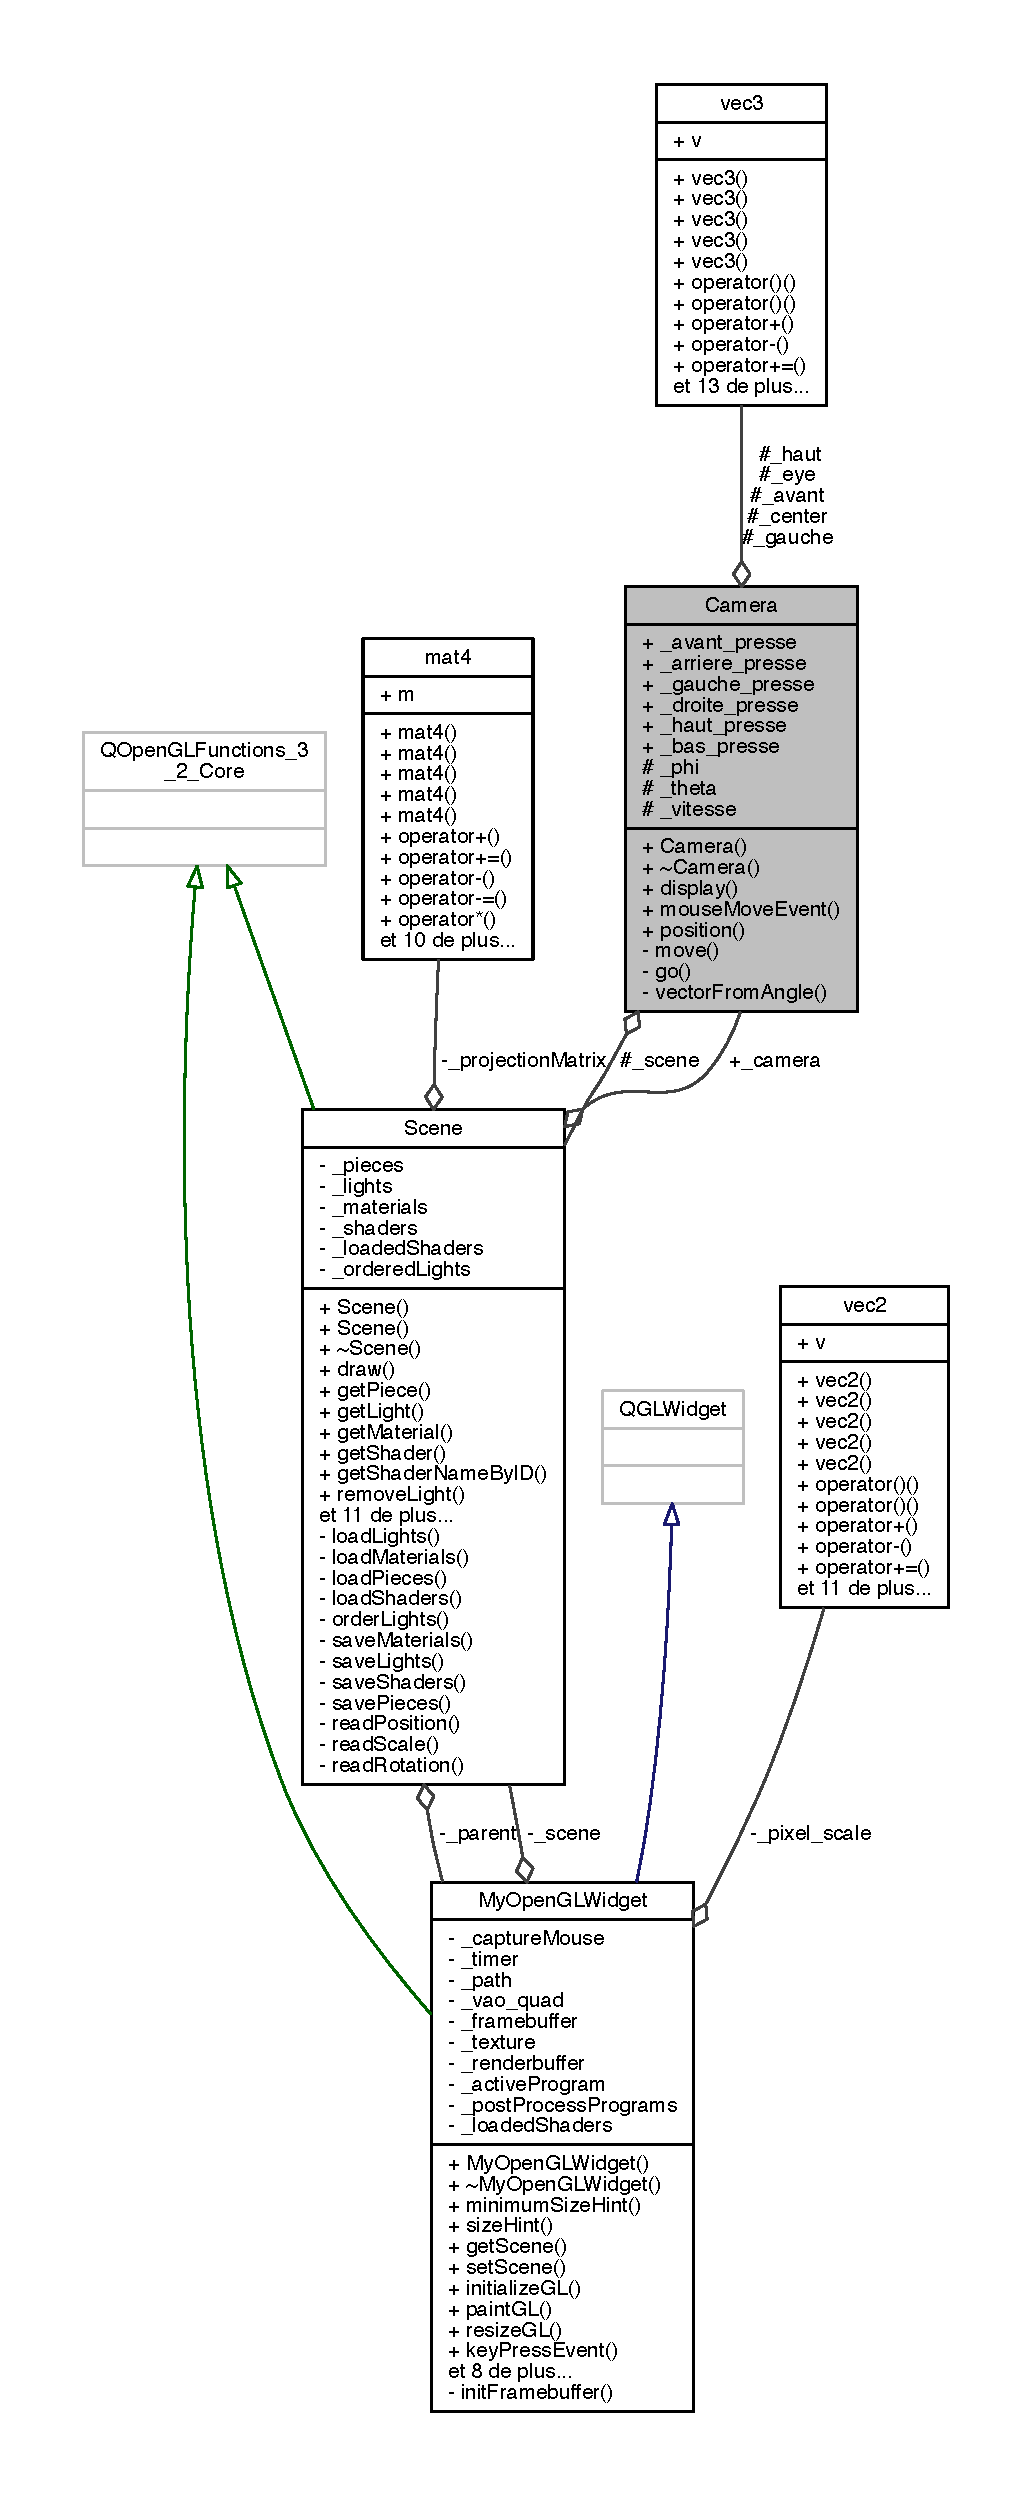
\includegraphics[height=550pt]{class_camera__coll__graph}
\end{center}
\end{figure}
\subsection*{Fonctions membres publiques}
\begin{DoxyCompactItemize}
\item 
\hyperlink{class_camera_a1a8ac754efe577c8abbc1e19cc8bca25}{Camera} (\hyperlink{class_scene}{Scene} $\ast$scene=N\+U\+L\+L, float eye\+X=0.\+0f, float eye\+Y=0.\+0f, float eye\+Z=0.\+0f)
\begin{DoxyCompactList}\small\item\em Constructeur. \end{DoxyCompactList}\item 
\hyperlink{class_camera_ad1897942d0ccf91052386388a497349f}{$\sim$\+Camera} ()
\begin{DoxyCompactList}\small\item\em Destructeur. \end{DoxyCompactList}\item 
void \hyperlink{class_camera_adbfdac30f082ddea86183c1c31493946}{display} ()
\begin{DoxyCompactList}\small\item\em Actualise la caméra. \end{DoxyCompactList}\item 
void \hyperlink{class_camera_a22aaf20b581d402e5c3952655b830c0f}{mouse\+Move\+Event} (int x, int y, int width, int height)
\begin{DoxyCompactList}\small\item\em Fonction de déplacement de la caméra à la souris. \end{DoxyCompactList}\item 
const \hyperlink{structvec3}{vec3} \& \hyperlink{class_camera_ad42b0114b12a48474ae6c8be1c44e7bb}{position} () const 
\begin{DoxyCompactList}\small\item\em Retourne la position de la caméra. \end{DoxyCompactList}\end{DoxyCompactItemize}
\subsection*{Attributs publics}
\begin{DoxyCompactItemize}
\item 
bool \hyperlink{class_camera_a4cab15e35a96fdcb2a8599fea13a9b8f}{\+\_\+avant\+\_\+presse}
\item 
bool \hyperlink{class_camera_a0ce12f74953fcd53192e48f8b4164e2e}{\+\_\+arriere\+\_\+presse}
\item 
bool \hyperlink{class_camera_ac2a5c37c4f9603a14e3616d6a75f7998}{\+\_\+gauche\+\_\+presse}
\item 
bool \hyperlink{class_camera_a61b2e438537b99ba1f0a97e5586b7f45}{\+\_\+droite\+\_\+presse}
\item 
bool \hyperlink{class_camera_a43b59b53cb182906d56e6e4d2c31139c}{\+\_\+haut\+\_\+presse}
\item 
bool \hyperlink{class_camera_aaba6828f97c9ef07b6b135a665bd3008}{\+\_\+bas\+\_\+presse}
\end{DoxyCompactItemize}
\subsection*{Attributs protégés}
\begin{DoxyCompactItemize}
\item 
\hyperlink{structvec3}{vec3} \hyperlink{class_camera_ad4c22c27bd247f4411c4166220ba6e82}{\+\_\+eye}
\item 
\hyperlink{structvec3}{vec3} \hyperlink{class_camera_ad80a82cbc81e6d8ba04c7cc1ac7ba0d7}{\+\_\+center}
\item 
float \hyperlink{class_camera_a288df53a3ff446ee4367ee47b8499fcd}{\+\_\+phi}
\item 
float \hyperlink{class_camera_aeb3c859c3c254c8296420451259e5629}{\+\_\+theta}
\item 
\hyperlink{structvec3}{vec3} \hyperlink{class_camera_ab7cf8c1eae6b2f35a20e8abd1f0570c9}{\+\_\+avant}
\item 
\hyperlink{structvec3}{vec3} \hyperlink{class_camera_aaf97dba7663b99065d8d508b589224de}{\+\_\+gauche}
\item 
\hyperlink{structvec3}{vec3} \hyperlink{class_camera_af860db197a7abbf0284df4e32a95a347}{\+\_\+haut}
\item 
float \hyperlink{class_camera_a9062fdde515a49bf8db963ac46be9942}{\+\_\+vitesse}
\item 
\hyperlink{class_scene}{Scene} $\ast$ \hyperlink{class_camera_a81ffb00eedbaefbfb755b0c13d42180a}{\+\_\+scene}
\end{DoxyCompactItemize}
\subsection*{Fonctions membres privées}
\begin{DoxyCompactItemize}
\item 
void \hyperlink{class_camera_a8414e6d74d3f6259fa5ea1f037e9d8bd}{move} ()
\begin{DoxyCompactList}\small\item\em Calcul le déplacement de la \hyperlink{class_camera}{Camera}. \end{DoxyCompactList}\item 
void \hyperlink{class_camera_abde0ff477fb0baea7515767dcd7a7cf7}{go} (float x, float y, float z)
\begin{DoxyCompactList}\small\item\em Déplace la caméra aux coordonnées données. \end{DoxyCompactList}\item 
void \hyperlink{class_camera_aa4e815462a964caa6b10804e33119cf2}{vector\+From\+Angle} ()
\begin{DoxyCompactList}\small\item\em Recalcul les vecteurs avant/côté pour le mouvement. \end{DoxyCompactList}\end{DoxyCompactItemize}


\subsection{Description détaillée}
\hyperlink{class_camera}{Camera} pour \hyperlink{class_scene}{Scene}. 

\subsection{Documentation des constructeurs et destructeur}
\hypertarget{class_camera_a1a8ac754efe577c8abbc1e19cc8bca25}{\index{Camera@{Camera}!Camera@{Camera}}
\index{Camera@{Camera}!Camera@{Camera}}
\subsubsection[{Camera}]{\setlength{\rightskip}{0pt plus 5cm}Camera\+::\+Camera (
\begin{DoxyParamCaption}
\item[{{\bf Scene} $\ast$}]{scene = {\ttfamily NULL}, }
\item[{float}]{eye\+X = {\ttfamily 0.0f}, }
\item[{float}]{eye\+Y = {\ttfamily 0.0f}, }
\item[{float}]{eye\+Z = {\ttfamily 0.0f}}
\end{DoxyParamCaption}
)}}\label{class_camera_a1a8ac754efe577c8abbc1e19cc8bca25}


Constructeur. 



Voici le graphe d'appel pour cette fonction \+:
\nopagebreak
\begin{figure}[H]
\begin{center}
\leavevmode
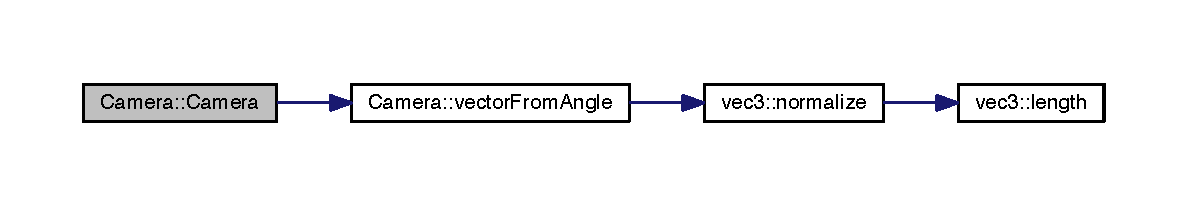
\includegraphics[width=350pt]{class_camera_a1a8ac754efe577c8abbc1e19cc8bca25_cgraph}
\end{center}
\end{figure}


\hypertarget{class_camera_ad1897942d0ccf91052386388a497349f}{\index{Camera@{Camera}!````~Camera@{$\sim$\+Camera}}
\index{````~Camera@{$\sim$\+Camera}!Camera@{Camera}}
\subsubsection[{$\sim$\+Camera}]{\setlength{\rightskip}{0pt plus 5cm}Camera\+::$\sim$\+Camera (
\begin{DoxyParamCaption}
{}
\end{DoxyParamCaption}
)\hspace{0.3cm}{\ttfamily [inline]}}}\label{class_camera_ad1897942d0ccf91052386388a497349f}


Destructeur. 



\subsection{Documentation des fonctions membres}
\hypertarget{class_camera_adbfdac30f082ddea86183c1c31493946}{\index{Camera@{Camera}!display@{display}}
\index{display@{display}!Camera@{Camera}}
\subsubsection[{display}]{\setlength{\rightskip}{0pt plus 5cm}void Camera\+::display (
\begin{DoxyParamCaption}
{}
\end{DoxyParamCaption}
)}}\label{class_camera_adbfdac30f082ddea86183c1c31493946}


Actualise la caméra. 

Met à jour la position de la caméra en fonction des booléens de déplacement et actualise la matrice view 

Voici le graphe d'appel pour cette fonction \+:
\nopagebreak
\begin{figure}[H]
\begin{center}
\leavevmode
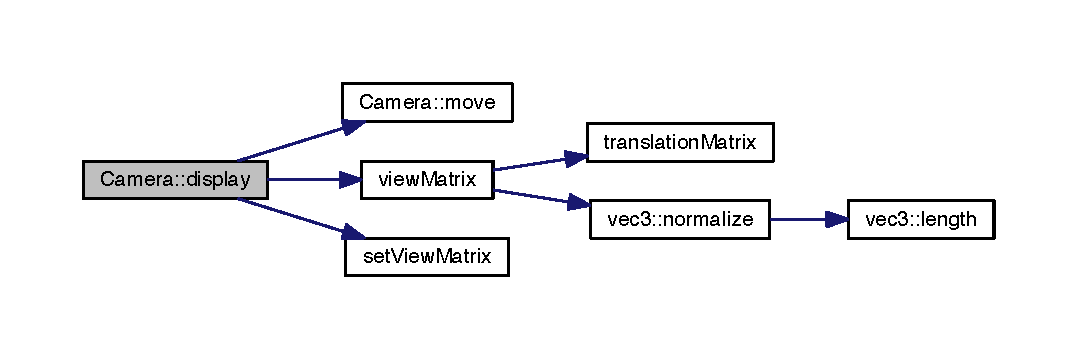
\includegraphics[width=350pt]{class_camera_adbfdac30f082ddea86183c1c31493946_cgraph}
\end{center}
\end{figure}




Voici le graphe des appelants de cette fonction \+:
\nopagebreak
\begin{figure}[H]
\begin{center}
\leavevmode
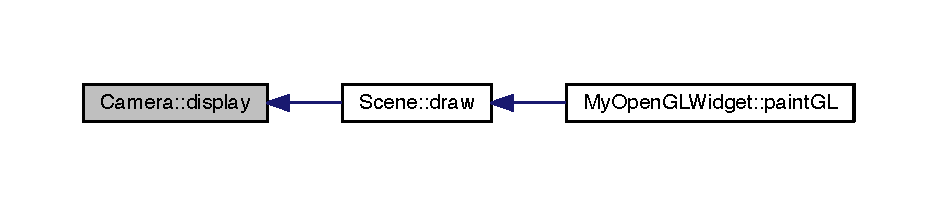
\includegraphics[width=350pt]{class_camera_adbfdac30f082ddea86183c1c31493946_icgraph}
\end{center}
\end{figure}


\hypertarget{class_camera_abde0ff477fb0baea7515767dcd7a7cf7}{\index{Camera@{Camera}!go@{go}}
\index{go@{go}!Camera@{Camera}}
\subsubsection[{go}]{\setlength{\rightskip}{0pt plus 5cm}void Camera\+::go (
\begin{DoxyParamCaption}
\item[{float}]{x, }
\item[{float}]{y, }
\item[{float}]{z}
\end{DoxyParamCaption}
)\hspace{0.3cm}{\ttfamily [private]}}}\label{class_camera_abde0ff477fb0baea7515767dcd7a7cf7}


Déplace la caméra aux coordonnées données. 

\hypertarget{class_camera_a22aaf20b581d402e5c3952655b830c0f}{\index{Camera@{Camera}!mouse\+Move\+Event@{mouse\+Move\+Event}}
\index{mouse\+Move\+Event@{mouse\+Move\+Event}!Camera@{Camera}}
\subsubsection[{mouse\+Move\+Event}]{\setlength{\rightskip}{0pt plus 5cm}void Camera\+::mouse\+Move\+Event (
\begin{DoxyParamCaption}
\item[{int}]{x, }
\item[{int}]{y, }
\item[{int}]{width, }
\item[{int}]{height}
\end{DoxyParamCaption}
)}}\label{class_camera_a22aaf20b581d402e5c3952655b830c0f}


Fonction de déplacement de la caméra à la souris. 


\begin{DoxyParams}{Paramètres}
{\em x} & position en X du curseur de la souris \\
\hline
{\em y} & position en Y du curseur de la souris \\
\hline
{\em width} & largeur de la fenêtre \\
\hline
{\em height} & hauteur de la fenêtre \\
\hline
\end{DoxyParams}


Voici le graphe d'appel pour cette fonction \+:
\nopagebreak
\begin{figure}[H]
\begin{center}
\leavevmode
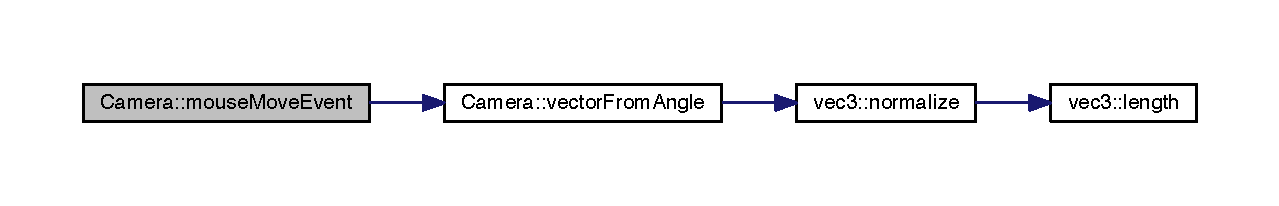
\includegraphics[width=350pt]{class_camera_a22aaf20b581d402e5c3952655b830c0f_cgraph}
\end{center}
\end{figure}




Voici le graphe des appelants de cette fonction \+:
\nopagebreak
\begin{figure}[H]
\begin{center}
\leavevmode
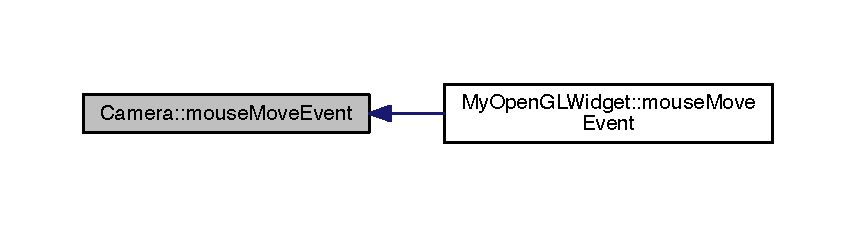
\includegraphics[width=350pt]{class_camera_a22aaf20b581d402e5c3952655b830c0f_icgraph}
\end{center}
\end{figure}


\hypertarget{class_camera_a8414e6d74d3f6259fa5ea1f037e9d8bd}{\index{Camera@{Camera}!move@{move}}
\index{move@{move}!Camera@{Camera}}
\subsubsection[{move}]{\setlength{\rightskip}{0pt plus 5cm}void Camera\+::move (
\begin{DoxyParamCaption}
{}
\end{DoxyParamCaption}
)\hspace{0.3cm}{\ttfamily [private]}}}\label{class_camera_a8414e6d74d3f6259fa5ea1f037e9d8bd}


Calcul le déplacement de la \hyperlink{class_camera}{Camera}. 



Voici le graphe des appelants de cette fonction \+:
\nopagebreak
\begin{figure}[H]
\begin{center}
\leavevmode
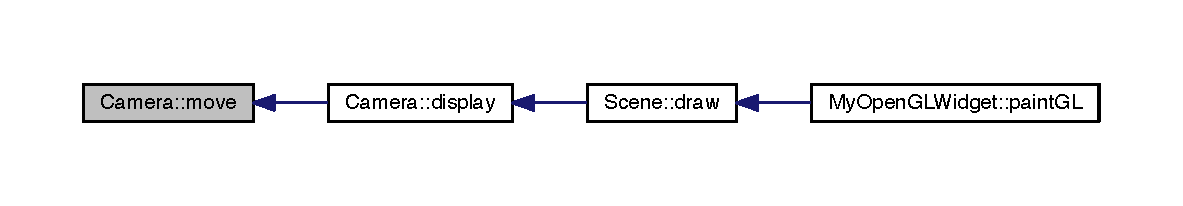
\includegraphics[width=350pt]{class_camera_a8414e6d74d3f6259fa5ea1f037e9d8bd_icgraph}
\end{center}
\end{figure}


\hypertarget{class_camera_ad42b0114b12a48474ae6c8be1c44e7bb}{\index{Camera@{Camera}!position@{position}}
\index{position@{position}!Camera@{Camera}}
\subsubsection[{position}]{\setlength{\rightskip}{0pt plus 5cm}const {\bf vec3}\& Camera\+::position (
\begin{DoxyParamCaption}
{}
\end{DoxyParamCaption}
) const\hspace{0.3cm}{\ttfamily [inline]}}}\label{class_camera_ad42b0114b12a48474ae6c8be1c44e7bb}


Retourne la position de la caméra. 



Voici le graphe des appelants de cette fonction \+:
\nopagebreak
\begin{figure}[H]
\begin{center}
\leavevmode
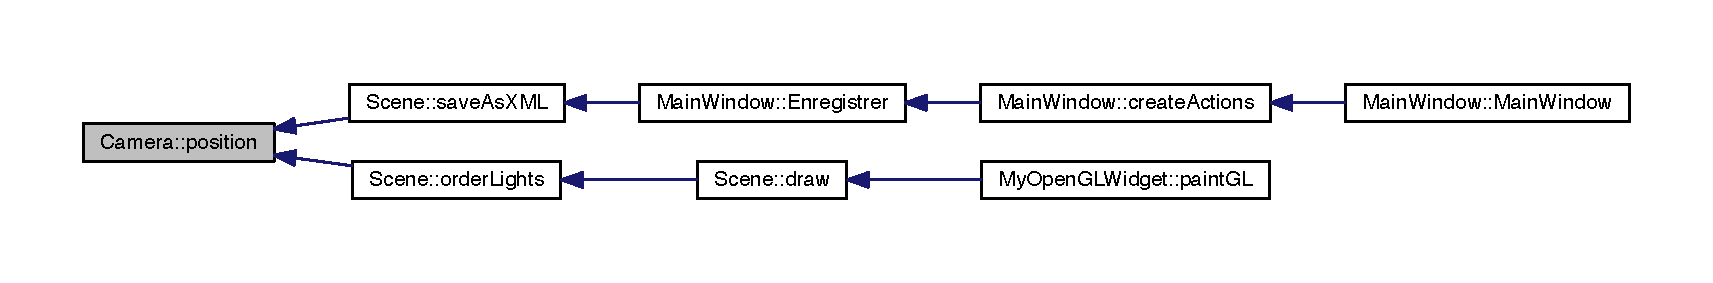
\includegraphics[width=350pt]{class_camera_ad42b0114b12a48474ae6c8be1c44e7bb_icgraph}
\end{center}
\end{figure}


\hypertarget{class_camera_aa4e815462a964caa6b10804e33119cf2}{\index{Camera@{Camera}!vector\+From\+Angle@{vector\+From\+Angle}}
\index{vector\+From\+Angle@{vector\+From\+Angle}!Camera@{Camera}}
\subsubsection[{vector\+From\+Angle}]{\setlength{\rightskip}{0pt plus 5cm}void Camera\+::vector\+From\+Angle (
\begin{DoxyParamCaption}
{}
\end{DoxyParamCaption}
)\hspace{0.3cm}{\ttfamily [private]}}}\label{class_camera_aa4e815462a964caa6b10804e33119cf2}


Recalcul les vecteurs avant/côté pour le mouvement. 



Voici le graphe d'appel pour cette fonction \+:
\nopagebreak
\begin{figure}[H]
\begin{center}
\leavevmode
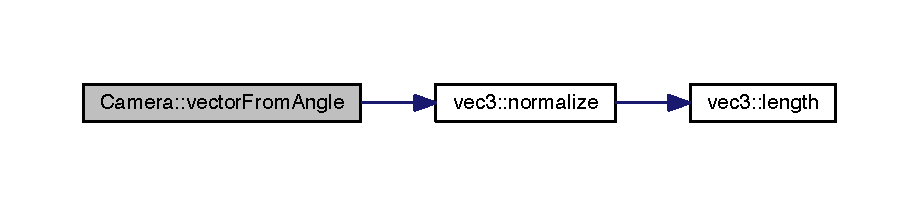
\includegraphics[width=350pt]{class_camera_aa4e815462a964caa6b10804e33119cf2_cgraph}
\end{center}
\end{figure}




Voici le graphe des appelants de cette fonction \+:
\nopagebreak
\begin{figure}[H]
\begin{center}
\leavevmode
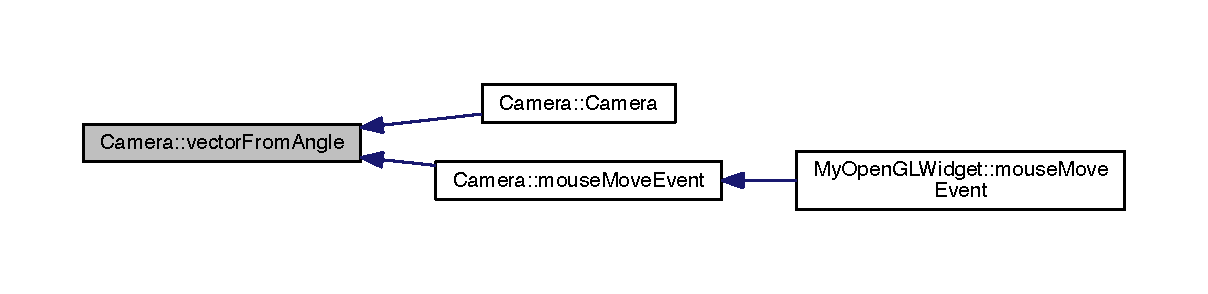
\includegraphics[width=350pt]{class_camera_aa4e815462a964caa6b10804e33119cf2_icgraph}
\end{center}
\end{figure}




\subsection{Documentation des données membres}
\hypertarget{class_camera_a0ce12f74953fcd53192e48f8b4164e2e}{\index{Camera@{Camera}!\+\_\+arriere\+\_\+presse@{\+\_\+arriere\+\_\+presse}}
\index{\+\_\+arriere\+\_\+presse@{\+\_\+arriere\+\_\+presse}!Camera@{Camera}}
\subsubsection[{\+\_\+arriere\+\_\+presse}]{\setlength{\rightskip}{0pt plus 5cm}bool Camera\+::\+\_\+arriere\+\_\+presse}}\label{class_camera_a0ce12f74953fcd53192e48f8b4164e2e}
Indique si la caméra doit reculer au prochain affichage \hypertarget{class_camera_ab7cf8c1eae6b2f35a20e8abd1f0570c9}{\index{Camera@{Camera}!\+\_\+avant@{\+\_\+avant}}
\index{\+\_\+avant@{\+\_\+avant}!Camera@{Camera}}
\subsubsection[{\+\_\+avant}]{\setlength{\rightskip}{0pt plus 5cm}{\bf vec3} Camera\+::\+\_\+avant\hspace{0.3cm}{\ttfamily [protected]}}}\label{class_camera_ab7cf8c1eae6b2f35a20e8abd1f0570c9}
\hypertarget{class_camera_a4cab15e35a96fdcb2a8599fea13a9b8f}{\index{Camera@{Camera}!\+\_\+avant\+\_\+presse@{\+\_\+avant\+\_\+presse}}
\index{\+\_\+avant\+\_\+presse@{\+\_\+avant\+\_\+presse}!Camera@{Camera}}
\subsubsection[{\+\_\+avant\+\_\+presse}]{\setlength{\rightskip}{0pt plus 5cm}bool Camera\+::\+\_\+avant\+\_\+presse}}\label{class_camera_a4cab15e35a96fdcb2a8599fea13a9b8f}
Indique si la caméra doit avancer au prochain affichage \hypertarget{class_camera_aaba6828f97c9ef07b6b135a665bd3008}{\index{Camera@{Camera}!\+\_\+bas\+\_\+presse@{\+\_\+bas\+\_\+presse}}
\index{\+\_\+bas\+\_\+presse@{\+\_\+bas\+\_\+presse}!Camera@{Camera}}
\subsubsection[{\+\_\+bas\+\_\+presse}]{\setlength{\rightskip}{0pt plus 5cm}bool Camera\+::\+\_\+bas\+\_\+presse}}\label{class_camera_aaba6828f97c9ef07b6b135a665bd3008}
Indique si la caméra doit descendre au prochain affichage \hypertarget{class_camera_ad80a82cbc81e6d8ba04c7cc1ac7ba0d7}{\index{Camera@{Camera}!\+\_\+center@{\+\_\+center}}
\index{\+\_\+center@{\+\_\+center}!Camera@{Camera}}
\subsubsection[{\+\_\+center}]{\setlength{\rightskip}{0pt plus 5cm}{\bf vec3} Camera\+::\+\_\+center\hspace{0.3cm}{\ttfamily [protected]}}}\label{class_camera_ad80a82cbc81e6d8ba04c7cc1ac7ba0d7}
\hypertarget{class_camera_a61b2e438537b99ba1f0a97e5586b7f45}{\index{Camera@{Camera}!\+\_\+droite\+\_\+presse@{\+\_\+droite\+\_\+presse}}
\index{\+\_\+droite\+\_\+presse@{\+\_\+droite\+\_\+presse}!Camera@{Camera}}
\subsubsection[{\+\_\+droite\+\_\+presse}]{\setlength{\rightskip}{0pt plus 5cm}bool Camera\+::\+\_\+droite\+\_\+presse}}\label{class_camera_a61b2e438537b99ba1f0a97e5586b7f45}
Indique si la caméra doit aller à droite au prochain affichage \hypertarget{class_camera_ad4c22c27bd247f4411c4166220ba6e82}{\index{Camera@{Camera}!\+\_\+eye@{\+\_\+eye}}
\index{\+\_\+eye@{\+\_\+eye}!Camera@{Camera}}
\subsubsection[{\+\_\+eye}]{\setlength{\rightskip}{0pt plus 5cm}{\bf vec3} Camera\+::\+\_\+eye\hspace{0.3cm}{\ttfamily [protected]}}}\label{class_camera_ad4c22c27bd247f4411c4166220ba6e82}
\hypertarget{class_camera_aaf97dba7663b99065d8d508b589224de}{\index{Camera@{Camera}!\+\_\+gauche@{\+\_\+gauche}}
\index{\+\_\+gauche@{\+\_\+gauche}!Camera@{Camera}}
\subsubsection[{\+\_\+gauche}]{\setlength{\rightskip}{0pt plus 5cm}{\bf vec3} Camera\+::\+\_\+gauche\hspace{0.3cm}{\ttfamily [protected]}}}\label{class_camera_aaf97dba7663b99065d8d508b589224de}
\hypertarget{class_camera_ac2a5c37c4f9603a14e3616d6a75f7998}{\index{Camera@{Camera}!\+\_\+gauche\+\_\+presse@{\+\_\+gauche\+\_\+presse}}
\index{\+\_\+gauche\+\_\+presse@{\+\_\+gauche\+\_\+presse}!Camera@{Camera}}
\subsubsection[{\+\_\+gauche\+\_\+presse}]{\setlength{\rightskip}{0pt plus 5cm}bool Camera\+::\+\_\+gauche\+\_\+presse}}\label{class_camera_ac2a5c37c4f9603a14e3616d6a75f7998}
Indique si la caméra doit aller à gauche au prochain affichage \hypertarget{class_camera_af860db197a7abbf0284df4e32a95a347}{\index{Camera@{Camera}!\+\_\+haut@{\+\_\+haut}}
\index{\+\_\+haut@{\+\_\+haut}!Camera@{Camera}}
\subsubsection[{\+\_\+haut}]{\setlength{\rightskip}{0pt plus 5cm}{\bf vec3} Camera\+::\+\_\+haut\hspace{0.3cm}{\ttfamily [protected]}}}\label{class_camera_af860db197a7abbf0284df4e32a95a347}
\hypertarget{class_camera_a43b59b53cb182906d56e6e4d2c31139c}{\index{Camera@{Camera}!\+\_\+haut\+\_\+presse@{\+\_\+haut\+\_\+presse}}
\index{\+\_\+haut\+\_\+presse@{\+\_\+haut\+\_\+presse}!Camera@{Camera}}
\subsubsection[{\+\_\+haut\+\_\+presse}]{\setlength{\rightskip}{0pt plus 5cm}bool Camera\+::\+\_\+haut\+\_\+presse}}\label{class_camera_a43b59b53cb182906d56e6e4d2c31139c}
Indique si la caméra doit monter au prochain affichage \hypertarget{class_camera_a288df53a3ff446ee4367ee47b8499fcd}{\index{Camera@{Camera}!\+\_\+phi@{\+\_\+phi}}
\index{\+\_\+phi@{\+\_\+phi}!Camera@{Camera}}
\subsubsection[{\+\_\+phi}]{\setlength{\rightskip}{0pt plus 5cm}float Camera\+::\+\_\+phi\hspace{0.3cm}{\ttfamily [protected]}}}\label{class_camera_a288df53a3ff446ee4367ee47b8499fcd}
\hypertarget{class_camera_a81ffb00eedbaefbfb755b0c13d42180a}{\index{Camera@{Camera}!\+\_\+scene@{\+\_\+scene}}
\index{\+\_\+scene@{\+\_\+scene}!Camera@{Camera}}
\subsubsection[{\+\_\+scene}]{\setlength{\rightskip}{0pt plus 5cm}{\bf Scene}$\ast$ Camera\+::\+\_\+scene\hspace{0.3cm}{\ttfamily [protected]}}}\label{class_camera_a81ffb00eedbaefbfb755b0c13d42180a}
\hypertarget{class_camera_aeb3c859c3c254c8296420451259e5629}{\index{Camera@{Camera}!\+\_\+theta@{\+\_\+theta}}
\index{\+\_\+theta@{\+\_\+theta}!Camera@{Camera}}
\subsubsection[{\+\_\+theta}]{\setlength{\rightskip}{0pt plus 5cm}float Camera\+::\+\_\+theta\hspace{0.3cm}{\ttfamily [protected]}}}\label{class_camera_aeb3c859c3c254c8296420451259e5629}
\hypertarget{class_camera_a9062fdde515a49bf8db963ac46be9942}{\index{Camera@{Camera}!\+\_\+vitesse@{\+\_\+vitesse}}
\index{\+\_\+vitesse@{\+\_\+vitesse}!Camera@{Camera}}
\subsubsection[{\+\_\+vitesse}]{\setlength{\rightskip}{0pt plus 5cm}float Camera\+::\+\_\+vitesse\hspace{0.3cm}{\ttfamily [protected]}}}\label{class_camera_a9062fdde515a49bf8db963ac46be9942}


La documentation de cette classe a été générée à partir des fichiers suivants \+:\begin{DoxyCompactItemize}
\item 
\hyperlink{camera_8hpp}{camera.\+hpp}\item 
\hyperlink{camera_8cpp}{camera.\+cpp}\end{DoxyCompactItemize}

\hypertarget{class_cube}{\section{Référence de la classe Cube}
\label{class_cube}\index{Cube@{Cube}}
}


Primitive cube.  




{\ttfamily \#include $<$cube.\+hpp$>$}



Graphe d'héritage de Cube\+:
\nopagebreak
\begin{figure}[H]
\begin{center}
\leavevmode
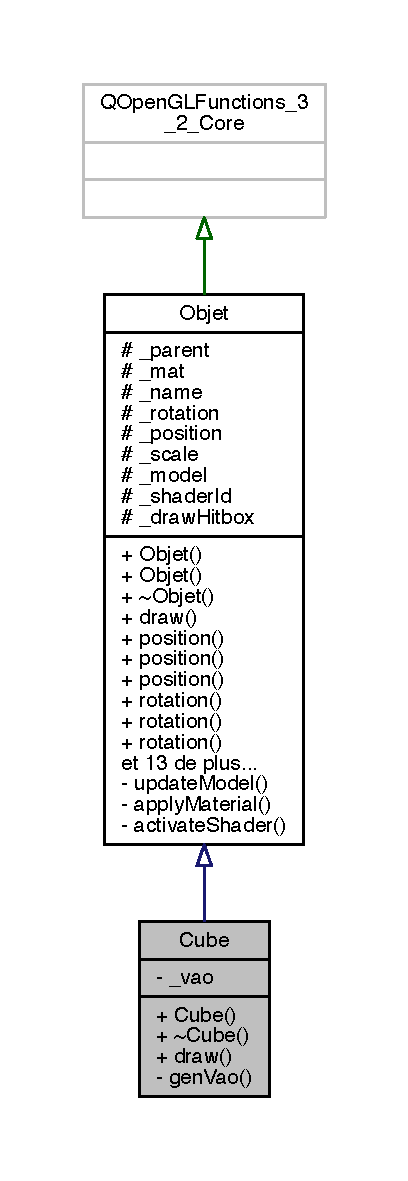
\includegraphics[height=550pt]{class_cube__inherit__graph}
\end{center}
\end{figure}


Graphe de collaboration de Cube\+:
\nopagebreak
\begin{figure}[H]
\begin{center}
\leavevmode
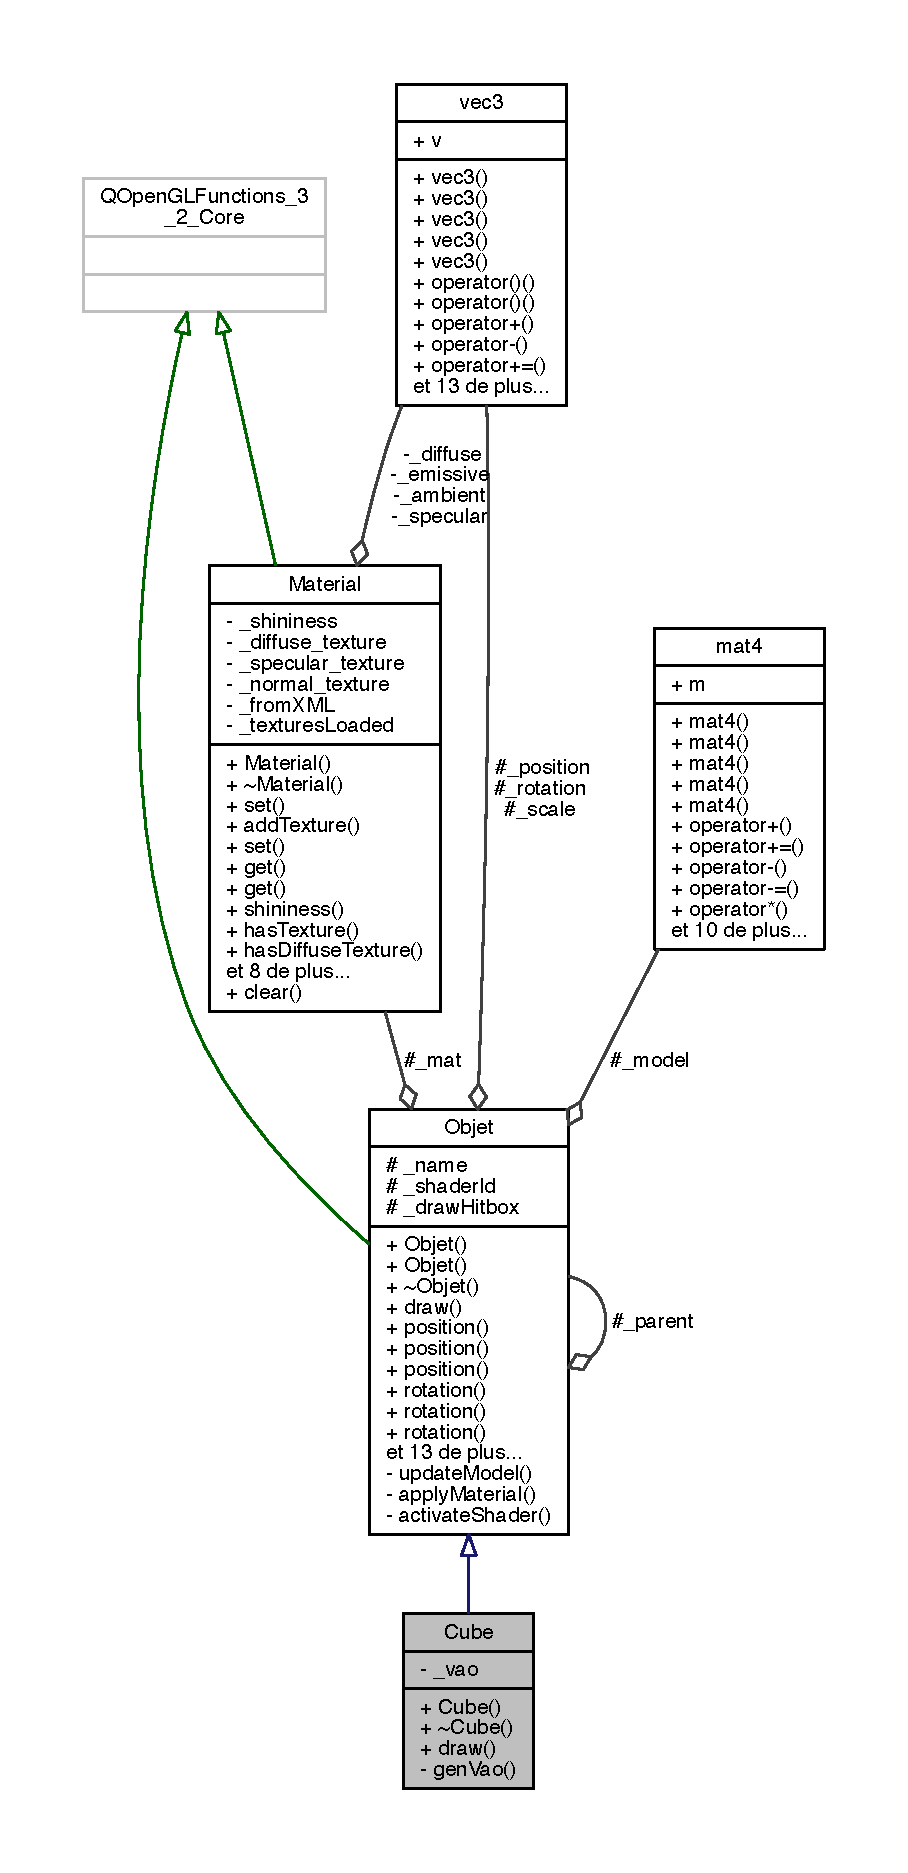
\includegraphics[height=550pt]{class_cube__coll__graph}
\end{center}
\end{figure}
\subsection*{Fonctions membres publiques}
\begin{DoxyCompactItemize}
\item 
\hyperlink{class_cube_a6d016e01f3fee45cff97be27ff7175d8}{Cube} (\hyperlink{class_material}{Material} $\ast$mat=N\+U\+L\+L, \hyperlink{structvec3}{vec3} \hyperlink{class_objet_ac69a1b459bcb4433099c8cfbff06b209}{rotation}=\hyperlink{structvec3}{vec3}(), \hyperlink{structvec3}{vec3} \hyperlink{class_objet_a0e109bc790b14328202dd2546b04e2fd}{position}=\hyperlink{structvec3}{vec3}())
\begin{DoxyCompactList}\small\item\em Constructeur du cube. \end{DoxyCompactList}\item 
\hyperlink{class_cube_aa814e979cecb8c451fdb332ded2cea1e}{$\sim$\+Cube} ()
\begin{DoxyCompactList}\small\item\em Destructeur du cube. \end{DoxyCompactList}\item 
void \hyperlink{class_cube_ab26b72a81376fd5dc4fcc7f0b715b087}{draw} ()
\begin{DoxyCompactList}\small\item\em Affiche le cube. \end{DoxyCompactList}\end{DoxyCompactItemize}
\subsection*{Fonctions membres privées}
\begin{DoxyCompactItemize}
\item 
void \hyperlink{class_cube_a06f4c8632c223f8d8c34971e55a2dafc}{gen\+Vao} ()
\begin{DoxyCompactList}\small\item\em Génère les vbo et le vao pour l'affichage du cube. \end{DoxyCompactList}\end{DoxyCompactItemize}
\subsection*{Attributs privés statiques}
\begin{DoxyCompactItemize}
\item 
static G\+Luint \hyperlink{class_cube_ae474ca8293842dd9ac83a8c606991eac}{\+\_\+vao} = 0
\end{DoxyCompactItemize}
\subsection*{Membres hérités additionnels}


\subsection{Description détaillée}
Primitive cube. 

\begin{DoxyWarning}{Avertissement}
Peut être plus utilisable 
\end{DoxyWarning}


\subsection{Documentation des constructeurs et destructeur}
\hypertarget{class_cube_a6d016e01f3fee45cff97be27ff7175d8}{\index{Cube@{Cube}!Cube@{Cube}}
\index{Cube@{Cube}!Cube@{Cube}}
\subsubsection[{Cube}]{\setlength{\rightskip}{0pt plus 5cm}Cube\+::\+Cube (
\begin{DoxyParamCaption}
\item[{{\bf Material} $\ast$}]{mat = {\ttfamily NULL}, }
\item[{{\bf vec3}}]{rotation = {\ttfamily {\bf vec3}()}, }
\item[{{\bf vec3}}]{position = {\ttfamily {\bf vec3}()}}
\end{DoxyParamCaption}
)}}\label{class_cube_a6d016e01f3fee45cff97be27ff7175d8}


Constructeur du cube. 

Génère le vao et les vbo s'ils n'ont pas déjà été générés 

Voici le graphe d'appel pour cette fonction \+:
\nopagebreak
\begin{figure}[H]
\begin{center}
\leavevmode
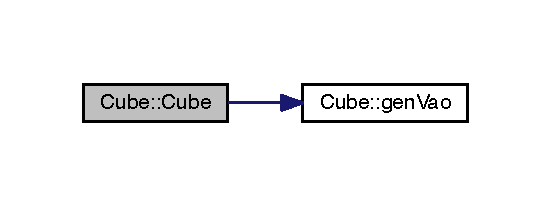
\includegraphics[width=265pt]{class_cube_a6d016e01f3fee45cff97be27ff7175d8_cgraph}
\end{center}
\end{figure}


\hypertarget{class_cube_aa814e979cecb8c451fdb332ded2cea1e}{\index{Cube@{Cube}!````~Cube@{$\sim$\+Cube}}
\index{````~Cube@{$\sim$\+Cube}!Cube@{Cube}}
\subsubsection[{$\sim$\+Cube}]{\setlength{\rightskip}{0pt plus 5cm}Cube\+::$\sim$\+Cube (
\begin{DoxyParamCaption}
{}
\end{DoxyParamCaption}
)}}\label{class_cube_aa814e979cecb8c451fdb332ded2cea1e}


Destructeur du cube. 



\subsection{Documentation des fonctions membres}
\hypertarget{class_cube_ab26b72a81376fd5dc4fcc7f0b715b087}{\index{Cube@{Cube}!draw@{draw}}
\index{draw@{draw}!Cube@{Cube}}
\subsubsection[{draw}]{\setlength{\rightskip}{0pt plus 5cm}void Cube\+::draw (
\begin{DoxyParamCaption}
{}
\end{DoxyParamCaption}
)\hspace{0.3cm}{\ttfamily [virtual]}}}\label{class_cube_ab26b72a81376fd5dc4fcc7f0b715b087}


Affiche le cube. 



Réimplémentée à partir de \hyperlink{class_objet_a5cc323f562964e00b947b2d908e206e7}{Objet}.



Voici le graphe d'appel pour cette fonction \+:
\nopagebreak
\begin{figure}[H]
\begin{center}
\leavevmode
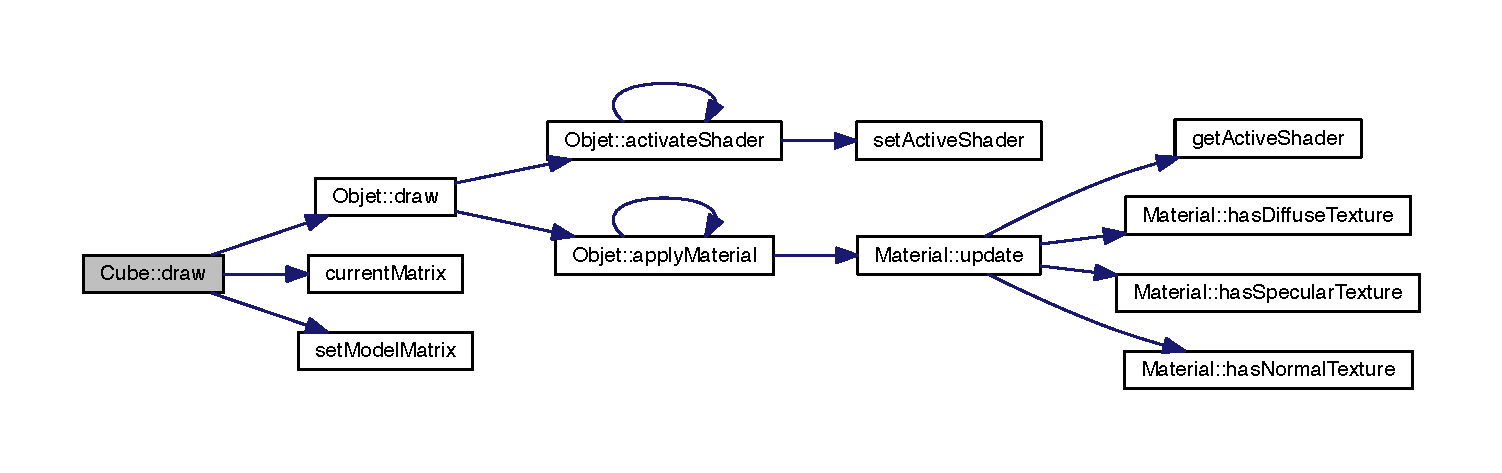
\includegraphics[width=350pt]{class_cube_ab26b72a81376fd5dc4fcc7f0b715b087_cgraph}
\end{center}
\end{figure}


\hypertarget{class_cube_a06f4c8632c223f8d8c34971e55a2dafc}{\index{Cube@{Cube}!gen\+Vao@{gen\+Vao}}
\index{gen\+Vao@{gen\+Vao}!Cube@{Cube}}
\subsubsection[{gen\+Vao}]{\setlength{\rightskip}{0pt plus 5cm}void Cube\+::gen\+Vao (
\begin{DoxyParamCaption}
{}
\end{DoxyParamCaption}
)\hspace{0.3cm}{\ttfamily [private]}}}\label{class_cube_a06f4c8632c223f8d8c34971e55a2dafc}


Génère les vbo et le vao pour l'affichage du cube. 



Voici le graphe des appelants de cette fonction \+:
\nopagebreak
\begin{figure}[H]
\begin{center}
\leavevmode
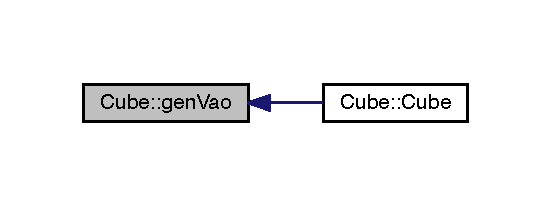
\includegraphics[width=265pt]{class_cube_a06f4c8632c223f8d8c34971e55a2dafc_icgraph}
\end{center}
\end{figure}




\subsection{Documentation des données membres}
\hypertarget{class_cube_ae474ca8293842dd9ac83a8c606991eac}{\index{Cube@{Cube}!\+\_\+vao@{\+\_\+vao}}
\index{\+\_\+vao@{\+\_\+vao}!Cube@{Cube}}
\subsubsection[{\+\_\+vao}]{\setlength{\rightskip}{0pt plus 5cm}G\+Luint Cube\+::\+\_\+vao = 0\hspace{0.3cm}{\ttfamily [static]}, {\ttfamily [private]}}}\label{class_cube_ae474ca8293842dd9ac83a8c606991eac}
$<$ Id du Vao du cube 

La documentation de cette classe a été générée à partir des fichiers suivants \+:\begin{DoxyCompactItemize}
\item 
objets/\hyperlink{cube_8hpp}{cube.\+hpp}\item 
objets/\hyperlink{cube_8cpp}{cube.\+cpp}\end{DoxyCompactItemize}

\hypertarget{class_donuts}{\section{Donuts Class Reference}
\label{class_donuts}\index{Donuts@{Donuts}}
}


Primitive tore.  




{\ttfamily \#include $<$donuts.\+hpp$>$}

Inheritance diagram for Donuts\+:\begin{figure}[H]
\begin{center}
\leavevmode
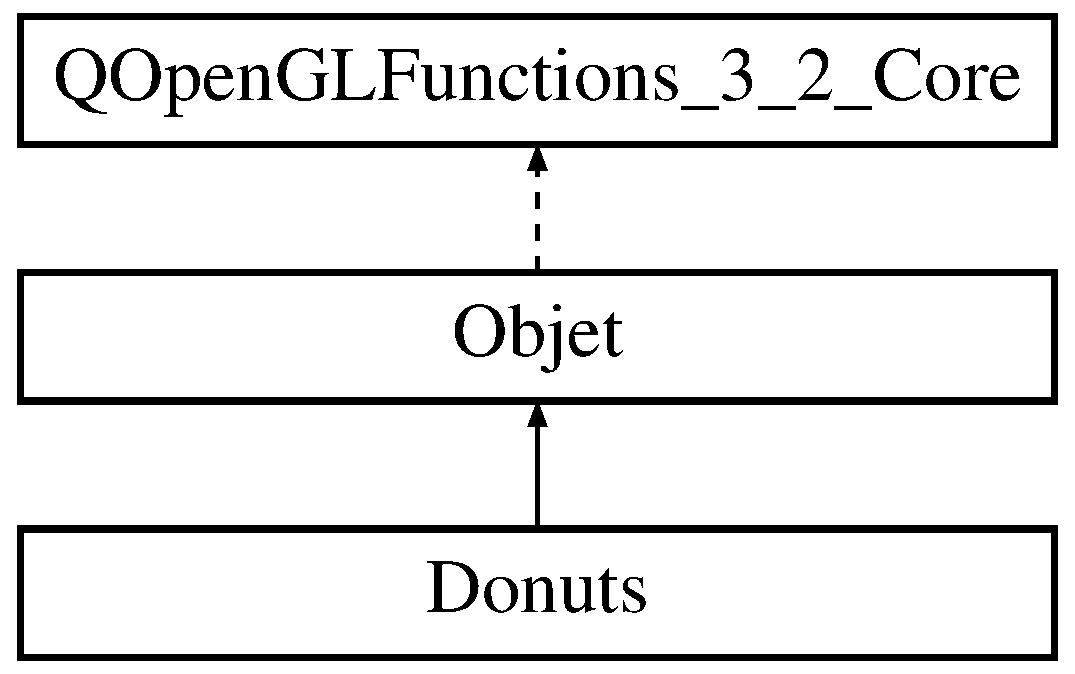
\includegraphics[height=3.000000cm]{class_donuts}
\end{center}
\end{figure}
\subsection*{Public Member Functions}
\begin{DoxyCompactItemize}
\item 
\hyperlink{class_donuts_a91d8d9b011ed1f7e406a2906f2b6e898}{Donuts} (G\+Ldouble \hyperlink{class_donuts_ae3db8d4ea17228ed43d388bac7fb35b3}{m\+\_\+radius}=1, G\+Ldouble \hyperlink{class_donuts_a5050c790a74b5313a06b818a7f3e8723}{m\+\_\+radius\+\_\+donuts}=1, G\+Lint \hyperlink{class_donuts_a2214ac47effb92c5de33fa7c57d28694}{m\+\_\+slices}=1, G\+Lint \hyperlink{class_donuts_a5273bc3a4bdada5e4302b35d49bdd550}{m\+\_\+stacks}=1, \hyperlink{class_material}{Material} $\ast$mat=N\+U\+L\+L, \hyperlink{structvec3}{vec3} \hyperlink{class_objet_ac69a1b459bcb4433099c8cfbff06b209}{rotation}=\hyperlink{structvec3}{vec3}(), \hyperlink{structvec3}{vec3} \hyperlink{class_objet_a0e109bc790b14328202dd2546b04e2fd}{position}=\hyperlink{structvec3}{vec3}())
\item 
\hyperlink{class_donuts_aea6536802eeb29b4fa4eee2f7e1ea626}{$\sim$\+Donuts} ()
\item 
void \hyperlink{class_donuts_a5a7932c8494905ba09bb515a01e6c91d}{draw} ()
\begin{DoxyCompactList}\small\item\em Affichage de l'\hyperlink{class_objet}{Objet}. \end{DoxyCompactList}\end{DoxyCompactItemize}
\subsection*{Private Member Functions}
\begin{DoxyCompactItemize}
\item 
void \hyperlink{class_donuts_aff7950429cf43ee2898c6f1a6545b174}{gen\+Vao} ()
\end{DoxyCompactItemize}
\subsection*{Private Attributes}
\begin{DoxyCompactItemize}
\item 
G\+Luint \hyperlink{class_donuts_a659c70b043ddc2ebcdc64bcb58c1e621}{\+\_\+vao}
\item 
G\+Ldouble \hyperlink{class_donuts_ae3db8d4ea17228ed43d388bac7fb35b3}{m\+\_\+radius}
\item 
G\+Ldouble \hyperlink{class_donuts_a5050c790a74b5313a06b818a7f3e8723}{m\+\_\+radius\+\_\+donuts}
\item 
G\+Lint \hyperlink{class_donuts_a2214ac47effb92c5de33fa7c57d28694}{m\+\_\+slices}
\item 
G\+Lint \hyperlink{class_donuts_a5273bc3a4bdada5e4302b35d49bdd550}{m\+\_\+stacks}
\item 
G\+Lsizei \hyperlink{class_donuts_aac0118d276a512d287a9bc1f4c7d249d}{nbvertex}
\end{DoxyCompactItemize}
\subsection*{Additional Inherited Members}


\subsection{Detailed Description}
Primitive tore. 

\begin{DoxyWarning}{Warning}
Peut être plus utilisable 
\end{DoxyWarning}
\begin{DoxySeeAlso}{See also}
\hyperlink{class_cube}{Cube} 
\end{DoxySeeAlso}


\subsection{Constructor \& Destructor Documentation}
\hypertarget{class_donuts_a91d8d9b011ed1f7e406a2906f2b6e898}{\index{Donuts@{Donuts}!Donuts@{Donuts}}
\index{Donuts@{Donuts}!Donuts@{Donuts}}
\subsubsection[{Donuts}]{\setlength{\rightskip}{0pt plus 5cm}Donuts\+::\+Donuts (
\begin{DoxyParamCaption}
\item[{G\+Ldouble}]{m\+\_\+radius = {\ttfamily 1}, }
\item[{G\+Ldouble}]{m\+\_\+radius\+\_\+donuts = {\ttfamily 1}, }
\item[{G\+Lint}]{m\+\_\+slices = {\ttfamily 1}, }
\item[{G\+Lint}]{m\+\_\+stacks = {\ttfamily 1}, }
\item[{{\bf Material} $\ast$}]{mat = {\ttfamily NULL}, }
\item[{{\bf vec3}}]{rotation = {\ttfamily {\bf vec3}()}, }
\item[{{\bf vec3}}]{position = {\ttfamily {\bf vec3}()}}
\end{DoxyParamCaption}
)}}\label{class_donuts_a91d8d9b011ed1f7e406a2906f2b6e898}
\hypertarget{class_donuts_aea6536802eeb29b4fa4eee2f7e1ea626}{\index{Donuts@{Donuts}!````~Donuts@{$\sim$\+Donuts}}
\index{````~Donuts@{$\sim$\+Donuts}!Donuts@{Donuts}}
\subsubsection[{$\sim$\+Donuts}]{\setlength{\rightskip}{0pt plus 5cm}Donuts\+::$\sim$\+Donuts (
\begin{DoxyParamCaption}
{}
\end{DoxyParamCaption}
)}}\label{class_donuts_aea6536802eeb29b4fa4eee2f7e1ea626}


\subsection{Member Function Documentation}
\hypertarget{class_donuts_a5a7932c8494905ba09bb515a01e6c91d}{\index{Donuts@{Donuts}!draw@{draw}}
\index{draw@{draw}!Donuts@{Donuts}}
\subsubsection[{draw}]{\setlength{\rightskip}{0pt plus 5cm}void Donuts\+::draw (
\begin{DoxyParamCaption}
{}
\end{DoxyParamCaption}
)\hspace{0.3cm}{\ttfamily [virtual]}}}\label{class_donuts_a5a7932c8494905ba09bb515a01e6c91d}


Affichage de l'\hyperlink{class_objet}{Objet}. 

Active le shader de l'\hyperlink{class_objet}{Objet} et applique le material 

Reimplemented from \hyperlink{class_objet_a5cc323f562964e00b947b2d908e206e7}{Objet}.

\hypertarget{class_donuts_aff7950429cf43ee2898c6f1a6545b174}{\index{Donuts@{Donuts}!gen\+Vao@{gen\+Vao}}
\index{gen\+Vao@{gen\+Vao}!Donuts@{Donuts}}
\subsubsection[{gen\+Vao}]{\setlength{\rightskip}{0pt plus 5cm}void Donuts\+::gen\+Vao (
\begin{DoxyParamCaption}
{}
\end{DoxyParamCaption}
)\hspace{0.3cm}{\ttfamily [private]}}}\label{class_donuts_aff7950429cf43ee2898c6f1a6545b174}


\subsection{Member Data Documentation}
\hypertarget{class_donuts_a659c70b043ddc2ebcdc64bcb58c1e621}{\index{Donuts@{Donuts}!\+\_\+vao@{\+\_\+vao}}
\index{\+\_\+vao@{\+\_\+vao}!Donuts@{Donuts}}
\subsubsection[{\+\_\+vao}]{\setlength{\rightskip}{0pt plus 5cm}G\+Luint Donuts\+::\+\_\+vao\hspace{0.3cm}{\ttfamily [private]}}}\label{class_donuts_a659c70b043ddc2ebcdc64bcb58c1e621}
\hypertarget{class_donuts_ae3db8d4ea17228ed43d388bac7fb35b3}{\index{Donuts@{Donuts}!m\+\_\+radius@{m\+\_\+radius}}
\index{m\+\_\+radius@{m\+\_\+radius}!Donuts@{Donuts}}
\subsubsection[{m\+\_\+radius}]{\setlength{\rightskip}{0pt plus 5cm}G\+Ldouble Donuts\+::m\+\_\+radius\hspace{0.3cm}{\ttfamily [private]}}}\label{class_donuts_ae3db8d4ea17228ed43d388bac7fb35b3}
\hypertarget{class_donuts_a5050c790a74b5313a06b818a7f3e8723}{\index{Donuts@{Donuts}!m\+\_\+radius\+\_\+donuts@{m\+\_\+radius\+\_\+donuts}}
\index{m\+\_\+radius\+\_\+donuts@{m\+\_\+radius\+\_\+donuts}!Donuts@{Donuts}}
\subsubsection[{m\+\_\+radius\+\_\+donuts}]{\setlength{\rightskip}{0pt plus 5cm}G\+Ldouble Donuts\+::m\+\_\+radius\+\_\+donuts\hspace{0.3cm}{\ttfamily [private]}}}\label{class_donuts_a5050c790a74b5313a06b818a7f3e8723}
\hypertarget{class_donuts_a2214ac47effb92c5de33fa7c57d28694}{\index{Donuts@{Donuts}!m\+\_\+slices@{m\+\_\+slices}}
\index{m\+\_\+slices@{m\+\_\+slices}!Donuts@{Donuts}}
\subsubsection[{m\+\_\+slices}]{\setlength{\rightskip}{0pt plus 5cm}G\+Lint Donuts\+::m\+\_\+slices\hspace{0.3cm}{\ttfamily [private]}}}\label{class_donuts_a2214ac47effb92c5de33fa7c57d28694}
\hypertarget{class_donuts_a5273bc3a4bdada5e4302b35d49bdd550}{\index{Donuts@{Donuts}!m\+\_\+stacks@{m\+\_\+stacks}}
\index{m\+\_\+stacks@{m\+\_\+stacks}!Donuts@{Donuts}}
\subsubsection[{m\+\_\+stacks}]{\setlength{\rightskip}{0pt plus 5cm}G\+Lint Donuts\+::m\+\_\+stacks\hspace{0.3cm}{\ttfamily [private]}}}\label{class_donuts_a5273bc3a4bdada5e4302b35d49bdd550}
\hypertarget{class_donuts_aac0118d276a512d287a9bc1f4c7d249d}{\index{Donuts@{Donuts}!nbvertex@{nbvertex}}
\index{nbvertex@{nbvertex}!Donuts@{Donuts}}
\subsubsection[{nbvertex}]{\setlength{\rightskip}{0pt plus 5cm}G\+Lsizei Donuts\+::nbvertex\hspace{0.3cm}{\ttfamily [private]}}}\label{class_donuts_aac0118d276a512d287a9bc1f4c7d249d}


The documentation for this class was generated from the following files\+:\begin{DoxyCompactItemize}
\item 
objets/\hyperlink{donuts_8hpp}{donuts.\+hpp}\item 
objets/\hyperlink{donuts_8cpp}{donuts.\+cpp}\end{DoxyCompactItemize}

\hypertarget{class_light}{\section{Light Class Reference}
\label{class_light}\index{Light@{Light}}
}


Lumière pour la \hyperlink{class_scene}{Scene}.  




{\ttfamily \#include $<$light.\+hpp$>$}

Inheritance diagram for Light\+:\begin{figure}[H]
\begin{center}
\leavevmode
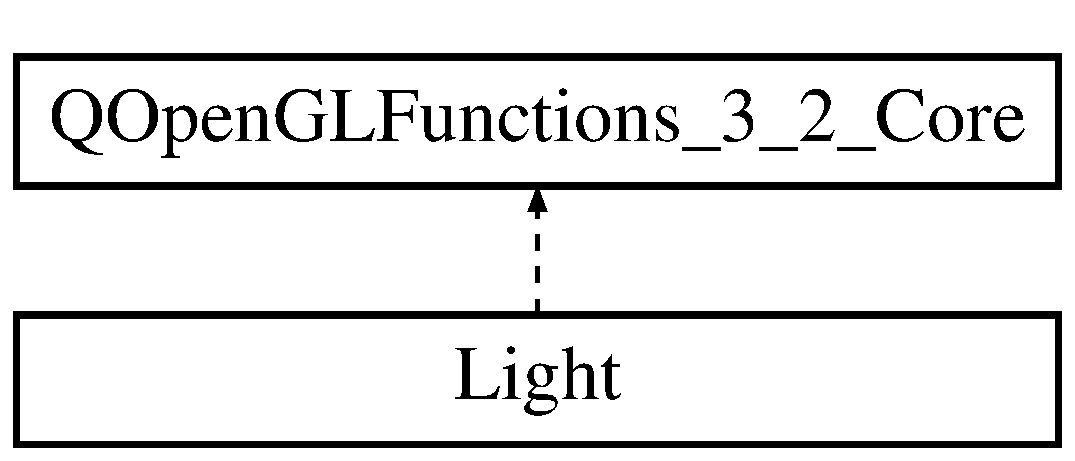
\includegraphics[height=2.000000cm]{class_light}
\end{center}
\end{figure}
\subsection*{Public Member Functions}
\begin{DoxyCompactItemize}
\item 
\hyperlink{class_light_aa7bcc37dee068f7266f86e07a3dfe4f0}{Light} (\hyperlink{structvec3}{vec3} position=\hyperlink{structvec3}{vec3}(0.\+0, 0.\+0, 0.\+0), \hyperlink{structvec3}{vec3} diffuse=\hyperlink{structvec3}{vec3}(0.\+8, 0.\+8, 0.\+8), \hyperlink{structvec3}{vec3} specular=\hyperlink{structvec3}{vec3}(0.\+8, 0.\+8, 0.\+8))
\begin{DoxyCompactList}\small\item\em Constructeur d'une lumière. \end{DoxyCompactList}\item 
\hyperlink{class_light_ad0e59fad13bb6cfadc25b2c477e9ddc7}{$\sim$\+Light} ()
\begin{DoxyCompactList}\small\item\em Destructeur. \end{DoxyCompactList}\item 
void \hyperlink{class_light_a9fcc4b3ffdeedbe214ee8384c7d311b9}{set} (G\+Lenum type, \hyperlink{structvec3}{vec3} value)
\begin{DoxyCompactList}\small\item\em Met à jour une composante de la lumière. \end{DoxyCompactList}\item 
\hyperlink{structvec3}{vec3} \hyperlink{class_light_ad0f5f939bc047e39c6deb2e264a5a2c1}{get} (G\+Lenum type) const 
\begin{DoxyCompactList}\small\item\em Récupère la valeur d'une composante de la lumière. \end{DoxyCompactList}\item 
\hyperlink{structvec3}{vec3} \& \hyperlink{class_light_a74a0381255c1c7e002ac583401a46de0}{get} (G\+Lenum type)
\begin{DoxyCompactList}\small\item\em Récupère la valeur d'une composante de la lumière. \end{DoxyCompactList}\item 
void \hyperlink{class_light_ade4c742c8ca2c014d74c659fa615ffd7}{update} (unsigned char number)
\begin{DoxyCompactList}\small\item\em Met à jour le shader avec les infos de la lumière. \end{DoxyCompactList}\end{DoxyCompactItemize}
\subsection*{Static Public Member Functions}
\begin{DoxyCompactItemize}
\item 
static void \hyperlink{class_light_a33a43afc95ed75a8970f523cb3f800fa}{disable} (unsigned char number)
\begin{DoxyCompactList}\small\item\em Désactive la lumière dans le shader. \end{DoxyCompactList}\item 
static void \hyperlink{class_light_a53ce58fd783207da18aa7dc3465841ac}{update\+Ambient} ()
\begin{DoxyCompactList}\small\item\em Met à jour la lumière ambient. \end{DoxyCompactList}\item 
static void \hyperlink{class_light_a1eae781d5e7a95c9dcc9bd76838496df}{ambient} (const \hyperlink{structvec3}{vec3} \&v)
\begin{DoxyCompactList}\small\item\em Modifie la composante ambient de la lumière. \end{DoxyCompactList}\item 
static \hyperlink{structvec3}{vec3} \& \hyperlink{class_light_a4f9a64ec04c9854d02a67cd2ceb6760c}{ambient} ()
\begin{DoxyCompactList}\small\item\em retourne le vecteur des composantes ambient \end{DoxyCompactList}\end{DoxyCompactItemize}
\subsection*{Private Attributes}
\begin{DoxyCompactItemize}
\item 
\hyperlink{structvec3}{vec3} \hyperlink{class_light_a3af8c823a869606782bd9e1872586b72}{\+\_\+position}
\item 
\hyperlink{structvec3}{vec3} \hyperlink{class_light_a32445f2054766ef532c29eb514b2599d}{\+\_\+diffuse}
\item 
\hyperlink{structvec3}{vec3} \hyperlink{class_light_a36414dc1e8a75b36652bc5a12b2ea43d}{\+\_\+specular}
\end{DoxyCompactItemize}
\subsection*{Static Private Attributes}
\begin{DoxyCompactItemize}
\item 
static \hyperlink{structvec3}{vec3} \hyperlink{class_light_ab139b739498b75944c99203027332ad9}{\+\_\+ambient}
\end{DoxyCompactItemize}


\subsection{Detailed Description}
Lumière pour la \hyperlink{class_scene}{Scene}. 

Gère une lumière pour la scène

\begin{DoxyWarning}{Warning}
seul les lumières positionnelles sont gérées pour l'instant 
\end{DoxyWarning}
\begin{DoxyRefDesc}{Todo}
\item[\hyperlink{todo__todo000001}{Todo}]attenuation de la lumière par lumière et plus globale \end{DoxyRefDesc}


\subsection{Constructor \& Destructor Documentation}
\hypertarget{class_light_aa7bcc37dee068f7266f86e07a3dfe4f0}{\index{Light@{Light}!Light@{Light}}
\index{Light@{Light}!Light@{Light}}
\subsubsection[{Light}]{\setlength{\rightskip}{0pt plus 5cm}Light\+::\+Light (
\begin{DoxyParamCaption}
\item[{{\bf vec3}}]{position = {\ttfamily {\bf vec3}(0.0,~0.0,~0.0)}, }
\item[{{\bf vec3}}]{diffuse = {\ttfamily {\bf vec3}(0.8,~0.8,~0.8)}, }
\item[{{\bf vec3}}]{specular = {\ttfamily {\bf vec3}(0.8,~0.8,~0.8)}}
\end{DoxyParamCaption}
)}}\label{class_light_aa7bcc37dee068f7266f86e07a3dfe4f0}


Constructeur d'une lumière. 


\begin{DoxyParams}{Parameters}
{\em position} & position de la lumière \\
\hline
{\em diffuse} & composante diffuse de la lumière \\
\hline
{\em specular} & composante spéculaire de la lumière \\
\hline
{\em number} & correspond au slot de la lumière qui sera utilisé dans le shader\\
\hline
\end{DoxyParams}
\begin{DoxyWarning}{Warning}
number doit appartenir à \mbox{[}0,7\mbox{]} 
\end{DoxyWarning}
\hypertarget{class_light_ad0e59fad13bb6cfadc25b2c477e9ddc7}{\index{Light@{Light}!````~Light@{$\sim$\+Light}}
\index{````~Light@{$\sim$\+Light}!Light@{Light}}
\subsubsection[{$\sim$\+Light}]{\setlength{\rightskip}{0pt plus 5cm}Light\+::$\sim$\+Light (
\begin{DoxyParamCaption}
{}
\end{DoxyParamCaption}
)}}\label{class_light_ad0e59fad13bb6cfadc25b2c477e9ddc7}


Destructeur. 

\begin{DoxyRefDesc}{Todo}
\item[\hyperlink{todo__todo000002}{Todo}]Vérifier que la lumière est désactivée dans tout les shader \end{DoxyRefDesc}


\subsection{Member Function Documentation}
\hypertarget{class_light_a1eae781d5e7a95c9dcc9bd76838496df}{\index{Light@{Light}!ambient@{ambient}}
\index{ambient@{ambient}!Light@{Light}}
\subsubsection[{ambient}]{\setlength{\rightskip}{0pt plus 5cm}static void Light\+::ambient (
\begin{DoxyParamCaption}
\item[{const {\bf vec3} \&}]{v}
\end{DoxyParamCaption}
)\hspace{0.3cm}{\ttfamily [inline]}, {\ttfamily [static]}}}\label{class_light_a1eae781d5e7a95c9dcc9bd76838496df}


Modifie la composante ambient de la lumière. 


\begin{DoxyParams}{Parameters}
{\em v} & nouvelle composante \\
\hline
\end{DoxyParams}
\hypertarget{class_light_a4f9a64ec04c9854d02a67cd2ceb6760c}{\index{Light@{Light}!ambient@{ambient}}
\index{ambient@{ambient}!Light@{Light}}
\subsubsection[{ambient}]{\setlength{\rightskip}{0pt plus 5cm}static {\bf vec3}\& Light\+::ambient (
\begin{DoxyParamCaption}
{}
\end{DoxyParamCaption}
)\hspace{0.3cm}{\ttfamily [inline]}, {\ttfamily [static]}}}\label{class_light_a4f9a64ec04c9854d02a67cd2ceb6760c}


retourne le vecteur des composantes ambient 

\hypertarget{class_light_a33a43afc95ed75a8970f523cb3f800fa}{\index{Light@{Light}!disable@{disable}}
\index{disable@{disable}!Light@{Light}}
\subsubsection[{disable}]{\setlength{\rightskip}{0pt plus 5cm}void Light\+::disable (
\begin{DoxyParamCaption}
\item[{unsigned char}]{number}
\end{DoxyParamCaption}
)\hspace{0.3cm}{\ttfamily [static]}}}\label{class_light_a33a43afc95ed75a8970f523cb3f800fa}


Désactive la lumière dans le shader. 


\begin{DoxyParams}{Parameters}
{\em number} & numéro de la lumière à désactiver \\
\hline
\end{DoxyParams}
\hypertarget{class_light_ad0f5f939bc047e39c6deb2e264a5a2c1}{\index{Light@{Light}!get@{get}}
\index{get@{get}!Light@{Light}}
\subsubsection[{get}]{\setlength{\rightskip}{0pt plus 5cm}{\bf vec3} Light\+::get (
\begin{DoxyParamCaption}
\item[{G\+Lenum}]{type}
\end{DoxyParamCaption}
) const}}\label{class_light_ad0f5f939bc047e39c6deb2e264a5a2c1}


Récupère la valeur d'une composante de la lumière. 


\begin{DoxyParams}{Parameters}
{\em type} & composante voulu, doit être parmis (G\+L\+\_\+\+P\+O\+S\+I\+T\+I\+O\+N, G\+L\+\_\+\+A\+M\+B\+I\+E\+N\+T, G\+L\+\_\+\+D\+I\+F\+F\+U\+S\+E, G\+L\+\_\+\+S\+P\+E\+C\+U\+L\+A\+R) \\
\hline
\end{DoxyParams}
\begin{DoxyReturn}{Returns}
valeur 
\end{DoxyReturn}
\hypertarget{class_light_a74a0381255c1c7e002ac583401a46de0}{\index{Light@{Light}!get@{get}}
\index{get@{get}!Light@{Light}}
\subsubsection[{get}]{\setlength{\rightskip}{0pt plus 5cm}{\bf vec3} \& Light\+::get (
\begin{DoxyParamCaption}
\item[{G\+Lenum}]{type}
\end{DoxyParamCaption}
)}}\label{class_light_a74a0381255c1c7e002ac583401a46de0}


Récupère la valeur d'une composante de la lumière. 


\begin{DoxyParams}{Parameters}
{\em type} & composante voulu, doit être parmis (G\+L\+\_\+\+P\+O\+S\+I\+T\+I\+O\+N, G\+L\+\_\+\+A\+M\+B\+I\+E\+N\+T, G\+L\+\_\+\+D\+I\+F\+F\+U\+S\+E, G\+L\+\_\+\+S\+P\+E\+C\+U\+L\+A\+R) \\
\hline
\end{DoxyParams}
\begin{DoxyReturn}{Returns}
valeur 
\end{DoxyReturn}
\begin{DoxyWarning}{Warning}
si le type n'est pas dans les 4 gérés résultat imprévisible 
\end{DoxyWarning}
\hypertarget{class_light_a9fcc4b3ffdeedbe214ee8384c7d311b9}{\index{Light@{Light}!set@{set}}
\index{set@{set}!Light@{Light}}
\subsubsection[{set}]{\setlength{\rightskip}{0pt plus 5cm}void Light\+::set (
\begin{DoxyParamCaption}
\item[{G\+Lenum}]{type, }
\item[{{\bf vec3}}]{value}
\end{DoxyParamCaption}
)}}\label{class_light_a9fcc4b3ffdeedbe214ee8384c7d311b9}


Met à jour une composante de la lumière. 


\begin{DoxyParams}{Parameters}
{\em type} & composante à modifier, doit être parmis (G\+L\+\_\+\+P\+O\+S\+I\+T\+I\+O\+N, G\+L\+\_\+\+A\+M\+B\+I\+E\+N\+T, G\+L\+\_\+\+D\+I\+F\+F\+U\+S\+E, G\+L\+\_\+\+S\+P\+E\+C\+U\+L\+A\+R) \\
\hline
{\em value} & valeur \\
\hline
\end{DoxyParams}
\hypertarget{class_light_ade4c742c8ca2c014d74c659fa615ffd7}{\index{Light@{Light}!update@{update}}
\index{update@{update}!Light@{Light}}
\subsubsection[{update}]{\setlength{\rightskip}{0pt plus 5cm}void Light\+::update (
\begin{DoxyParamCaption}
\item[{unsigned char}]{number}
\end{DoxyParamCaption}
)}}\label{class_light_ade4c742c8ca2c014d74c659fa615ffd7}


Met à jour le shader avec les infos de la lumière. 


\begin{DoxyParams}{Parameters}
{\em number} & slot de lumière à utiliser dans la shader \\
\hline
\end{DoxyParams}
\hypertarget{class_light_a53ce58fd783207da18aa7dc3465841ac}{\index{Light@{Light}!update\+Ambient@{update\+Ambient}}
\index{update\+Ambient@{update\+Ambient}!Light@{Light}}
\subsubsection[{update\+Ambient}]{\setlength{\rightskip}{0pt plus 5cm}void Light\+::update\+Ambient (
\begin{DoxyParamCaption}
{}
\end{DoxyParamCaption}
)\hspace{0.3cm}{\ttfamily [static]}}}\label{class_light_a53ce58fd783207da18aa7dc3465841ac}


Met à jour la lumière ambient. 



\subsection{Member Data Documentation}
\hypertarget{class_light_ab139b739498b75944c99203027332ad9}{\index{Light@{Light}!\+\_\+ambient@{\+\_\+ambient}}
\index{\+\_\+ambient@{\+\_\+ambient}!Light@{Light}}
\subsubsection[{\+\_\+ambient}]{\setlength{\rightskip}{0pt plus 5cm}{\bf vec3} Light\+::\+\_\+ambient\hspace{0.3cm}{\ttfamily [static]}, {\ttfamily [private]}}}\label{class_light_ab139b739498b75944c99203027332ad9}
La composante ambient est commune à toutes les lumières \hypertarget{class_light_a32445f2054766ef532c29eb514b2599d}{\index{Light@{Light}!\+\_\+diffuse@{\+\_\+diffuse}}
\index{\+\_\+diffuse@{\+\_\+diffuse}!Light@{Light}}
\subsubsection[{\+\_\+diffuse}]{\setlength{\rightskip}{0pt plus 5cm}{\bf vec3} Light\+::\+\_\+diffuse\hspace{0.3cm}{\ttfamily [private]}}}\label{class_light_a32445f2054766ef532c29eb514b2599d}
\hypertarget{class_light_a3af8c823a869606782bd9e1872586b72}{\index{Light@{Light}!\+\_\+position@{\+\_\+position}}
\index{\+\_\+position@{\+\_\+position}!Light@{Light}}
\subsubsection[{\+\_\+position}]{\setlength{\rightskip}{0pt plus 5cm}{\bf vec3} Light\+::\+\_\+position\hspace{0.3cm}{\ttfamily [private]}}}\label{class_light_a3af8c823a869606782bd9e1872586b72}
\hypertarget{class_light_a36414dc1e8a75b36652bc5a12b2ea43d}{\index{Light@{Light}!\+\_\+specular@{\+\_\+specular}}
\index{\+\_\+specular@{\+\_\+specular}!Light@{Light}}
\subsubsection[{\+\_\+specular}]{\setlength{\rightskip}{0pt plus 5cm}{\bf vec3} Light\+::\+\_\+specular\hspace{0.3cm}{\ttfamily [private]}}}\label{class_light_a36414dc1e8a75b36652bc5a12b2ea43d}


The documentation for this class was generated from the following files\+:\begin{DoxyCompactItemize}
\item 
scene/\hyperlink{light_8hpp}{light.\+hpp}\item 
scene/\hyperlink{light_8cpp}{light.\+cpp}\end{DoxyCompactItemize}

\hypertarget{structmat3}{\section{Référence de la structure mat3}
\label{structmat3}\index{mat3@{mat3}}
}


{\ttfamily \#include $<$helper.\+hpp$>$}



Graphe de collaboration de mat3\+:
\nopagebreak
\begin{figure}[H]
\begin{center}
\leavevmode
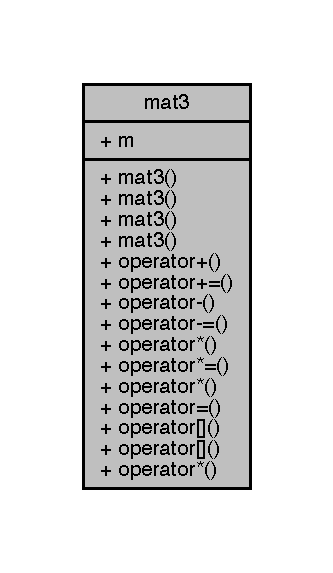
\includegraphics[width=160pt]{structmat3__coll__graph}
\end{center}
\end{figure}
\subsection*{Fonctions membres publiques}
\begin{DoxyCompactItemize}
\item 
\hyperlink{structmat3_a463027040addb1c56fe84c91b74b8d79}{mat3} ()
\item 
\hyperlink{structmat3_ae70cff0193ac1f77c61df7a2f4c00ef6}{mat3} (int)
\item 
\hyperlink{structmat3_ad5f393d1a6f7986207680e54e81f9906}{mat3} (float a, float b, float c, float d, float e, float f, float g, float h, float i)
\item 
\hyperlink{structmat3_aa761860db5b00723649f4751b34df952}{mat3} (const \hyperlink{structmat3}{mat3} \&)
\item 
\hyperlink{structmat3}{mat3} \hyperlink{structmat3_af00e96acb51cd53669a5d3a169d96e65}{operator+} (const \hyperlink{structmat3}{mat3} \&) const 
\item 
\hyperlink{structmat3}{mat3} \& \hyperlink{structmat3_a51c6ec6fd44fcd36022441064f6c285d}{operator+=} (const \hyperlink{structmat3}{mat3} \&)
\item 
\hyperlink{structmat3}{mat3} \hyperlink{structmat3_aa4a3e2abd71f23304e1069d3da0d60c0}{operator-\/} (const \hyperlink{structmat3}{mat3} \&) const 
\item 
\hyperlink{structmat3}{mat3} \& \hyperlink{structmat3_a1718976498fb7eddf36bbfebe76c0731}{operator-\/=} (const \hyperlink{structmat3}{mat3} \&)
\item 
\hyperlink{structmat3}{mat3} \hyperlink{structmat3_ab7b1c00fe3bfe66e48066f03a7c99cf5}{operator$\ast$} (const float) const 
\item 
\hyperlink{structmat3}{mat3} \& \hyperlink{structmat3_a782476876e4828df805c118734cef45f}{operator$\ast$=} (const float)
\item 
\hyperlink{structmat3}{mat3} \hyperlink{structmat3_affc4320ad21bf2276b32da8d96006a08}{operator$\ast$} (const \hyperlink{structmat3}{mat3} \&) const 
\item 
\hyperlink{structmat3}{mat3} \& \hyperlink{structmat3_aecf76e04b3d56cc333129fef2a832bb6}{operator=} (const \hyperlink{structmat3}{mat3} \&)
\item 
float \& \hyperlink{structmat3_afabeddfb3c711e2b0f806d9d8fa0534c}{operator\mbox{[}$\,$\mbox{]}} (int)
\item 
float \hyperlink{structmat3_ad61ce758d2b8def99daa43bded003023}{operator\mbox{[}$\,$\mbox{]}} (int) const 
\item 
\hyperlink{structvec3}{vec3} \hyperlink{structmat3_a08a5fd5fdb707a1ffe11b4e2c8b76beb}{operator$\ast$} (const \hyperlink{structvec3}{vec3} \&) const 
\end{DoxyCompactItemize}
\subsection*{Attributs publics}
\begin{DoxyCompactItemize}
\item 
float \hyperlink{structmat3_af5c67cec8668816c844bfd3f097f9eb2}{m} \mbox{[}9\mbox{]}
\end{DoxyCompactItemize}


\subsection{Documentation des constructeurs et destructeur}
\hypertarget{structmat3_a463027040addb1c56fe84c91b74b8d79}{\index{mat3@{mat3}!mat3@{mat3}}
\index{mat3@{mat3}!mat3@{mat3}}
\subsubsection[{mat3}]{\setlength{\rightskip}{0pt plus 5cm}mat3\+::mat3 (
\begin{DoxyParamCaption}
{}
\end{DoxyParamCaption}
)}}\label{structmat3_a463027040addb1c56fe84c91b74b8d79}


Voici le graphe des appelants de cette fonction \+:
\nopagebreak
\begin{figure}[H]
\begin{center}
\leavevmode
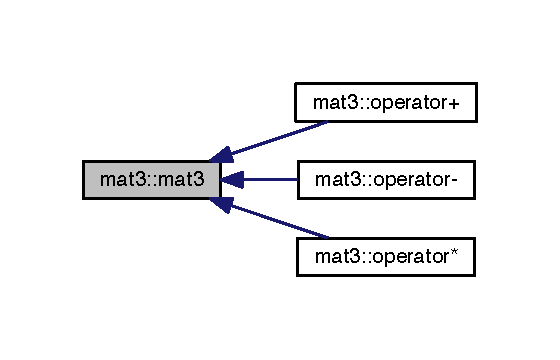
\includegraphics[width=269pt]{structmat3_a463027040addb1c56fe84c91b74b8d79_icgraph}
\end{center}
\end{figure}


\hypertarget{structmat3_ae70cff0193ac1f77c61df7a2f4c00ef6}{\index{mat3@{mat3}!mat3@{mat3}}
\index{mat3@{mat3}!mat3@{mat3}}
\subsubsection[{mat3}]{\setlength{\rightskip}{0pt plus 5cm}mat3\+::mat3 (
\begin{DoxyParamCaption}
\item[{int}]{}
\end{DoxyParamCaption}
)}}\label{structmat3_ae70cff0193ac1f77c61df7a2f4c00ef6}
\hypertarget{structmat3_ad5f393d1a6f7986207680e54e81f9906}{\index{mat3@{mat3}!mat3@{mat3}}
\index{mat3@{mat3}!mat3@{mat3}}
\subsubsection[{mat3}]{\setlength{\rightskip}{0pt plus 5cm}mat3\+::mat3 (
\begin{DoxyParamCaption}
\item[{float}]{a, }
\item[{float}]{b, }
\item[{float}]{c, }
\item[{float}]{d, }
\item[{float}]{e, }
\item[{float}]{f, }
\item[{float}]{g, }
\item[{float}]{h, }
\item[{float}]{i}
\end{DoxyParamCaption}
)}}\label{structmat3_ad5f393d1a6f7986207680e54e81f9906}
\hypertarget{structmat3_aa761860db5b00723649f4751b34df952}{\index{mat3@{mat3}!mat3@{mat3}}
\index{mat3@{mat3}!mat3@{mat3}}
\subsubsection[{mat3}]{\setlength{\rightskip}{0pt plus 5cm}mat3\+::mat3 (
\begin{DoxyParamCaption}
\item[{const {\bf mat3} \&}]{mm}
\end{DoxyParamCaption}
)}}\label{structmat3_aa761860db5b00723649f4751b34df952}


\subsection{Documentation des fonctions membres}
\hypertarget{structmat3_ab7b1c00fe3bfe66e48066f03a7c99cf5}{\index{mat3@{mat3}!operator$\ast$@{operator$\ast$}}
\index{operator$\ast$@{operator$\ast$}!mat3@{mat3}}
\subsubsection[{operator$\ast$}]{\setlength{\rightskip}{0pt plus 5cm}{\bf mat3} mat3\+::operator$\ast$ (
\begin{DoxyParamCaption}
\item[{const float}]{t}
\end{DoxyParamCaption}
) const}}\label{structmat3_ab7b1c00fe3bfe66e48066f03a7c99cf5}


Voici le graphe d'appel pour cette fonction \+:
\nopagebreak
\begin{figure}[H]
\begin{center}
\leavevmode
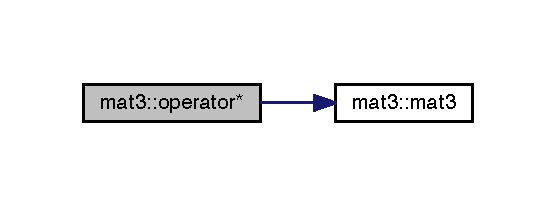
\includegraphics[width=267pt]{structmat3_ab7b1c00fe3bfe66e48066f03a7c99cf5_cgraph}
\end{center}
\end{figure}


\hypertarget{structmat3_affc4320ad21bf2276b32da8d96006a08}{\index{mat3@{mat3}!operator$\ast$@{operator$\ast$}}
\index{operator$\ast$@{operator$\ast$}!mat3@{mat3}}
\subsubsection[{operator$\ast$}]{\setlength{\rightskip}{0pt plus 5cm}{\bf mat3} mat3\+::operator$\ast$ (
\begin{DoxyParamCaption}
\item[{const {\bf mat3} \&}]{mm}
\end{DoxyParamCaption}
) const}}\label{structmat3_affc4320ad21bf2276b32da8d96006a08}


Voici le graphe d'appel pour cette fonction \+:
\nopagebreak
\begin{figure}[H]
\begin{center}
\leavevmode
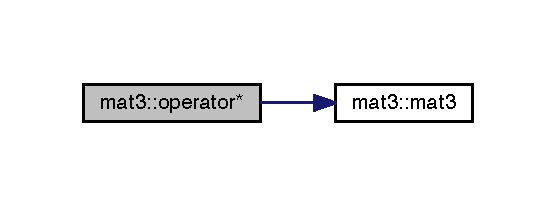
\includegraphics[width=267pt]{structmat3_affc4320ad21bf2276b32da8d96006a08_cgraph}
\end{center}
\end{figure}


\hypertarget{structmat3_a08a5fd5fdb707a1ffe11b4e2c8b76beb}{\index{mat3@{mat3}!operator$\ast$@{operator$\ast$}}
\index{operator$\ast$@{operator$\ast$}!mat3@{mat3}}
\subsubsection[{operator$\ast$}]{\setlength{\rightskip}{0pt plus 5cm}{\bf vec3} mat3\+::operator$\ast$ (
\begin{DoxyParamCaption}
\item[{const {\bf vec3} \&}]{vv}
\end{DoxyParamCaption}
) const}}\label{structmat3_a08a5fd5fdb707a1ffe11b4e2c8b76beb}
\hypertarget{structmat3_a782476876e4828df805c118734cef45f}{\index{mat3@{mat3}!operator$\ast$=@{operator$\ast$=}}
\index{operator$\ast$=@{operator$\ast$=}!mat3@{mat3}}
\subsubsection[{operator$\ast$=}]{\setlength{\rightskip}{0pt plus 5cm}{\bf mat3} \& mat3\+::operator$\ast$= (
\begin{DoxyParamCaption}
\item[{const float}]{t}
\end{DoxyParamCaption}
)}}\label{structmat3_a782476876e4828df805c118734cef45f}
\hypertarget{structmat3_af00e96acb51cd53669a5d3a169d96e65}{\index{mat3@{mat3}!operator+@{operator+}}
\index{operator+@{operator+}!mat3@{mat3}}
\subsubsection[{operator+}]{\setlength{\rightskip}{0pt plus 5cm}{\bf mat3} mat3\+::operator+ (
\begin{DoxyParamCaption}
\item[{const {\bf mat3} \&}]{mm}
\end{DoxyParamCaption}
) const}}\label{structmat3_af00e96acb51cd53669a5d3a169d96e65}


Voici le graphe d'appel pour cette fonction \+:
\nopagebreak
\begin{figure}[H]
\begin{center}
\leavevmode
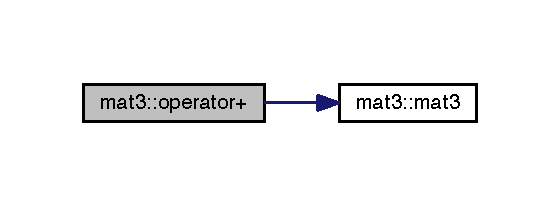
\includegraphics[width=269pt]{structmat3_af00e96acb51cd53669a5d3a169d96e65_cgraph}
\end{center}
\end{figure}


\hypertarget{structmat3_a51c6ec6fd44fcd36022441064f6c285d}{\index{mat3@{mat3}!operator+=@{operator+=}}
\index{operator+=@{operator+=}!mat3@{mat3}}
\subsubsection[{operator+=}]{\setlength{\rightskip}{0pt plus 5cm}{\bf mat3} \& mat3\+::operator+= (
\begin{DoxyParamCaption}
\item[{const {\bf mat3} \&}]{mm}
\end{DoxyParamCaption}
)}}\label{structmat3_a51c6ec6fd44fcd36022441064f6c285d}
\hypertarget{structmat3_aa4a3e2abd71f23304e1069d3da0d60c0}{\index{mat3@{mat3}!operator-\/@{operator-\/}}
\index{operator-\/@{operator-\/}!mat3@{mat3}}
\subsubsection[{operator-\/}]{\setlength{\rightskip}{0pt plus 5cm}{\bf mat3} mat3\+::operator-\/ (
\begin{DoxyParamCaption}
\item[{const {\bf mat3} \&}]{mm}
\end{DoxyParamCaption}
) const}}\label{structmat3_aa4a3e2abd71f23304e1069d3da0d60c0}


Voici le graphe d'appel pour cette fonction \+:
\nopagebreak
\begin{figure}[H]
\begin{center}
\leavevmode
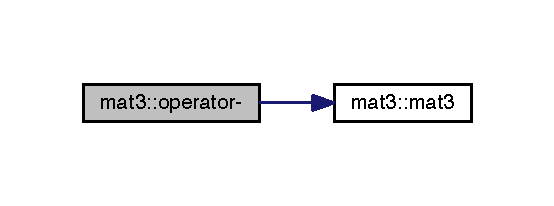
\includegraphics[width=266pt]{structmat3_aa4a3e2abd71f23304e1069d3da0d60c0_cgraph}
\end{center}
\end{figure}


\hypertarget{structmat3_a1718976498fb7eddf36bbfebe76c0731}{\index{mat3@{mat3}!operator-\/=@{operator-\/=}}
\index{operator-\/=@{operator-\/=}!mat3@{mat3}}
\subsubsection[{operator-\/=}]{\setlength{\rightskip}{0pt plus 5cm}{\bf mat3} \& mat3\+::operator-\/= (
\begin{DoxyParamCaption}
\item[{const {\bf mat3} \&}]{mm}
\end{DoxyParamCaption}
)}}\label{structmat3_a1718976498fb7eddf36bbfebe76c0731}
\hypertarget{structmat3_aecf76e04b3d56cc333129fef2a832bb6}{\index{mat3@{mat3}!operator=@{operator=}}
\index{operator=@{operator=}!mat3@{mat3}}
\subsubsection[{operator=}]{\setlength{\rightskip}{0pt plus 5cm}{\bf mat3} \& mat3\+::operator= (
\begin{DoxyParamCaption}
\item[{const {\bf mat3} \&}]{mm}
\end{DoxyParamCaption}
)}}\label{structmat3_aecf76e04b3d56cc333129fef2a832bb6}
\hypertarget{structmat3_afabeddfb3c711e2b0f806d9d8fa0534c}{\index{mat3@{mat3}!operator\mbox{[}$\,$\mbox{]}@{operator[]}}
\index{operator\mbox{[}$\,$\mbox{]}@{operator[]}!mat3@{mat3}}
\subsubsection[{operator[]}]{\setlength{\rightskip}{0pt plus 5cm}float \& mat3\+::operator\mbox{[}$\,$\mbox{]} (
\begin{DoxyParamCaption}
\item[{int}]{i}
\end{DoxyParamCaption}
)}}\label{structmat3_afabeddfb3c711e2b0f806d9d8fa0534c}
\hypertarget{structmat3_ad61ce758d2b8def99daa43bded003023}{\index{mat3@{mat3}!operator\mbox{[}$\,$\mbox{]}@{operator[]}}
\index{operator\mbox{[}$\,$\mbox{]}@{operator[]}!mat3@{mat3}}
\subsubsection[{operator[]}]{\setlength{\rightskip}{0pt plus 5cm}float mat3\+::operator\mbox{[}$\,$\mbox{]} (
\begin{DoxyParamCaption}
\item[{int}]{i}
\end{DoxyParamCaption}
) const}}\label{structmat3_ad61ce758d2b8def99daa43bded003023}


\subsection{Documentation des données membres}
\hypertarget{structmat3_af5c67cec8668816c844bfd3f097f9eb2}{\index{mat3@{mat3}!m@{m}}
\index{m@{m}!mat3@{mat3}}
\subsubsection[{m}]{\setlength{\rightskip}{0pt plus 5cm}float mat3\+::m\mbox{[}9\mbox{]}}}\label{structmat3_af5c67cec8668816c844bfd3f097f9eb2}


La documentation de cette structure a été générée à partir des fichiers suivants \+:\begin{DoxyCompactItemize}
\item 
\hyperlink{helper_8hpp}{helper.\+hpp}\item 
\hyperlink{helper_8cpp}{helper.\+cpp}\end{DoxyCompactItemize}

\hypertarget{structmat4}{\section{Référence de la structure mat4}
\label{structmat4}\index{mat4@{mat4}}
}


{\ttfamily \#include $<$helper.\+hpp$>$}



Graphe de collaboration de mat4\+:
\nopagebreak
\begin{figure}[H]
\begin{center}
\leavevmode
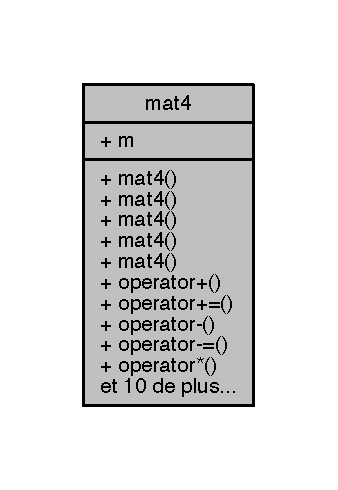
\includegraphics[width=162pt]{structmat4__coll__graph}
\end{center}
\end{figure}
\subsection*{Fonctions membres publiques}
\begin{DoxyCompactItemize}
\item 
\hyperlink{structmat4_acf3f0c37ff5c16e8fb1bfdde2bf87a0f}{mat4} ()
\item 
\hyperlink{structmat4_abbb345d8e90b7f5520a2854e4d171fad}{mat4} (int)
\item 
\hyperlink{structmat4_a9064945e550426ca0cbdc783abc159e3}{mat4} (float a, float b, float c, float d, float e, float f, float g, float h, float i, float j, float k, float l, float \hyperlink{structmat4_ab424bc8677a83f16bd30f4eaaecb6d3a}{m}, float n, float o, float p)
\item 
\hyperlink{structmat4_af9f2c48595cc3ef77b7264b6e1b80a9f}{mat4} (float $\ast$v)
\item 
\hyperlink{structmat4_a073e199b47525502781e3c36ef032dfb}{mat4} (const \hyperlink{structmat4}{mat4} \&)
\item 
\hyperlink{structmat4}{mat4} \hyperlink{structmat4_a1e09ab23f48d22eacf7480be5a6cea87}{operator+} (const \hyperlink{structmat4}{mat4} \&) const 
\item 
\hyperlink{structmat4}{mat4} \& \hyperlink{structmat4_a350e999ece6a2de198453342051887d5}{operator+=} (const \hyperlink{structmat4}{mat4} \&)
\item 
\hyperlink{structmat4}{mat4} \hyperlink{structmat4_a2ad7a60d812142642531b0ac06bf1c8e}{operator-\/} (const \hyperlink{structmat4}{mat4} \&) const 
\item 
\hyperlink{structmat4}{mat4} \& \hyperlink{structmat4_ac132dfe2e95f489dbd7164d91b535d7b}{operator-\/=} (const \hyperlink{structmat4}{mat4} \&)
\item 
\hyperlink{structmat4}{mat4} \hyperlink{structmat4_adfe86534dfda83be41334feaff6a9584}{operator$\ast$} (const float) const 
\item 
\hyperlink{structmat4}{mat4} \& \hyperlink{structmat4_ad0826521db3c90c1b3aba01c0e36d26e}{operator$\ast$=} (const float)
\item 
\hyperlink{structmat4}{mat4} \hyperlink{structmat4_a7cabd070852d9ccb840b20a6e4e492c2}{operator$\ast$} (const \hyperlink{structmat4}{mat4} \&) const 
\item 
\hyperlink{structmat4}{mat4} \& \hyperlink{structmat4_a480d75ddc6c5b4cd52f96eb9bde7966a}{operator$\ast$=} (const \hyperlink{structmat4}{mat4} \&)
\item 
\hyperlink{structmat4}{mat4} \& \hyperlink{structmat4_a22fc670708db72d05fc55bf02ad9bdcf}{operator=} (const \hyperlink{structmat4}{mat4} \&)
\item 
float \& \hyperlink{structmat4_ad4b21a373faeca027b94e0dce7f215ed}{operator\mbox{[}$\,$\mbox{]}} (int)
\item 
float \hyperlink{structmat4_a6fc70cc7bcabfc7127aef3a2a5cffaaa}{operator\mbox{[}$\,$\mbox{]}} (int) const 
\item 
\hyperlink{structvec4}{vec4} \hyperlink{structmat4_a74d5aa4c7f0bb9b4061551fbb06c120e}{operator$\ast$} (const \hyperlink{structvec4}{vec4} \&) const 
\item 
\hyperlink{structmat4}{mat4} \hyperlink{structmat4_aab816366c2233c95eac70b2eab11e8e2}{transpose} () const 
\item 
\hyperlink{structmat4}{mat4} \hyperlink{structmat4_a90efa7f6bcd321d1433629c8e6c09af3}{inverse} () const 
\item 
float \hyperlink{structmat4_a80b3a218af52e2cdcc5a216bfaa064b7}{det} () const 
\end{DoxyCompactItemize}
\subsection*{Attributs publics}
\begin{DoxyCompactItemize}
\item 
float \hyperlink{structmat4_ab424bc8677a83f16bd30f4eaaecb6d3a}{m} \mbox{[}16\mbox{]}
\end{DoxyCompactItemize}


\subsection{Documentation des constructeurs et destructeur}
\hypertarget{structmat4_acf3f0c37ff5c16e8fb1bfdde2bf87a0f}{\index{mat4@{mat4}!mat4@{mat4}}
\index{mat4@{mat4}!mat4@{mat4}}
\subsubsection[{mat4}]{\setlength{\rightskip}{0pt plus 5cm}mat4\+::mat4 (
\begin{DoxyParamCaption}
{}
\end{DoxyParamCaption}
)}}\label{structmat4_acf3f0c37ff5c16e8fb1bfdde2bf87a0f}


Voici le graphe des appelants de cette fonction \+:
\nopagebreak
\begin{figure}[H]
\begin{center}
\leavevmode
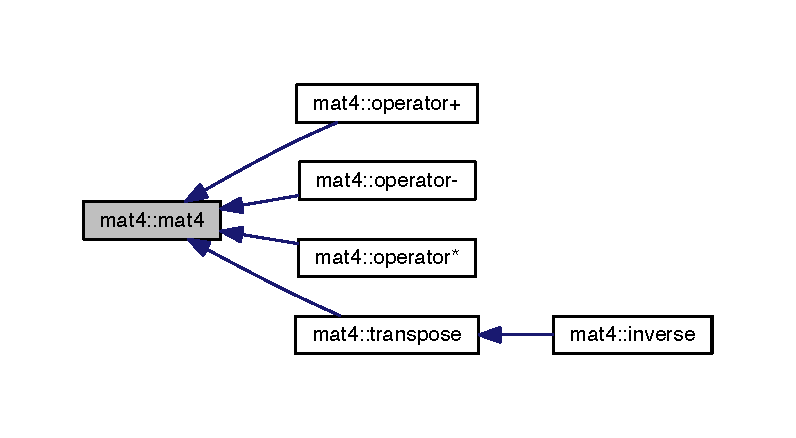
\includegraphics[width=350pt]{structmat4_acf3f0c37ff5c16e8fb1bfdde2bf87a0f_icgraph}
\end{center}
\end{figure}


\hypertarget{structmat4_abbb345d8e90b7f5520a2854e4d171fad}{\index{mat4@{mat4}!mat4@{mat4}}
\index{mat4@{mat4}!mat4@{mat4}}
\subsubsection[{mat4}]{\setlength{\rightskip}{0pt plus 5cm}mat4\+::mat4 (
\begin{DoxyParamCaption}
\item[{int}]{}
\end{DoxyParamCaption}
)}}\label{structmat4_abbb345d8e90b7f5520a2854e4d171fad}
\hypertarget{structmat4_a9064945e550426ca0cbdc783abc159e3}{\index{mat4@{mat4}!mat4@{mat4}}
\index{mat4@{mat4}!mat4@{mat4}}
\subsubsection[{mat4}]{\setlength{\rightskip}{0pt plus 5cm}mat4\+::mat4 (
\begin{DoxyParamCaption}
\item[{float}]{a, }
\item[{float}]{b, }
\item[{float}]{c, }
\item[{float}]{d, }
\item[{float}]{e, }
\item[{float}]{f, }
\item[{float}]{g, }
\item[{float}]{h, }
\item[{float}]{i, }
\item[{float}]{j, }
\item[{float}]{k, }
\item[{float}]{l, }
\item[{float}]{m, }
\item[{float}]{n, }
\item[{float}]{o, }
\item[{float}]{p}
\end{DoxyParamCaption}
)}}\label{structmat4_a9064945e550426ca0cbdc783abc159e3}
\hypertarget{structmat4_af9f2c48595cc3ef77b7264b6e1b80a9f}{\index{mat4@{mat4}!mat4@{mat4}}
\index{mat4@{mat4}!mat4@{mat4}}
\subsubsection[{mat4}]{\setlength{\rightskip}{0pt plus 5cm}mat4\+::mat4 (
\begin{DoxyParamCaption}
\item[{float $\ast$}]{v}
\end{DoxyParamCaption}
)}}\label{structmat4_af9f2c48595cc3ef77b7264b6e1b80a9f}
\hypertarget{structmat4_a073e199b47525502781e3c36ef032dfb}{\index{mat4@{mat4}!mat4@{mat4}}
\index{mat4@{mat4}!mat4@{mat4}}
\subsubsection[{mat4}]{\setlength{\rightskip}{0pt plus 5cm}mat4\+::mat4 (
\begin{DoxyParamCaption}
\item[{const {\bf mat4} \&}]{mm}
\end{DoxyParamCaption}
)}}\label{structmat4_a073e199b47525502781e3c36ef032dfb}


\subsection{Documentation des fonctions membres}
\hypertarget{structmat4_a80b3a218af52e2cdcc5a216bfaa064b7}{\index{mat4@{mat4}!det@{det}}
\index{det@{det}!mat4@{mat4}}
\subsubsection[{det}]{\setlength{\rightskip}{0pt plus 5cm}float mat4\+::det (
\begin{DoxyParamCaption}
{}
\end{DoxyParamCaption}
) const}}\label{structmat4_a80b3a218af52e2cdcc5a216bfaa064b7}


Voici le graphe des appelants de cette fonction \+:
\nopagebreak
\begin{figure}[H]
\begin{center}
\leavevmode
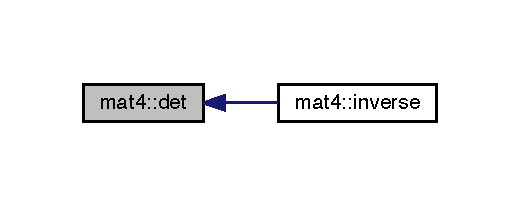
\includegraphics[width=250pt]{structmat4_a80b3a218af52e2cdcc5a216bfaa064b7_icgraph}
\end{center}
\end{figure}


\hypertarget{structmat4_a90efa7f6bcd321d1433629c8e6c09af3}{\index{mat4@{mat4}!inverse@{inverse}}
\index{inverse@{inverse}!mat4@{mat4}}
\subsubsection[{inverse}]{\setlength{\rightskip}{0pt plus 5cm}{\bf mat4} mat4\+::inverse (
\begin{DoxyParamCaption}
{}
\end{DoxyParamCaption}
) const}}\label{structmat4_a90efa7f6bcd321d1433629c8e6c09af3}


Voici le graphe d'appel pour cette fonction \+:
\nopagebreak
\begin{figure}[H]
\begin{center}
\leavevmode
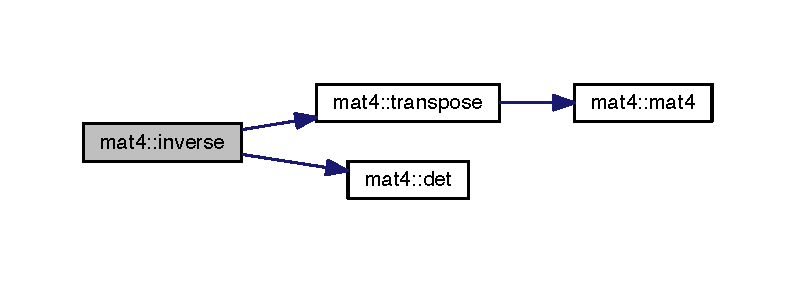
\includegraphics[width=350pt]{structmat4_a90efa7f6bcd321d1433629c8e6c09af3_cgraph}
\end{center}
\end{figure}


\hypertarget{structmat4_adfe86534dfda83be41334feaff6a9584}{\index{mat4@{mat4}!operator$\ast$@{operator$\ast$}}
\index{operator$\ast$@{operator$\ast$}!mat4@{mat4}}
\subsubsection[{operator$\ast$}]{\setlength{\rightskip}{0pt plus 5cm}{\bf mat4} mat4\+::operator$\ast$ (
\begin{DoxyParamCaption}
\item[{const float}]{t}
\end{DoxyParamCaption}
) const}}\label{structmat4_adfe86534dfda83be41334feaff6a9584}


Voici le graphe d'appel pour cette fonction \+:
\nopagebreak
\begin{figure}[H]
\begin{center}
\leavevmode
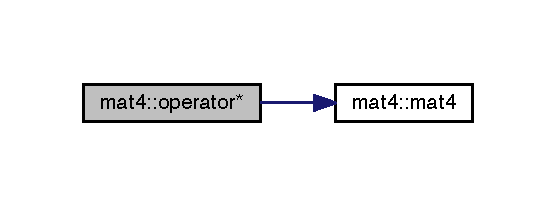
\includegraphics[width=267pt]{structmat4_adfe86534dfda83be41334feaff6a9584_cgraph}
\end{center}
\end{figure}


\hypertarget{structmat4_a7cabd070852d9ccb840b20a6e4e492c2}{\index{mat4@{mat4}!operator$\ast$@{operator$\ast$}}
\index{operator$\ast$@{operator$\ast$}!mat4@{mat4}}
\subsubsection[{operator$\ast$}]{\setlength{\rightskip}{0pt plus 5cm}{\bf mat4} mat4\+::operator$\ast$ (
\begin{DoxyParamCaption}
\item[{const {\bf mat4} \&}]{mm}
\end{DoxyParamCaption}
) const}}\label{structmat4_a7cabd070852d9ccb840b20a6e4e492c2}


Voici le graphe d'appel pour cette fonction \+:
\nopagebreak
\begin{figure}[H]
\begin{center}
\leavevmode
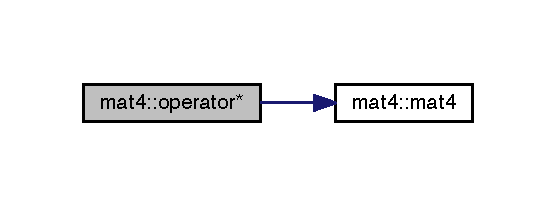
\includegraphics[width=267pt]{structmat4_a7cabd070852d9ccb840b20a6e4e492c2_cgraph}
\end{center}
\end{figure}


\hypertarget{structmat4_a74d5aa4c7f0bb9b4061551fbb06c120e}{\index{mat4@{mat4}!operator$\ast$@{operator$\ast$}}
\index{operator$\ast$@{operator$\ast$}!mat4@{mat4}}
\subsubsection[{operator$\ast$}]{\setlength{\rightskip}{0pt plus 5cm}{\bf vec4} mat4\+::operator$\ast$ (
\begin{DoxyParamCaption}
\item[{const {\bf vec4} \&}]{vv}
\end{DoxyParamCaption}
) const}}\label{structmat4_a74d5aa4c7f0bb9b4061551fbb06c120e}
\hypertarget{structmat4_ad0826521db3c90c1b3aba01c0e36d26e}{\index{mat4@{mat4}!operator$\ast$=@{operator$\ast$=}}
\index{operator$\ast$=@{operator$\ast$=}!mat4@{mat4}}
\subsubsection[{operator$\ast$=}]{\setlength{\rightskip}{0pt plus 5cm}{\bf mat4} \& mat4\+::operator$\ast$= (
\begin{DoxyParamCaption}
\item[{const float}]{t}
\end{DoxyParamCaption}
)}}\label{structmat4_ad0826521db3c90c1b3aba01c0e36d26e}
\hypertarget{structmat4_a480d75ddc6c5b4cd52f96eb9bde7966a}{\index{mat4@{mat4}!operator$\ast$=@{operator$\ast$=}}
\index{operator$\ast$=@{operator$\ast$=}!mat4@{mat4}}
\subsubsection[{operator$\ast$=}]{\setlength{\rightskip}{0pt plus 5cm}{\bf mat4} \& mat4\+::operator$\ast$= (
\begin{DoxyParamCaption}
\item[{const {\bf mat4} \&}]{mm}
\end{DoxyParamCaption}
)}}\label{structmat4_a480d75ddc6c5b4cd52f96eb9bde7966a}
\hypertarget{structmat4_a1e09ab23f48d22eacf7480be5a6cea87}{\index{mat4@{mat4}!operator+@{operator+}}
\index{operator+@{operator+}!mat4@{mat4}}
\subsubsection[{operator+}]{\setlength{\rightskip}{0pt plus 5cm}{\bf mat4} mat4\+::operator+ (
\begin{DoxyParamCaption}
\item[{const {\bf mat4} \&}]{mm}
\end{DoxyParamCaption}
) const}}\label{structmat4_a1e09ab23f48d22eacf7480be5a6cea87}


Voici le graphe d'appel pour cette fonction \+:
\nopagebreak
\begin{figure}[H]
\begin{center}
\leavevmode
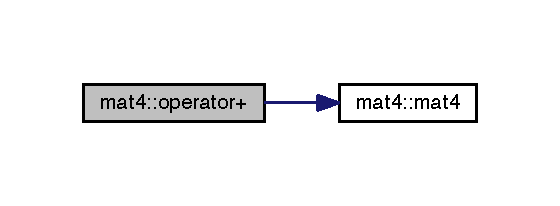
\includegraphics[width=269pt]{structmat4_a1e09ab23f48d22eacf7480be5a6cea87_cgraph}
\end{center}
\end{figure}


\hypertarget{structmat4_a350e999ece6a2de198453342051887d5}{\index{mat4@{mat4}!operator+=@{operator+=}}
\index{operator+=@{operator+=}!mat4@{mat4}}
\subsubsection[{operator+=}]{\setlength{\rightskip}{0pt plus 5cm}{\bf mat4} \& mat4\+::operator+= (
\begin{DoxyParamCaption}
\item[{const {\bf mat4} \&}]{mm}
\end{DoxyParamCaption}
)}}\label{structmat4_a350e999ece6a2de198453342051887d5}
\hypertarget{structmat4_a2ad7a60d812142642531b0ac06bf1c8e}{\index{mat4@{mat4}!operator-\/@{operator-\/}}
\index{operator-\/@{operator-\/}!mat4@{mat4}}
\subsubsection[{operator-\/}]{\setlength{\rightskip}{0pt plus 5cm}{\bf mat4} mat4\+::operator-\/ (
\begin{DoxyParamCaption}
\item[{const {\bf mat4} \&}]{mm}
\end{DoxyParamCaption}
) const}}\label{structmat4_a2ad7a60d812142642531b0ac06bf1c8e}


Voici le graphe d'appel pour cette fonction \+:
\nopagebreak
\begin{figure}[H]
\begin{center}
\leavevmode
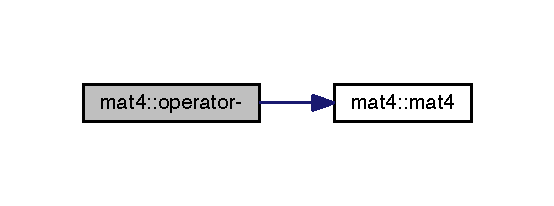
\includegraphics[width=266pt]{structmat4_a2ad7a60d812142642531b0ac06bf1c8e_cgraph}
\end{center}
\end{figure}


\hypertarget{structmat4_ac132dfe2e95f489dbd7164d91b535d7b}{\index{mat4@{mat4}!operator-\/=@{operator-\/=}}
\index{operator-\/=@{operator-\/=}!mat4@{mat4}}
\subsubsection[{operator-\/=}]{\setlength{\rightskip}{0pt plus 5cm}{\bf mat4} \& mat4\+::operator-\/= (
\begin{DoxyParamCaption}
\item[{const {\bf mat4} \&}]{mm}
\end{DoxyParamCaption}
)}}\label{structmat4_ac132dfe2e95f489dbd7164d91b535d7b}
\hypertarget{structmat4_a22fc670708db72d05fc55bf02ad9bdcf}{\index{mat4@{mat4}!operator=@{operator=}}
\index{operator=@{operator=}!mat4@{mat4}}
\subsubsection[{operator=}]{\setlength{\rightskip}{0pt plus 5cm}{\bf mat4} \& mat4\+::operator= (
\begin{DoxyParamCaption}
\item[{const {\bf mat4} \&}]{mm}
\end{DoxyParamCaption}
)}}\label{structmat4_a22fc670708db72d05fc55bf02ad9bdcf}
\hypertarget{structmat4_ad4b21a373faeca027b94e0dce7f215ed}{\index{mat4@{mat4}!operator\mbox{[}$\,$\mbox{]}@{operator[]}}
\index{operator\mbox{[}$\,$\mbox{]}@{operator[]}!mat4@{mat4}}
\subsubsection[{operator[]}]{\setlength{\rightskip}{0pt plus 5cm}float \& mat4\+::operator\mbox{[}$\,$\mbox{]} (
\begin{DoxyParamCaption}
\item[{int}]{i}
\end{DoxyParamCaption}
)}}\label{structmat4_ad4b21a373faeca027b94e0dce7f215ed}
\hypertarget{structmat4_a6fc70cc7bcabfc7127aef3a2a5cffaaa}{\index{mat4@{mat4}!operator\mbox{[}$\,$\mbox{]}@{operator[]}}
\index{operator\mbox{[}$\,$\mbox{]}@{operator[]}!mat4@{mat4}}
\subsubsection[{operator[]}]{\setlength{\rightskip}{0pt plus 5cm}float mat4\+::operator\mbox{[}$\,$\mbox{]} (
\begin{DoxyParamCaption}
\item[{int}]{i}
\end{DoxyParamCaption}
) const}}\label{structmat4_a6fc70cc7bcabfc7127aef3a2a5cffaaa}
\hypertarget{structmat4_aab816366c2233c95eac70b2eab11e8e2}{\index{mat4@{mat4}!transpose@{transpose}}
\index{transpose@{transpose}!mat4@{mat4}}
\subsubsection[{transpose}]{\setlength{\rightskip}{0pt plus 5cm}{\bf mat4} mat4\+::transpose (
\begin{DoxyParamCaption}
{}
\end{DoxyParamCaption}
) const}}\label{structmat4_aab816366c2233c95eac70b2eab11e8e2}


Voici le graphe d'appel pour cette fonction \+:
\nopagebreak
\begin{figure}[H]
\begin{center}
\leavevmode
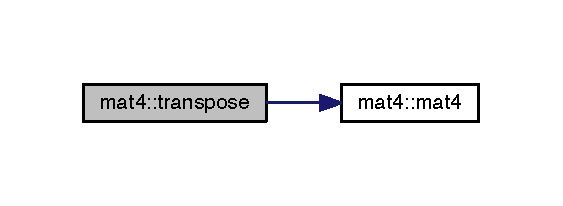
\includegraphics[width=270pt]{structmat4_aab816366c2233c95eac70b2eab11e8e2_cgraph}
\end{center}
\end{figure}




Voici le graphe des appelants de cette fonction \+:
\nopagebreak
\begin{figure}[H]
\begin{center}
\leavevmode
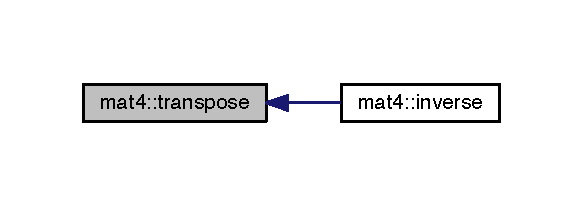
\includegraphics[width=280pt]{structmat4_aab816366c2233c95eac70b2eab11e8e2_icgraph}
\end{center}
\end{figure}




\subsection{Documentation des données membres}
\hypertarget{structmat4_ab424bc8677a83f16bd30f4eaaecb6d3a}{\index{mat4@{mat4}!m@{m}}
\index{m@{m}!mat4@{mat4}}
\subsubsection[{m}]{\setlength{\rightskip}{0pt plus 5cm}float mat4\+::m\mbox{[}16\mbox{]}}}\label{structmat4_ab424bc8677a83f16bd30f4eaaecb6d3a}


La documentation de cette structure a été générée à partir des fichiers suivants \+:\begin{DoxyCompactItemize}
\item 
\hyperlink{helper_8hpp}{helper.\+hpp}\item 
\hyperlink{helper_8cpp}{helper.\+cpp}\end{DoxyCompactItemize}

\hypertarget{class_material}{\section{Material Class Reference}
\label{class_material}\index{Material@{Material}}
}


Matériaux pour la \hyperlink{class_scene}{Scene}.  




{\ttfamily \#include $<$material.\+hpp$>$}

Inheritance diagram for Material\+:\begin{figure}[H]
\begin{center}
\leavevmode
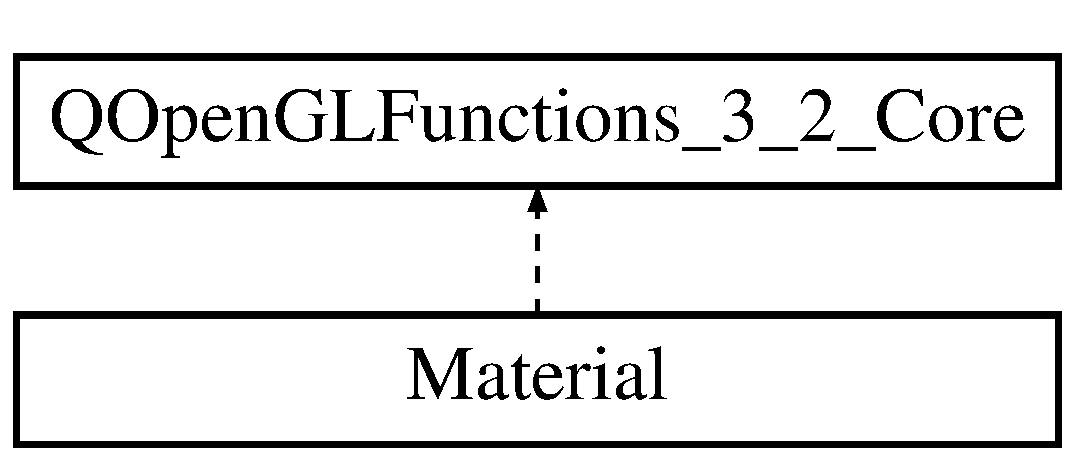
\includegraphics[height=2.000000cm]{class_material}
\end{center}
\end{figure}
\subsection*{Public Member Functions}
\begin{DoxyCompactItemize}
\item 
\hyperlink{class_material_a1692495b8e704a0ab17701365eb34b0f}{Material} (\hyperlink{structvec3}{vec3} ambient=\hyperlink{structvec3}{vec3}(0.\+2, 0.\+2, 0.\+2), \hyperlink{structvec3}{vec3} diffuse=\hyperlink{structvec3}{vec3}(0.\+8, 0.\+8, 0.\+8), \hyperlink{structvec3}{vec3} specular=\hyperlink{structvec3}{vec3}(0.\+8, 0.\+8, 0.\+8), float \hyperlink{class_material_a9a938aa96f0d5a5dc4d17d43cfd4b42b}{shininess}=0.\+0f, vec3 emissive=vec3(0.\+0, 0.\+0, 0.\+0))
\begin{DoxyCompactList}\small\item\em Constructeur. \end{DoxyCompactList}\item 
\hyperlink{class_material_a2c19452d71f54075df8f5405b03129f4}{$\sim$\+Material} ()
\begin{DoxyCompactList}\small\item\em Destructeur. \end{DoxyCompactList}\item 
void \hyperlink{class_material_a2ab92e03d9c90294cd28fff9b6a8cde0}{set} (G\+Lenum type, \hyperlink{structvec4}{vec4} value)
\begin{DoxyCompactList}\small\item\em Met à jour la composante du matériaux. \end{DoxyCompactList}\item 
void \hyperlink{class_material_a4f2227a6fb3f12c8618e399f93ab492c}{add\+Texture} (const Q\+String \&tex\+File, const Q\+String \&type)
\begin{DoxyCompactList}\small\item\em Charge une texture et l'associe à un slot. \end{DoxyCompactList}\item 
void \hyperlink{class_material_a3de47a95f13dc6f6306493516814762c}{set} (float \hyperlink{class_material_a9a938aa96f0d5a5dc4d17d43cfd4b42b}{shininess})
\begin{DoxyCompactList}\small\item\em Met à jour la shniness du \hyperlink{class_material}{Material}. \end{DoxyCompactList}\item 
\hyperlink{structvec3}{vec3} \hyperlink{class_material_a6b4b32cf23cbba3988becd840471a51c}{get} (G\+Lenum type) const 
\begin{DoxyCompactList}\small\item\em Récupère la valeur d'un champ. \end{DoxyCompactList}\item 
\hyperlink{structvec3}{vec3} \& \hyperlink{class_material_a229d118ec5602033bafbc1212a7b72ce}{get} (G\+Lenum type)
\begin{DoxyCompactList}\small\item\em Récupère la valeur d'un champ. \end{DoxyCompactList}\item 
float \hyperlink{class_material_a9a938aa96f0d5a5dc4d17d43cfd4b42b}{shininess} () const 
\begin{DoxyCompactList}\small\item\em Valeur du shininess. \end{DoxyCompactList}\item 
bool \hyperlink{class_material_a5a489f2fa09381b917c6bc3244e02877}{has\+Texture} (unsigned char type) const 
\item 
bool \hyperlink{class_material_aa07bc322b6904dd4ccf61620a0eb703c}{has\+Diffuse\+Texture} () const 
\item 
bool \hyperlink{class_material_ab1d0beef91e6149c0ebfc6c82b977889}{has\+Specular\+Texture} () const 
\item 
bool \hyperlink{class_material_a9bfe6c055d9af6f3ef029b62cc57e6a1}{has\+Normal\+Texture} () const 
\item 
Q\+String \hyperlink{class_material_a9305ced3fea7ab22cd25877e14cfb53c}{get\+Diffuse\+Texture\+Name} () const 
\begin{DoxyCompactList}\small\item\em Retourne le path de la texture diffuse. \end{DoxyCompactList}\item 
Q\+String \hyperlink{class_material_a0f33deb2e971506b9382d1ece4ff2fa6}{get\+Specular\+Texture\+Name} () const 
\begin{DoxyCompactList}\small\item\em Retourne le path de la texture spéculaire. \end{DoxyCompactList}\item 
Q\+String \hyperlink{class_material_ae72d423e9f07b3cc0388854e0ad2c1ca}{get\+Normal\+Texture\+Name} () const 
\begin{DoxyCompactList}\small\item\em Retourne le path de la normal map. \end{DoxyCompactList}\item 
void \hyperlink{class_material_a3f43fe7bcfa721fd8156adb151adf45c}{update} ()
\begin{DoxyCompactList}\small\item\em Met à jour le \hyperlink{class_material}{Material} courant dans le shader actif. \end{DoxyCompactList}\item 
bool \hyperlink{class_material_a3641da3931be722a809b13f882e2a703}{is\+From\+X\+M\+L} () const 
\begin{DoxyCompactList}\small\item\em Indique si le \hyperlink{class_material}{Material} a été chargé depuis le X\+M\+L ou pas. \end{DoxyCompactList}\item 
void \hyperlink{class_material_a806be90008bdccd18e0d657ac75ef61c}{from\+X\+M\+L} (bool b)
\begin{DoxyCompactList}\small\item\em Indique si le \hyperlink{class_material}{Material} est issu ou non du X\+M\+L. \end{DoxyCompactList}\end{DoxyCompactItemize}
\subsection*{Static Public Member Functions}
\begin{DoxyCompactItemize}
\item 
static void \hyperlink{class_material_ab350dd584b850dfc3e0c52201b5699e0}{clear} ()
\begin{DoxyCompactList}\small\item\em Libère les textures chargées. \end{DoxyCompactList}\end{DoxyCompactItemize}
\subsection*{Private Attributes}
\begin{DoxyCompactItemize}
\item 
\hyperlink{structvec3}{vec3} \hyperlink{class_material_a4c29044a3f7e8008eb3a0666c4ce09b9}{\+\_\+ambient}
\item 
\hyperlink{structvec3}{vec3} \hyperlink{class_material_a402005729d7d5a147d51dfcd691d2ffa}{\+\_\+diffuse}
\item 
\hyperlink{structvec3}{vec3} \hyperlink{class_material_af3e2839f5a712fba28111e00783af70f}{\+\_\+specular}
\item 
float \hyperlink{class_material_ae3f666b9de93b770232ebb5b1b3ee47e}{\+\_\+shininess}
\item 
\hyperlink{structvec3}{vec3} \hyperlink{class_material_a7c2eb5e499b3f46ec6e9d62f02653879}{\+\_\+emissive}
\item 
Q\+Open\+G\+L\+Texture $\ast$ \hyperlink{class_material_a522d07896a1363e987d09d8e4b66c156}{\+\_\+diffuse\+\_\+texture}
\item 
Q\+Open\+G\+L\+Texture $\ast$ \hyperlink{class_material_a15711d6d794b6ea122e38738fa73ba8a}{\+\_\+specular\+\_\+texture}
\item 
Q\+Open\+G\+L\+Texture $\ast$ \hyperlink{class_material_add78622071d92485dd37dbd1934453b3}{\+\_\+normal\+\_\+texture}
\item 
bool \hyperlink{class_material_a3a262cfbb40e19f79b29c61386e76f95}{\+\_\+from\+X\+M\+L}
\end{DoxyCompactItemize}
\subsection*{Static Private Attributes}
\begin{DoxyCompactItemize}
\item 
static Q\+Map$<$ Q\+String, \\*
Q\+Open\+G\+L\+Texture $\ast$ $>$ \hyperlink{class_material_a9f91b9fda835fed049df5c6959043623}{\+\_\+textures\+Loaded}
\end{DoxyCompactItemize}
\subsection*{Friends}
\begin{DoxyCompactItemize}
\item 
Q\+Debug \hyperlink{class_material_a6796ee577479f67459444fcd552e6c05}{operator$<$$<$} (Q\+Debug dbg, const \hyperlink{class_material}{Material} \&m)
\end{DoxyCompactItemize}


\subsection{Detailed Description}
Matériaux pour la \hyperlink{class_scene}{Scene}. 

Contient les informations nécessaire à la gestion d'un material pour la scène 

\subsection{Constructor \& Destructor Documentation}
\hypertarget{class_material_a1692495b8e704a0ab17701365eb34b0f}{\index{Material@{Material}!Material@{Material}}
\index{Material@{Material}!Material@{Material}}
\subsubsection[{Material}]{\setlength{\rightskip}{0pt plus 5cm}Material\+::\+Material (
\begin{DoxyParamCaption}
\item[{{\bf vec3}}]{ambient = {\ttfamily {\bf vec3}(0.2,~0.2,~0.2)}, }
\item[{{\bf vec3}}]{diffuse = {\ttfamily {\bf vec3}(0.8,~0.8,~0.8)}, }
\item[{{\bf vec3}}]{specular = {\ttfamily {\bf vec3}(0.8,~0.8,~0.8)}, }
\item[{float}]{shininess = {\ttfamily 0.0f}, }
\item[{{\bf vec3}}]{emissive = {\ttfamily {\bf vec3}(0.0,~0.0,~0.0)}}
\end{DoxyParamCaption}
)}}\label{class_material_a1692495b8e704a0ab17701365eb34b0f}


Constructeur. 

\begin{DoxyWarning}{Warning}
composante emissive pas encore gérée 
\end{DoxyWarning}
\hypertarget{class_material_a2c19452d71f54075df8f5405b03129f4}{\index{Material@{Material}!````~Material@{$\sim$\+Material}}
\index{````~Material@{$\sim$\+Material}!Material@{Material}}
\subsubsection[{$\sim$\+Material}]{\setlength{\rightskip}{0pt plus 5cm}Material\+::$\sim$\+Material (
\begin{DoxyParamCaption}
{}
\end{DoxyParamCaption}
)}}\label{class_material_a2c19452d71f54075df8f5405b03129f4}


Destructeur. 

\begin{DoxyRefDesc}{Todo}
\item[\hyperlink{todo__todo000003}{Todo}]Gérer libération de la texture quand plus utilisée \end{DoxyRefDesc}


\subsection{Member Function Documentation}
\hypertarget{class_material_a4f2227a6fb3f12c8618e399f93ab492c}{\index{Material@{Material}!add\+Texture@{add\+Texture}}
\index{add\+Texture@{add\+Texture}!Material@{Material}}
\subsubsection[{add\+Texture}]{\setlength{\rightskip}{0pt plus 5cm}void Material\+::add\+Texture (
\begin{DoxyParamCaption}
\item[{const Q\+String \&}]{tex\+File, }
\item[{const Q\+String \&}]{type}
\end{DoxyParamCaption}
)}}\label{class_material_a4f2227a6fb3f12c8618e399f93ab492c}


Charge une texture et l'associe à un slot. 

Charge une texture et l'associe à un slot pour le passage au shader


\begin{DoxyParams}{Parameters}
{\em tex\+File} & fichier de texture à charger \\
\hline
{\em int} & indice que la texture doit occuper \\
\hline
\end{DoxyParams}
\begin{DoxyWarning}{Warning}
Ecrase la texture à l'indice choisie 
\end{DoxyWarning}
\hypertarget{class_material_ab350dd584b850dfc3e0c52201b5699e0}{\index{Material@{Material}!clear@{clear}}
\index{clear@{clear}!Material@{Material}}
\subsubsection[{clear}]{\setlength{\rightskip}{0pt plus 5cm}void Material\+::clear (
\begin{DoxyParamCaption}
{}
\end{DoxyParamCaption}
)\hspace{0.3cm}{\ttfamily [static]}}}\label{class_material_ab350dd584b850dfc3e0c52201b5699e0}


Libère les textures chargées. 

\hypertarget{class_material_a806be90008bdccd18e0d657ac75ef61c}{\index{Material@{Material}!from\+X\+M\+L@{from\+X\+M\+L}}
\index{from\+X\+M\+L@{from\+X\+M\+L}!Material@{Material}}
\subsubsection[{from\+X\+M\+L}]{\setlength{\rightskip}{0pt plus 5cm}void Material\+::from\+X\+M\+L (
\begin{DoxyParamCaption}
\item[{bool}]{b}
\end{DoxyParamCaption}
)\hspace{0.3cm}{\ttfamily [inline]}}}\label{class_material_a806be90008bdccd18e0d657ac75ef61c}


Indique si le \hyperlink{class_material}{Material} est issu ou non du X\+M\+L. 

\hypertarget{class_material_a6b4b32cf23cbba3988becd840471a51c}{\index{Material@{Material}!get@{get}}
\index{get@{get}!Material@{Material}}
\subsubsection[{get}]{\setlength{\rightskip}{0pt plus 5cm}{\bf vec3} Material\+::get (
\begin{DoxyParamCaption}
\item[{G\+Lenum}]{type}
\end{DoxyParamCaption}
) const}}\label{class_material_a6b4b32cf23cbba3988becd840471a51c}


Récupère la valeur d'un champ. 


\begin{DoxyParams}{Parameters}
{\em type} & doit être parmis G\+L\+\_\+\+A\+M\+B\+I\+E\+N\+T, G\+L\+\_\+\+D\+I\+F\+F\+U\+S\+E, G\+L\+\_\+\+S\+P\+E\+C\+U\+L\+A\+R \\
\hline
\end{DoxyParams}
\begin{DoxyReturn}{Returns}
dans le cas de G\+L\+\_\+\+A\+M\+B\+I\+E\+N\+T, G\+L\+\_\+\+D\+I\+F\+F\+U\+S\+E, G\+L\+\_\+\+S\+P\+E\+C\+U\+L\+A\+R retourne un \hyperlink{structvec3}{vec3} correspondant à la composante, retourne \hyperlink{helper_8hpp_a8d45e9fbe94ddf3c3291116b8fce15c5}{vec4()} autrement 
\end{DoxyReturn}
\hypertarget{class_material_a229d118ec5602033bafbc1212a7b72ce}{\index{Material@{Material}!get@{get}}
\index{get@{get}!Material@{Material}}
\subsubsection[{get}]{\setlength{\rightskip}{0pt plus 5cm}{\bf vec3} \& Material\+::get (
\begin{DoxyParamCaption}
\item[{G\+Lenum}]{type}
\end{DoxyParamCaption}
)}}\label{class_material_a229d118ec5602033bafbc1212a7b72ce}


Récupère la valeur d'un champ. 


\begin{DoxyParams}{Parameters}
{\em type} & doit être parmis G\+L\+\_\+\+A\+M\+B\+I\+E\+N\+T, G\+L\+\_\+\+D\+I\+F\+F\+U\+S\+E, G\+L\+\_\+\+S\+P\+E\+C\+U\+L\+A\+R \\
\hline
\end{DoxyParams}
\begin{DoxyReturn}{Returns}
dans le cas de G\+L\+\_\+\+A\+M\+B\+I\+E\+N\+T, G\+L\+\_\+\+D\+I\+F\+F\+U\+S\+E, G\+L\+\_\+\+S\+P\+E\+C\+U\+L\+A\+R retourne un \hyperlink{structvec3}{vec3} correspondant à la composante, retourne \hyperlink{helper_8hpp_a8d45e9fbe94ddf3c3291116b8fce15c5}{vec4()} autrement 
\end{DoxyReturn}
\hypertarget{class_material_a9305ced3fea7ab22cd25877e14cfb53c}{\index{Material@{Material}!get\+Diffuse\+Texture\+Name@{get\+Diffuse\+Texture\+Name}}
\index{get\+Diffuse\+Texture\+Name@{get\+Diffuse\+Texture\+Name}!Material@{Material}}
\subsubsection[{get\+Diffuse\+Texture\+Name}]{\setlength{\rightskip}{0pt plus 5cm}Q\+String Material\+::get\+Diffuse\+Texture\+Name (
\begin{DoxyParamCaption}
{}
\end{DoxyParamCaption}
) const}}\label{class_material_a9305ced3fea7ab22cd25877e14cfb53c}


Retourne le path de la texture diffuse. 

\begin{DoxyReturn}{Returns}
nom de la texture diffuse 
\end{DoxyReturn}
\hypertarget{class_material_ae72d423e9f07b3cc0388854e0ad2c1ca}{\index{Material@{Material}!get\+Normal\+Texture\+Name@{get\+Normal\+Texture\+Name}}
\index{get\+Normal\+Texture\+Name@{get\+Normal\+Texture\+Name}!Material@{Material}}
\subsubsection[{get\+Normal\+Texture\+Name}]{\setlength{\rightskip}{0pt plus 5cm}Q\+String Material\+::get\+Normal\+Texture\+Name (
\begin{DoxyParamCaption}
{}
\end{DoxyParamCaption}
) const}}\label{class_material_ae72d423e9f07b3cc0388854e0ad2c1ca}


Retourne le path de la normal map. 

\begin{DoxyReturn}{Returns}
nom de la normal map 
\end{DoxyReturn}
\hypertarget{class_material_a0f33deb2e971506b9382d1ece4ff2fa6}{\index{Material@{Material}!get\+Specular\+Texture\+Name@{get\+Specular\+Texture\+Name}}
\index{get\+Specular\+Texture\+Name@{get\+Specular\+Texture\+Name}!Material@{Material}}
\subsubsection[{get\+Specular\+Texture\+Name}]{\setlength{\rightskip}{0pt plus 5cm}Q\+String Material\+::get\+Specular\+Texture\+Name (
\begin{DoxyParamCaption}
{}
\end{DoxyParamCaption}
) const}}\label{class_material_a0f33deb2e971506b9382d1ece4ff2fa6}


Retourne le path de la texture spéculaire. 

\begin{DoxyReturn}{Returns}
nom de la texture spéculaire 
\end{DoxyReturn}
\hypertarget{class_material_aa07bc322b6904dd4ccf61620a0eb703c}{\index{Material@{Material}!has\+Diffuse\+Texture@{has\+Diffuse\+Texture}}
\index{has\+Diffuse\+Texture@{has\+Diffuse\+Texture}!Material@{Material}}
\subsubsection[{has\+Diffuse\+Texture}]{\setlength{\rightskip}{0pt plus 5cm}bool Material\+::has\+Diffuse\+Texture (
\begin{DoxyParamCaption}
{}
\end{DoxyParamCaption}
) const}}\label{class_material_aa07bc322b6904dd4ccf61620a0eb703c}
\hypertarget{class_material_a9bfe6c055d9af6f3ef029b62cc57e6a1}{\index{Material@{Material}!has\+Normal\+Texture@{has\+Normal\+Texture}}
\index{has\+Normal\+Texture@{has\+Normal\+Texture}!Material@{Material}}
\subsubsection[{has\+Normal\+Texture}]{\setlength{\rightskip}{0pt plus 5cm}bool Material\+::has\+Normal\+Texture (
\begin{DoxyParamCaption}
{}
\end{DoxyParamCaption}
) const}}\label{class_material_a9bfe6c055d9af6f3ef029b62cc57e6a1}
\hypertarget{class_material_ab1d0beef91e6149c0ebfc6c82b977889}{\index{Material@{Material}!has\+Specular\+Texture@{has\+Specular\+Texture}}
\index{has\+Specular\+Texture@{has\+Specular\+Texture}!Material@{Material}}
\subsubsection[{has\+Specular\+Texture}]{\setlength{\rightskip}{0pt plus 5cm}bool Material\+::has\+Specular\+Texture (
\begin{DoxyParamCaption}
{}
\end{DoxyParamCaption}
) const}}\label{class_material_ab1d0beef91e6149c0ebfc6c82b977889}
\hypertarget{class_material_a5a489f2fa09381b917c6bc3244e02877}{\index{Material@{Material}!has\+Texture@{has\+Texture}}
\index{has\+Texture@{has\+Texture}!Material@{Material}}
\subsubsection[{has\+Texture}]{\setlength{\rightskip}{0pt plus 5cm}bool Material\+::has\+Texture (
\begin{DoxyParamCaption}
\item[{unsigned char}]{type}
\end{DoxyParamCaption}
) const}}\label{class_material_a5a489f2fa09381b917c6bc3244e02877}
\hypertarget{class_material_a3641da3931be722a809b13f882e2a703}{\index{Material@{Material}!is\+From\+X\+M\+L@{is\+From\+X\+M\+L}}
\index{is\+From\+X\+M\+L@{is\+From\+X\+M\+L}!Material@{Material}}
\subsubsection[{is\+From\+X\+M\+L}]{\setlength{\rightskip}{0pt plus 5cm}bool Material\+::is\+From\+X\+M\+L (
\begin{DoxyParamCaption}
{}
\end{DoxyParamCaption}
) const\hspace{0.3cm}{\ttfamily [inline]}}}\label{class_material_a3641da3931be722a809b13f882e2a703}


Indique si le \hyperlink{class_material}{Material} a été chargé depuis le X\+M\+L ou pas. 

\hypertarget{class_material_a2ab92e03d9c90294cd28fff9b6a8cde0}{\index{Material@{Material}!set@{set}}
\index{set@{set}!Material@{Material}}
\subsubsection[{set}]{\setlength{\rightskip}{0pt plus 5cm}void Material\+::set (
\begin{DoxyParamCaption}
\item[{G\+Lenum}]{type, }
\item[{{\bf vec4}}]{value}
\end{DoxyParamCaption}
)}}\label{class_material_a2ab92e03d9c90294cd28fff9b6a8cde0}


Met à jour la composante du matériaux. 


\begin{DoxyParams}{Parameters}
{\em type} & la composante qui sera mise à jour, doit être parmis G\+L\+\_\+\+A\+M\+B\+I\+E\+N\+T, G\+L\+\_\+\+D\+I\+F\+F\+U\+S\+E, G\+L\+\_\+\+S\+P\+E\+C\+U\+L\+A\+R, G\+L\+\_\+\+E\+M\+I\+S\+S\+I\+O\+N \\
\hline
{\em value} & valeur \\
\hline
\end{DoxyParams}
\hypertarget{class_material_a3de47a95f13dc6f6306493516814762c}{\index{Material@{Material}!set@{set}}
\index{set@{set}!Material@{Material}}
\subsubsection[{set}]{\setlength{\rightskip}{0pt plus 5cm}void Material\+::set (
\begin{DoxyParamCaption}
\item[{float}]{shininess}
\end{DoxyParamCaption}
)}}\label{class_material_a3de47a95f13dc6f6306493516814762c}


Met à jour la shniness du \hyperlink{class_material}{Material}. 


\begin{DoxyParams}{Parameters}
{\em shininess} & valeur \\
\hline
\end{DoxyParams}
\hypertarget{class_material_a9a938aa96f0d5a5dc4d17d43cfd4b42b}{\index{Material@{Material}!shininess@{shininess}}
\index{shininess@{shininess}!Material@{Material}}
\subsubsection[{shininess}]{\setlength{\rightskip}{0pt plus 5cm}float Material\+::shininess (
\begin{DoxyParamCaption}
{}
\end{DoxyParamCaption}
) const}}\label{class_material_a9a938aa96f0d5a5dc4d17d43cfd4b42b}


Valeur du shininess. 

\begin{DoxyReturn}{Returns}
valeur du G\+L\+\_\+\+S\+H\+I\+N\+I\+N\+E\+S\+S 
\end{DoxyReturn}
\hypertarget{class_material_a3f43fe7bcfa721fd8156adb151adf45c}{\index{Material@{Material}!update@{update}}
\index{update@{update}!Material@{Material}}
\subsubsection[{update}]{\setlength{\rightskip}{0pt plus 5cm}void Material\+::update (
\begin{DoxyParamCaption}
{}
\end{DoxyParamCaption}
)}}\label{class_material_a3f43fe7bcfa721fd8156adb151adf45c}


Met à jour le \hyperlink{class_material}{Material} courant dans le shader actif. 



\subsection{Friends And Related Function Documentation}
\hypertarget{class_material_a6796ee577479f67459444fcd552e6c05}{\index{Material@{Material}!operator$<$$<$@{operator$<$$<$}}
\index{operator$<$$<$@{operator$<$$<$}!Material@{Material}}
\subsubsection[{operator$<$$<$}]{\setlength{\rightskip}{0pt plus 5cm}Q\+Debug operator$<$$<$ (
\begin{DoxyParamCaption}
\item[{Q\+Debug}]{dbg, }
\item[{const {\bf Material} \&}]{m}
\end{DoxyParamCaption}
)\hspace{0.3cm}{\ttfamily [friend]}}}\label{class_material_a6796ee577479f67459444fcd552e6c05}


\subsection{Member Data Documentation}
\hypertarget{class_material_a4c29044a3f7e8008eb3a0666c4ce09b9}{\index{Material@{Material}!\+\_\+ambient@{\+\_\+ambient}}
\index{\+\_\+ambient@{\+\_\+ambient}!Material@{Material}}
\subsubsection[{\+\_\+ambient}]{\setlength{\rightskip}{0pt plus 5cm}{\bf vec3} Material\+::\+\_\+ambient\hspace{0.3cm}{\ttfamily [private]}}}\label{class_material_a4c29044a3f7e8008eb3a0666c4ce09b9}
\hypertarget{class_material_a402005729d7d5a147d51dfcd691d2ffa}{\index{Material@{Material}!\+\_\+diffuse@{\+\_\+diffuse}}
\index{\+\_\+diffuse@{\+\_\+diffuse}!Material@{Material}}
\subsubsection[{\+\_\+diffuse}]{\setlength{\rightskip}{0pt plus 5cm}{\bf vec3} Material\+::\+\_\+diffuse\hspace{0.3cm}{\ttfamily [private]}}}\label{class_material_a402005729d7d5a147d51dfcd691d2ffa}
\hypertarget{class_material_a522d07896a1363e987d09d8e4b66c156}{\index{Material@{Material}!\+\_\+diffuse\+\_\+texture@{\+\_\+diffuse\+\_\+texture}}
\index{\+\_\+diffuse\+\_\+texture@{\+\_\+diffuse\+\_\+texture}!Material@{Material}}
\subsubsection[{\+\_\+diffuse\+\_\+texture}]{\setlength{\rightskip}{0pt plus 5cm}Q\+Open\+G\+L\+Texture$\ast$ Material\+::\+\_\+diffuse\+\_\+texture\hspace{0.3cm}{\ttfamily [private]}}}\label{class_material_a522d07896a1363e987d09d8e4b66c156}
\hypertarget{class_material_a7c2eb5e499b3f46ec6e9d62f02653879}{\index{Material@{Material}!\+\_\+emissive@{\+\_\+emissive}}
\index{\+\_\+emissive@{\+\_\+emissive}!Material@{Material}}
\subsubsection[{\+\_\+emissive}]{\setlength{\rightskip}{0pt plus 5cm}{\bf vec3} Material\+::\+\_\+emissive\hspace{0.3cm}{\ttfamily [private]}}}\label{class_material_a7c2eb5e499b3f46ec6e9d62f02653879}
\hypertarget{class_material_a3a262cfbb40e19f79b29c61386e76f95}{\index{Material@{Material}!\+\_\+from\+X\+M\+L@{\+\_\+from\+X\+M\+L}}
\index{\+\_\+from\+X\+M\+L@{\+\_\+from\+X\+M\+L}!Material@{Material}}
\subsubsection[{\+\_\+from\+X\+M\+L}]{\setlength{\rightskip}{0pt plus 5cm}bool Material\+::\+\_\+from\+X\+M\+L\hspace{0.3cm}{\ttfamily [private]}}}\label{class_material_a3a262cfbb40e19f79b29c61386e76f95}
\hypertarget{class_material_add78622071d92485dd37dbd1934453b3}{\index{Material@{Material}!\+\_\+normal\+\_\+texture@{\+\_\+normal\+\_\+texture}}
\index{\+\_\+normal\+\_\+texture@{\+\_\+normal\+\_\+texture}!Material@{Material}}
\subsubsection[{\+\_\+normal\+\_\+texture}]{\setlength{\rightskip}{0pt plus 5cm}Q\+Open\+G\+L\+Texture$\ast$ Material\+::\+\_\+normal\+\_\+texture\hspace{0.3cm}{\ttfamily [private]}}}\label{class_material_add78622071d92485dd37dbd1934453b3}
\hypertarget{class_material_ae3f666b9de93b770232ebb5b1b3ee47e}{\index{Material@{Material}!\+\_\+shininess@{\+\_\+shininess}}
\index{\+\_\+shininess@{\+\_\+shininess}!Material@{Material}}
\subsubsection[{\+\_\+shininess}]{\setlength{\rightskip}{0pt plus 5cm}float Material\+::\+\_\+shininess\hspace{0.3cm}{\ttfamily [private]}}}\label{class_material_ae3f666b9de93b770232ebb5b1b3ee47e}
\hypertarget{class_material_af3e2839f5a712fba28111e00783af70f}{\index{Material@{Material}!\+\_\+specular@{\+\_\+specular}}
\index{\+\_\+specular@{\+\_\+specular}!Material@{Material}}
\subsubsection[{\+\_\+specular}]{\setlength{\rightskip}{0pt plus 5cm}{\bf vec3} Material\+::\+\_\+specular\hspace{0.3cm}{\ttfamily [private]}}}\label{class_material_af3e2839f5a712fba28111e00783af70f}
\hypertarget{class_material_a15711d6d794b6ea122e38738fa73ba8a}{\index{Material@{Material}!\+\_\+specular\+\_\+texture@{\+\_\+specular\+\_\+texture}}
\index{\+\_\+specular\+\_\+texture@{\+\_\+specular\+\_\+texture}!Material@{Material}}
\subsubsection[{\+\_\+specular\+\_\+texture}]{\setlength{\rightskip}{0pt plus 5cm}Q\+Open\+G\+L\+Texture$\ast$ Material\+::\+\_\+specular\+\_\+texture\hspace{0.3cm}{\ttfamily [private]}}}\label{class_material_a15711d6d794b6ea122e38738fa73ba8a}
\hypertarget{class_material_a9f91b9fda835fed049df5c6959043623}{\index{Material@{Material}!\+\_\+textures\+Loaded@{\+\_\+textures\+Loaded}}
\index{\+\_\+textures\+Loaded@{\+\_\+textures\+Loaded}!Material@{Material}}
\subsubsection[{\+\_\+textures\+Loaded}]{\setlength{\rightskip}{0pt plus 5cm}Q\+Map$<$ Q\+String, Q\+Open\+G\+L\+Texture $\ast$ $>$ Material\+::\+\_\+textures\+Loaded\hspace{0.3cm}{\ttfamily [static]}, {\ttfamily [private]}}}\label{class_material_a9f91b9fda835fed049df5c6959043623}
Ensemble des textures déjà chargées pour réutilisation 

The documentation for this class was generated from the following files\+:\begin{DoxyCompactItemize}
\item 
scene/\hyperlink{material_8hpp}{material.\+hpp}\item 
scene/\hyperlink{material_8cpp}{material.\+cpp}\end{DoxyCompactItemize}

\hypertarget{class_mesh}{\section{Mesh Class Reference}
\label{class_mesh}\index{Mesh@{Mesh}}
}


Charge un modèle 3\+D.  




{\ttfamily \#include $<$mesh.\+hpp$>$}

Inheritance diagram for Mesh\+:\begin{figure}[H]
\begin{center}
\leavevmode
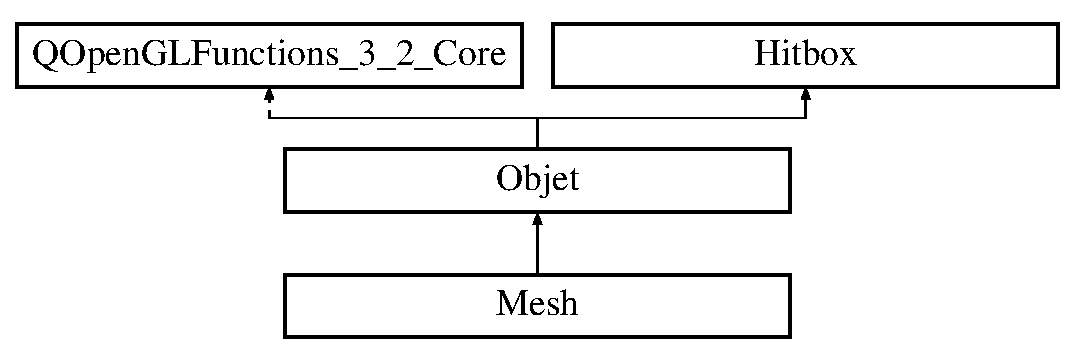
\includegraphics[height=3.000000cm]{class_mesh}
\end{center}
\end{figure}
\subsection*{Classes}
\begin{DoxyCompactItemize}
\item 
struct \hyperlink{struct_mesh_1_1_mesh_info}{Mesh\+Info}
\end{DoxyCompactItemize}
\subsection*{Public Member Functions}
\begin{DoxyCompactItemize}
\item 
\hyperlink{class_mesh_a5efe4da1a4c0971cfb037bd70304c303}{$\sim$\+Mesh} ()
\begin{DoxyCompactList}\small\item\em Destructeur. \end{DoxyCompactList}\item 
void \hyperlink{class_mesh_a996a8668fa2ca7d95d6d10744c833bc8}{draw} ()
\begin{DoxyCompactList}\small\item\em Affiche le modèle. \end{DoxyCompactList}\end{DoxyCompactItemize}
\subsection*{Protected Member Functions}
\begin{DoxyCompactItemize}
\item 
virtual \hyperlink{structvec3}{vec3} \hyperlink{class_mesh_ab1da4db267719d533521873715b9359c}{get\+P} () const 
\begin{DoxyCompactList}\small\item\em Retourne le centre de la \hyperlink{class_hitbox}{Hitbox}. \end{DoxyCompactList}\item 
virtual float \hyperlink{class_mesh_a8e0ae90ffac8c8295027d21f5af155cc}{get\+Width} () const 
\begin{DoxyCompactList}\small\item\em renvoie la demie largeur de la hitbox \end{DoxyCompactList}\item 
virtual float \hyperlink{class_mesh_a3feeb4d65973f3dc0c0e66ae95b36971}{get\+Height} () const 
\begin{DoxyCompactList}\small\item\em renvoie la demie hauteur de la hitbox \end{DoxyCompactList}\item 
virtual float \hyperlink{class_mesh_a505f44a95b363e12f6434801fe697108}{get\+Depth} () const 
\begin{DoxyCompactList}\small\item\em renvoie la demie profondeur de la hitbox \end{DoxyCompactList}\end{DoxyCompactItemize}
\subsection*{Private Member Functions}
\begin{DoxyCompactItemize}
\item 
\hyperlink{class_mesh_a2af137f1571af89172b9c102302c416b}{Mesh} ()
\begin{DoxyCompactList}\small\item\em Constructeur privé \end{DoxyCompactList}\item 
\hyperlink{class_mesh_a713cb62e7078cfd627108a0b14f72c6f}{Mesh} (const \hyperlink{class_mesh}{Mesh} \&m)
\begin{DoxyCompactList}\small\item\em Constructeur par recopie. \end{DoxyCompactList}\end{DoxyCompactItemize}
\subsection*{Static Private Member Functions}
\begin{DoxyCompactItemize}
\item 
static \hyperlink{class_mesh}{Mesh} $\ast$ \hyperlink{class_mesh_a7b405216bda9e94d64aa8a308d718cb4}{load\+Mesh} (const ai\+Mesh $\ast$scene)
\begin{DoxyCompactList}\small\item\em Charge un mesh. \end{DoxyCompactList}\end{DoxyCompactItemize}
\subsection*{Private Attributes}
\begin{DoxyCompactItemize}
\item 
\hyperlink{struct_mesh_1_1_mesh_info}{Mesh\+Info} $\ast$ \hyperlink{class_mesh_a608911b8dbff58ff769c708b8b7f2618}{\+\_\+infos}
\end{DoxyCompactItemize}
\subsection*{Friends}
\begin{DoxyCompactItemize}
\item 
class \hyperlink{class_mesh_a6db9d28bd448a131448276ee03de1e6d}{Node}
\end{DoxyCompactItemize}
\subsection*{Additional Inherited Members}


\subsection{Detailed Description}
Charge un modèle 3\+D. 

Permet la lecture de fichiers contenant des modèles 3\+D \begin{DoxyWarning}{Warning}
Tout les formats de textures ne sont pas supportés, se référé au support de Q\+Image 
\end{DoxyWarning}


\subsection{Constructor \& Destructor Documentation}
\hypertarget{class_mesh_a2af137f1571af89172b9c102302c416b}{\index{Mesh@{Mesh}!Mesh@{Mesh}}
\index{Mesh@{Mesh}!Mesh@{Mesh}}
\subsubsection[{Mesh}]{\setlength{\rightskip}{0pt plus 5cm}Mesh\+::\+Mesh (
\begin{DoxyParamCaption}
{}
\end{DoxyParamCaption}
)\hspace{0.3cm}{\ttfamily [private]}}}\label{class_mesh_a2af137f1571af89172b9c102302c416b}


Constructeur privé 

Utiliser Node\+::load(const Q\+String \& file\+Name, Scene $\ast$ scene) \begin{DoxySeeAlso}{See also}
\hyperlink{class_node_ac2140ddf8f06f8b5620e6743c945c482}{Node\+::load\+Model()} 
\end{DoxySeeAlso}
\hypertarget{class_mesh_a713cb62e7078cfd627108a0b14f72c6f}{\index{Mesh@{Mesh}!Mesh@{Mesh}}
\index{Mesh@{Mesh}!Mesh@{Mesh}}
\subsubsection[{Mesh}]{\setlength{\rightskip}{0pt plus 5cm}Mesh\+::\+Mesh (
\begin{DoxyParamCaption}
\item[{const {\bf Mesh} \&}]{m}
\end{DoxyParamCaption}
)\hspace{0.3cm}{\ttfamily [private]}}}\label{class_mesh_a713cb62e7078cfd627108a0b14f72c6f}


Constructeur par recopie. 

\hypertarget{class_mesh_a5efe4da1a4c0971cfb037bd70304c303}{\index{Mesh@{Mesh}!````~Mesh@{$\sim$\+Mesh}}
\index{````~Mesh@{$\sim$\+Mesh}!Mesh@{Mesh}}
\subsubsection[{$\sim$\+Mesh}]{\setlength{\rightskip}{0pt plus 5cm}Mesh\+::$\sim$\+Mesh (
\begin{DoxyParamCaption}
{}
\end{DoxyParamCaption}
)}}\label{class_mesh_a5efe4da1a4c0971cfb037bd70304c303}


Destructeur. 



\subsection{Member Function Documentation}
\hypertarget{class_mesh_a996a8668fa2ca7d95d6d10744c833bc8}{\index{Mesh@{Mesh}!draw@{draw}}
\index{draw@{draw}!Mesh@{Mesh}}
\subsubsection[{draw}]{\setlength{\rightskip}{0pt plus 5cm}void Mesh\+::draw (
\begin{DoxyParamCaption}
{}
\end{DoxyParamCaption}
)\hspace{0.3cm}{\ttfamily [virtual]}}}\label{class_mesh_a996a8668fa2ca7d95d6d10744c833bc8}


Affiche le modèle. 



Reimplemented from \hyperlink{class_objet_a5cc323f562964e00b947b2d908e206e7}{Objet}.

\hypertarget{class_mesh_a505f44a95b363e12f6434801fe697108}{\index{Mesh@{Mesh}!get\+Depth@{get\+Depth}}
\index{get\+Depth@{get\+Depth}!Mesh@{Mesh}}
\subsubsection[{get\+Depth}]{\setlength{\rightskip}{0pt plus 5cm}float Mesh\+::get\+Depth (
\begin{DoxyParamCaption}
{}
\end{DoxyParamCaption}
) const\hspace{0.3cm}{\ttfamily [protected]}, {\ttfamily [virtual]}}}\label{class_mesh_a505f44a95b363e12f6434801fe697108}


renvoie la demie profondeur de la hitbox 



Reimplemented from \hyperlink{class_objet_a27f49df80d4efc35530987cd8683dde0}{Objet}.

\hypertarget{class_mesh_a3feeb4d65973f3dc0c0e66ae95b36971}{\index{Mesh@{Mesh}!get\+Height@{get\+Height}}
\index{get\+Height@{get\+Height}!Mesh@{Mesh}}
\subsubsection[{get\+Height}]{\setlength{\rightskip}{0pt plus 5cm}float Mesh\+::get\+Height (
\begin{DoxyParamCaption}
{}
\end{DoxyParamCaption}
) const\hspace{0.3cm}{\ttfamily [protected]}, {\ttfamily [virtual]}}}\label{class_mesh_a3feeb4d65973f3dc0c0e66ae95b36971}


renvoie la demie hauteur de la hitbox 



Reimplemented from \hyperlink{class_objet_a05bcb1a581309e6785be09058ff68450}{Objet}.

\hypertarget{class_mesh_ab1da4db267719d533521873715b9359c}{\index{Mesh@{Mesh}!get\+P@{get\+P}}
\index{get\+P@{get\+P}!Mesh@{Mesh}}
\subsubsection[{get\+P}]{\setlength{\rightskip}{0pt plus 5cm}{\bf vec3} Mesh\+::get\+P (
\begin{DoxyParamCaption}
{}
\end{DoxyParamCaption}
) const\hspace{0.3cm}{\ttfamily [protected]}, {\ttfamily [virtual]}}}\label{class_mesh_ab1da4db267719d533521873715b9359c}


Retourne le centre de la \hyperlink{class_hitbox}{Hitbox}. 



Reimplemented from \hyperlink{class_objet_a470565255788e83680e544631b5800ff}{Objet}.

\hypertarget{class_mesh_a8e0ae90ffac8c8295027d21f5af155cc}{\index{Mesh@{Mesh}!get\+Width@{get\+Width}}
\index{get\+Width@{get\+Width}!Mesh@{Mesh}}
\subsubsection[{get\+Width}]{\setlength{\rightskip}{0pt plus 5cm}float Mesh\+::get\+Width (
\begin{DoxyParamCaption}
{}
\end{DoxyParamCaption}
) const\hspace{0.3cm}{\ttfamily [protected]}, {\ttfamily [virtual]}}}\label{class_mesh_a8e0ae90ffac8c8295027d21f5af155cc}


renvoie la demie largeur de la hitbox 



Reimplemented from \hyperlink{class_objet_ae8b213466c38b3bcaa34144cc708da65}{Objet}.

\hypertarget{class_mesh_a7b405216bda9e94d64aa8a308d718cb4}{\index{Mesh@{Mesh}!load\+Mesh@{load\+Mesh}}
\index{load\+Mesh@{load\+Mesh}!Mesh@{Mesh}}
\subsubsection[{load\+Mesh}]{\setlength{\rightskip}{0pt plus 5cm}{\bf Mesh} $\ast$ Mesh\+::load\+Mesh (
\begin{DoxyParamCaption}
\item[{const ai\+Mesh $\ast$}]{scene}
\end{DoxyParamCaption}
)\hspace{0.3cm}{\ttfamily [static]}, {\ttfamily [private]}}}\label{class_mesh_a7b405216bda9e94d64aa8a308d718cb4}


Charge un mesh. 


\begin{DoxyParams}{Parameters}
{\em scene} & scène générée par assimp\\
\hline
\end{DoxyParams}
\begin{DoxyReturn}{Returns}
un pointeur sur \hyperlink{class_mesh}{Mesh}, N\+U\+L\+L si erreur 
\end{DoxyReturn}


\subsection{Friends And Related Function Documentation}
\hypertarget{class_mesh_a6db9d28bd448a131448276ee03de1e6d}{\index{Mesh@{Mesh}!Node@{Node}}
\index{Node@{Node}!Mesh@{Mesh}}
\subsubsection[{Node}]{\setlength{\rightskip}{0pt plus 5cm}friend class {\bf Node}\hspace{0.3cm}{\ttfamily [friend]}}}\label{class_mesh_a6db9d28bd448a131448276ee03de1e6d}


\subsection{Member Data Documentation}
\hypertarget{class_mesh_a608911b8dbff58ff769c708b8b7f2618}{\index{Mesh@{Mesh}!\+\_\+infos@{\+\_\+infos}}
\index{\+\_\+infos@{\+\_\+infos}!Mesh@{Mesh}}
\subsubsection[{\+\_\+infos}]{\setlength{\rightskip}{0pt plus 5cm}{\bf Mesh\+Info}$\ast$ Mesh\+::\+\_\+infos\hspace{0.3cm}{\ttfamily [private]}}}\label{class_mesh_a608911b8dbff58ff769c708b8b7f2618}


The documentation for this class was generated from the following files\+:\begin{DoxyCompactItemize}
\item 
objets/\hyperlink{mesh_8hpp}{mesh.\+hpp}\item 
objets/\hyperlink{mesh_8cpp}{mesh.\+cpp}\end{DoxyCompactItemize}

\hypertarget{class_my_open_g_l_widget}{\section{Référence de la classe My\+Open\+G\+L\+Widget}
\label{class_my_open_g_l_widget}\index{My\+Open\+G\+L\+Widget@{My\+Open\+G\+L\+Widget}}
}


{\ttfamily \#include $<$My\+Open\+G\+L\+Widget.\+hpp$>$}



Graphe d'héritage de My\+Open\+G\+L\+Widget\+:
\nopagebreak
\begin{figure}[H]
\begin{center}
\leavevmode
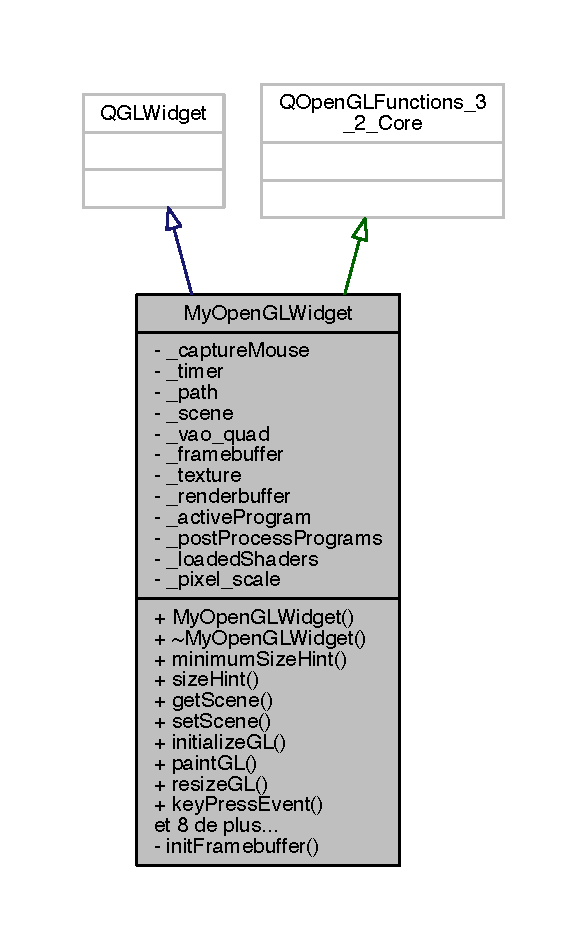
\includegraphics[width=282pt]{class_my_open_g_l_widget__inherit__graph}
\end{center}
\end{figure}


Graphe de collaboration de My\+Open\+G\+L\+Widget\+:
\nopagebreak
\begin{figure}[H]
\begin{center}
\leavevmode
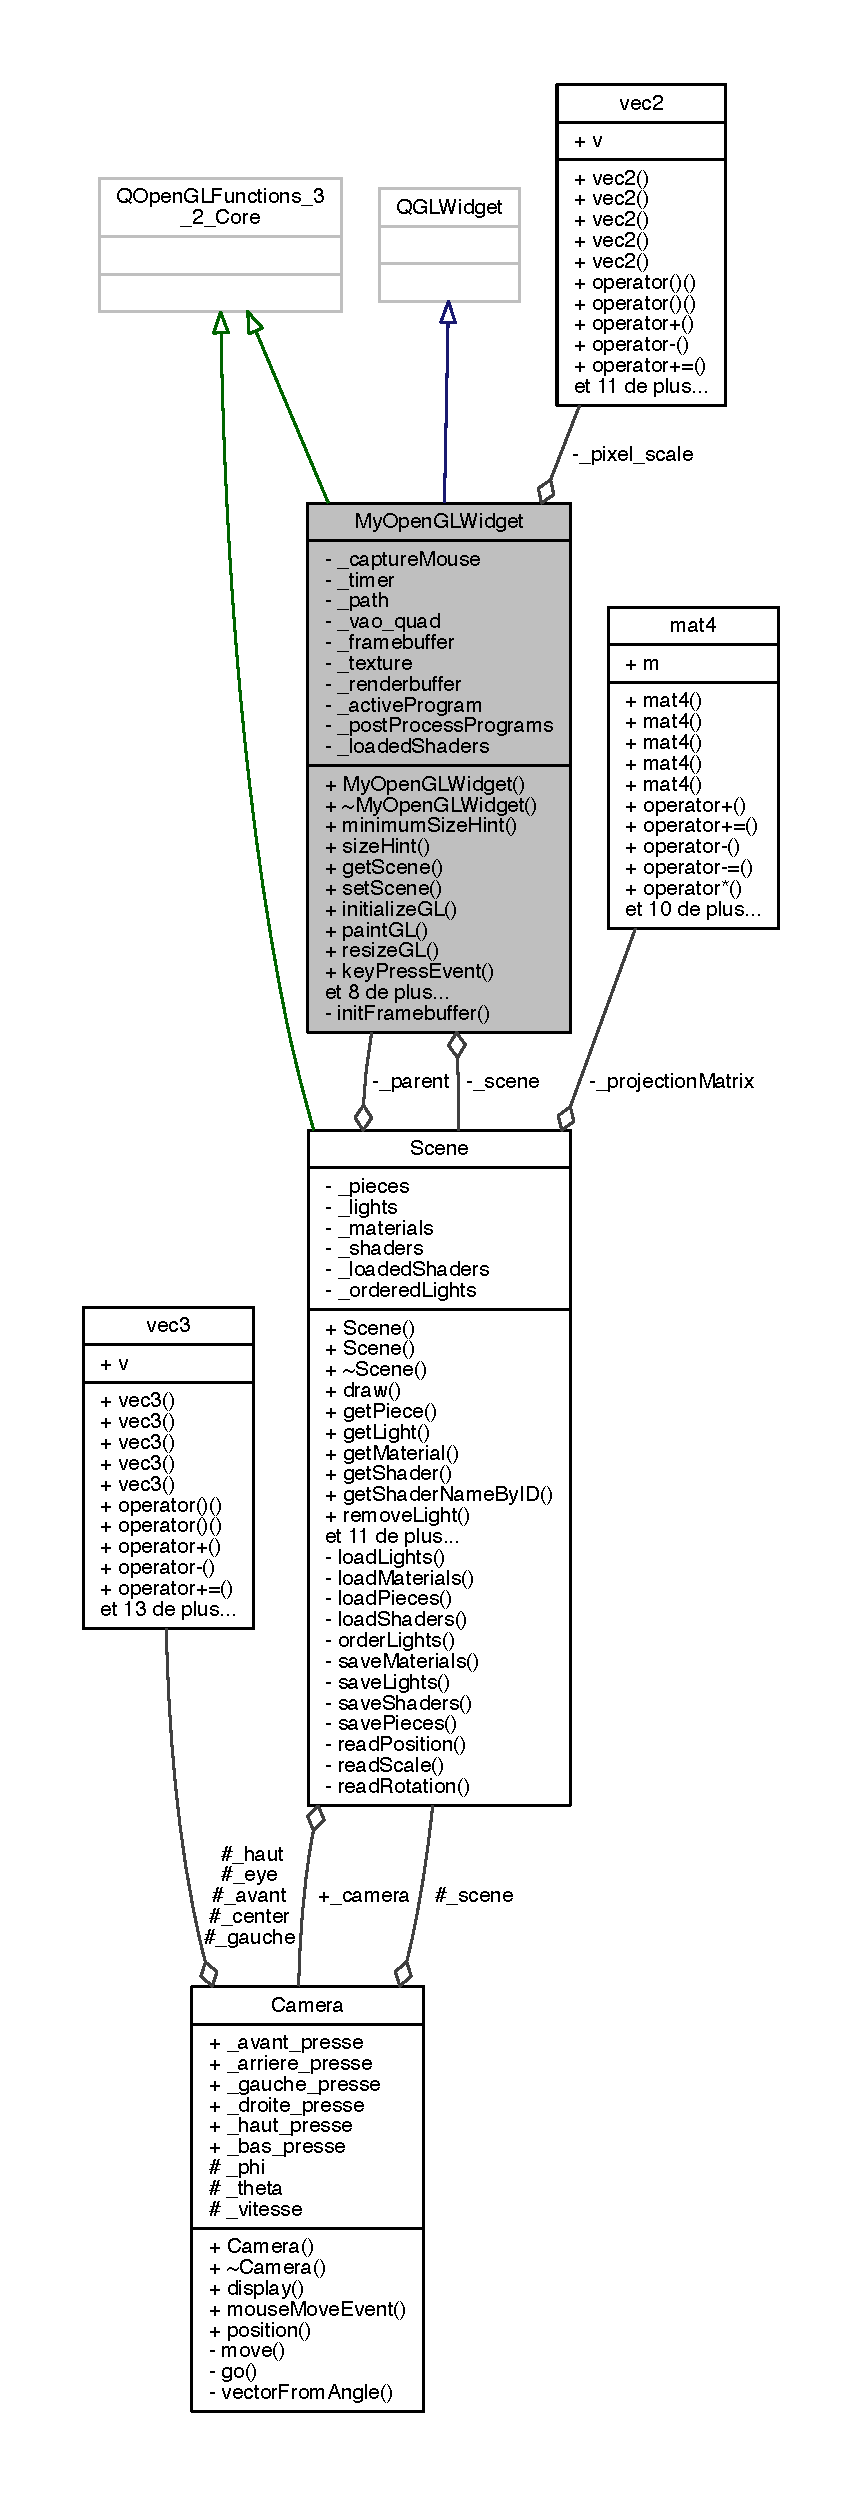
\includegraphics[height=550pt]{class_my_open_g_l_widget__coll__graph}
\end{center}
\end{figure}
\subsection*{Fonctions membres publiques}
\begin{DoxyCompactItemize}
\item 
\hyperlink{class_my_open_g_l_widget_a78f2284f348e8b482875ccdfbf704b34}{My\+Open\+G\+L\+Widget} (const Q\+G\+L\+Format \&format, Q\+Widget $\ast$parent=0, const Q\+String \&path=\char`\"{}\char`\"{}, const Q\+G\+L\+Widget $\ast$share\+Widget=0, Qt\+::\+Window\+Flags f=0)
\item 
\hyperlink{class_my_open_g_l_widget_aa9bdb4eb867d9e0bbfab210732fa5883}{$\sim$\+My\+Open\+G\+L\+Widget} ()
\item 
Q\+Size \hyperlink{class_my_open_g_l_widget_a4a037578f8e21a015e7b2915992fbe5d}{minimum\+Size\+Hint} () const 
\item 
Q\+Size \hyperlink{class_my_open_g_l_widget_abacca5d710f6a81b5edfd164f0148ed6}{size\+Hint} () const 
\item 
\hyperlink{class_scene}{Scene} $\ast$ \hyperlink{class_my_open_g_l_widget_ab25f238721b8e1cba36c2a0350ac57ba}{get\+Scene} ()
\item 
void \hyperlink{class_my_open_g_l_widget_aaac5737e9ce05a94006aa92afed5d403}{set\+Scene} (\hyperlink{class_scene}{Scene} $\ast$scene)
\item 
virtual void \hyperlink{class_my_open_g_l_widget_a98597f5669cec1c90f36c1d38569afc5}{initialize\+G\+L} ()
\item 
virtual void \hyperlink{class_my_open_g_l_widget_af7babfe769e968c317e646c4387b357d}{paint\+G\+L} ()
\item 
virtual void \hyperlink{class_my_open_g_l_widget_a51847d078dbd11fb99335abbc5eaf4fc}{resize\+G\+L} (int width, int height)
\item 
virtual void \hyperlink{class_my_open_g_l_widget_a87a479700547c066721b4b3532b040a2}{key\+Press\+Event} (Q\+Key\+Event $\ast$event)
\item 
virtual void \hyperlink{class_my_open_g_l_widget_a57e054ac1c21ed8585ca57b151ec6b38}{key\+Release\+Event} (Q\+Key\+Event $\ast$event)
\item 
virtual void \hyperlink{class_my_open_g_l_widget_a27abe02c04240317cf42c1cec1ac7e25}{mouse\+Move\+Event} (Q\+Mouse\+Event $\ast$event)
\item 
virtual void \hyperlink{class_my_open_g_l_widget_a6a2e229f91bb75775bb539c85bb696ef}{mouse\+Press\+Event} (Q\+Mouse\+Event $\ast$event)
\item 
void \hyperlink{class_my_open_g_l_widget_a87b9f933f545bf6f257820395771cc8b}{use\+Shader} (const Q\+String \&name)
\item 
void \hyperlink{class_my_open_g_l_widget_a1426e6f24592838e16c22a92870cf5f4}{add\+Shader} (const Q\+String \&name, const Q\+String \&vertex, const Q\+String \&fragment)
\item 
Q\+String\+List \hyperlink{class_my_open_g_l_widget_a99929e3c743d4f5793ef0e09ab61f2b2}{get\+Shader\+Names} ()
\item 
void \hyperlink{class_my_open_g_l_widget_af7899fd91898c1ed5dc228d7d6de658e}{load\+Shaders} (const Q\+Dom\+Element \&post\+Process)
\item 
void \hyperlink{class_my_open_g_l_widget_a177cfabda79d05c834b4f1a3f370a620}{save\+Shaders} (Q\+Dom\+Element \&root, Q\+Dom\+Document \&doc) const 
\end{DoxyCompactItemize}
\subsection*{Fonctions membres privées}
\begin{DoxyCompactItemize}
\item 
void \hyperlink{class_my_open_g_l_widget_ae2bcca23e0802d6f5ebf2ee3e6ed6e7a}{init\+Framebuffer} (int width, int height)
\end{DoxyCompactItemize}
\subsection*{Attributs privés}
\begin{DoxyCompactItemize}
\item 
bool \hyperlink{class_my_open_g_l_widget_af001d889fec5469aa3e67c11ae48b29d}{\+\_\+capture\+Mouse}
\item 
Q\+Timer $\ast$ \hyperlink{class_my_open_g_l_widget_aa6ba509f0ef6e8c2d266b83e1d380eb8}{\+\_\+timer}
\item 
Q\+String \hyperlink{class_my_open_g_l_widget_a7b3d69ddf0b3509a196edbfeb78407c6}{\+\_\+path}
\item 
\hyperlink{class_scene}{Scene} $\ast$ \hyperlink{class_my_open_g_l_widget_a26a1f259357dd7c8822d715d81591395}{\+\_\+scene}
\item 
G\+Luint \hyperlink{class_my_open_g_l_widget_a63a814817d1af6ea49036edac108183b}{\+\_\+vao\+\_\+quad}
\item 
G\+Luint \hyperlink{class_my_open_g_l_widget_ab39ecf367a98c1bd5e1dbeeb8b44a255}{\+\_\+framebuffer}
\item 
G\+Luint \hyperlink{class_my_open_g_l_widget_a18d7f106f5e12568f5db59d8c4a71706}{\+\_\+texture}
\item 
G\+Luint \hyperlink{class_my_open_g_l_widget_a8385a49fb5113010acc3ddd67080ed1a}{\+\_\+renderbuffer}
\item 
Q\+Open\+G\+L\+Shader\+Program $\ast$ \hyperlink{class_my_open_g_l_widget_a24571f61604a92b622b49609bc0f3f5b}{\+\_\+active\+Program}
\item 
Q\+Map$<$ Q\+String, \\*
Q\+Open\+G\+L\+Shader\+Program $\ast$ $>$ \hyperlink{class_my_open_g_l_widget_afde13326f4f01ede3cac0ee4f389a594}{\+\_\+post\+Process\+Programs}
\item 
Q\+Map$<$ Q\+String, Q\+Open\+G\+L\+Shader $\ast$ $>$ \hyperlink{class_my_open_g_l_widget_ab02762bc0b4cb541f7ad42fdbd7a73f7}{\+\_\+loaded\+Shaders}
\item 
\hyperlink{structvec2}{vec2} \hyperlink{class_my_open_g_l_widget_a543e9cc55491a8e07a7bb5eb54633351}{\+\_\+pixel\+\_\+scale}
\end{DoxyCompactItemize}


\subsection{Documentation des constructeurs et destructeur}
\hypertarget{class_my_open_g_l_widget_a78f2284f348e8b482875ccdfbf704b34}{\index{My\+Open\+G\+L\+Widget@{My\+Open\+G\+L\+Widget}!My\+Open\+G\+L\+Widget@{My\+Open\+G\+L\+Widget}}
\index{My\+Open\+G\+L\+Widget@{My\+Open\+G\+L\+Widget}!My\+Open\+G\+L\+Widget@{My\+Open\+G\+L\+Widget}}
\subsubsection[{My\+Open\+G\+L\+Widget}]{\setlength{\rightskip}{0pt plus 5cm}My\+Open\+G\+L\+Widget\+::\+My\+Open\+G\+L\+Widget (
\begin{DoxyParamCaption}
\item[{const Q\+G\+L\+Format \&}]{format, }
\item[{Q\+Widget $\ast$}]{parent = {\ttfamily 0}, }
\item[{const Q\+String \&}]{path = {\ttfamily \char`\"{}\char`\"{}}, }
\item[{const Q\+G\+L\+Widget $\ast$}]{share\+Widget = {\ttfamily 0}, }
\item[{Qt\+::\+Window\+Flags}]{f = {\ttfamily 0}}
\end{DoxyParamCaption}
)}}\label{class_my_open_g_l_widget_a78f2284f348e8b482875ccdfbf704b34}
\hypertarget{class_my_open_g_l_widget_aa9bdb4eb867d9e0bbfab210732fa5883}{\index{My\+Open\+G\+L\+Widget@{My\+Open\+G\+L\+Widget}!````~My\+Open\+G\+L\+Widget@{$\sim$\+My\+Open\+G\+L\+Widget}}
\index{````~My\+Open\+G\+L\+Widget@{$\sim$\+My\+Open\+G\+L\+Widget}!My\+Open\+G\+L\+Widget@{My\+Open\+G\+L\+Widget}}
\subsubsection[{$\sim$\+My\+Open\+G\+L\+Widget}]{\setlength{\rightskip}{0pt plus 5cm}My\+Open\+G\+L\+Widget\+::$\sim$\+My\+Open\+G\+L\+Widget (
\begin{DoxyParamCaption}
{}
\end{DoxyParamCaption}
)}}\label{class_my_open_g_l_widget_aa9bdb4eb867d9e0bbfab210732fa5883}


\subsection{Documentation des fonctions membres}
\hypertarget{class_my_open_g_l_widget_a1426e6f24592838e16c22a92870cf5f4}{\index{My\+Open\+G\+L\+Widget@{My\+Open\+G\+L\+Widget}!add\+Shader@{add\+Shader}}
\index{add\+Shader@{add\+Shader}!My\+Open\+G\+L\+Widget@{My\+Open\+G\+L\+Widget}}
\subsubsection[{add\+Shader}]{\setlength{\rightskip}{0pt plus 5cm}void My\+Open\+G\+L\+Widget\+::add\+Shader (
\begin{DoxyParamCaption}
\item[{const Q\+String \&}]{name, }
\item[{const Q\+String \&}]{vertex, }
\item[{const Q\+String \&}]{fragment}
\end{DoxyParamCaption}
)}}\label{class_my_open_g_l_widget_a1426e6f24592838e16c22a92870cf5f4}


Voici le graphe des appelants de cette fonction \+:
\nopagebreak
\begin{figure}[H]
\begin{center}
\leavevmode
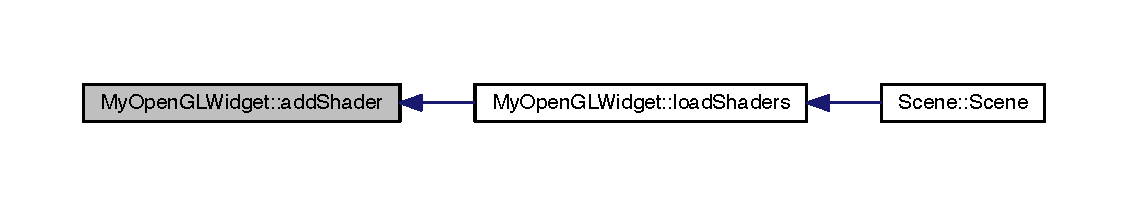
\includegraphics[width=350pt]{class_my_open_g_l_widget_a1426e6f24592838e16c22a92870cf5f4_icgraph}
\end{center}
\end{figure}


\hypertarget{class_my_open_g_l_widget_ab25f238721b8e1cba36c2a0350ac57ba}{\index{My\+Open\+G\+L\+Widget@{My\+Open\+G\+L\+Widget}!get\+Scene@{get\+Scene}}
\index{get\+Scene@{get\+Scene}!My\+Open\+G\+L\+Widget@{My\+Open\+G\+L\+Widget}}
\subsubsection[{get\+Scene}]{\setlength{\rightskip}{0pt plus 5cm}{\bf Scene} $\ast$ My\+Open\+G\+L\+Widget\+::get\+Scene (
\begin{DoxyParamCaption}
{}
\end{DoxyParamCaption}
)}}\label{class_my_open_g_l_widget_ab25f238721b8e1cba36c2a0350ac57ba}


Voici le graphe des appelants de cette fonction \+:
\nopagebreak
\begin{figure}[H]
\begin{center}
\leavevmode
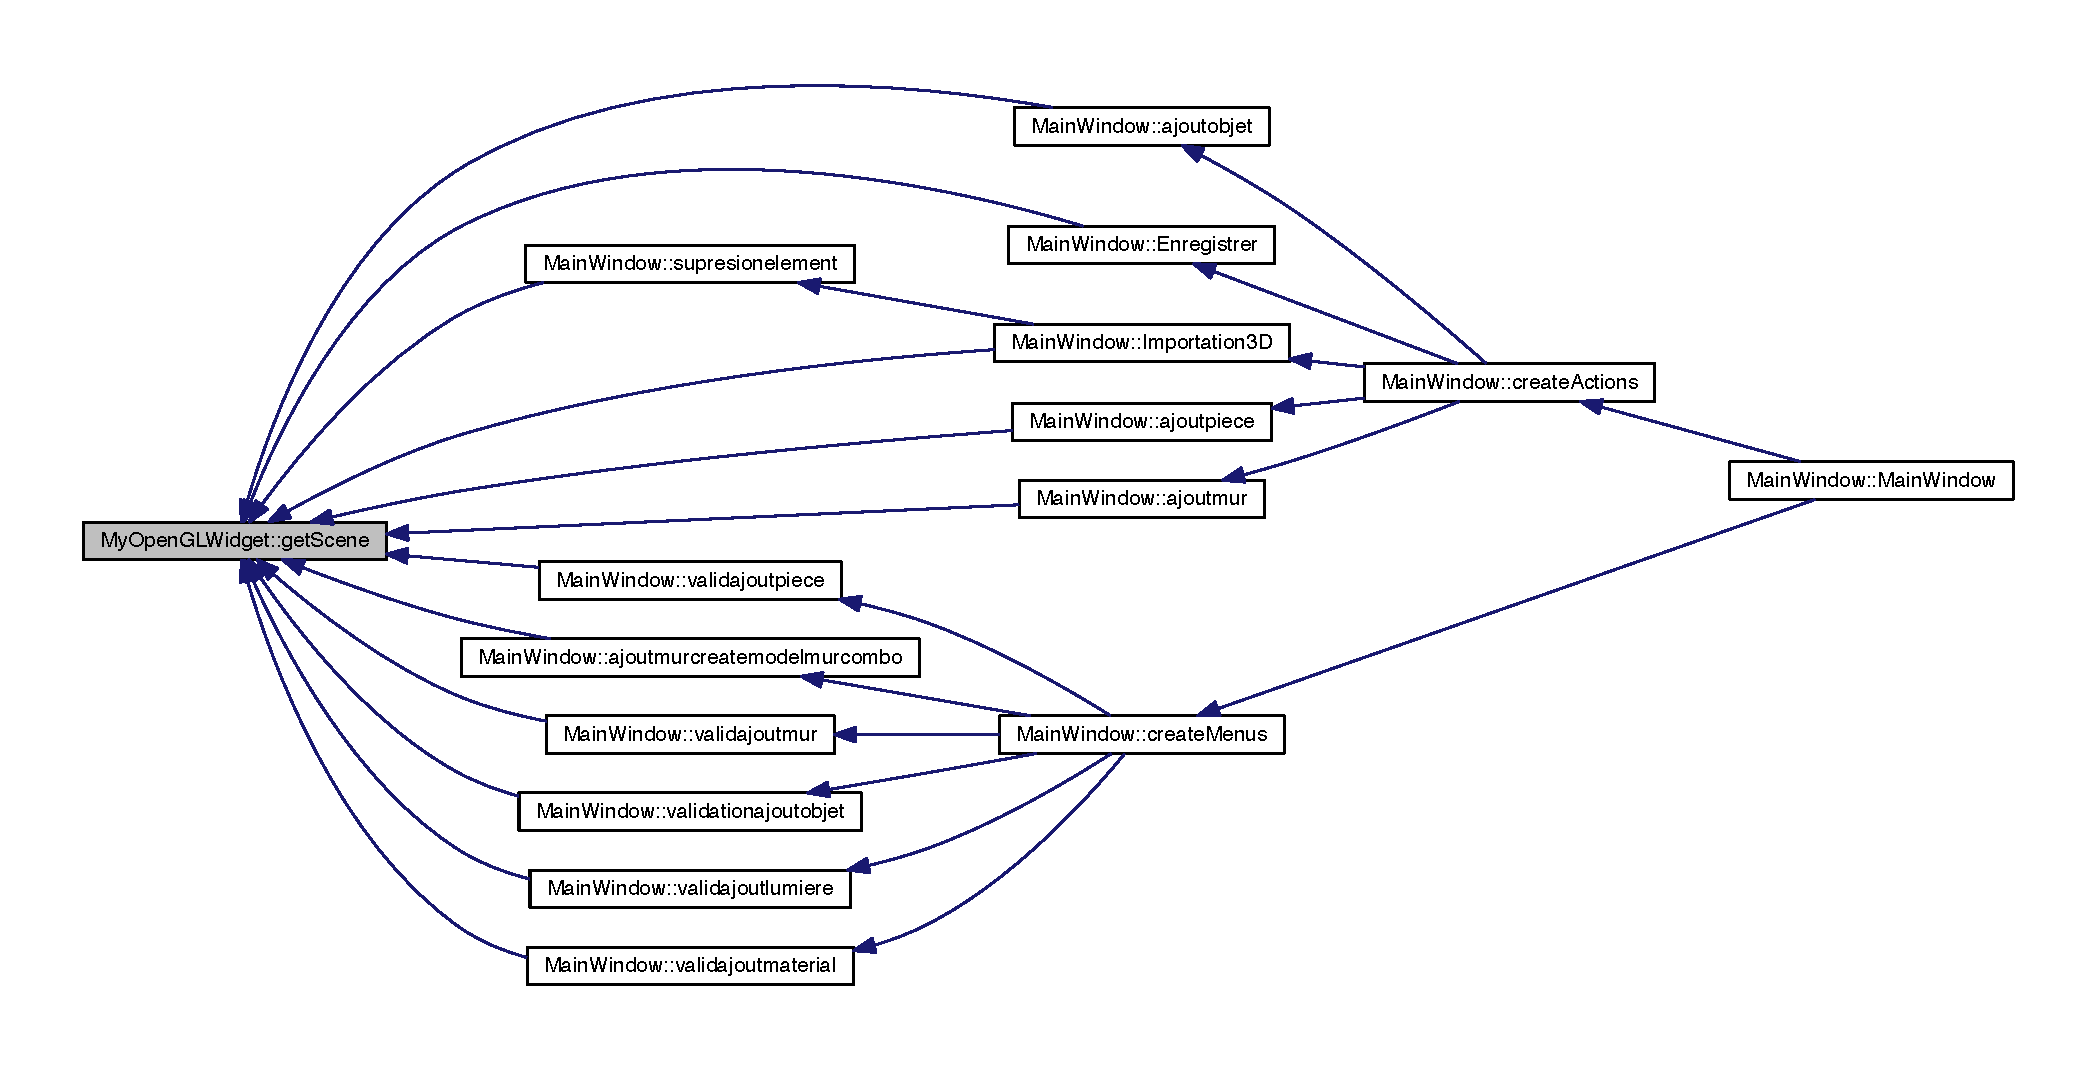
\includegraphics[width=350pt]{class_my_open_g_l_widget_ab25f238721b8e1cba36c2a0350ac57ba_icgraph}
\end{center}
\end{figure}


\hypertarget{class_my_open_g_l_widget_a99929e3c743d4f5793ef0e09ab61f2b2}{\index{My\+Open\+G\+L\+Widget@{My\+Open\+G\+L\+Widget}!get\+Shader\+Names@{get\+Shader\+Names}}
\index{get\+Shader\+Names@{get\+Shader\+Names}!My\+Open\+G\+L\+Widget@{My\+Open\+G\+L\+Widget}}
\subsubsection[{get\+Shader\+Names}]{\setlength{\rightskip}{0pt plus 5cm}Q\+String\+List My\+Open\+G\+L\+Widget\+::get\+Shader\+Names (
\begin{DoxyParamCaption}
{}
\end{DoxyParamCaption}
)}}\label{class_my_open_g_l_widget_a99929e3c743d4f5793ef0e09ab61f2b2}


Voici le graphe des appelants de cette fonction \+:
\nopagebreak
\begin{figure}[H]
\begin{center}
\leavevmode
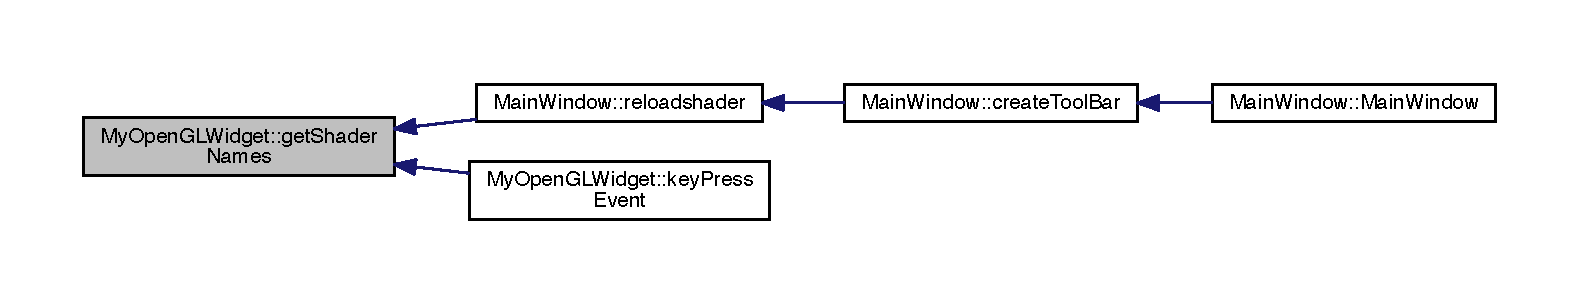
\includegraphics[width=350pt]{class_my_open_g_l_widget_a99929e3c743d4f5793ef0e09ab61f2b2_icgraph}
\end{center}
\end{figure}


\hypertarget{class_my_open_g_l_widget_ae2bcca23e0802d6f5ebf2ee3e6ed6e7a}{\index{My\+Open\+G\+L\+Widget@{My\+Open\+G\+L\+Widget}!init\+Framebuffer@{init\+Framebuffer}}
\index{init\+Framebuffer@{init\+Framebuffer}!My\+Open\+G\+L\+Widget@{My\+Open\+G\+L\+Widget}}
\subsubsection[{init\+Framebuffer}]{\setlength{\rightskip}{0pt plus 5cm}void My\+Open\+G\+L\+Widget\+::init\+Framebuffer (
\begin{DoxyParamCaption}
\item[{int}]{width, }
\item[{int}]{height}
\end{DoxyParamCaption}
)\hspace{0.3cm}{\ttfamily [private]}}}\label{class_my_open_g_l_widget_ae2bcca23e0802d6f5ebf2ee3e6ed6e7a}


Voici le graphe des appelants de cette fonction \+:
\nopagebreak
\begin{figure}[H]
\begin{center}
\leavevmode
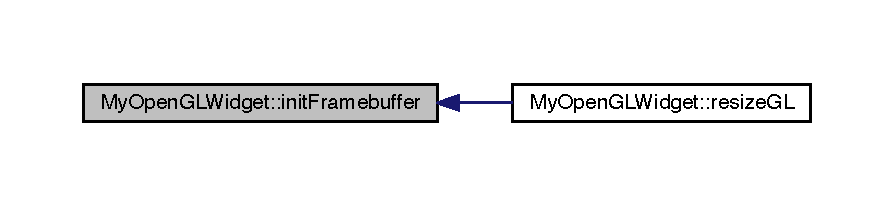
\includegraphics[width=350pt]{class_my_open_g_l_widget_ae2bcca23e0802d6f5ebf2ee3e6ed6e7a_icgraph}
\end{center}
\end{figure}


\hypertarget{class_my_open_g_l_widget_a98597f5669cec1c90f36c1d38569afc5}{\index{My\+Open\+G\+L\+Widget@{My\+Open\+G\+L\+Widget}!initialize\+G\+L@{initialize\+G\+L}}
\index{initialize\+G\+L@{initialize\+G\+L}!My\+Open\+G\+L\+Widget@{My\+Open\+G\+L\+Widget}}
\subsubsection[{initialize\+G\+L}]{\setlength{\rightskip}{0pt plus 5cm}void My\+Open\+G\+L\+Widget\+::initialize\+G\+L (
\begin{DoxyParamCaption}
{}
\end{DoxyParamCaption}
)\hspace{0.3cm}{\ttfamily [virtual]}}}\label{class_my_open_g_l_widget_a98597f5669cec1c90f36c1d38569afc5}
\hypertarget{class_my_open_g_l_widget_a87a479700547c066721b4b3532b040a2}{\index{My\+Open\+G\+L\+Widget@{My\+Open\+G\+L\+Widget}!key\+Press\+Event@{key\+Press\+Event}}
\index{key\+Press\+Event@{key\+Press\+Event}!My\+Open\+G\+L\+Widget@{My\+Open\+G\+L\+Widget}}
\subsubsection[{key\+Press\+Event}]{\setlength{\rightskip}{0pt plus 5cm}void My\+Open\+G\+L\+Widget\+::key\+Press\+Event (
\begin{DoxyParamCaption}
\item[{Q\+Key\+Event $\ast$}]{event}
\end{DoxyParamCaption}
)\hspace{0.3cm}{\ttfamily [virtual]}}}\label{class_my_open_g_l_widget_a87a479700547c066721b4b3532b040a2}


Voici le graphe d'appel pour cette fonction \+:
\nopagebreak
\begin{figure}[H]
\begin{center}
\leavevmode
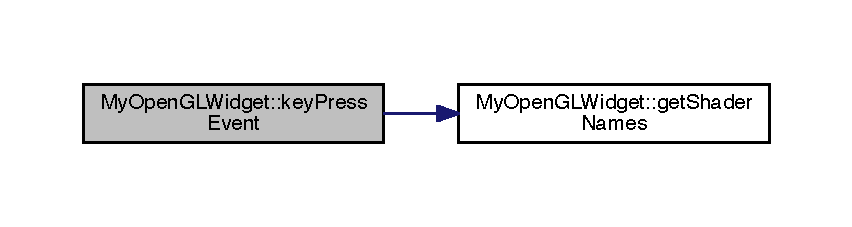
\includegraphics[width=350pt]{class_my_open_g_l_widget_a87a479700547c066721b4b3532b040a2_cgraph}
\end{center}
\end{figure}


\hypertarget{class_my_open_g_l_widget_a57e054ac1c21ed8585ca57b151ec6b38}{\index{My\+Open\+G\+L\+Widget@{My\+Open\+G\+L\+Widget}!key\+Release\+Event@{key\+Release\+Event}}
\index{key\+Release\+Event@{key\+Release\+Event}!My\+Open\+G\+L\+Widget@{My\+Open\+G\+L\+Widget}}
\subsubsection[{key\+Release\+Event}]{\setlength{\rightskip}{0pt plus 5cm}void My\+Open\+G\+L\+Widget\+::key\+Release\+Event (
\begin{DoxyParamCaption}
\item[{Q\+Key\+Event $\ast$}]{event}
\end{DoxyParamCaption}
)\hspace{0.3cm}{\ttfamily [virtual]}}}\label{class_my_open_g_l_widget_a57e054ac1c21ed8585ca57b151ec6b38}
\hypertarget{class_my_open_g_l_widget_af7899fd91898c1ed5dc228d7d6de658e}{\index{My\+Open\+G\+L\+Widget@{My\+Open\+G\+L\+Widget}!load\+Shaders@{load\+Shaders}}
\index{load\+Shaders@{load\+Shaders}!My\+Open\+G\+L\+Widget@{My\+Open\+G\+L\+Widget}}
\subsubsection[{load\+Shaders}]{\setlength{\rightskip}{0pt plus 5cm}void My\+Open\+G\+L\+Widget\+::load\+Shaders (
\begin{DoxyParamCaption}
\item[{const Q\+Dom\+Element \&}]{post\+Process}
\end{DoxyParamCaption}
)}}\label{class_my_open_g_l_widget_af7899fd91898c1ed5dc228d7d6de658e}


Voici le graphe d'appel pour cette fonction \+:
\nopagebreak
\begin{figure}[H]
\begin{center}
\leavevmode
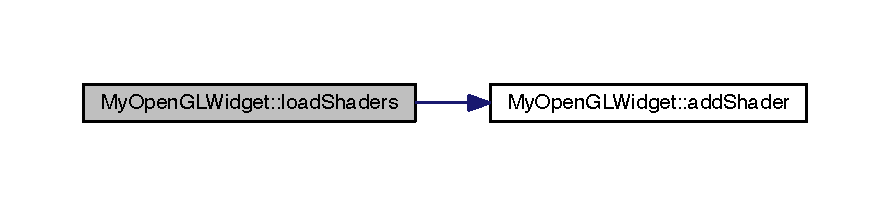
\includegraphics[width=350pt]{class_my_open_g_l_widget_af7899fd91898c1ed5dc228d7d6de658e_cgraph}
\end{center}
\end{figure}




Voici le graphe des appelants de cette fonction \+:
\nopagebreak
\begin{figure}[H]
\begin{center}
\leavevmode
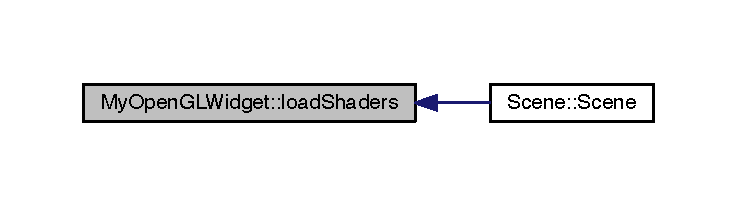
\includegraphics[width=350pt]{class_my_open_g_l_widget_af7899fd91898c1ed5dc228d7d6de658e_icgraph}
\end{center}
\end{figure}


\hypertarget{class_my_open_g_l_widget_a4a037578f8e21a015e7b2915992fbe5d}{\index{My\+Open\+G\+L\+Widget@{My\+Open\+G\+L\+Widget}!minimum\+Size\+Hint@{minimum\+Size\+Hint}}
\index{minimum\+Size\+Hint@{minimum\+Size\+Hint}!My\+Open\+G\+L\+Widget@{My\+Open\+G\+L\+Widget}}
\subsubsection[{minimum\+Size\+Hint}]{\setlength{\rightskip}{0pt plus 5cm}Q\+Size My\+Open\+G\+L\+Widget\+::minimum\+Size\+Hint (
\begin{DoxyParamCaption}
{}
\end{DoxyParamCaption}
) const}}\label{class_my_open_g_l_widget_a4a037578f8e21a015e7b2915992fbe5d}
\hypertarget{class_my_open_g_l_widget_a27abe02c04240317cf42c1cec1ac7e25}{\index{My\+Open\+G\+L\+Widget@{My\+Open\+G\+L\+Widget}!mouse\+Move\+Event@{mouse\+Move\+Event}}
\index{mouse\+Move\+Event@{mouse\+Move\+Event}!My\+Open\+G\+L\+Widget@{My\+Open\+G\+L\+Widget}}
\subsubsection[{mouse\+Move\+Event}]{\setlength{\rightskip}{0pt plus 5cm}void My\+Open\+G\+L\+Widget\+::mouse\+Move\+Event (
\begin{DoxyParamCaption}
\item[{Q\+Mouse\+Event $\ast$}]{event}
\end{DoxyParamCaption}
)\hspace{0.3cm}{\ttfamily [virtual]}}}\label{class_my_open_g_l_widget_a27abe02c04240317cf42c1cec1ac7e25}


Voici le graphe d'appel pour cette fonction \+:
\nopagebreak
\begin{figure}[H]
\begin{center}
\leavevmode
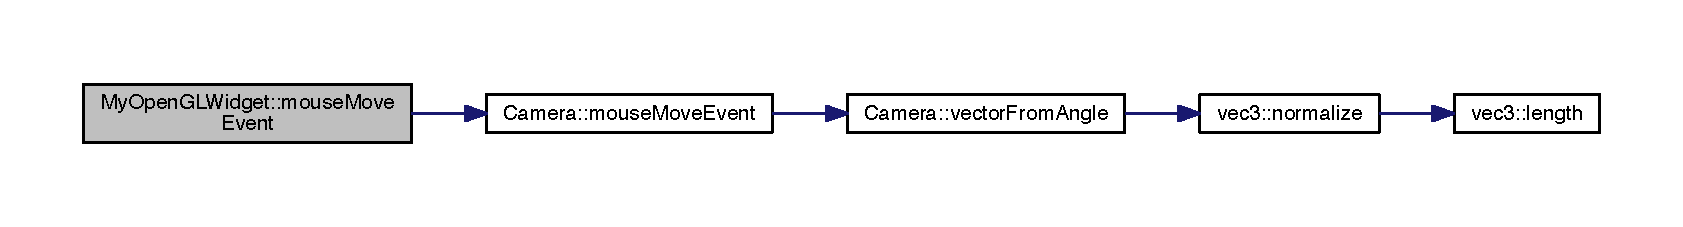
\includegraphics[width=350pt]{class_my_open_g_l_widget_a27abe02c04240317cf42c1cec1ac7e25_cgraph}
\end{center}
\end{figure}


\hypertarget{class_my_open_g_l_widget_a6a2e229f91bb75775bb539c85bb696ef}{\index{My\+Open\+G\+L\+Widget@{My\+Open\+G\+L\+Widget}!mouse\+Press\+Event@{mouse\+Press\+Event}}
\index{mouse\+Press\+Event@{mouse\+Press\+Event}!My\+Open\+G\+L\+Widget@{My\+Open\+G\+L\+Widget}}
\subsubsection[{mouse\+Press\+Event}]{\setlength{\rightskip}{0pt plus 5cm}void My\+Open\+G\+L\+Widget\+::mouse\+Press\+Event (
\begin{DoxyParamCaption}
\item[{Q\+Mouse\+Event $\ast$}]{event}
\end{DoxyParamCaption}
)\hspace{0.3cm}{\ttfamily [virtual]}}}\label{class_my_open_g_l_widget_a6a2e229f91bb75775bb539c85bb696ef}
\hypertarget{class_my_open_g_l_widget_af7babfe769e968c317e646c4387b357d}{\index{My\+Open\+G\+L\+Widget@{My\+Open\+G\+L\+Widget}!paint\+G\+L@{paint\+G\+L}}
\index{paint\+G\+L@{paint\+G\+L}!My\+Open\+G\+L\+Widget@{My\+Open\+G\+L\+Widget}}
\subsubsection[{paint\+G\+L}]{\setlength{\rightskip}{0pt plus 5cm}void My\+Open\+G\+L\+Widget\+::paint\+G\+L (
\begin{DoxyParamCaption}
{}
\end{DoxyParamCaption}
)\hspace{0.3cm}{\ttfamily [virtual]}}}\label{class_my_open_g_l_widget_af7babfe769e968c317e646c4387b357d}


Voici le graphe d'appel pour cette fonction \+:
\nopagebreak
\begin{figure}[H]
\begin{center}
\leavevmode
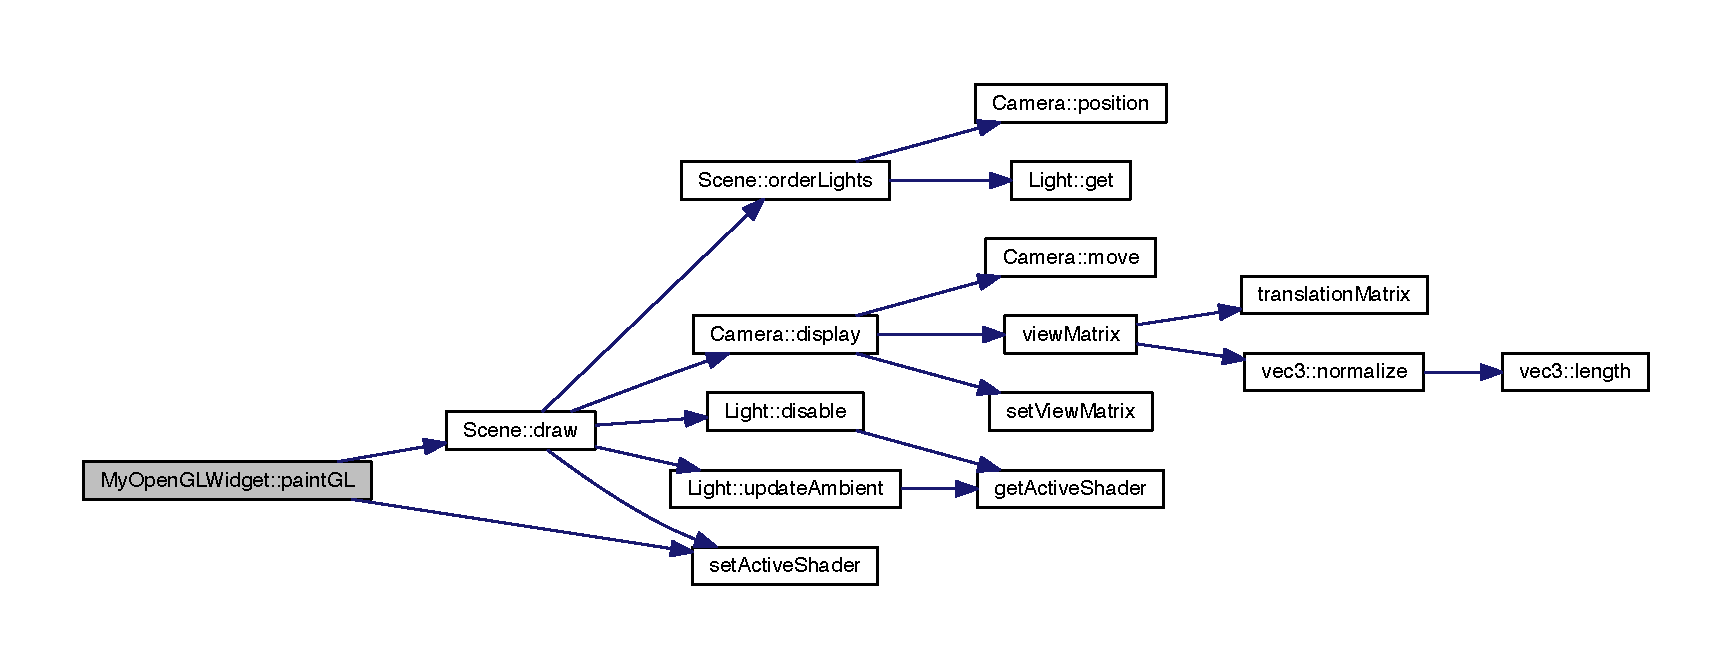
\includegraphics[width=350pt]{class_my_open_g_l_widget_af7babfe769e968c317e646c4387b357d_cgraph}
\end{center}
\end{figure}


\hypertarget{class_my_open_g_l_widget_a51847d078dbd11fb99335abbc5eaf4fc}{\index{My\+Open\+G\+L\+Widget@{My\+Open\+G\+L\+Widget}!resize\+G\+L@{resize\+G\+L}}
\index{resize\+G\+L@{resize\+G\+L}!My\+Open\+G\+L\+Widget@{My\+Open\+G\+L\+Widget}}
\subsubsection[{resize\+G\+L}]{\setlength{\rightskip}{0pt plus 5cm}void My\+Open\+G\+L\+Widget\+::resize\+G\+L (
\begin{DoxyParamCaption}
\item[{int}]{width, }
\item[{int}]{height}
\end{DoxyParamCaption}
)\hspace{0.3cm}{\ttfamily [virtual]}}}\label{class_my_open_g_l_widget_a51847d078dbd11fb99335abbc5eaf4fc}


Voici le graphe d'appel pour cette fonction \+:
\nopagebreak
\begin{figure}[H]
\begin{center}
\leavevmode
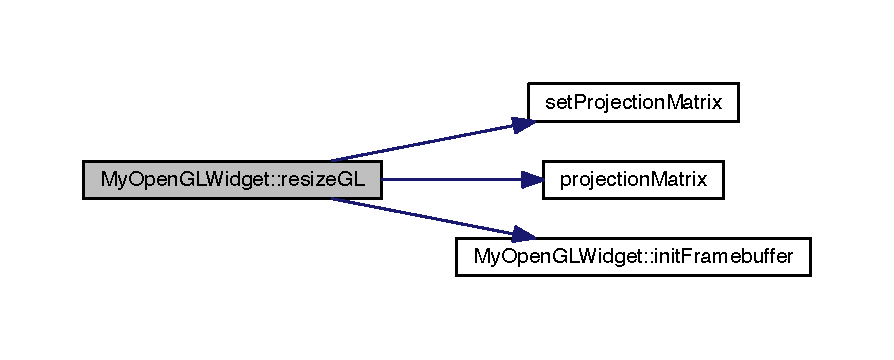
\includegraphics[width=350pt]{class_my_open_g_l_widget_a51847d078dbd11fb99335abbc5eaf4fc_cgraph}
\end{center}
\end{figure}


\hypertarget{class_my_open_g_l_widget_a177cfabda79d05c834b4f1a3f370a620}{\index{My\+Open\+G\+L\+Widget@{My\+Open\+G\+L\+Widget}!save\+Shaders@{save\+Shaders}}
\index{save\+Shaders@{save\+Shaders}!My\+Open\+G\+L\+Widget@{My\+Open\+G\+L\+Widget}}
\subsubsection[{save\+Shaders}]{\setlength{\rightskip}{0pt plus 5cm}void My\+Open\+G\+L\+Widget\+::save\+Shaders (
\begin{DoxyParamCaption}
\item[{Q\+Dom\+Element \&}]{root, }
\item[{Q\+Dom\+Document \&}]{doc}
\end{DoxyParamCaption}
) const}}\label{class_my_open_g_l_widget_a177cfabda79d05c834b4f1a3f370a620}


Voici le graphe des appelants de cette fonction \+:
\nopagebreak
\begin{figure}[H]
\begin{center}
\leavevmode
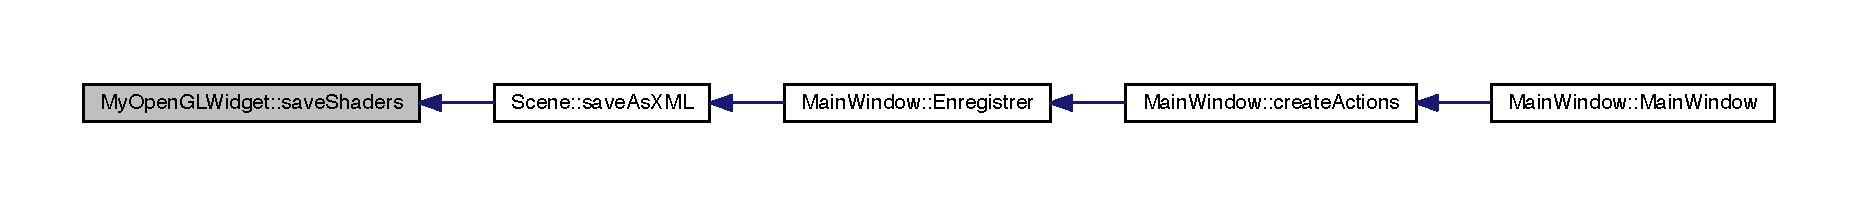
\includegraphics[width=350pt]{class_my_open_g_l_widget_a177cfabda79d05c834b4f1a3f370a620_icgraph}
\end{center}
\end{figure}


\hypertarget{class_my_open_g_l_widget_aaac5737e9ce05a94006aa92afed5d403}{\index{My\+Open\+G\+L\+Widget@{My\+Open\+G\+L\+Widget}!set\+Scene@{set\+Scene}}
\index{set\+Scene@{set\+Scene}!My\+Open\+G\+L\+Widget@{My\+Open\+G\+L\+Widget}}
\subsubsection[{set\+Scene}]{\setlength{\rightskip}{0pt plus 5cm}void My\+Open\+G\+L\+Widget\+::set\+Scene (
\begin{DoxyParamCaption}
\item[{{\bf Scene} $\ast$}]{scene}
\end{DoxyParamCaption}
)}}\label{class_my_open_g_l_widget_aaac5737e9ce05a94006aa92afed5d403}
\hypertarget{class_my_open_g_l_widget_abacca5d710f6a81b5edfd164f0148ed6}{\index{My\+Open\+G\+L\+Widget@{My\+Open\+G\+L\+Widget}!size\+Hint@{size\+Hint}}
\index{size\+Hint@{size\+Hint}!My\+Open\+G\+L\+Widget@{My\+Open\+G\+L\+Widget}}
\subsubsection[{size\+Hint}]{\setlength{\rightskip}{0pt plus 5cm}Q\+Size My\+Open\+G\+L\+Widget\+::size\+Hint (
\begin{DoxyParamCaption}
{}
\end{DoxyParamCaption}
) const}}\label{class_my_open_g_l_widget_abacca5d710f6a81b5edfd164f0148ed6}
\hypertarget{class_my_open_g_l_widget_a87b9f933f545bf6f257820395771cc8b}{\index{My\+Open\+G\+L\+Widget@{My\+Open\+G\+L\+Widget}!use\+Shader@{use\+Shader}}
\index{use\+Shader@{use\+Shader}!My\+Open\+G\+L\+Widget@{My\+Open\+G\+L\+Widget}}
\subsubsection[{use\+Shader}]{\setlength{\rightskip}{0pt plus 5cm}void My\+Open\+G\+L\+Widget\+::use\+Shader (
\begin{DoxyParamCaption}
\item[{const Q\+String \&}]{name}
\end{DoxyParamCaption}
)}}\label{class_my_open_g_l_widget_a87b9f933f545bf6f257820395771cc8b}


Voici le graphe des appelants de cette fonction \+:
\nopagebreak
\begin{figure}[H]
\begin{center}
\leavevmode
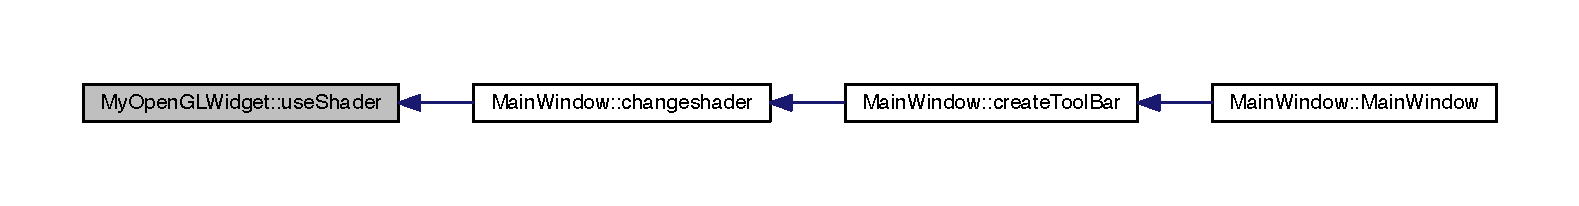
\includegraphics[width=350pt]{class_my_open_g_l_widget_a87b9f933f545bf6f257820395771cc8b_icgraph}
\end{center}
\end{figure}




\subsection{Documentation des données membres}
\hypertarget{class_my_open_g_l_widget_a24571f61604a92b622b49609bc0f3f5b}{\index{My\+Open\+G\+L\+Widget@{My\+Open\+G\+L\+Widget}!\+\_\+active\+Program@{\+\_\+active\+Program}}
\index{\+\_\+active\+Program@{\+\_\+active\+Program}!My\+Open\+G\+L\+Widget@{My\+Open\+G\+L\+Widget}}
\subsubsection[{\+\_\+active\+Program}]{\setlength{\rightskip}{0pt plus 5cm}Q\+Open\+G\+L\+Shader\+Program$\ast$ My\+Open\+G\+L\+Widget\+::\+\_\+active\+Program\hspace{0.3cm}{\ttfamily [private]}}}\label{class_my_open_g_l_widget_a24571f61604a92b622b49609bc0f3f5b}
\hypertarget{class_my_open_g_l_widget_af001d889fec5469aa3e67c11ae48b29d}{\index{My\+Open\+G\+L\+Widget@{My\+Open\+G\+L\+Widget}!\+\_\+capture\+Mouse@{\+\_\+capture\+Mouse}}
\index{\+\_\+capture\+Mouse@{\+\_\+capture\+Mouse}!My\+Open\+G\+L\+Widget@{My\+Open\+G\+L\+Widget}}
\subsubsection[{\+\_\+capture\+Mouse}]{\setlength{\rightskip}{0pt plus 5cm}bool My\+Open\+G\+L\+Widget\+::\+\_\+capture\+Mouse\hspace{0.3cm}{\ttfamily [private]}}}\label{class_my_open_g_l_widget_af001d889fec5469aa3e67c11ae48b29d}
\hypertarget{class_my_open_g_l_widget_ab39ecf367a98c1bd5e1dbeeb8b44a255}{\index{My\+Open\+G\+L\+Widget@{My\+Open\+G\+L\+Widget}!\+\_\+framebuffer@{\+\_\+framebuffer}}
\index{\+\_\+framebuffer@{\+\_\+framebuffer}!My\+Open\+G\+L\+Widget@{My\+Open\+G\+L\+Widget}}
\subsubsection[{\+\_\+framebuffer}]{\setlength{\rightskip}{0pt plus 5cm}G\+Luint My\+Open\+G\+L\+Widget\+::\+\_\+framebuffer\hspace{0.3cm}{\ttfamily [private]}}}\label{class_my_open_g_l_widget_ab39ecf367a98c1bd5e1dbeeb8b44a255}
\hypertarget{class_my_open_g_l_widget_ab02762bc0b4cb541f7ad42fdbd7a73f7}{\index{My\+Open\+G\+L\+Widget@{My\+Open\+G\+L\+Widget}!\+\_\+loaded\+Shaders@{\+\_\+loaded\+Shaders}}
\index{\+\_\+loaded\+Shaders@{\+\_\+loaded\+Shaders}!My\+Open\+G\+L\+Widget@{My\+Open\+G\+L\+Widget}}
\subsubsection[{\+\_\+loaded\+Shaders}]{\setlength{\rightskip}{0pt plus 5cm}Q\+Map$<$Q\+String, Q\+Open\+G\+L\+Shader $\ast$$>$ My\+Open\+G\+L\+Widget\+::\+\_\+loaded\+Shaders\hspace{0.3cm}{\ttfamily [private]}}}\label{class_my_open_g_l_widget_ab02762bc0b4cb541f7ad42fdbd7a73f7}
\hypertarget{class_my_open_g_l_widget_a7b3d69ddf0b3509a196edbfeb78407c6}{\index{My\+Open\+G\+L\+Widget@{My\+Open\+G\+L\+Widget}!\+\_\+path@{\+\_\+path}}
\index{\+\_\+path@{\+\_\+path}!My\+Open\+G\+L\+Widget@{My\+Open\+G\+L\+Widget}}
\subsubsection[{\+\_\+path}]{\setlength{\rightskip}{0pt plus 5cm}Q\+String My\+Open\+G\+L\+Widget\+::\+\_\+path\hspace{0.3cm}{\ttfamily [private]}}}\label{class_my_open_g_l_widget_a7b3d69ddf0b3509a196edbfeb78407c6}
\hypertarget{class_my_open_g_l_widget_a543e9cc55491a8e07a7bb5eb54633351}{\index{My\+Open\+G\+L\+Widget@{My\+Open\+G\+L\+Widget}!\+\_\+pixel\+\_\+scale@{\+\_\+pixel\+\_\+scale}}
\index{\+\_\+pixel\+\_\+scale@{\+\_\+pixel\+\_\+scale}!My\+Open\+G\+L\+Widget@{My\+Open\+G\+L\+Widget}}
\subsubsection[{\+\_\+pixel\+\_\+scale}]{\setlength{\rightskip}{0pt plus 5cm}{\bf vec2} My\+Open\+G\+L\+Widget\+::\+\_\+pixel\+\_\+scale\hspace{0.3cm}{\ttfamily [private]}}}\label{class_my_open_g_l_widget_a543e9cc55491a8e07a7bb5eb54633351}
\hypertarget{class_my_open_g_l_widget_afde13326f4f01ede3cac0ee4f389a594}{\index{My\+Open\+G\+L\+Widget@{My\+Open\+G\+L\+Widget}!\+\_\+post\+Process\+Programs@{\+\_\+post\+Process\+Programs}}
\index{\+\_\+post\+Process\+Programs@{\+\_\+post\+Process\+Programs}!My\+Open\+G\+L\+Widget@{My\+Open\+G\+L\+Widget}}
\subsubsection[{\+\_\+post\+Process\+Programs}]{\setlength{\rightskip}{0pt plus 5cm}Q\+Map$<$Q\+String, Q\+Open\+G\+L\+Shader\+Program $\ast$$>$ My\+Open\+G\+L\+Widget\+::\+\_\+post\+Process\+Programs\hspace{0.3cm}{\ttfamily [private]}}}\label{class_my_open_g_l_widget_afde13326f4f01ede3cac0ee4f389a594}
\hypertarget{class_my_open_g_l_widget_a8385a49fb5113010acc3ddd67080ed1a}{\index{My\+Open\+G\+L\+Widget@{My\+Open\+G\+L\+Widget}!\+\_\+renderbuffer@{\+\_\+renderbuffer}}
\index{\+\_\+renderbuffer@{\+\_\+renderbuffer}!My\+Open\+G\+L\+Widget@{My\+Open\+G\+L\+Widget}}
\subsubsection[{\+\_\+renderbuffer}]{\setlength{\rightskip}{0pt plus 5cm}G\+Luint My\+Open\+G\+L\+Widget\+::\+\_\+renderbuffer\hspace{0.3cm}{\ttfamily [private]}}}\label{class_my_open_g_l_widget_a8385a49fb5113010acc3ddd67080ed1a}
\hypertarget{class_my_open_g_l_widget_a26a1f259357dd7c8822d715d81591395}{\index{My\+Open\+G\+L\+Widget@{My\+Open\+G\+L\+Widget}!\+\_\+scene@{\+\_\+scene}}
\index{\+\_\+scene@{\+\_\+scene}!My\+Open\+G\+L\+Widget@{My\+Open\+G\+L\+Widget}}
\subsubsection[{\+\_\+scene}]{\setlength{\rightskip}{0pt plus 5cm}{\bf Scene}$\ast$ My\+Open\+G\+L\+Widget\+::\+\_\+scene\hspace{0.3cm}{\ttfamily [private]}}}\label{class_my_open_g_l_widget_a26a1f259357dd7c8822d715d81591395}
\hypertarget{class_my_open_g_l_widget_a18d7f106f5e12568f5db59d8c4a71706}{\index{My\+Open\+G\+L\+Widget@{My\+Open\+G\+L\+Widget}!\+\_\+texture@{\+\_\+texture}}
\index{\+\_\+texture@{\+\_\+texture}!My\+Open\+G\+L\+Widget@{My\+Open\+G\+L\+Widget}}
\subsubsection[{\+\_\+texture}]{\setlength{\rightskip}{0pt plus 5cm}G\+Luint My\+Open\+G\+L\+Widget\+::\+\_\+texture\hspace{0.3cm}{\ttfamily [private]}}}\label{class_my_open_g_l_widget_a18d7f106f5e12568f5db59d8c4a71706}
\hypertarget{class_my_open_g_l_widget_aa6ba509f0ef6e8c2d266b83e1d380eb8}{\index{My\+Open\+G\+L\+Widget@{My\+Open\+G\+L\+Widget}!\+\_\+timer@{\+\_\+timer}}
\index{\+\_\+timer@{\+\_\+timer}!My\+Open\+G\+L\+Widget@{My\+Open\+G\+L\+Widget}}
\subsubsection[{\+\_\+timer}]{\setlength{\rightskip}{0pt plus 5cm}Q\+Timer$\ast$ My\+Open\+G\+L\+Widget\+::\+\_\+timer\hspace{0.3cm}{\ttfamily [private]}}}\label{class_my_open_g_l_widget_aa6ba509f0ef6e8c2d266b83e1d380eb8}
\hypertarget{class_my_open_g_l_widget_a63a814817d1af6ea49036edac108183b}{\index{My\+Open\+G\+L\+Widget@{My\+Open\+G\+L\+Widget}!\+\_\+vao\+\_\+quad@{\+\_\+vao\+\_\+quad}}
\index{\+\_\+vao\+\_\+quad@{\+\_\+vao\+\_\+quad}!My\+Open\+G\+L\+Widget@{My\+Open\+G\+L\+Widget}}
\subsubsection[{\+\_\+vao\+\_\+quad}]{\setlength{\rightskip}{0pt plus 5cm}G\+Luint My\+Open\+G\+L\+Widget\+::\+\_\+vao\+\_\+quad\hspace{0.3cm}{\ttfamily [private]}}}\label{class_my_open_g_l_widget_a63a814817d1af6ea49036edac108183b}


La documentation de cette classe a été générée à partir des fichiers suivants \+:\begin{DoxyCompactItemize}
\item 
gui/\hyperlink{_my_open_g_l_widget_8hpp}{My\+Open\+G\+L\+Widget.\+hpp}\item 
gui/\hyperlink{_my_open_g_l_widget_8cpp}{My\+Open\+G\+L\+Widget.\+cpp}\end{DoxyCompactItemize}

\hypertarget{class_objet}{\section{Objet Class Reference}
\label{class_objet}\index{Objet@{Objet}}
}


Classe de base affichable.  




{\ttfamily \#include $<$objet.\+hpp$>$}

Inheritance diagram for Objet\+:\begin{figure}[H]
\begin{center}
\leavevmode
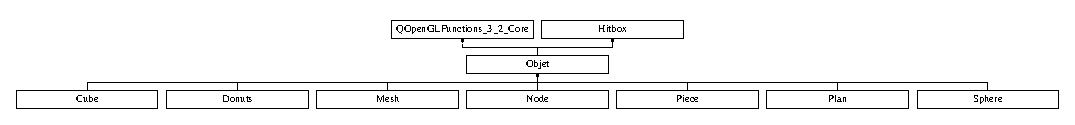
\includegraphics[height=1.230769cm]{class_objet}
\end{center}
\end{figure}
\subsection*{Public Member Functions}
\begin{DoxyCompactItemize}
\item 
\hyperlink{class_objet_aea29e90dc963beb399d3028b7322039f}{Objet} (const Q\+String \&\hyperlink{class_objet_a4a702c189bedcbf1e65da6aec72c8e44}{name}=Q\+String(), \hyperlink{class_material}{Material} $\ast$mat=N\+U\+L\+L, \hyperlink{structvec3}{vec3} \hyperlink{class_objet_ac69a1b459bcb4433099c8cfbff06b209}{rotation}=\hyperlink{structvec3}{vec3}(), \hyperlink{structvec3}{vec3} \hyperlink{class_objet_a0e109bc790b14328202dd2546b04e2fd}{position}=\hyperlink{structvec3}{vec3}(), \hyperlink{class_objet}{Objet} $\ast$\hyperlink{class_objet_a95e63a98dc9dc485fe874df30f2069ee}{parent}=N\+U\+L\+L)
\begin{DoxyCompactList}\small\item\em Constructeur. \end{DoxyCompactList}\item 
virtual \hyperlink{class_objet_a77a195bb1452ef4221b5080632cd7757}{$\sim$\+Objet} ()
\begin{DoxyCompactList}\small\item\em Destructeur. \end{DoxyCompactList}\item 
virtual void \hyperlink{class_objet_a5cc323f562964e00b947b2d908e206e7}{draw} ()
\begin{DoxyCompactList}\small\item\em Affichage de l'\hyperlink{class_objet}{Objet}. \end{DoxyCompactList}\item 
\hyperlink{structvec3}{vec3} \& \hyperlink{class_objet_a0e109bc790b14328202dd2546b04e2fd}{position} ()
\begin{DoxyCompactList}\small\item\em Récupère la position de l'\hyperlink{class_objet}{Objet}. \end{DoxyCompactList}\item 
\hyperlink{structvec3}{vec3} \hyperlink{class_objet_a79051e09eb1aa72dcd338ed033e9f3f1}{position} () const 
\begin{DoxyCompactList}\small\item\em Récupère la position de l'\hyperlink{class_objet}{Objet}. \end{DoxyCompactList}\item 
void \hyperlink{class_objet_a89ed090c598f087792ee81c40ff46f75}{position} (\hyperlink{structvec3}{vec3} p)
\begin{DoxyCompactList}\small\item\em Change la position de l'\hyperlink{class_objet}{Objet}. \end{DoxyCompactList}\item 
\hyperlink{structvec3}{vec3} \& \hyperlink{class_objet_ac69a1b459bcb4433099c8cfbff06b209}{rotation} ()
\begin{DoxyCompactList}\small\item\em Récupère la rotation de l'\hyperlink{class_objet}{Objet}. \end{DoxyCompactList}\item 
\hyperlink{structvec3}{vec3} \hyperlink{class_objet_a0325e52c600e8de17312287b4f7a3e67}{rotation} () const 
\begin{DoxyCompactList}\small\item\em Récupère la rotation de l'\hyperlink{class_objet}{Objet}. \end{DoxyCompactList}\item 
void \hyperlink{class_objet_a2d37f15368f40615a8bc58622623d991}{rotation} (\hyperlink{structvec3}{vec3} r)
\begin{DoxyCompactList}\small\item\em Change la rotation de l'\hyperlink{class_objet}{Objet}. \end{DoxyCompactList}\item 
void \hyperlink{class_objet_a13f08bf7d1265bbf4ade92b755b27c1b}{shader\+Id} (G\+Luint s)
\begin{DoxyCompactList}\small\item\em Change l'id du shader. \end{DoxyCompactList}\item 
\hyperlink{class_material}{Material} $\ast$ \hyperlink{class_objet_a5b8f371853435fb08bba5163cb4dbe09}{material} ()
\begin{DoxyCompactList}\small\item\em Récupère le material de l'\hyperlink{class_objet}{Objet}. \end{DoxyCompactList}\item 
void \hyperlink{class_objet_a470e028ee53141cf9d11d107317989b7}{material} (\hyperlink{class_material}{Material} $\ast$m)
\begin{DoxyCompactList}\small\item\em Change le \hyperlink{class_material}{Material} de l'\hyperlink{class_objet}{Objet}. \end{DoxyCompactList}\item 
void \hyperlink{class_objet_a95e63a98dc9dc485fe874df30f2069ee}{parent} (\hyperlink{class_objet}{Objet} $\ast$o)
\begin{DoxyCompactList}\small\item\em Change l'\hyperlink{class_objet}{Objet} père. \end{DoxyCompactList}\item 
\hyperlink{class_objet}{Objet} $\ast$ \hyperlink{class_objet_aaa3c3290e5bb742363263600fcdb3e5e}{parent} ()
\begin{DoxyCompactList}\small\item\em Récupère l'\hyperlink{class_objet}{Objet} père. \end{DoxyCompactList}\item 
const Q\+String \& \hyperlink{class_objet_a4a702c189bedcbf1e65da6aec72c8e44}{name} () const 
\begin{DoxyCompactList}\small\item\em Récupère le nom de l'\hyperlink{class_objet}{Objet}. \end{DoxyCompactList}\item 
void \hyperlink{class_objet_a9fcc9af481f4e13f46ab7d1b40cf91fc}{name} (const Q\+String \&n)
\begin{DoxyCompactList}\small\item\em Change le nom de l'\hyperlink{class_objet}{Objet}. \end{DoxyCompactList}\end{DoxyCompactItemize}
\subsection*{Protected Attributes}
\begin{DoxyCompactItemize}
\item 
\hyperlink{class_objet}{Objet} $\ast$ \hyperlink{class_objet_a91c5a50011c3fe9233a645aa767a275f}{\+\_\+parent}
\item 
\hyperlink{class_material}{Material} $\ast$ \hyperlink{class_objet_aefea82be8c63504190ac63d5e44ff61a}{\+\_\+mat}
\item 
Q\+String \hyperlink{class_objet_ac19f568a794dd9387386ee71914a868e}{\+\_\+name}
\item 
\hyperlink{structvec3}{vec3} \hyperlink{class_objet_a1d8675e88cc98ba740292af1421c2ee1}{\+\_\+rotation}
\item 
\hyperlink{structvec3}{vec3} \hyperlink{class_objet_a6c1a10fa5f4c5cd0e0617d93f42d927b}{\+\_\+position}
\item 
\hyperlink{structmat4}{mat4} \hyperlink{class_objet_a1963cca59f62c7a6f69a9c2c461ad9ea}{\+\_\+model}
\item 
G\+Luint \hyperlink{class_objet_af0d545a506dbfa377c8ca5a499fdf755}{\+\_\+shader\+Id}
\end{DoxyCompactItemize}
\subsection*{Private Member Functions}
\begin{DoxyCompactItemize}
\item 
void \hyperlink{class_objet_a0960722f5ddb16f2c245dca4e6584f25}{update\+Model} ()
\begin{DoxyCompactList}\small\item\em Met à jour la matrice de model. \end{DoxyCompactList}\item 
void \hyperlink{class_objet_a5c21e68142ae5b7c880cbd80336fb43e}{apply\+Material} ()
\begin{DoxyCompactList}\small\item\em Transmet les information du \hyperlink{class_material}{Material} au shader. \end{DoxyCompactList}\item 
void \hyperlink{class_objet_a995e953fb2f3d1a472aa04d2c5848f0a}{activate\+Shader} ()
\begin{DoxyCompactList}\small\item\em Change le shader actif. \end{DoxyCompactList}\end{DoxyCompactItemize}


\subsection{Detailed Description}
Classe de base affichable. 

\subsection{Constructor \& Destructor Documentation}
\hypertarget{class_objet_aea29e90dc963beb399d3028b7322039f}{\index{Objet@{Objet}!Objet@{Objet}}
\index{Objet@{Objet}!Objet@{Objet}}
\subsubsection[{Objet}]{\setlength{\rightskip}{0pt plus 5cm}Objet\+::\+Objet (
\begin{DoxyParamCaption}
\item[{const Q\+String \&}]{name = {\ttfamily QString()}, }
\item[{{\bf Material} $\ast$}]{mat = {\ttfamily NULL}, }
\item[{{\bf vec3}}]{rotation = {\ttfamily {\bf vec3}()}, }
\item[{{\bf vec3}}]{position = {\ttfamily {\bf vec3}()}, }
\item[{{\bf Objet} $\ast$}]{parent = {\ttfamily NULL}}
\end{DoxyParamCaption}
)}}\label{class_objet_aea29e90dc963beb399d3028b7322039f}


Constructeur. 

\hypertarget{class_objet_a77a195bb1452ef4221b5080632cd7757}{\index{Objet@{Objet}!````~Objet@{$\sim$\+Objet}}
\index{````~Objet@{$\sim$\+Objet}!Objet@{Objet}}
\subsubsection[{$\sim$\+Objet}]{\setlength{\rightskip}{0pt plus 5cm}virtual Objet\+::$\sim$\+Objet (
\begin{DoxyParamCaption}
{}
\end{DoxyParamCaption}
)\hspace{0.3cm}{\ttfamily [inline]}, {\ttfamily [virtual]}}}\label{class_objet_a77a195bb1452ef4221b5080632cd7757}


Destructeur. 



\subsection{Member Function Documentation}
\hypertarget{class_objet_a995e953fb2f3d1a472aa04d2c5848f0a}{\index{Objet@{Objet}!activate\+Shader@{activate\+Shader}}
\index{activate\+Shader@{activate\+Shader}!Objet@{Objet}}
\subsubsection[{activate\+Shader}]{\setlength{\rightskip}{0pt plus 5cm}void Objet\+::activate\+Shader (
\begin{DoxyParamCaption}
{}
\end{DoxyParamCaption}
)\hspace{0.3cm}{\ttfamily [private]}}}\label{class_objet_a995e953fb2f3d1a472aa04d2c5848f0a}


Change le shader actif. 

Active le shader de l'\hyperlink{class_objet}{Objet}, reporte les matrices de view et projection \hypertarget{class_objet_a5c21e68142ae5b7c880cbd80336fb43e}{\index{Objet@{Objet}!apply\+Material@{apply\+Material}}
\index{apply\+Material@{apply\+Material}!Objet@{Objet}}
\subsubsection[{apply\+Material}]{\setlength{\rightskip}{0pt plus 5cm}void Objet\+::apply\+Material (
\begin{DoxyParamCaption}
{}
\end{DoxyParamCaption}
)\hspace{0.3cm}{\ttfamily [private]}}}\label{class_objet_a5c21e68142ae5b7c880cbd80336fb43e}


Transmet les information du \hyperlink{class_material}{Material} au shader. 

Si l'\hyperlink{class_objet}{Objet} ne possède pas de \hyperlink{class_material}{Material} celui de son père est appliqué, s'il ne possède pas de père le dernier \hyperlink{class_material}{Material} est utilisé \hypertarget{class_objet_a5cc323f562964e00b947b2d908e206e7}{\index{Objet@{Objet}!draw@{draw}}
\index{draw@{draw}!Objet@{Objet}}
\subsubsection[{draw}]{\setlength{\rightskip}{0pt plus 5cm}void Objet\+::draw (
\begin{DoxyParamCaption}
{}
\end{DoxyParamCaption}
)\hspace{0.3cm}{\ttfamily [virtual]}}}\label{class_objet_a5cc323f562964e00b947b2d908e206e7}


Affichage de l'\hyperlink{class_objet}{Objet}. 

Active le shader de l'\hyperlink{class_objet}{Objet} et applique le material 

Reimplemented in \hyperlink{class_mesh_a996a8668fa2ca7d95d6d10744c833bc8}{Mesh}, \hyperlink{class_plan_a513c3dec0ce9043a9e1d3b5b18a6d698}{Plan}, \hyperlink{class_cube_ab26b72a81376fd5dc4fcc7f0b715b087}{Cube}, \hyperlink{class_piece_aee937e57fbfe4717aab14e1e892aed2e}{Piece}, \hyperlink{class_node_ab88c83ced58700a56de568f5b1e3c473}{Node}, \hyperlink{class_donuts_a5a7932c8494905ba09bb515a01e6c91d}{Donuts}, and \hyperlink{class_sphere_a34a34167b7544c95155d3ff30638d045}{Sphere}.

\hypertarget{class_objet_a5b8f371853435fb08bba5163cb4dbe09}{\index{Objet@{Objet}!material@{material}}
\index{material@{material}!Objet@{Objet}}
\subsubsection[{material}]{\setlength{\rightskip}{0pt plus 5cm}{\bf Material}$\ast$ Objet\+::material (
\begin{DoxyParamCaption}
{}
\end{DoxyParamCaption}
)\hspace{0.3cm}{\ttfamily [inline]}}}\label{class_objet_a5b8f371853435fb08bba5163cb4dbe09}


Récupère le material de l'\hyperlink{class_objet}{Objet}. 

\begin{DoxyReturn}{Returns}
un pointeur valide ou N\+U\+L\+L 
\end{DoxyReturn}
\hypertarget{class_objet_a470e028ee53141cf9d11d107317989b7}{\index{Objet@{Objet}!material@{material}}
\index{material@{material}!Objet@{Objet}}
\subsubsection[{material}]{\setlength{\rightskip}{0pt plus 5cm}void Objet\+::material (
\begin{DoxyParamCaption}
\item[{{\bf Material} $\ast$}]{m}
\end{DoxyParamCaption}
)\hspace{0.3cm}{\ttfamily [inline]}}}\label{class_objet_a470e028ee53141cf9d11d107317989b7}


Change le \hyperlink{class_material}{Material} de l'\hyperlink{class_objet}{Objet}. 


\begin{DoxyParams}{Parameters}
{\em m} & pointeur sur le nouveau \hyperlink{class_material}{Material} \\
\hline
\end{DoxyParams}
\hypertarget{class_objet_a4a702c189bedcbf1e65da6aec72c8e44}{\index{Objet@{Objet}!name@{name}}
\index{name@{name}!Objet@{Objet}}
\subsubsection[{name}]{\setlength{\rightskip}{0pt plus 5cm}const Q\+String\& Objet\+::name (
\begin{DoxyParamCaption}
{}
\end{DoxyParamCaption}
) const\hspace{0.3cm}{\ttfamily [inline]}}}\label{class_objet_a4a702c189bedcbf1e65da6aec72c8e44}


Récupère le nom de l'\hyperlink{class_objet}{Objet}. 

\begin{DoxyReturn}{Returns}
nom de l'\hyperlink{class_objet}{Objet} 
\end{DoxyReturn}
\hypertarget{class_objet_a9fcc9af481f4e13f46ab7d1b40cf91fc}{\index{Objet@{Objet}!name@{name}}
\index{name@{name}!Objet@{Objet}}
\subsubsection[{name}]{\setlength{\rightskip}{0pt plus 5cm}void Objet\+::name (
\begin{DoxyParamCaption}
\item[{const Q\+String \&}]{n}
\end{DoxyParamCaption}
)\hspace{0.3cm}{\ttfamily [inline]}}}\label{class_objet_a9fcc9af481f4e13f46ab7d1b40cf91fc}


Change le nom de l'\hyperlink{class_objet}{Objet}. 


\begin{DoxyParams}{Parameters}
{\em n} & nouveau nom de l'\hyperlink{class_objet}{Objet} \\
\hline
\end{DoxyParams}
\hypertarget{class_objet_a95e63a98dc9dc485fe874df30f2069ee}{\index{Objet@{Objet}!parent@{parent}}
\index{parent@{parent}!Objet@{Objet}}
\subsubsection[{parent}]{\setlength{\rightskip}{0pt plus 5cm}void Objet\+::parent (
\begin{DoxyParamCaption}
\item[{{\bf Objet} $\ast$}]{o}
\end{DoxyParamCaption}
)\hspace{0.3cm}{\ttfamily [inline]}}}\label{class_objet_a95e63a98dc9dc485fe874df30f2069ee}


Change l'\hyperlink{class_objet}{Objet} père. 


\begin{DoxyParams}{Parameters}
{\em o} & père \\
\hline
\end{DoxyParams}
\hypertarget{class_objet_aaa3c3290e5bb742363263600fcdb3e5e}{\index{Objet@{Objet}!parent@{parent}}
\index{parent@{parent}!Objet@{Objet}}
\subsubsection[{parent}]{\setlength{\rightskip}{0pt plus 5cm}{\bf Objet}$\ast$ Objet\+::parent (
\begin{DoxyParamCaption}
{}
\end{DoxyParamCaption}
)\hspace{0.3cm}{\ttfamily [inline]}}}\label{class_objet_aaa3c3290e5bb742363263600fcdb3e5e}


Récupère l'\hyperlink{class_objet}{Objet} père. 

\begin{DoxyReturn}{Returns}
\hyperlink{class_objet}{Objet} père ou N\+U\+L\+L 
\end{DoxyReturn}
\hypertarget{class_objet_a0e109bc790b14328202dd2546b04e2fd}{\index{Objet@{Objet}!position@{position}}
\index{position@{position}!Objet@{Objet}}
\subsubsection[{position}]{\setlength{\rightskip}{0pt plus 5cm}{\bf vec3}\& Objet\+::position (
\begin{DoxyParamCaption}
{}
\end{DoxyParamCaption}
)\hspace{0.3cm}{\ttfamily [inline]}}}\label{class_objet_a0e109bc790b14328202dd2546b04e2fd}


Récupère la position de l'\hyperlink{class_objet}{Objet}. 

\begin{DoxyReturn}{Returns}
position de l'\hyperlink{class_objet}{Objet} 
\end{DoxyReturn}
\hypertarget{class_objet_a79051e09eb1aa72dcd338ed033e9f3f1}{\index{Objet@{Objet}!position@{position}}
\index{position@{position}!Objet@{Objet}}
\subsubsection[{position}]{\setlength{\rightskip}{0pt plus 5cm}{\bf vec3} Objet\+::position (
\begin{DoxyParamCaption}
{}
\end{DoxyParamCaption}
) const\hspace{0.3cm}{\ttfamily [inline]}}}\label{class_objet_a79051e09eb1aa72dcd338ed033e9f3f1}


Récupère la position de l'\hyperlink{class_objet}{Objet}. 

\begin{DoxyReturn}{Returns}
position de l'\hyperlink{class_objet}{Objet} 
\end{DoxyReturn}
\hypertarget{class_objet_a89ed090c598f087792ee81c40ff46f75}{\index{Objet@{Objet}!position@{position}}
\index{position@{position}!Objet@{Objet}}
\subsubsection[{position}]{\setlength{\rightskip}{0pt plus 5cm}void Objet\+::position (
\begin{DoxyParamCaption}
\item[{{\bf vec3}}]{p}
\end{DoxyParamCaption}
)}}\label{class_objet_a89ed090c598f087792ee81c40ff46f75}


Change la position de l'\hyperlink{class_objet}{Objet}. 


\begin{DoxyParams}{Parameters}
{\em p} & nouvelle position \\
\hline
\end{DoxyParams}
\hypertarget{class_objet_ac69a1b459bcb4433099c8cfbff06b209}{\index{Objet@{Objet}!rotation@{rotation}}
\index{rotation@{rotation}!Objet@{Objet}}
\subsubsection[{rotation}]{\setlength{\rightskip}{0pt plus 5cm}{\bf vec3}\& Objet\+::rotation (
\begin{DoxyParamCaption}
{}
\end{DoxyParamCaption}
)\hspace{0.3cm}{\ttfamily [inline]}}}\label{class_objet_ac69a1b459bcb4433099c8cfbff06b209}


Récupère la rotation de l'\hyperlink{class_objet}{Objet}. 

\begin{DoxyReturn}{Returns}
rotation de l'\hyperlink{class_objet}{Objet} 
\end{DoxyReturn}
\hypertarget{class_objet_a0325e52c600e8de17312287b4f7a3e67}{\index{Objet@{Objet}!rotation@{rotation}}
\index{rotation@{rotation}!Objet@{Objet}}
\subsubsection[{rotation}]{\setlength{\rightskip}{0pt plus 5cm}{\bf vec3} Objet\+::rotation (
\begin{DoxyParamCaption}
{}
\end{DoxyParamCaption}
) const\hspace{0.3cm}{\ttfamily [inline]}}}\label{class_objet_a0325e52c600e8de17312287b4f7a3e67}


Récupère la rotation de l'\hyperlink{class_objet}{Objet}. 

\begin{DoxyReturn}{Returns}
rotation de l'\hyperlink{class_objet}{Objet} 
\end{DoxyReturn}
\hypertarget{class_objet_a2d37f15368f40615a8bc58622623d991}{\index{Objet@{Objet}!rotation@{rotation}}
\index{rotation@{rotation}!Objet@{Objet}}
\subsubsection[{rotation}]{\setlength{\rightskip}{0pt plus 5cm}void Objet\+::rotation (
\begin{DoxyParamCaption}
\item[{{\bf vec3}}]{r}
\end{DoxyParamCaption}
)}}\label{class_objet_a2d37f15368f40615a8bc58622623d991}


Change la rotation de l'\hyperlink{class_objet}{Objet}. 


\begin{DoxyParams}{Parameters}
{\em r} & nouvelle rotation de l'\hyperlink{class_objet}{Objet} \\
\hline
\end{DoxyParams}
\hypertarget{class_objet_a13f08bf7d1265bbf4ade92b755b27c1b}{\index{Objet@{Objet}!shader\+Id@{shader\+Id}}
\index{shader\+Id@{shader\+Id}!Objet@{Objet}}
\subsubsection[{shader\+Id}]{\setlength{\rightskip}{0pt plus 5cm}void Objet\+::shader\+Id (
\begin{DoxyParamCaption}
\item[{G\+Luint}]{s}
\end{DoxyParamCaption}
)\hspace{0.3cm}{\ttfamily [inline]}}}\label{class_objet_a13f08bf7d1265bbf4ade92b755b27c1b}


Change l'id du shader. 


\begin{DoxyParams}{Parameters}
{\em s} & nouvel id du shader de l'\hyperlink{class_objet}{Objet} \\
\hline
\end{DoxyParams}
\hypertarget{class_objet_a0960722f5ddb16f2c245dca4e6584f25}{\index{Objet@{Objet}!update\+Model@{update\+Model}}
\index{update\+Model@{update\+Model}!Objet@{Objet}}
\subsubsection[{update\+Model}]{\setlength{\rightskip}{0pt plus 5cm}void Objet\+::update\+Model (
\begin{DoxyParamCaption}
{}
\end{DoxyParamCaption}
)\hspace{0.3cm}{\ttfamily [private]}}}\label{class_objet_a0960722f5ddb16f2c245dca4e6584f25}


Met à jour la matrice de model. 

Appellée lors d'une modification des vecteurs position ou rotation 

\subsection{Member Data Documentation}
\hypertarget{class_objet_aefea82be8c63504190ac63d5e44ff61a}{\index{Objet@{Objet}!\+\_\+mat@{\+\_\+mat}}
\index{\+\_\+mat@{\+\_\+mat}!Objet@{Objet}}
\subsubsection[{\+\_\+mat}]{\setlength{\rightskip}{0pt plus 5cm}{\bf Material}$\ast$ Objet\+::\+\_\+mat\hspace{0.3cm}{\ttfamily [protected]}}}\label{class_objet_aefea82be8c63504190ac63d5e44ff61a}
\hypertarget{class_objet_a1963cca59f62c7a6f69a9c2c461ad9ea}{\index{Objet@{Objet}!\+\_\+model@{\+\_\+model}}
\index{\+\_\+model@{\+\_\+model}!Objet@{Objet}}
\subsubsection[{\+\_\+model}]{\setlength{\rightskip}{0pt plus 5cm}{\bf mat4} Objet\+::\+\_\+model\hspace{0.3cm}{\ttfamily [protected]}}}\label{class_objet_a1963cca59f62c7a6f69a9c2c461ad9ea}
\hypertarget{class_objet_ac19f568a794dd9387386ee71914a868e}{\index{Objet@{Objet}!\+\_\+name@{\+\_\+name}}
\index{\+\_\+name@{\+\_\+name}!Objet@{Objet}}
\subsubsection[{\+\_\+name}]{\setlength{\rightskip}{0pt plus 5cm}Q\+String Objet\+::\+\_\+name\hspace{0.3cm}{\ttfamily [protected]}}}\label{class_objet_ac19f568a794dd9387386ee71914a868e}
\hypertarget{class_objet_a91c5a50011c3fe9233a645aa767a275f}{\index{Objet@{Objet}!\+\_\+parent@{\+\_\+parent}}
\index{\+\_\+parent@{\+\_\+parent}!Objet@{Objet}}
\subsubsection[{\+\_\+parent}]{\setlength{\rightskip}{0pt plus 5cm}{\bf Objet}$\ast$ Objet\+::\+\_\+parent\hspace{0.3cm}{\ttfamily [protected]}}}\label{class_objet_a91c5a50011c3fe9233a645aa767a275f}
\hypertarget{class_objet_a6c1a10fa5f4c5cd0e0617d93f42d927b}{\index{Objet@{Objet}!\+\_\+position@{\+\_\+position}}
\index{\+\_\+position@{\+\_\+position}!Objet@{Objet}}
\subsubsection[{\+\_\+position}]{\setlength{\rightskip}{0pt plus 5cm}{\bf vec3} Objet\+::\+\_\+position\hspace{0.3cm}{\ttfamily [protected]}}}\label{class_objet_a6c1a10fa5f4c5cd0e0617d93f42d927b}
\hypertarget{class_objet_a1d8675e88cc98ba740292af1421c2ee1}{\index{Objet@{Objet}!\+\_\+rotation@{\+\_\+rotation}}
\index{\+\_\+rotation@{\+\_\+rotation}!Objet@{Objet}}
\subsubsection[{\+\_\+rotation}]{\setlength{\rightskip}{0pt plus 5cm}{\bf vec3} Objet\+::\+\_\+rotation\hspace{0.3cm}{\ttfamily [protected]}}}\label{class_objet_a1d8675e88cc98ba740292af1421c2ee1}
\hypertarget{class_objet_af0d545a506dbfa377c8ca5a499fdf755}{\index{Objet@{Objet}!\+\_\+shader\+Id@{\+\_\+shader\+Id}}
\index{\+\_\+shader\+Id@{\+\_\+shader\+Id}!Objet@{Objet}}
\subsubsection[{\+\_\+shader\+Id}]{\setlength{\rightskip}{0pt plus 5cm}G\+Luint Objet\+::\+\_\+shader\+Id\hspace{0.3cm}{\ttfamily [protected]}}}\label{class_objet_af0d545a506dbfa377c8ca5a499fdf755}


The documentation for this class was generated from the following files\+:\begin{DoxyCompactItemize}
\item 
objets/\hyperlink{objet_8hpp}{objet.\+hpp}\item 
objets/\hyperlink{objet_8cpp}{objet.\+cpp}\end{DoxyCompactItemize}

\hypertarget{class_piece}{\section{Référence de la classe Piece}
\label{class_piece}\index{Piece@{Piece}}
}


Pièce, contient un ensemble d'objet qu'elle contient.  




{\ttfamily \#include $<$piece.\+hpp$>$}



Graphe d'héritage de Piece\+:
\nopagebreak
\begin{figure}[H]
\begin{center}
\leavevmode
\includegraphics[height=550pt]{class_piece__inherit__graph}
\end{center}
\end{figure}


Graphe de collaboration de Piece\+:
\nopagebreak
\begin{figure}[H]
\begin{center}
\leavevmode
\includegraphics[height=550pt]{class_piece__coll__graph}
\end{center}
\end{figure}
\subsection*{Fonctions membres publiques}
\begin{DoxyCompactItemize}
\item 
\hyperlink{class_piece_adfc1a07bd6a58ab6cac476fedb38cb15}{Piece} (\hyperlink{structvec3}{vec3} dimension=\hyperlink{structvec3}{vec3}(1, 1, 1), \hyperlink{structvec3}{vec3} \hyperlink{class_objet_ac69a1b459bcb4433099c8cfbff06b209}{rotation}=\hyperlink{structvec3}{vec3}(), \hyperlink{structvec3}{vec3} \hyperlink{class_objet_a0e109bc790b14328202dd2546b04e2fd}{position}=\hyperlink{structvec3}{vec3}(), \hyperlink{class_material}{Material} $\ast$mat=N\+U\+L\+L)
\begin{DoxyCompactList}\small\item\em Constructeur. \end{DoxyCompactList}\item 
\hyperlink{class_piece_a5d7a4f6bade94cb33b6f634de8aa7918}{$\sim$\+Piece} ()
\begin{DoxyCompactList}\small\item\em Destructeur. \end{DoxyCompactList}\item 
void \hyperlink{class_piece_aee937e57fbfe4717aab14e1e892aed2e}{draw} ()
\begin{DoxyCompactList}\small\item\em Affiche l'ensemble des fils. \end{DoxyCompactList}\item 
void \hyperlink{class_piece_adf4f51a5f33071fd0acc706c347f4741}{add\+Child} (const Q\+String \&\hyperlink{class_objet_a4a702c189bedcbf1e65da6aec72c8e44}{name}, \hyperlink{class_objet}{Objet} $\ast$objet)
\begin{DoxyCompactList}\small\item\em Ajoute un fils à la pièce. \end{DoxyCompactList}\item 
void \hyperlink{class_piece_aeb48b4fda2f8950546baf534b3cf08cf}{add\+Child} (\hyperlink{class_objet}{Objet} $\ast$o)
\begin{DoxyCompactList}\small\item\em Ajoute un fils à la pièce. \end{DoxyCompactList}\item 
Q\+String\+List \hyperlink{class_piece_a029823aa5135b356a9e4da14578db4e8}{get\+Children} () const 
\begin{DoxyCompactList}\small\item\em Récupère la liste des noms des objets fils. \end{DoxyCompactList}\item 
\hyperlink{class_objet}{Objet} $\ast$ \hyperlink{class_piece_aa77dc9ed8493cc22d1455c3eb2bec013}{get\+Child} (const Q\+String \&\hyperlink{class_objet_a4a702c189bedcbf1e65da6aec72c8e44}{name})
\begin{DoxyCompactList}\small\item\em Renvoie un pointeur sur un objet fils. \end{DoxyCompactList}\item 
void \hyperlink{class_piece_a133ad0c10c91b183fb145fe54ea6c0f1}{remove\+Child} (const Q\+String \&\hyperlink{class_objet_a4a702c189bedcbf1e65da6aec72c8e44}{name})
\begin{DoxyCompactList}\small\item\em enlève un \hyperlink{class_objet}{Objet} fils de la pièce \end{DoxyCompactList}\item 
void \hyperlink{class_piece_a49b725ce33449c3099253288ea261349}{delete\+Child} (const Q\+String \&\hyperlink{class_objet_a4a702c189bedcbf1e65da6aec72c8e44}{name})
\begin{DoxyCompactList}\small\item\em supprime un \hyperlink{class_objet}{Objet} fils de la \hyperlink{class_piece}{Piece} \end{DoxyCompactList}\item 
const \hyperlink{structvec3}{vec3} \& \hyperlink{class_piece_afbfee8c5de17e5b046bcddd83043e5b6}{dimensions} () const 
\begin{DoxyCompactList}\small\item\em Retourne les dimensions de la pièce. \end{DoxyCompactList}\item 
\hyperlink{structvec3}{vec3} \& \hyperlink{class_piece_a3f5440ec22866d79a26a513470744412}{dimensions} ()
\begin{DoxyCompactList}\small\item\em Retourne les dimensions de la pièce. \end{DoxyCompactList}\item 
void \hyperlink{class_piece_a4419c3b0a9e57dcd215dd87be025752f}{dimensions} (const \hyperlink{structvec3}{vec3} v)
\begin{DoxyCompactList}\small\item\em Edite les dimensions de la pièce. \end{DoxyCompactList}\end{DoxyCompactItemize}
\subsection*{Attributs privés}
\begin{DoxyCompactItemize}
\item 
\hyperlink{structvec3}{vec3} \hyperlink{class_piece_a47a3458694b894041bd95a1666c9bf3d}{\+\_\+dimensions}
\item 
Q\+Map$<$ Q\+String, \hyperlink{class_objet}{Objet} $\ast$ $>$ \hyperlink{class_piece_ac80078a597e7edcd297895bab25731e6}{\+\_\+children}
\end{DoxyCompactItemize}
\subsection*{Membres hérités additionnels}


\subsection{Description détaillée}
Pièce, contient un ensemble d'objet qu'elle contient. 

\subsection{Documentation des constructeurs et destructeur}
\hypertarget{class_piece_adfc1a07bd6a58ab6cac476fedb38cb15}{\index{Piece@{Piece}!Piece@{Piece}}
\index{Piece@{Piece}!Piece@{Piece}}
\subsubsection[{Piece}]{\setlength{\rightskip}{0pt plus 5cm}Piece\+::\+Piece (
\begin{DoxyParamCaption}
\item[{{\bf vec3}}]{dimension = {\ttfamily {\bf vec3}(1,1,1)}, }
\item[{{\bf vec3}}]{rotation = {\ttfamily {\bf vec3}()}, }
\item[{{\bf vec3}}]{position = {\ttfamily {\bf vec3}()}, }
\item[{{\bf Material} $\ast$}]{mat = {\ttfamily NULL}}
\end{DoxyParamCaption}
)}}\label{class_piece_adfc1a07bd6a58ab6cac476fedb38cb15}


Constructeur. 

Liste des objets fils de la pièces, contient au moins les murs \hypertarget{class_piece_a5d7a4f6bade94cb33b6f634de8aa7918}{\index{Piece@{Piece}!````~Piece@{$\sim$\+Piece}}
\index{````~Piece@{$\sim$\+Piece}!Piece@{Piece}}
\subsubsection[{$\sim$\+Piece}]{\setlength{\rightskip}{0pt plus 5cm}Piece\+::$\sim$\+Piece (
\begin{DoxyParamCaption}
{}
\end{DoxyParamCaption}
)}}\label{class_piece_a5d7a4f6bade94cb33b6f634de8aa7918}


Destructeur. 



\subsection{Documentation des fonctions membres}
\hypertarget{class_piece_adf4f51a5f33071fd0acc706c347f4741}{\index{Piece@{Piece}!add\+Child@{add\+Child}}
\index{add\+Child@{add\+Child}!Piece@{Piece}}
\subsubsection[{add\+Child}]{\setlength{\rightskip}{0pt plus 5cm}void Piece\+::add\+Child (
\begin{DoxyParamCaption}
\item[{const Q\+String \&}]{name, }
\item[{{\bf Objet} $\ast$}]{objet}
\end{DoxyParamCaption}
)}}\label{class_piece_adf4f51a5f33071fd0acc706c347f4741}


Ajoute un fils à la pièce. 

Se charge de la destruction de l'objet


\begin{DoxyParams}{Paramètres}
{\em name} & nom de l'objet \\
\hline
{\em objet} & objet à ajouter \\
\hline
\end{DoxyParams}


Voici le graphe d'appel pour cette fonction \+:
\nopagebreak
\begin{figure}[H]
\begin{center}
\leavevmode
\includegraphics[width=273pt]{class_piece_adf4f51a5f33071fd0acc706c347f4741_cgraph}
\end{center}
\end{figure}


\hypertarget{class_piece_aeb48b4fda2f8950546baf534b3cf08cf}{\index{Piece@{Piece}!add\+Child@{add\+Child}}
\index{add\+Child@{add\+Child}!Piece@{Piece}}
\subsubsection[{add\+Child}]{\setlength{\rightskip}{0pt plus 5cm}void Piece\+::add\+Child (
\begin{DoxyParamCaption}
\item[{{\bf Objet} $\ast$}]{o}
\end{DoxyParamCaption}
)}}\label{class_piece_aeb48b4fda2f8950546baf534b3cf08cf}


Ajoute un fils à la pièce. 


\begin{DoxyParams}{Paramètres}
{\em o} & objet à ajouter \\
\hline
\end{DoxyParams}


Voici le graphe d'appel pour cette fonction \+:
\nopagebreak
\begin{figure}[H]
\begin{center}
\leavevmode
\includegraphics[width=273pt]{class_piece_aeb48b4fda2f8950546baf534b3cf08cf_cgraph}
\end{center}
\end{figure}


\hypertarget{class_piece_a49b725ce33449c3099253288ea261349}{\index{Piece@{Piece}!delete\+Child@{delete\+Child}}
\index{delete\+Child@{delete\+Child}!Piece@{Piece}}
\subsubsection[{delete\+Child}]{\setlength{\rightskip}{0pt plus 5cm}void Piece\+::delete\+Child (
\begin{DoxyParamCaption}
\item[{const Q\+String \&}]{name}
\end{DoxyParamCaption}
)}}\label{class_piece_a49b725ce33449c3099253288ea261349}


supprime un \hyperlink{class_objet}{Objet} fils de la \hyperlink{class_piece}{Piece} 

supprime l'\hyperlink{class_objet}{Objet} et libère la mémoire associé


\begin{DoxyParams}{Paramètres}
{\em name} & nom de l'\hyperlink{class_objet}{Objet} \\
\hline
\end{DoxyParams}
\hypertarget{class_piece_afbfee8c5de17e5b046bcddd83043e5b6}{\index{Piece@{Piece}!dimensions@{dimensions}}
\index{dimensions@{dimensions}!Piece@{Piece}}
\subsubsection[{dimensions}]{\setlength{\rightskip}{0pt plus 5cm}const {\bf vec3} \& Piece\+::dimensions (
\begin{DoxyParamCaption}
{}
\end{DoxyParamCaption}
) const}}\label{class_piece_afbfee8c5de17e5b046bcddd83043e5b6}


Retourne les dimensions de la pièce. 

\begin{DoxyReturn}{Renvoie}
\hyperlink{structvec3}{vec3} contenant les dimensions de la pièce 
\end{DoxyReturn}
\hypertarget{class_piece_a3f5440ec22866d79a26a513470744412}{\index{Piece@{Piece}!dimensions@{dimensions}}
\index{dimensions@{dimensions}!Piece@{Piece}}
\subsubsection[{dimensions}]{\setlength{\rightskip}{0pt plus 5cm}{\bf vec3} \& Piece\+::dimensions (
\begin{DoxyParamCaption}
{}
\end{DoxyParamCaption}
)}}\label{class_piece_a3f5440ec22866d79a26a513470744412}


Retourne les dimensions de la pièce. 

\begin{DoxyReturn}{Renvoie}
\hyperlink{structvec3}{vec3} contenant les dimensions de la pièce 
\end{DoxyReturn}
\hypertarget{class_piece_a4419c3b0a9e57dcd215dd87be025752f}{\index{Piece@{Piece}!dimensions@{dimensions}}
\index{dimensions@{dimensions}!Piece@{Piece}}
\subsubsection[{dimensions}]{\setlength{\rightskip}{0pt plus 5cm}void Piece\+::dimensions (
\begin{DoxyParamCaption}
\item[{const {\bf vec3}}]{v}
\end{DoxyParamCaption}
)}}\label{class_piece_a4419c3b0a9e57dcd215dd87be025752f}


Edite les dimensions de la pièce. 


\begin{DoxyParams}{Paramètres}
{\em v} & nouvelles dimensions de la pièce \\
\hline
\end{DoxyParams}
\hypertarget{class_piece_aee937e57fbfe4717aab14e1e892aed2e}{\index{Piece@{Piece}!draw@{draw}}
\index{draw@{draw}!Piece@{Piece}}
\subsubsection[{draw}]{\setlength{\rightskip}{0pt plus 5cm}void Piece\+::draw (
\begin{DoxyParamCaption}
{}
\end{DoxyParamCaption}
)\hspace{0.3cm}{\ttfamily [virtual]}}}\label{class_piece_aee937e57fbfe4717aab14e1e892aed2e}


Affiche l'ensemble des fils. 



Réimplémentée à partir de \hyperlink{class_objet_a5cc323f562964e00b947b2d908e206e7}{Objet}.



Voici le graphe d'appel pour cette fonction \+:
\nopagebreak
\begin{figure}[H]
\begin{center}
\leavevmode
\includegraphics[width=259pt]{class_piece_aee937e57fbfe4717aab14e1e892aed2e_cgraph}
\end{center}
\end{figure}


\hypertarget{class_piece_aa77dc9ed8493cc22d1455c3eb2bec013}{\index{Piece@{Piece}!get\+Child@{get\+Child}}
\index{get\+Child@{get\+Child}!Piece@{Piece}}
\subsubsection[{get\+Child}]{\setlength{\rightskip}{0pt plus 5cm}{\bf Objet} $\ast$ Piece\+::get\+Child (
\begin{DoxyParamCaption}
\item[{const Q\+String \&}]{name}
\end{DoxyParamCaption}
)}}\label{class_piece_aa77dc9ed8493cc22d1455c3eb2bec013}


Renvoie un pointeur sur un objet fils. 

Récupère un pointeur sur un objet fils de la pièce


\begin{DoxyParams}{Paramètres}
{\em name} & nom de l'objet \\
\hline
\end{DoxyParams}
\begin{DoxyReturn}{Renvoie}
un pointeur valide si l'objet est un fils de la pièce, N\+U\+L\+L sinon 
\end{DoxyReturn}


Voici le graphe des appelants de cette fonction \+:
\nopagebreak
\begin{figure}[H]
\begin{center}
\leavevmode
\includegraphics[width=350pt]{class_piece_aa77dc9ed8493cc22d1455c3eb2bec013_icgraph}
\end{center}
\end{figure}


\hypertarget{class_piece_a029823aa5135b356a9e4da14578db4e8}{\index{Piece@{Piece}!get\+Children@{get\+Children}}
\index{get\+Children@{get\+Children}!Piece@{Piece}}
\subsubsection[{get\+Children}]{\setlength{\rightskip}{0pt plus 5cm}Q\+String\+List Piece\+::get\+Children (
\begin{DoxyParamCaption}
{}
\end{DoxyParamCaption}
) const}}\label{class_piece_a029823aa5135b356a9e4da14578db4e8}


Récupère la liste des noms des objets fils. 

\begin{DoxyRefDesc}{A faire}
\item[\hyperlink{todo__todo000004}{A faire}]A revoir ! \begin{DoxyReturn}{Renvoie}
liste des noms des objets 
\end{DoxyReturn}
\end{DoxyRefDesc}


Voici le graphe des appelants de cette fonction \+:
\nopagebreak
\begin{figure}[H]
\begin{center}
\leavevmode
\includegraphics[width=350pt]{class_piece_a029823aa5135b356a9e4da14578db4e8_icgraph}
\end{center}
\end{figure}


\hypertarget{class_piece_a133ad0c10c91b183fb145fe54ea6c0f1}{\index{Piece@{Piece}!remove\+Child@{remove\+Child}}
\index{remove\+Child@{remove\+Child}!Piece@{Piece}}
\subsubsection[{remove\+Child}]{\setlength{\rightskip}{0pt plus 5cm}void Piece\+::remove\+Child (
\begin{DoxyParamCaption}
\item[{const Q\+String \&}]{name}
\end{DoxyParamCaption}
)}}\label{class_piece_a133ad0c10c91b183fb145fe54ea6c0f1}


enlève un \hyperlink{class_objet}{Objet} fils de la pièce 


\begin{DoxyParams}{Paramètres}
{\em name} & nom de l'\hyperlink{class_objet}{Objet} à supprimer \\
\hline
\end{DoxyParams}


\subsection{Documentation des données membres}
\hypertarget{class_piece_ac80078a597e7edcd297895bab25731e6}{\index{Piece@{Piece}!\+\_\+children@{\+\_\+children}}
\index{\+\_\+children@{\+\_\+children}!Piece@{Piece}}
\subsubsection[{\+\_\+children}]{\setlength{\rightskip}{0pt plus 5cm}Q\+Map$<$Q\+String, {\bf Objet} $\ast$$>$ Piece\+::\+\_\+children\hspace{0.3cm}{\ttfamily [private]}}}\label{class_piece_ac80078a597e7edcd297895bab25731e6}
\hypertarget{class_piece_a47a3458694b894041bd95a1666c9bf3d}{\index{Piece@{Piece}!\+\_\+dimensions@{\+\_\+dimensions}}
\index{\+\_\+dimensions@{\+\_\+dimensions}!Piece@{Piece}}
\subsubsection[{\+\_\+dimensions}]{\setlength{\rightskip}{0pt plus 5cm}{\bf vec3} Piece\+::\+\_\+dimensions\hspace{0.3cm}{\ttfamily [private]}}}\label{class_piece_a47a3458694b894041bd95a1666c9bf3d}
Contient les dimensions de la pièces 

La documentation de cette classe a été générée à partir des fichiers suivants \+:\begin{DoxyCompactItemize}
\item 
scene/\hyperlink{piece_8hpp}{piece.\+hpp}\item 
scene/\hyperlink{piece_8cpp}{piece.\+cpp}\end{DoxyCompactItemize}

\hypertarget{class_plan}{\section{Plan Class Reference}
\label{class_plan}\index{Plan@{Plan}}
}


\hyperlink{class_plan}{Plan} utilisé par la \hyperlink{class_piece}{Piece}.  




{\ttfamily \#include $<$plan.\+hpp$>$}

Inheritance diagram for Plan\+:\begin{figure}[H]
\begin{center}
\leavevmode
\includegraphics[height=3.000000cm]{class_plan}
\end{center}
\end{figure}
\subsection*{Public Member Functions}
\begin{DoxyCompactItemize}
\item 
\hyperlink{class_plan_ab74eeb948e40ade24bd54a60a4ece8c6}{Plan} (int width=1, int height=1, int width\+Division=1, int height\+Division=1, const Q\+List$<$ Q\+Rect\+F $>$ rects=Q\+List$<$ Q\+Rect\+F $>$(), \hyperlink{class_material}{Material} $\ast$mat=N\+U\+L\+L, \hyperlink{structvec3}{vec3} \hyperlink{class_objet_ac69a1b459bcb4433099c8cfbff06b209}{rotation}=\hyperlink{structvec3}{vec3}(), \hyperlink{structvec3}{vec3} \hyperlink{class_objet_a0e109bc790b14328202dd2546b04e2fd}{position}=\hyperlink{structvec3}{vec3}())
\begin{DoxyCompactList}\small\item\em Constructeur. \end{DoxyCompactList}\item 
\hyperlink{class_plan_a4df05d0211ed4572125f79cbfaafa626}{$\sim$\+Plan} ()
\begin{DoxyCompactList}\small\item\em Destructeur. \end{DoxyCompactList}\item 
void \hyperlink{class_plan_a513c3dec0ce9043a9e1d3b5b18a6d698}{draw} ()
\begin{DoxyCompactList}\small\item\em Affiche le plan. \end{DoxyCompactList}\item 
const Q\+List$<$ Q\+Rect\+F $>$ \& \hyperlink{class_plan_ac193f6297c584d43977dca3a16f18180}{get\+Fenetres} () const 
\begin{DoxyCompactList}\small\item\em Renvoie la liste des rectangles définissant les fenêtres de la pièce. \end{DoxyCompactList}\end{DoxyCompactItemize}
\subsection*{Protected Member Functions}
\begin{DoxyCompactItemize}
\item 
virtual \hyperlink{structvec3}{vec3} \hyperlink{class_plan_a2561b08d2e0f333c56d7ac2b5cc72fd7}{get\+P} () const 
\item 
virtual float \hyperlink{class_plan_aa64cc1ec4e6d1660c691592eb441e00c}{get\+Width} () const 
\item 
virtual float \hyperlink{class_plan_a73316993ed03bbf13b38f2dff76b0ced}{get\+Height} () const 
\item 
virtual float \hyperlink{class_plan_a086041dcf2879904e774f34ae4ad61d7}{get\+Depth} () const 
\end{DoxyCompactItemize}
\subsection*{Private Attributes}
\begin{DoxyCompactItemize}
\item 
G\+Luint \hyperlink{class_plan_ab4efe8532b73dd0efca80000afb0027d}{\+\_\+vao}
\item 
G\+Luint \hyperlink{class_plan_a7b203dc36964da663836cf7614fe711a}{\+\_\+vbo\+\_\+vertices}
\item 
G\+Luint \hyperlink{class_plan_aa5db33661be2dfcecf68683c33eb22b9}{\+\_\+vbo\+\_\+normals}
\item 
G\+Luint \hyperlink{class_plan_ad8791ad67d66ac1b24792dc72ec00c64}{\+\_\+vbo\+\_\+indices}
\item 
G\+Luint \hyperlink{class_plan_a3c16becd29f35260b79af8b9cb6fa892}{\+\_\+vbo\+\_\+tex\+Coord}
\item 
unsigned int \hyperlink{class_plan_af3d9228c1b7dc91c0cb00d4c8fa5a550}{\+\_\+nb\+Vertices}
\item 
\hyperlink{structvec3}{vec3} \hyperlink{class_plan_aad9837a269e87fa5d7a4a5fc90abf3e7}{\+\_\+min\+P}
\item 
\hyperlink{structvec3}{vec3} \hyperlink{class_plan_a2dce54e58d00f40ed8da5c9bd34c1232}{\+\_\+max\+P}
\item 
Q\+List$<$ Q\+Rect\+F $>$ \hyperlink{class_plan_aa9fdbf8efac3f80ffd8bb2f789e7f4f2}{\+\_\+fenetres}
\end{DoxyCompactItemize}
\subsection*{Additional Inherited Members}


\subsection{Detailed Description}
\hyperlink{class_plan}{Plan} utilisé par la \hyperlink{class_piece}{Piece}. 

Gère un plan, avec des trous pour les fenêtres 

\subsection{Constructor \& Destructor Documentation}
\hypertarget{class_plan_ab74eeb948e40ade24bd54a60a4ece8c6}{\index{Plan@{Plan}!Plan@{Plan}}
\index{Plan@{Plan}!Plan@{Plan}}
\subsubsection[{Plan}]{\setlength{\rightskip}{0pt plus 5cm}Plan\+::\+Plan (
\begin{DoxyParamCaption}
\item[{int}]{width = {\ttfamily 1}, }
\item[{int}]{height = {\ttfamily 1}, }
\item[{int}]{width\+Division = {\ttfamily 1}, }
\item[{int}]{height\+Division = {\ttfamily 1}, }
\item[{const Q\+List$<$ Q\+Rect\+F $>$}]{rects = {\ttfamily QList$<$QRectF$>$()}, }
\item[{{\bf Material} $\ast$}]{mat = {\ttfamily NULL}, }
\item[{{\bf vec3}}]{rotation = {\ttfamily {\bf vec3}()}, }
\item[{{\bf vec3}}]{position = {\ttfamily {\bf vec3}()}}
\end{DoxyParamCaption}
)}}\label{class_plan_ab74eeb948e40ade24bd54a60a4ece8c6}


Constructeur. 


\begin{DoxyParams}{Parameters}
{\em width} & largeur du plan \\
\hline
{\em height} & hauteur du plan \\
\hline
{\em width\+Division} & nombre de division selon width \\
\hline
{\em height\+Division} & nombre de division selon height \\
\hline
{\em rects} & Q\+Rect\+F rectangles définissant les fenêtres du plan \\
\hline
{\em mat} & \hyperlink{class_material}{Material} à utiliser \\
\hline
{\em rotation} & rotation à appliquer au plan \\
\hline
{\em position} & position du plan dans le monde \\
\hline
\end{DoxyParams}
\hypertarget{class_plan_a4df05d0211ed4572125f79cbfaafa626}{\index{Plan@{Plan}!````~Plan@{$\sim$\+Plan}}
\index{````~Plan@{$\sim$\+Plan}!Plan@{Plan}}
\subsubsection[{$\sim$\+Plan}]{\setlength{\rightskip}{0pt plus 5cm}Plan\+::$\sim$\+Plan (
\begin{DoxyParamCaption}
{}
\end{DoxyParamCaption}
)}}\label{class_plan_a4df05d0211ed4572125f79cbfaafa626}


Destructeur. 

Détruit le plan et libère les vbo/vba 

\subsection{Member Function Documentation}
\hypertarget{class_plan_a513c3dec0ce9043a9e1d3b5b18a6d698}{\index{Plan@{Plan}!draw@{draw}}
\index{draw@{draw}!Plan@{Plan}}
\subsubsection[{draw}]{\setlength{\rightskip}{0pt plus 5cm}void Plan\+::draw (
\begin{DoxyParamCaption}
{}
\end{DoxyParamCaption}
)\hspace{0.3cm}{\ttfamily [virtual]}}}\label{class_plan_a513c3dec0ce9043a9e1d3b5b18a6d698}


Affiche le plan. 



Reimplemented from \hyperlink{class_objet_a5cc323f562964e00b947b2d908e206e7}{Objet}.

\hypertarget{class_plan_a086041dcf2879904e774f34ae4ad61d7}{\index{Plan@{Plan}!get\+Depth@{get\+Depth}}
\index{get\+Depth@{get\+Depth}!Plan@{Plan}}
\subsubsection[{get\+Depth}]{\setlength{\rightskip}{0pt plus 5cm}float Plan\+::get\+Depth (
\begin{DoxyParamCaption}
{}
\end{DoxyParamCaption}
) const\hspace{0.3cm}{\ttfamily [protected]}, {\ttfamily [virtual]}}}\label{class_plan_a086041dcf2879904e774f34ae4ad61d7}
\hypertarget{class_plan_ac193f6297c584d43977dca3a16f18180}{\index{Plan@{Plan}!get\+Fenetres@{get\+Fenetres}}
\index{get\+Fenetres@{get\+Fenetres}!Plan@{Plan}}
\subsubsection[{get\+Fenetres}]{\setlength{\rightskip}{0pt plus 5cm}const Q\+List$<$Q\+Rect\+F$>$\& Plan\+::get\+Fenetres (
\begin{DoxyParamCaption}
{}
\end{DoxyParamCaption}
) const\hspace{0.3cm}{\ttfamily [inline]}}}\label{class_plan_ac193f6297c584d43977dca3a16f18180}


Renvoie la liste des rectangles définissant les fenêtres de la pièce. 

\begin{DoxyReturn}{Returns}
liste des fenêtres 
\end{DoxyReturn}
\hypertarget{class_plan_a73316993ed03bbf13b38f2dff76b0ced}{\index{Plan@{Plan}!get\+Height@{get\+Height}}
\index{get\+Height@{get\+Height}!Plan@{Plan}}
\subsubsection[{get\+Height}]{\setlength{\rightskip}{0pt plus 5cm}float Plan\+::get\+Height (
\begin{DoxyParamCaption}
{}
\end{DoxyParamCaption}
) const\hspace{0.3cm}{\ttfamily [protected]}, {\ttfamily [virtual]}}}\label{class_plan_a73316993ed03bbf13b38f2dff76b0ced}
\hypertarget{class_plan_a2561b08d2e0f333c56d7ac2b5cc72fd7}{\index{Plan@{Plan}!get\+P@{get\+P}}
\index{get\+P@{get\+P}!Plan@{Plan}}
\subsubsection[{get\+P}]{\setlength{\rightskip}{0pt plus 5cm}{\bf vec3} Plan\+::get\+P (
\begin{DoxyParamCaption}
{}
\end{DoxyParamCaption}
) const\hspace{0.3cm}{\ttfamily [protected]}, {\ttfamily [virtual]}}}\label{class_plan_a2561b08d2e0f333c56d7ac2b5cc72fd7}
\hypertarget{class_plan_aa64cc1ec4e6d1660c691592eb441e00c}{\index{Plan@{Plan}!get\+Width@{get\+Width}}
\index{get\+Width@{get\+Width}!Plan@{Plan}}
\subsubsection[{get\+Width}]{\setlength{\rightskip}{0pt plus 5cm}float Plan\+::get\+Width (
\begin{DoxyParamCaption}
{}
\end{DoxyParamCaption}
) const\hspace{0.3cm}{\ttfamily [protected]}, {\ttfamily [virtual]}}}\label{class_plan_aa64cc1ec4e6d1660c691592eb441e00c}


\subsection{Member Data Documentation}
\hypertarget{class_plan_aa9fdbf8efac3f80ffd8bb2f789e7f4f2}{\index{Plan@{Plan}!\+\_\+fenetres@{\+\_\+fenetres}}
\index{\+\_\+fenetres@{\+\_\+fenetres}!Plan@{Plan}}
\subsubsection[{\+\_\+fenetres}]{\setlength{\rightskip}{0pt plus 5cm}Q\+List$<$Q\+Rect\+F$>$ Plan\+::\+\_\+fenetres\hspace{0.3cm}{\ttfamily [private]}}}\label{class_plan_aa9fdbf8efac3f80ffd8bb2f789e7f4f2}
\hypertarget{class_plan_a2dce54e58d00f40ed8da5c9bd34c1232}{\index{Plan@{Plan}!\+\_\+max\+P@{\+\_\+max\+P}}
\index{\+\_\+max\+P@{\+\_\+max\+P}!Plan@{Plan}}
\subsubsection[{\+\_\+max\+P}]{\setlength{\rightskip}{0pt plus 5cm}{\bf vec3} Plan\+::\+\_\+max\+P\hspace{0.3cm}{\ttfamily [private]}}}\label{class_plan_a2dce54e58d00f40ed8da5c9bd34c1232}
\hypertarget{class_plan_aad9837a269e87fa5d7a4a5fc90abf3e7}{\index{Plan@{Plan}!\+\_\+min\+P@{\+\_\+min\+P}}
\index{\+\_\+min\+P@{\+\_\+min\+P}!Plan@{Plan}}
\subsubsection[{\+\_\+min\+P}]{\setlength{\rightskip}{0pt plus 5cm}{\bf vec3} Plan\+::\+\_\+min\+P\hspace{0.3cm}{\ttfamily [private]}}}\label{class_plan_aad9837a269e87fa5d7a4a5fc90abf3e7}
\hypertarget{class_plan_af3d9228c1b7dc91c0cb00d4c8fa5a550}{\index{Plan@{Plan}!\+\_\+nb\+Vertices@{\+\_\+nb\+Vertices}}
\index{\+\_\+nb\+Vertices@{\+\_\+nb\+Vertices}!Plan@{Plan}}
\subsubsection[{\+\_\+nb\+Vertices}]{\setlength{\rightskip}{0pt plus 5cm}unsigned int Plan\+::\+\_\+nb\+Vertices\hspace{0.3cm}{\ttfamily [private]}}}\label{class_plan_af3d9228c1b7dc91c0cb00d4c8fa5a550}
\hypertarget{class_plan_ab4efe8532b73dd0efca80000afb0027d}{\index{Plan@{Plan}!\+\_\+vao@{\+\_\+vao}}
\index{\+\_\+vao@{\+\_\+vao}!Plan@{Plan}}
\subsubsection[{\+\_\+vao}]{\setlength{\rightskip}{0pt plus 5cm}G\+Luint Plan\+::\+\_\+vao\hspace{0.3cm}{\ttfamily [private]}}}\label{class_plan_ab4efe8532b73dd0efca80000afb0027d}
\hypertarget{class_plan_ad8791ad67d66ac1b24792dc72ec00c64}{\index{Plan@{Plan}!\+\_\+vbo\+\_\+indices@{\+\_\+vbo\+\_\+indices}}
\index{\+\_\+vbo\+\_\+indices@{\+\_\+vbo\+\_\+indices}!Plan@{Plan}}
\subsubsection[{\+\_\+vbo\+\_\+indices}]{\setlength{\rightskip}{0pt plus 5cm}G\+Luint Plan\+::\+\_\+vbo\+\_\+indices\hspace{0.3cm}{\ttfamily [private]}}}\label{class_plan_ad8791ad67d66ac1b24792dc72ec00c64}
\hypertarget{class_plan_aa5db33661be2dfcecf68683c33eb22b9}{\index{Plan@{Plan}!\+\_\+vbo\+\_\+normals@{\+\_\+vbo\+\_\+normals}}
\index{\+\_\+vbo\+\_\+normals@{\+\_\+vbo\+\_\+normals}!Plan@{Plan}}
\subsubsection[{\+\_\+vbo\+\_\+normals}]{\setlength{\rightskip}{0pt plus 5cm}G\+Luint Plan\+::\+\_\+vbo\+\_\+normals\hspace{0.3cm}{\ttfamily [private]}}}\label{class_plan_aa5db33661be2dfcecf68683c33eb22b9}
\hypertarget{class_plan_a3c16becd29f35260b79af8b9cb6fa892}{\index{Plan@{Plan}!\+\_\+vbo\+\_\+tex\+Coord@{\+\_\+vbo\+\_\+tex\+Coord}}
\index{\+\_\+vbo\+\_\+tex\+Coord@{\+\_\+vbo\+\_\+tex\+Coord}!Plan@{Plan}}
\subsubsection[{\+\_\+vbo\+\_\+tex\+Coord}]{\setlength{\rightskip}{0pt plus 5cm}G\+Luint Plan\+::\+\_\+vbo\+\_\+tex\+Coord\hspace{0.3cm}{\ttfamily [private]}}}\label{class_plan_a3c16becd29f35260b79af8b9cb6fa892}
\hypertarget{class_plan_a7b203dc36964da663836cf7614fe711a}{\index{Plan@{Plan}!\+\_\+vbo\+\_\+vertices@{\+\_\+vbo\+\_\+vertices}}
\index{\+\_\+vbo\+\_\+vertices@{\+\_\+vbo\+\_\+vertices}!Plan@{Plan}}
\subsubsection[{\+\_\+vbo\+\_\+vertices}]{\setlength{\rightskip}{0pt plus 5cm}G\+Luint Plan\+::\+\_\+vbo\+\_\+vertices\hspace{0.3cm}{\ttfamily [private]}}}\label{class_plan_a7b203dc36964da663836cf7614fe711a}


The documentation for this class was generated from the following files\+:\begin{DoxyCompactItemize}
\item 
objets/\hyperlink{plan_8hpp}{plan.\+hpp}\item 
objets/\hyperlink{plan_8cpp}{plan.\+cpp}\end{DoxyCompactItemize}

\hypertarget{class_scene}{\section{Scene Class Reference}
\label{class_scene}\index{Scene@{Scene}}
}


Classe principale.  




{\ttfamily \#include $<$scene.\+hpp$>$}

Inheritance diagram for Scene\+:\begin{figure}[H]
\begin{center}
\leavevmode
\includegraphics[height=2.000000cm]{class_scene}
\end{center}
\end{figure}
\subsection*{Public Member Functions}
\begin{DoxyCompactItemize}
\item 
\hyperlink{class_scene_a3c45f1dd8cd92ade623deca326197931}{Scene} (\hyperlink{class_my_open_g_l_widget}{My\+Open\+G\+L\+Widget} $\ast$parent)
\begin{DoxyCompactList}\small\item\em Constructeur vide. \end{DoxyCompactList}\item 
\hyperlink{class_scene_a2490795fc196c0e9f9196d18d4c6cfe0}{Scene} (\hyperlink{class_my_open_g_l_widget}{My\+Open\+G\+L\+Widget} $\ast$parent, const Q\+String \&file\+Name)
\begin{DoxyCompactList}\small\item\em Charge une scène à partir d'un fichier xml la décrivant. \end{DoxyCompactList}\item 
\hyperlink{class_scene_a3b8cec2e32546713915f8c6303c951f1}{$\sim$\+Scene} ()
\begin{DoxyCompactList}\small\item\em Destructeur de la scène. \end{DoxyCompactList}\item 
void \hyperlink{class_scene_ac0e3d2c98ba6063a086467fb2c19142f}{draw} ()
\begin{DoxyCompactList}\small\item\em Affiche la scène. \end{DoxyCompactList}\item 
\hyperlink{class_piece}{Piece} $\ast$ \hyperlink{class_scene_ae2060bd6c44231ffe7f6f0a3447325f1}{get\+Piece} (const Q\+String \&name) const 
\begin{DoxyCompactList}\small\item\em Récupère un pointeur sur une pièce. \end{DoxyCompactList}\item 
\hyperlink{class_light}{Light} $\ast$ \hyperlink{class_scene_a4f35ca9d308ef5563d9f205904eedbb8}{get\+Light} (const Q\+String \&name) const 
\begin{DoxyCompactList}\small\item\em Récupère un pointeur sur une lumière. \end{DoxyCompactList}\item 
\hyperlink{class_material}{Material} $\ast$ \hyperlink{class_scene_afb93862254b6869533d7487c56133adb}{get\+Material} (const Q\+String \&name) const 
\begin{DoxyCompactList}\small\item\em Récupère un pointeur sur un material. \end{DoxyCompactList}\item 
G\+Luint \hyperlink{class_scene_a957a47245453a8868a417396abf9adce}{get\+Shader} (const Q\+String \&name) const 
\begin{DoxyCompactList}\small\item\em Récupère l'id d'un shader. \end{DoxyCompactList}\item 
Q\+String \hyperlink{class_scene_af00f7d191f9277b3dbad125c54677d79}{get\+Shader\+Name\+By\+I\+D} (const G\+Luint id) const 
\begin{DoxyCompactList}\small\item\em Recheche le nom d'un shader à partir de son I\+D Open\+G\+L. \end{DoxyCompactList}\item 
void \hyperlink{class_scene_a9cf190091b9d7658142680a7703415ef}{remove\+Light} (const Q\+String \&name)
\begin{DoxyCompactList}\small\item\em supprime la \hyperlink{class_light}{Light} voulu \end{DoxyCompactList}\item 
void \hyperlink{class_scene_a65cda5cb0a108d51f4f82eac9aca6371}{remove\+Piece} (const Q\+String \&name)
\begin{DoxyCompactList}\small\item\em supprime la \hyperlink{class_piece}{Piece} demandée \end{DoxyCompactList}\item 
Q\+String\+List \hyperlink{class_scene_a2ea5207a5d9ec6e4081f12896b01d9d5}{get\+Pieces\+Name} () const 
\begin{DoxyCompactList}\small\item\em Retourne la liste des noms des pièces dans la scène. \end{DoxyCompactList}\item 
Q\+String\+List \hyperlink{class_scene_a215d616b6132f30a6bfc66ea4a3cfb95}{get\+Lights\+Names} () const 
\begin{DoxyCompactList}\small\item\em Retourne la liste des noms des lumières dans la scène. \end{DoxyCompactList}\item 
Q\+String\+List \hyperlink{class_scene_a481bf791889936bf3521c849bc4c7c2f}{get\+Materials\+Names} () const 
\begin{DoxyCompactList}\small\item\em Retourne la liste des noms des matériaux dans la scène. \end{DoxyCompactList}\item 
Q\+String\+List \hyperlink{class_scene_ae8045c3444b367c070988b30d69e5a36}{get\+Shaders\+Names} () const 
\begin{DoxyCompactList}\small\item\em Retourne la liste des noms des shaders dans la scène. \end{DoxyCompactList}\item 
Q\+String \hyperlink{class_scene_accd8407f070358c3d6744994df93a92d}{get\+Material\+Name} (\hyperlink{class_material}{Material} $\ast$m) const 
\begin{DoxyCompactList}\small\item\em Retourne le nom du \hyperlink{class_material}{Material} passé en paramètre. \end{DoxyCompactList}\item 
void \hyperlink{class_scene_a6c40a38ef472e73ddee697f813b8e587}{add\+Piece} (const Q\+String \&name, \hyperlink{class_piece}{Piece} $\ast$o)
\begin{DoxyCompactList}\small\item\em Ajoute une pièce à la scène. \end{DoxyCompactList}\item 
void \hyperlink{class_scene_aedf1b6729e0feda58666662c349ffed1}{add\+Light} (const Q\+String \&name, \hyperlink{class_light}{Light} $\ast$l)
\begin{DoxyCompactList}\small\item\em Ajoute une lumière à la scène. \end{DoxyCompactList}\item 
void \hyperlink{class_scene_a68761479fea650973d31e2d9565f8aca}{add\+Material} (const Q\+String \&name, \hyperlink{class_material}{Material} $\ast$m)
\begin{DoxyCompactList}\small\item\em Ajoute un material à la scène. \end{DoxyCompactList}\item 
void \hyperlink{class_scene_ad15253a331423b1e3c3fb2484b10509c}{add\+Shader} (const Q\+String \&name, Q\+Open\+G\+L\+Shader\+Program $\ast$s)
\begin{DoxyCompactList}\small\item\em Ajoute un shadder à la scène. \end{DoxyCompactList}\item 
bool \hyperlink{class_scene_a696a59602fa780cd7904df5c50b94eae}{save\+As\+X\+M\+L} (const Q\+String \&file\+Name)
\begin{DoxyCompactList}\small\item\em Sauvegarde de la scène au format xml. \end{DoxyCompactList}\end{DoxyCompactItemize}
\subsection*{Public Attributes}
\begin{DoxyCompactItemize}
\item 
\hyperlink{class_camera}{Camera} $\ast$ \hyperlink{class_scene_a8cce9e0f96edc8655a9b9a885e2c26bf}{\+\_\+camera}
\end{DoxyCompactItemize}
\subsection*{Private Member Functions}
\begin{DoxyCompactItemize}
\item 
void \hyperlink{class_scene_a34446952ed460f5a66a90649d6f743ec}{load\+Lights} (const Q\+Dom\+Element \&dom)
\begin{DoxyCompactList}\small\item\em Charge les lumières. \end{DoxyCompactList}\item 
void \hyperlink{class_scene_a8fe39b5221775362f28c78129292e162}{load\+Materials} (const Q\+Dom\+Element \&dom)
\begin{DoxyCompactList}\small\item\em Charge les materials. \end{DoxyCompactList}\item 
void \hyperlink{class_scene_aa6d40bab1b160afc7bb84841d056a07d}{load\+Pieces} (const Q\+Dom\+Element \&dom)
\begin{DoxyCompactList}\small\item\em Charge les pièces. \end{DoxyCompactList}\item 
void \hyperlink{class_scene_a1deb5bb022836f4b585c8580246b26cb}{load\+Shaders} (const Q\+Dom\+Element \&dom)
\begin{DoxyCompactList}\small\item\em Charge les shaders. \end{DoxyCompactList}\item 
void \hyperlink{class_scene_ae6fc45f015d96191dbf775d54d6e4437}{order\+Lights} ()
\begin{DoxyCompactList}\small\item\em Ordonne les \hyperlink{class_light}{Light} en fonction de la distance à la caméra. \end{DoxyCompactList}\item 
void \hyperlink{class_scene_a23faaec79e3e47ab7827411f23dd79d9}{save\+Materials} (Q\+Dom\+Element \&root, Q\+Dom\+Document \&doc) const 
\item 
void \hyperlink{class_scene_a13dc69fb963cd556e3029e7ffc55180b}{save\+Lights} (Q\+Dom\+Element \&root, Q\+Dom\+Document \&doc) const 
\item 
void \hyperlink{class_scene_abaec7f89a0a039c5a770ce06e80d96cd}{save\+Shaders} (Q\+Dom\+Element \&root, Q\+Dom\+Document \&doc) const 
\item 
void \hyperlink{class_scene_ab51c69ad1faae20cf5375c3f02b6e7fc}{save\+Pieces} (Q\+Dom\+Element \&root, Q\+Dom\+Document \&doc) const 
\end{DoxyCompactItemize}
\subsection*{Static Private Member Functions}
\begin{DoxyCompactItemize}
\item 
static \hyperlink{structvec3}{vec3} \hyperlink{class_scene_a98d11f40f1ac651eae91827ae9ef3d5c}{read\+Position} (const Q\+Dom\+Element \&e)
\begin{DoxyCompactList}\small\item\em Retourne un \hyperlink{structvec3}{vec3} correspondant au vecteur position lu. \end{DoxyCompactList}\item 
static \hyperlink{structvec3}{vec3} \hyperlink{class_scene_a2ea5cfec3f9be76fe110cba255621d7e}{read\+Scale} (const Q\+Dom\+Element \&e)
\begin{DoxyCompactList}\small\item\em Retourne un \hyperlink{structvec3}{vec3} correspondant au scale lu. \end{DoxyCompactList}\end{DoxyCompactItemize}
\subsection*{Private Attributes}
\begin{DoxyCompactItemize}
\item 
Q\+Map$<$ Q\+String, \hyperlink{class_piece}{Piece} $\ast$ $>$ \hyperlink{class_scene_aa3a488d4be41fe6a187488e1e7a1035c}{\+\_\+pieces}
\item 
Q\+Map$<$ Q\+String, \hyperlink{class_light}{Light} $\ast$ $>$ \hyperlink{class_scene_a0ef33120973d6afc1754d2154d7c338a}{\+\_\+lights}
\item 
Q\+Map$<$ Q\+String, \hyperlink{class_material}{Material} $\ast$ $>$ \hyperlink{class_scene_a5b96810fdeb47632d5ce6c2c47f41691}{\+\_\+materials}
\item 
Q\+Map$<$ Q\+String, \\*
Q\+Open\+G\+L\+Shader\+Program $\ast$ $>$ \hyperlink{class_scene_abde34dc03c8d3a07b3177041ab195f07}{\+\_\+shaders}
\item 
Q\+Map$<$ Q\+String, Q\+Open\+G\+L\+Shader $\ast$ $>$ \hyperlink{class_scene_a57117e4269465f070fb412f338d28bf4}{\+\_\+loaded\+Shaders}
\item 
\hyperlink{structmat4}{mat4} \hyperlink{class_scene_a7db3394191c0a07e6bdc456a53ac8ece}{\+\_\+projection\+Matrix}
\item 
Q\+Map$<$ float, \hyperlink{class_light}{Light} $\ast$ $>$ \hyperlink{class_scene_a5fae715ba6bdde7c382f9d779095a718}{\+\_\+ordered\+Lights}
\item 
\hyperlink{class_my_open_g_l_widget}{My\+Open\+G\+L\+Widget} $\ast$ \hyperlink{class_scene_ae394dcdd910d007d32a6aa3869d693e6}{\+\_\+parent}
\end{DoxyCompactItemize}


\subsection{Detailed Description}
Classe principale. 

Se charge de lire le xml et de générer la scène. Nécessite un context Open\+G\+L 3.\+2 au minimum 

\subsection{Constructor \& Destructor Documentation}
\hypertarget{class_scene_a3c45f1dd8cd92ade623deca326197931}{\index{Scene@{Scene}!Scene@{Scene}}
\index{Scene@{Scene}!Scene@{Scene}}
\subsubsection[{Scene}]{\setlength{\rightskip}{0pt plus 5cm}Scene\+::\+Scene (
\begin{DoxyParamCaption}
\item[{{\bf My\+Open\+G\+L\+Widget} $\ast$}]{parent}
\end{DoxyParamCaption}
)}}\label{class_scene_a3c45f1dd8cd92ade623deca326197931}


Constructeur vide. 

Construit une scène vide \hypertarget{class_scene_a2490795fc196c0e9f9196d18d4c6cfe0}{\index{Scene@{Scene}!Scene@{Scene}}
\index{Scene@{Scene}!Scene@{Scene}}
\subsubsection[{Scene}]{\setlength{\rightskip}{0pt plus 5cm}Scene\+::\+Scene (
\begin{DoxyParamCaption}
\item[{{\bf My\+Open\+G\+L\+Widget} $\ast$}]{parent, }
\item[{const Q\+String \&}]{file\+Name}
\end{DoxyParamCaption}
)}}\label{class_scene_a2490795fc196c0e9f9196d18d4c6cfe0}


Charge une scène à partir d'un fichier xml la décrivant. 

La scène est chargée à partir d'un fichier xml la décrivant, si le fichier n'est pas trouvé l'exécution s'arrête


\begin{DoxyParams}{Parameters}
{\em file\+Name} & Chemin vers le fichier \\
\hline
\end{DoxyParams}
\hypertarget{class_scene_a3b8cec2e32546713915f8c6303c951f1}{\index{Scene@{Scene}!````~Scene@{$\sim$\+Scene}}
\index{````~Scene@{$\sim$\+Scene}!Scene@{Scene}}
\subsubsection[{$\sim$\+Scene}]{\setlength{\rightskip}{0pt plus 5cm}Scene\+::$\sim$\+Scene (
\begin{DoxyParamCaption}
{}
\end{DoxyParamCaption}
)}}\label{class_scene_a3b8cec2e32546713915f8c6303c951f1}


Destructeur de la scène. 

Destructeur de la scène 

\subsection{Member Function Documentation}
\hypertarget{class_scene_aedf1b6729e0feda58666662c349ffed1}{\index{Scene@{Scene}!add\+Light@{add\+Light}}
\index{add\+Light@{add\+Light}!Scene@{Scene}}
\subsubsection[{add\+Light}]{\setlength{\rightskip}{0pt plus 5cm}void Scene\+::add\+Light (
\begin{DoxyParamCaption}
\item[{const Q\+String \&}]{name, }
\item[{{\bf Light} $\ast$}]{l}
\end{DoxyParamCaption}
)}}\label{class_scene_aedf1b6729e0feda58666662c349ffed1}


Ajoute une lumière à la scène. 

Ajoute une lumière à la scène, le nom doit être unique, sinon elle ne sera pas ajoutée


\begin{DoxyParams}{Parameters}
{\em name} & nom de la lumière à ajouter \\
\hline
{\em l} & pointeur du la lumière \\
\hline
\end{DoxyParams}
\hypertarget{class_scene_a68761479fea650973d31e2d9565f8aca}{\index{Scene@{Scene}!add\+Material@{add\+Material}}
\index{add\+Material@{add\+Material}!Scene@{Scene}}
\subsubsection[{add\+Material}]{\setlength{\rightskip}{0pt plus 5cm}void Scene\+::add\+Material (
\begin{DoxyParamCaption}
\item[{const Q\+String \&}]{name, }
\item[{{\bf Material} $\ast$}]{m}
\end{DoxyParamCaption}
)}}\label{class_scene_a68761479fea650973d31e2d9565f8aca}


Ajoute un material à la scène. 

Ajoute un material à la scène, le nom doit être unique, autrement il ne sera pas ajouté


\begin{DoxyParams}{Parameters}
{\em name} & nom du material à ajouter \\
\hline
{\em m} & pointeur sur le material \\
\hline
\end{DoxyParams}
\hypertarget{class_scene_a6c40a38ef472e73ddee697f813b8e587}{\index{Scene@{Scene}!add\+Piece@{add\+Piece}}
\index{add\+Piece@{add\+Piece}!Scene@{Scene}}
\subsubsection[{add\+Piece}]{\setlength{\rightskip}{0pt plus 5cm}void Scene\+::add\+Piece (
\begin{DoxyParamCaption}
\item[{const Q\+String \&}]{name, }
\item[{{\bf Piece} $\ast$}]{o}
\end{DoxyParamCaption}
)}}\label{class_scene_a6c40a38ef472e73ddee697f813b8e587}


Ajoute une pièce à la scène. 

Ajoute une pièce à la scène, le nom ne doit pas être déjà présent dans la scène, si l'est la pièce n'est pas ajoutée


\begin{DoxyParams}{Parameters}
{\em name} & nom de l'objet à ajouter \\
\hline
{\em o} & pointeur sur l'objet à ajouter \\
\hline
\end{DoxyParams}
\hypertarget{class_scene_ad15253a331423b1e3c3fb2484b10509c}{\index{Scene@{Scene}!add\+Shader@{add\+Shader}}
\index{add\+Shader@{add\+Shader}!Scene@{Scene}}
\subsubsection[{add\+Shader}]{\setlength{\rightskip}{0pt plus 5cm}void Scene\+::add\+Shader (
\begin{DoxyParamCaption}
\item[{const Q\+String \&}]{name, }
\item[{Q\+Open\+G\+L\+Shader\+Program $\ast$}]{s}
\end{DoxyParamCaption}
)}}\label{class_scene_ad15253a331423b1e3c3fb2484b10509c}


Ajoute un shadder à la scène. 

Ajoute un shader à la scène, le nom doit être unique, autrement il ne sera pas ajouté


\begin{DoxyParams}{Parameters}
{\em name} & nom du shader à ajouter \\
\hline
{\em s} & id du shader \\
\hline
\end{DoxyParams}
\hypertarget{class_scene_ac0e3d2c98ba6063a086467fb2c19142f}{\index{Scene@{Scene}!draw@{draw}}
\index{draw@{draw}!Scene@{Scene}}
\subsubsection[{draw}]{\setlength{\rightskip}{0pt plus 5cm}void Scene\+::draw (
\begin{DoxyParamCaption}
{}
\end{DoxyParamCaption}
)}}\label{class_scene_ac0e3d2c98ba6063a086467fb2c19142f}


Affiche la scène. 

\hypertarget{class_scene_a4f35ca9d308ef5563d9f205904eedbb8}{\index{Scene@{Scene}!get\+Light@{get\+Light}}
\index{get\+Light@{get\+Light}!Scene@{Scene}}
\subsubsection[{get\+Light}]{\setlength{\rightskip}{0pt plus 5cm}{\bf Light} $\ast$ Scene\+::get\+Light (
\begin{DoxyParamCaption}
\item[{const Q\+String \&}]{name}
\end{DoxyParamCaption}
) const}}\label{class_scene_a4f35ca9d308ef5563d9f205904eedbb8}


Récupère un pointeur sur une lumière. 


\begin{DoxyParams}{Parameters}
{\em name} & nom de la lumière \\
\hline
\end{DoxyParams}
\begin{DoxyReturn}{Returns}
Retourne un pointeur valide si le nom est présent, N\+U\+L\+L autrement 
\end{DoxyReturn}
\hypertarget{class_scene_a215d616b6132f30a6bfc66ea4a3cfb95}{\index{Scene@{Scene}!get\+Lights\+Names@{get\+Lights\+Names}}
\index{get\+Lights\+Names@{get\+Lights\+Names}!Scene@{Scene}}
\subsubsection[{get\+Lights\+Names}]{\setlength{\rightskip}{0pt plus 5cm}Q\+String\+List Scene\+::get\+Lights\+Names (
\begin{DoxyParamCaption}
{}
\end{DoxyParamCaption}
) const}}\label{class_scene_a215d616b6132f30a6bfc66ea4a3cfb95}


Retourne la liste des noms des lumières dans la scène. 

\begin{DoxyReturn}{Returns}
Q\+String\+List contenant les noms des lumières de la scène 
\end{DoxyReturn}
\hypertarget{class_scene_afb93862254b6869533d7487c56133adb}{\index{Scene@{Scene}!get\+Material@{get\+Material}}
\index{get\+Material@{get\+Material}!Scene@{Scene}}
\subsubsection[{get\+Material}]{\setlength{\rightskip}{0pt plus 5cm}{\bf Material} $\ast$ Scene\+::get\+Material (
\begin{DoxyParamCaption}
\item[{const Q\+String \&}]{name}
\end{DoxyParamCaption}
) const}}\label{class_scene_afb93862254b6869533d7487c56133adb}


Récupère un pointeur sur un material. 


\begin{DoxyParams}{Parameters}
{\em name} & nom du material \\
\hline
\end{DoxyParams}
\begin{DoxyReturn}{Returns}
Retourne un pointeur valide si le nom est présent, N\+U\+L\+L autrement 
\end{DoxyReturn}
\hypertarget{class_scene_accd8407f070358c3d6744994df93a92d}{\index{Scene@{Scene}!get\+Material\+Name@{get\+Material\+Name}}
\index{get\+Material\+Name@{get\+Material\+Name}!Scene@{Scene}}
\subsubsection[{get\+Material\+Name}]{\setlength{\rightskip}{0pt plus 5cm}Q\+String Scene\+::get\+Material\+Name (
\begin{DoxyParamCaption}
\item[{{\bf Material} $\ast$}]{m}
\end{DoxyParamCaption}
) const}}\label{class_scene_accd8407f070358c3d6744994df93a92d}


Retourne le nom du \hyperlink{class_material}{Material} passé en paramètre. 


\begin{DoxyParams}{Parameters}
{\em m} & \hyperlink{class_material}{Material} dont on veut le nom \\
\hline
\end{DoxyParams}
\begin{DoxyReturn}{Returns}
nom du \hyperlink{class_material}{Material} 
\end{DoxyReturn}
\hypertarget{class_scene_a481bf791889936bf3521c849bc4c7c2f}{\index{Scene@{Scene}!get\+Materials\+Names@{get\+Materials\+Names}}
\index{get\+Materials\+Names@{get\+Materials\+Names}!Scene@{Scene}}
\subsubsection[{get\+Materials\+Names}]{\setlength{\rightskip}{0pt plus 5cm}Q\+String\+List Scene\+::get\+Materials\+Names (
\begin{DoxyParamCaption}
{}
\end{DoxyParamCaption}
) const}}\label{class_scene_a481bf791889936bf3521c849bc4c7c2f}


Retourne la liste des noms des matériaux dans la scène. 

\begin{DoxyReturn}{Returns}
Q\+String\+List contenant les noms des matériaux de la scène 
\end{DoxyReturn}
\hypertarget{class_scene_ae2060bd6c44231ffe7f6f0a3447325f1}{\index{Scene@{Scene}!get\+Piece@{get\+Piece}}
\index{get\+Piece@{get\+Piece}!Scene@{Scene}}
\subsubsection[{get\+Piece}]{\setlength{\rightskip}{0pt plus 5cm}{\bf Piece} $\ast$ Scene\+::get\+Piece (
\begin{DoxyParamCaption}
\item[{const Q\+String \&}]{name}
\end{DoxyParamCaption}
) const}}\label{class_scene_ae2060bd6c44231ffe7f6f0a3447325f1}


Récupère un pointeur sur une pièce. 


\begin{DoxyParams}{Parameters}
{\em name} & nom de la pièce \\
\hline
\end{DoxyParams}
\begin{DoxyReturn}{Returns}
Retourne le pointeur si le nom est trouvé, N\+U\+L\+L autrement 
\end{DoxyReturn}
\hypertarget{class_scene_a2ea5207a5d9ec6e4081f12896b01d9d5}{\index{Scene@{Scene}!get\+Pieces\+Name@{get\+Pieces\+Name}}
\index{get\+Pieces\+Name@{get\+Pieces\+Name}!Scene@{Scene}}
\subsubsection[{get\+Pieces\+Name}]{\setlength{\rightskip}{0pt plus 5cm}Q\+String\+List Scene\+::get\+Pieces\+Name (
\begin{DoxyParamCaption}
{}
\end{DoxyParamCaption}
) const}}\label{class_scene_a2ea5207a5d9ec6e4081f12896b01d9d5}


Retourne la liste des noms des pièces dans la scène. 

\begin{DoxyReturn}{Returns}
Q\+String\+List contenant les noms des pièces de la scène 
\end{DoxyReturn}
\hypertarget{class_scene_a957a47245453a8868a417396abf9adce}{\index{Scene@{Scene}!get\+Shader@{get\+Shader}}
\index{get\+Shader@{get\+Shader}!Scene@{Scene}}
\subsubsection[{get\+Shader}]{\setlength{\rightskip}{0pt plus 5cm}G\+Luint Scene\+::get\+Shader (
\begin{DoxyParamCaption}
\item[{const Q\+String \&}]{name}
\end{DoxyParamCaption}
) const}}\label{class_scene_a957a47245453a8868a417396abf9adce}


Récupère l'id d'un shader. 


\begin{DoxyParams}{Parameters}
{\em name} & nom du shader \\
\hline
\end{DoxyParams}
\begin{DoxyReturn}{Returns}
Retourne l'id d'un shader valide si le nom est présent, 0 autrement 
\end{DoxyReturn}
\hypertarget{class_scene_af00f7d191f9277b3dbad125c54677d79}{\index{Scene@{Scene}!get\+Shader\+Name\+By\+I\+D@{get\+Shader\+Name\+By\+I\+D}}
\index{get\+Shader\+Name\+By\+I\+D@{get\+Shader\+Name\+By\+I\+D}!Scene@{Scene}}
\subsubsection[{get\+Shader\+Name\+By\+I\+D}]{\setlength{\rightskip}{0pt plus 5cm}Q\+String Scene\+::get\+Shader\+Name\+By\+I\+D (
\begin{DoxyParamCaption}
\item[{const G\+Luint}]{id}
\end{DoxyParamCaption}
) const}}\label{class_scene_af00f7d191f9277b3dbad125c54677d79}


Recheche le nom d'un shader à partir de son I\+D Open\+G\+L. 


\begin{DoxyParams}{Parameters}
{\em id} & identifiant Open\+G\+L du shader \\
\hline
\end{DoxyParams}
\begin{DoxyReturn}{Returns}
nom du shader s'il existe 
\end{DoxyReturn}
\hypertarget{class_scene_ae8045c3444b367c070988b30d69e5a36}{\index{Scene@{Scene}!get\+Shaders\+Names@{get\+Shaders\+Names}}
\index{get\+Shaders\+Names@{get\+Shaders\+Names}!Scene@{Scene}}
\subsubsection[{get\+Shaders\+Names}]{\setlength{\rightskip}{0pt plus 5cm}Q\+String\+List Scene\+::get\+Shaders\+Names (
\begin{DoxyParamCaption}
{}
\end{DoxyParamCaption}
) const}}\label{class_scene_ae8045c3444b367c070988b30d69e5a36}


Retourne la liste des noms des shaders dans la scène. 

\begin{DoxyReturn}{Returns}
Q\+String\+List contenant les noms des shaders de la scène 
\end{DoxyReturn}
\hypertarget{class_scene_a34446952ed460f5a66a90649d6f743ec}{\index{Scene@{Scene}!load\+Lights@{load\+Lights}}
\index{load\+Lights@{load\+Lights}!Scene@{Scene}}
\subsubsection[{load\+Lights}]{\setlength{\rightskip}{0pt plus 5cm}void Scene\+::load\+Lights (
\begin{DoxyParamCaption}
\item[{const Q\+Dom\+Element \&}]{dom}
\end{DoxyParamCaption}
)\hspace{0.3cm}{\ttfamily [private]}}}\label{class_scene_a34446952ed460f5a66a90649d6f743ec}


Charge les lumières. 

Charge les lumières à partir du X\+M\+L


\begin{DoxyParams}{Parameters}
{\em dom} & noeud X\+M\+L correspondant à $<$lumieres$>$ \\
\hline
\end{DoxyParams}
\hypertarget{class_scene_a8fe39b5221775362f28c78129292e162}{\index{Scene@{Scene}!load\+Materials@{load\+Materials}}
\index{load\+Materials@{load\+Materials}!Scene@{Scene}}
\subsubsection[{load\+Materials}]{\setlength{\rightskip}{0pt plus 5cm}void Scene\+::load\+Materials (
\begin{DoxyParamCaption}
\item[{const Q\+Dom\+Element \&}]{dom}
\end{DoxyParamCaption}
)\hspace{0.3cm}{\ttfamily [private]}}}\label{class_scene_a8fe39b5221775362f28c78129292e162}


Charge les materials. 

Charge les materials à partir du X\+M\+L


\begin{DoxyParams}{Parameters}
{\em dom} & noeud X\+M\+L correspondant à $<$materiaux$>$ \\
\hline
\end{DoxyParams}
\hypertarget{class_scene_aa6d40bab1b160afc7bb84841d056a07d}{\index{Scene@{Scene}!load\+Pieces@{load\+Pieces}}
\index{load\+Pieces@{load\+Pieces}!Scene@{Scene}}
\subsubsection[{load\+Pieces}]{\setlength{\rightskip}{0pt plus 5cm}void Scene\+::load\+Pieces (
\begin{DoxyParamCaption}
\item[{const Q\+Dom\+Element \&}]{dom}
\end{DoxyParamCaption}
)\hspace{0.3cm}{\ttfamily [private]}}}\label{class_scene_aa6d40bab1b160afc7bb84841d056a07d}


Charge les pièces. 

Charge les pièces à partir du X\+M\+L


\begin{DoxyParams}{Parameters}
{\em dom} & noeud X\+M\+L correspondant à $<$pieces$>$ \\
\hline
\end{DoxyParams}
\hypertarget{class_scene_a1deb5bb022836f4b585c8580246b26cb}{\index{Scene@{Scene}!load\+Shaders@{load\+Shaders}}
\index{load\+Shaders@{load\+Shaders}!Scene@{Scene}}
\subsubsection[{load\+Shaders}]{\setlength{\rightskip}{0pt plus 5cm}void Scene\+::load\+Shaders (
\begin{DoxyParamCaption}
\item[{const Q\+Dom\+Element \&}]{dom}
\end{DoxyParamCaption}
)\hspace{0.3cm}{\ttfamily [private]}}}\label{class_scene_a1deb5bb022836f4b585c8580246b26cb}


Charge les shaders. 

Charge les shaders à partir du X\+M\+L


\begin{DoxyParams}{Parameters}
{\em dom} & noeud X\+M\+L correspondant à $<$shaders$>$ \\
\hline
\end{DoxyParams}
\hypertarget{class_scene_ae6fc45f015d96191dbf775d54d6e4437}{\index{Scene@{Scene}!order\+Lights@{order\+Lights}}
\index{order\+Lights@{order\+Lights}!Scene@{Scene}}
\subsubsection[{order\+Lights}]{\setlength{\rightskip}{0pt plus 5cm}void Scene\+::order\+Lights (
\begin{DoxyParamCaption}
{}
\end{DoxyParamCaption}
)\hspace{0.3cm}{\ttfamily [private]}}}\label{class_scene_ae6fc45f015d96191dbf775d54d6e4437}


Ordonne les \hyperlink{class_light}{Light} en fonction de la distance à la caméra. 

\hypertarget{class_scene_a98d11f40f1ac651eae91827ae9ef3d5c}{\index{Scene@{Scene}!read\+Position@{read\+Position}}
\index{read\+Position@{read\+Position}!Scene@{Scene}}
\subsubsection[{read\+Position}]{\setlength{\rightskip}{0pt plus 5cm}{\bf vec3} Scene\+::read\+Position (
\begin{DoxyParamCaption}
\item[{const Q\+Dom\+Element \&}]{e}
\end{DoxyParamCaption}
)\hspace{0.3cm}{\ttfamily [static]}, {\ttfamily [private]}}}\label{class_scene_a98d11f40f1ac651eae91827ae9ef3d5c}


Retourne un \hyperlink{structvec3}{vec3} correspondant au vecteur position lu. 


\begin{DoxyParams}{Parameters}
{\em e} & élement à lire \\
\hline
\end{DoxyParams}
\begin{DoxyReturn}{Returns}
position 
\end{DoxyReturn}
\hypertarget{class_scene_a2ea5cfec3f9be76fe110cba255621d7e}{\index{Scene@{Scene}!read\+Scale@{read\+Scale}}
\index{read\+Scale@{read\+Scale}!Scene@{Scene}}
\subsubsection[{read\+Scale}]{\setlength{\rightskip}{0pt plus 5cm}{\bf vec3} Scene\+::read\+Scale (
\begin{DoxyParamCaption}
\item[{const Q\+Dom\+Element \&}]{e}
\end{DoxyParamCaption}
)\hspace{0.3cm}{\ttfamily [static]}, {\ttfamily [private]}}}\label{class_scene_a2ea5cfec3f9be76fe110cba255621d7e}


Retourne un \hyperlink{structvec3}{vec3} correspondant au scale lu. 


\begin{DoxyParams}{Parameters}
{\em e} & élement à lire \\
\hline
\end{DoxyParams}
\begin{DoxyReturn}{Returns}
facteur de scale 
\end{DoxyReturn}
\hypertarget{class_scene_a9cf190091b9d7658142680a7703415ef}{\index{Scene@{Scene}!remove\+Light@{remove\+Light}}
\index{remove\+Light@{remove\+Light}!Scene@{Scene}}
\subsubsection[{remove\+Light}]{\setlength{\rightskip}{0pt plus 5cm}void Scene\+::remove\+Light (
\begin{DoxyParamCaption}
\item[{const Q\+String \&}]{name}
\end{DoxyParamCaption}
)}}\label{class_scene_a9cf190091b9d7658142680a7703415ef}


supprime la \hyperlink{class_light}{Light} voulu 


\begin{DoxyParams}{Parameters}
{\em name} & nom de la \hyperlink{class_light}{Light} à supprimer \\
\hline
\end{DoxyParams}
\hypertarget{class_scene_a65cda5cb0a108d51f4f82eac9aca6371}{\index{Scene@{Scene}!remove\+Piece@{remove\+Piece}}
\index{remove\+Piece@{remove\+Piece}!Scene@{Scene}}
\subsubsection[{remove\+Piece}]{\setlength{\rightskip}{0pt plus 5cm}void Scene\+::remove\+Piece (
\begin{DoxyParamCaption}
\item[{const Q\+String \&}]{name}
\end{DoxyParamCaption}
)}}\label{class_scene_a65cda5cb0a108d51f4f82eac9aca6371}


supprime la \hyperlink{class_piece}{Piece} demandée 


\begin{DoxyParams}{Parameters}
{\em name} & nom de la \hyperlink{class_piece}{Piece} à supprimer \\
\hline
\end{DoxyParams}
\hypertarget{class_scene_a696a59602fa780cd7904df5c50b94eae}{\index{Scene@{Scene}!save\+As\+X\+M\+L@{save\+As\+X\+M\+L}}
\index{save\+As\+X\+M\+L@{save\+As\+X\+M\+L}!Scene@{Scene}}
\subsubsection[{save\+As\+X\+M\+L}]{\setlength{\rightskip}{0pt plus 5cm}bool Scene\+::save\+As\+X\+M\+L (
\begin{DoxyParamCaption}
\item[{const Q\+String \&}]{file\+Name}
\end{DoxyParamCaption}
)}}\label{class_scene_a696a59602fa780cd7904df5c50b94eae}


Sauvegarde de la scène au format xml. 


\begin{DoxyParams}{Parameters}
{\em file\+Name} & nom du fichier dans lequel sauvegarde \\
\hline
\end{DoxyParams}
\begin{DoxyReturn}{Returns}
indique si le ficheir a été sauvegardé ou pas 
\end{DoxyReturn}
\hypertarget{class_scene_a13dc69fb963cd556e3029e7ffc55180b}{\index{Scene@{Scene}!save\+Lights@{save\+Lights}}
\index{save\+Lights@{save\+Lights}!Scene@{Scene}}
\subsubsection[{save\+Lights}]{\setlength{\rightskip}{0pt plus 5cm}void Scene\+::save\+Lights (
\begin{DoxyParamCaption}
\item[{Q\+Dom\+Element \&}]{root, }
\item[{Q\+Dom\+Document \&}]{doc}
\end{DoxyParamCaption}
) const\hspace{0.3cm}{\ttfamily [private]}}}\label{class_scene_a13dc69fb963cd556e3029e7ffc55180b}
\hypertarget{class_scene_a23faaec79e3e47ab7827411f23dd79d9}{\index{Scene@{Scene}!save\+Materials@{save\+Materials}}
\index{save\+Materials@{save\+Materials}!Scene@{Scene}}
\subsubsection[{save\+Materials}]{\setlength{\rightskip}{0pt plus 5cm}void Scene\+::save\+Materials (
\begin{DoxyParamCaption}
\item[{Q\+Dom\+Element \&}]{root, }
\item[{Q\+Dom\+Document \&}]{doc}
\end{DoxyParamCaption}
) const\hspace{0.3cm}{\ttfamily [private]}}}\label{class_scene_a23faaec79e3e47ab7827411f23dd79d9}
\hypertarget{class_scene_ab51c69ad1faae20cf5375c3f02b6e7fc}{\index{Scene@{Scene}!save\+Pieces@{save\+Pieces}}
\index{save\+Pieces@{save\+Pieces}!Scene@{Scene}}
\subsubsection[{save\+Pieces}]{\setlength{\rightskip}{0pt plus 5cm}void Scene\+::save\+Pieces (
\begin{DoxyParamCaption}
\item[{Q\+Dom\+Element \&}]{root, }
\item[{Q\+Dom\+Document \&}]{doc}
\end{DoxyParamCaption}
) const\hspace{0.3cm}{\ttfamily [private]}}}\label{class_scene_ab51c69ad1faae20cf5375c3f02b6e7fc}
\hypertarget{class_scene_abaec7f89a0a039c5a770ce06e80d96cd}{\index{Scene@{Scene}!save\+Shaders@{save\+Shaders}}
\index{save\+Shaders@{save\+Shaders}!Scene@{Scene}}
\subsubsection[{save\+Shaders}]{\setlength{\rightskip}{0pt plus 5cm}void Scene\+::save\+Shaders (
\begin{DoxyParamCaption}
\item[{Q\+Dom\+Element \&}]{root, }
\item[{Q\+Dom\+Document \&}]{doc}
\end{DoxyParamCaption}
) const\hspace{0.3cm}{\ttfamily [private]}}}\label{class_scene_abaec7f89a0a039c5a770ce06e80d96cd}


\subsection{Member Data Documentation}
\hypertarget{class_scene_a8cce9e0f96edc8655a9b9a885e2c26bf}{\index{Scene@{Scene}!\+\_\+camera@{\+\_\+camera}}
\index{\+\_\+camera@{\+\_\+camera}!Scene@{Scene}}
\subsubsection[{\+\_\+camera}]{\setlength{\rightskip}{0pt plus 5cm}{\bf Camera}$\ast$ Scene\+::\+\_\+camera}}\label{class_scene_a8cce9e0f96edc8655a9b9a885e2c26bf}
Caméra de la scène \hypertarget{class_scene_a0ef33120973d6afc1754d2154d7c338a}{\index{Scene@{Scene}!\+\_\+lights@{\+\_\+lights}}
\index{\+\_\+lights@{\+\_\+lights}!Scene@{Scene}}
\subsubsection[{\+\_\+lights}]{\setlength{\rightskip}{0pt plus 5cm}Q\+Map$<$Q\+String, {\bf Light} $\ast$$>$ Scene\+::\+\_\+lights\hspace{0.3cm}{\ttfamily [private]}}}\label{class_scene_a0ef33120973d6afc1754d2154d7c338a}
Map des lumières constituant la scène, identifiées par leur nom, doit être unique \hypertarget{class_scene_a57117e4269465f070fb412f338d28bf4}{\index{Scene@{Scene}!\+\_\+loaded\+Shaders@{\+\_\+loaded\+Shaders}}
\index{\+\_\+loaded\+Shaders@{\+\_\+loaded\+Shaders}!Scene@{Scene}}
\subsubsection[{\+\_\+loaded\+Shaders}]{\setlength{\rightskip}{0pt plus 5cm}Q\+Map$<$Q\+String, Q\+Open\+G\+L\+Shader $\ast$$>$ Scene\+::\+\_\+loaded\+Shaders\hspace{0.3cm}{\ttfamily [private]}}}\label{class_scene_a57117e4269465f070fb412f338d28bf4}
Fichiers de shaders déjà chargés, utilisé pour l'export \hypertarget{class_scene_a5b96810fdeb47632d5ce6c2c47f41691}{\index{Scene@{Scene}!\+\_\+materials@{\+\_\+materials}}
\index{\+\_\+materials@{\+\_\+materials}!Scene@{Scene}}
\subsubsection[{\+\_\+materials}]{\setlength{\rightskip}{0pt plus 5cm}Q\+Map$<$Q\+String, {\bf Material} $\ast$$>$ Scene\+::\+\_\+materials\hspace{0.3cm}{\ttfamily [private]}}}\label{class_scene_a5b96810fdeb47632d5ce6c2c47f41691}
Map des matériaux constituant la scène, identifiés par leur nom, doit être unique \hypertarget{class_scene_a5fae715ba6bdde7c382f9d779095a718}{\index{Scene@{Scene}!\+\_\+ordered\+Lights@{\+\_\+ordered\+Lights}}
\index{\+\_\+ordered\+Lights@{\+\_\+ordered\+Lights}!Scene@{Scene}}
\subsubsection[{\+\_\+ordered\+Lights}]{\setlength{\rightskip}{0pt plus 5cm}Q\+Map$<$float, {\bf Light} $\ast$$>$ Scene\+::\+\_\+ordered\+Lights\hspace{0.3cm}{\ttfamily [private]}}}\label{class_scene_a5fae715ba6bdde7c382f9d779095a718}
\hyperlink{class_light}{Light} ordonnées par leurs distance à la caméra \hypertarget{class_scene_ae394dcdd910d007d32a6aa3869d693e6}{\index{Scene@{Scene}!\+\_\+parent@{\+\_\+parent}}
\index{\+\_\+parent@{\+\_\+parent}!Scene@{Scene}}
\subsubsection[{\+\_\+parent}]{\setlength{\rightskip}{0pt plus 5cm}{\bf My\+Open\+G\+L\+Widget}$\ast$ Scene\+::\+\_\+parent\hspace{0.3cm}{\ttfamily [private]}}}\label{class_scene_ae394dcdd910d007d32a6aa3869d693e6}
\hypertarget{class_scene_aa3a488d4be41fe6a187488e1e7a1035c}{\index{Scene@{Scene}!\+\_\+pieces@{\+\_\+pieces}}
\index{\+\_\+pieces@{\+\_\+pieces}!Scene@{Scene}}
\subsubsection[{\+\_\+pieces}]{\setlength{\rightskip}{0pt plus 5cm}Q\+Map$<$Q\+String, {\bf Piece} $\ast$$>$ Scene\+::\+\_\+pieces\hspace{0.3cm}{\ttfamily [private]}}}\label{class_scene_aa3a488d4be41fe6a187488e1e7a1035c}
Map des pièces constituant la scène, identifiées par leur nom, doit être unique \hypertarget{class_scene_a7db3394191c0a07e6bdc456a53ac8ece}{\index{Scene@{Scene}!\+\_\+projection\+Matrix@{\+\_\+projection\+Matrix}}
\index{\+\_\+projection\+Matrix@{\+\_\+projection\+Matrix}!Scene@{Scene}}
\subsubsection[{\+\_\+projection\+Matrix}]{\setlength{\rightskip}{0pt plus 5cm}{\bf mat4} Scene\+::\+\_\+projection\+Matrix\hspace{0.3cm}{\ttfamily [private]}}}\label{class_scene_a7db3394191c0a07e6bdc456a53ac8ece}
Matrice de projection, recalculée à chaque redimensionnement du widget \hypertarget{class_scene_abde34dc03c8d3a07b3177041ab195f07}{\index{Scene@{Scene}!\+\_\+shaders@{\+\_\+shaders}}
\index{\+\_\+shaders@{\+\_\+shaders}!Scene@{Scene}}
\subsubsection[{\+\_\+shaders}]{\setlength{\rightskip}{0pt plus 5cm}Q\+Map$<$Q\+String, Q\+Open\+G\+L\+Shader\+Program $\ast$$>$ Scene\+::\+\_\+shaders\hspace{0.3cm}{\ttfamily [private]}}}\label{class_scene_abde34dc03c8d3a07b3177041ab195f07}
Map des shader constituant la scène, identifiés par leur nom, doit être unique 

The documentation for this class was generated from the following files\+:\begin{DoxyCompactItemize}
\item 
scene/\hyperlink{scene_8hpp}{scene.\+hpp}\item 
scene/\hyperlink{scene_8cpp}{scene.\+cpp}\end{DoxyCompactItemize}

\hypertarget{class_sphere}{\section{Référence de la classe Sphere}
\label{class_sphere}\index{Sphere@{Sphere}}
}


Primitive tore.  




{\ttfamily \#include $<$sphere.\+hpp$>$}



Graphe d'héritage de Sphere\+:
\nopagebreak
\begin{figure}[H]
\begin{center}
\leavevmode
\includegraphics[height=550pt]{class_sphere__inherit__graph}
\end{center}
\end{figure}


Graphe de collaboration de Sphere\+:
\nopagebreak
\begin{figure}[H]
\begin{center}
\leavevmode
\includegraphics[height=550pt]{class_sphere__coll__graph}
\end{center}
\end{figure}
\subsection*{Fonctions membres publiques}
\begin{DoxyCompactItemize}
\item 
\hyperlink{class_sphere_ae6811ba8643126e4f3a7443d752c49b0}{Sphere} (G\+Ldouble \hyperlink{class_sphere_a4b019bb4bf74ac28ab56d5ae2c9ca6ea}{m\+\_\+radius}=1, G\+Ldouble \hyperlink{class_sphere_aa3ec1c07df539131c0fb886fe9c619fd}{m\+\_\+radius2}=1, G\+Lint \hyperlink{class_sphere_a6ddad99936fa616fa04862aa92e20105}{m\+\_\+slices}=1, G\+Lint \hyperlink{class_sphere_aef79b7beb9d008e8dcc0849fbe691072}{m\+\_\+stacks}=1, \hyperlink{class_material}{Material} $\ast$mat=N\+U\+L\+L, \hyperlink{structvec3}{vec3} \hyperlink{class_objet_ac69a1b459bcb4433099c8cfbff06b209}{rotation}=\hyperlink{structvec3}{vec3}(), \hyperlink{structvec3}{vec3} \hyperlink{class_objet_a0e109bc790b14328202dd2546b04e2fd}{position}=\hyperlink{structvec3}{vec3}())
\item 
\hyperlink{class_sphere_a569c071e50a3e11f678630ee1a17737e}{$\sim$\+Sphere} ()
\item 
void \hyperlink{class_sphere_a34a34167b7544c95155d3ff30638d045}{draw} ()
\begin{DoxyCompactList}\small\item\em Affichage de l'\hyperlink{class_objet}{Objet}. \end{DoxyCompactList}\end{DoxyCompactItemize}
\subsection*{Fonctions membres privées}
\begin{DoxyCompactItemize}
\item 
void \hyperlink{class_sphere_aacaf4cf9d7810dffd8c81c8c8298a95b}{gen\+Vao} ()
\end{DoxyCompactItemize}
\subsection*{Attributs privés}
\begin{DoxyCompactItemize}
\item 
G\+Luint \hyperlink{class_sphere_a18d31b1d011d5c5e452b9b9b6f54b10f}{\+\_\+vao}
\item 
G\+Ldouble \hyperlink{class_sphere_a4b019bb4bf74ac28ab56d5ae2c9ca6ea}{m\+\_\+radius}
\item 
G\+Ldouble \hyperlink{class_sphere_aa3ec1c07df539131c0fb886fe9c619fd}{m\+\_\+radius2}
\item 
G\+Lint \hyperlink{class_sphere_a6ddad99936fa616fa04862aa92e20105}{m\+\_\+slices}
\item 
G\+Lint \hyperlink{class_sphere_aef79b7beb9d008e8dcc0849fbe691072}{m\+\_\+stacks}
\item 
G\+Lsizei \hyperlink{class_sphere_a4e8e9f5ba889e700b7244bc70232a271}{nbvertex}
\end{DoxyCompactItemize}
\subsection*{Membres hérités additionnels}


\subsection{Description détaillée}
Primitive tore. 

\begin{DoxyWarning}{Avertissement}
Peut être plus utilisable 
\end{DoxyWarning}
\begin{DoxySeeAlso}{Voir également}
\hyperlink{class_cube}{Cube} 
\end{DoxySeeAlso}


\subsection{Documentation des constructeurs et destructeur}
\hypertarget{class_sphere_ae6811ba8643126e4f3a7443d752c49b0}{\index{Sphere@{Sphere}!Sphere@{Sphere}}
\index{Sphere@{Sphere}!Sphere@{Sphere}}
\subsubsection[{Sphere}]{\setlength{\rightskip}{0pt plus 5cm}Sphere\+::\+Sphere (
\begin{DoxyParamCaption}
\item[{G\+Ldouble}]{m\+\_\+radius = {\ttfamily 1}, }
\item[{G\+Ldouble}]{m\+\_\+radius2 = {\ttfamily 1}, }
\item[{G\+Lint}]{m\+\_\+slices = {\ttfamily 1}, }
\item[{G\+Lint}]{m\+\_\+stacks = {\ttfamily 1}, }
\item[{{\bf Material} $\ast$}]{mat = {\ttfamily NULL}, }
\item[{{\bf vec3}}]{rotation = {\ttfamily {\bf vec3}()}, }
\item[{{\bf vec3}}]{position = {\ttfamily {\bf vec3}()}}
\end{DoxyParamCaption}
)}}\label{class_sphere_ae6811ba8643126e4f3a7443d752c49b0}


Voici le graphe d'appel pour cette fonction \+:
\nopagebreak
\begin{figure}[H]
\begin{center}
\leavevmode
\includegraphics[width=290pt]{class_sphere_ae6811ba8643126e4f3a7443d752c49b0_cgraph}
\end{center}
\end{figure}


\hypertarget{class_sphere_a569c071e50a3e11f678630ee1a17737e}{\index{Sphere@{Sphere}!````~Sphere@{$\sim$\+Sphere}}
\index{````~Sphere@{$\sim$\+Sphere}!Sphere@{Sphere}}
\subsubsection[{$\sim$\+Sphere}]{\setlength{\rightskip}{0pt plus 5cm}Sphere\+::$\sim$\+Sphere (
\begin{DoxyParamCaption}
{}
\end{DoxyParamCaption}
)}}\label{class_sphere_a569c071e50a3e11f678630ee1a17737e}


\subsection{Documentation des fonctions membres}
\hypertarget{class_sphere_a34a34167b7544c95155d3ff30638d045}{\index{Sphere@{Sphere}!draw@{draw}}
\index{draw@{draw}!Sphere@{Sphere}}
\subsubsection[{draw}]{\setlength{\rightskip}{0pt plus 5cm}void Sphere\+::draw (
\begin{DoxyParamCaption}
{}
\end{DoxyParamCaption}
)\hspace{0.3cm}{\ttfamily [virtual]}}}\label{class_sphere_a34a34167b7544c95155d3ff30638d045}


Affichage de l'\hyperlink{class_objet}{Objet}. 

Active le shader de l'\hyperlink{class_objet}{Objet} et applique le material 

Réimplémentée à partir de \hyperlink{class_objet_a5cc323f562964e00b947b2d908e206e7}{Objet}.



Voici le graphe d'appel pour cette fonction \+:
\nopagebreak
\begin{figure}[H]
\begin{center}
\leavevmode
\includegraphics[width=350pt]{class_sphere_a34a34167b7544c95155d3ff30638d045_cgraph}
\end{center}
\end{figure}


\hypertarget{class_sphere_aacaf4cf9d7810dffd8c81c8c8298a95b}{\index{Sphere@{Sphere}!gen\+Vao@{gen\+Vao}}
\index{gen\+Vao@{gen\+Vao}!Sphere@{Sphere}}
\subsubsection[{gen\+Vao}]{\setlength{\rightskip}{0pt plus 5cm}void Sphere\+::gen\+Vao (
\begin{DoxyParamCaption}
{}
\end{DoxyParamCaption}
)\hspace{0.3cm}{\ttfamily [private]}}}\label{class_sphere_aacaf4cf9d7810dffd8c81c8c8298a95b}


Voici le graphe des appelants de cette fonction \+:
\nopagebreak
\begin{figure}[H]
\begin{center}
\leavevmode
\includegraphics[width=290pt]{class_sphere_aacaf4cf9d7810dffd8c81c8c8298a95b_icgraph}
\end{center}
\end{figure}




\subsection{Documentation des données membres}
\hypertarget{class_sphere_a18d31b1d011d5c5e452b9b9b6f54b10f}{\index{Sphere@{Sphere}!\+\_\+vao@{\+\_\+vao}}
\index{\+\_\+vao@{\+\_\+vao}!Sphere@{Sphere}}
\subsubsection[{\+\_\+vao}]{\setlength{\rightskip}{0pt plus 5cm}G\+Luint Sphere\+::\+\_\+vao\hspace{0.3cm}{\ttfamily [private]}}}\label{class_sphere_a18d31b1d011d5c5e452b9b9b6f54b10f}
\hypertarget{class_sphere_a4b019bb4bf74ac28ab56d5ae2c9ca6ea}{\index{Sphere@{Sphere}!m\+\_\+radius@{m\+\_\+radius}}
\index{m\+\_\+radius@{m\+\_\+radius}!Sphere@{Sphere}}
\subsubsection[{m\+\_\+radius}]{\setlength{\rightskip}{0pt plus 5cm}G\+Ldouble Sphere\+::m\+\_\+radius\hspace{0.3cm}{\ttfamily [private]}}}\label{class_sphere_a4b019bb4bf74ac28ab56d5ae2c9ca6ea}
\hypertarget{class_sphere_aa3ec1c07df539131c0fb886fe9c619fd}{\index{Sphere@{Sphere}!m\+\_\+radius2@{m\+\_\+radius2}}
\index{m\+\_\+radius2@{m\+\_\+radius2}!Sphere@{Sphere}}
\subsubsection[{m\+\_\+radius2}]{\setlength{\rightskip}{0pt plus 5cm}G\+Ldouble Sphere\+::m\+\_\+radius2\hspace{0.3cm}{\ttfamily [private]}}}\label{class_sphere_aa3ec1c07df539131c0fb886fe9c619fd}
\hypertarget{class_sphere_a6ddad99936fa616fa04862aa92e20105}{\index{Sphere@{Sphere}!m\+\_\+slices@{m\+\_\+slices}}
\index{m\+\_\+slices@{m\+\_\+slices}!Sphere@{Sphere}}
\subsubsection[{m\+\_\+slices}]{\setlength{\rightskip}{0pt plus 5cm}G\+Lint Sphere\+::m\+\_\+slices\hspace{0.3cm}{\ttfamily [private]}}}\label{class_sphere_a6ddad99936fa616fa04862aa92e20105}
\hypertarget{class_sphere_aef79b7beb9d008e8dcc0849fbe691072}{\index{Sphere@{Sphere}!m\+\_\+stacks@{m\+\_\+stacks}}
\index{m\+\_\+stacks@{m\+\_\+stacks}!Sphere@{Sphere}}
\subsubsection[{m\+\_\+stacks}]{\setlength{\rightskip}{0pt plus 5cm}G\+Lint Sphere\+::m\+\_\+stacks\hspace{0.3cm}{\ttfamily [private]}}}\label{class_sphere_aef79b7beb9d008e8dcc0849fbe691072}
\hypertarget{class_sphere_a4e8e9f5ba889e700b7244bc70232a271}{\index{Sphere@{Sphere}!nbvertex@{nbvertex}}
\index{nbvertex@{nbvertex}!Sphere@{Sphere}}
\subsubsection[{nbvertex}]{\setlength{\rightskip}{0pt plus 5cm}G\+Lsizei Sphere\+::nbvertex\hspace{0.3cm}{\ttfamily [private]}}}\label{class_sphere_a4e8e9f5ba889e700b7244bc70232a271}


La documentation de cette classe a été générée à partir des fichiers suivants \+:\begin{DoxyCompactItemize}
\item 
objets/\hyperlink{sphere_8hpp}{sphere.\+hpp}\item 
objets/\hyperlink{sphere_8cpp}{sphere.\+cpp}\end{DoxyCompactItemize}

\hypertarget{structvec2}{\section{Référence de la structure vec2}
\label{structvec2}\index{vec2@{vec2}}
}


{\ttfamily \#include $<$helper.\+hpp$>$}



Graphe de collaboration de vec2\+:
\nopagebreak
\begin{figure}[H]
\begin{center}
\leavevmode
\includegraphics[width=161pt]{structvec2__coll__graph}
\end{center}
\end{figure}
\subsection*{Fonctions membres publiques}
\begin{DoxyCompactItemize}
\item 
\hyperlink{structvec2_a9486933da4d4d819a8b99bae91066cb3}{vec2} (float x, float y)
\item 
\hyperlink{structvec2_afc5a96fc403a9d8fd7e5d68bff5d29b7}{vec2} (const \hyperlink{structvec2}{vec2} \&vv)
\item 
\hyperlink{structvec2_ad91c5434ac0e8f28fbe003eb502794b4}{vec2} (const \hyperlink{structvec3}{vec3} \&vv)
\item 
\hyperlink{structvec2_a176b35e8578714444c9342c02e340d8f}{vec2} (const \hyperlink{structvec4}{vec4} \&vv)
\item 
\hyperlink{structvec2_ae12a1a221eca3561809600a11b58eaa3}{vec2} ()
\item 
\hyperlink{structvec2}{vec2} \& \hyperlink{structvec2_a7dbfc0907d75affde43a93268ffae3c6}{operator()} (const \hyperlink{structvec2}{vec2} \&)
\item 
\hyperlink{structvec2}{vec2} \& \hyperlink{structvec2_afd219b1a459e076b93f982eaed8d997c}{operator()} (float x, float y)
\item 
\hyperlink{structvec2}{vec2} \hyperlink{structvec2_af87b31cf8030bc55527b1107452ee5e9}{operator+} (const \hyperlink{structvec2}{vec2} \&) const 
\item 
\hyperlink{structvec2}{vec2} \hyperlink{structvec2_a68164358471bdcb3417869db193552bf}{operator-\/} (const \hyperlink{structvec2}{vec2} \&) const 
\item 
\hyperlink{structvec2}{vec2} \& \hyperlink{structvec2_a48fb5bd662a4d3ccd986747f20ea635d}{operator+=} (const \hyperlink{structvec2}{vec2} \&)
\item 
\hyperlink{structvec2}{vec2} \& \hyperlink{structvec2_adc2158607a6d462f8d1cc122fafdcced}{operator-\/=} (const \hyperlink{structvec2}{vec2} \&)
\item 
\hyperlink{structvec2}{vec2} \hyperlink{structvec2_a61720fc43c67b57ca581e96ee5a95cc8}{operator-\/} (void) const 
\item 
\hyperlink{structvec2}{vec2} \hyperlink{structvec2_a92e02c3c972fadef2442cd8dcdfe422d}{operator$\ast$} (const float) const 
\item 
\hyperlink{structvec2}{vec2} \hyperlink{structvec2_a47810ee0188ae05307e8b73f9164448f}{operator/} (const float) const 
\item 
\hyperlink{structvec2}{vec2} \& \hyperlink{structvec2_a8710267eaba027c0988ae20d4846519a}{operator$\ast$=} (const float)
\item 
\hyperlink{structvec2}{vec2} \& \hyperlink{structvec2_a2f26ae992debbf688ceb7f433dc757be}{operator/=} (const float)
\item 
\hyperlink{structvec2}{vec2} \& \hyperlink{structvec2_ace53e3484dfb8cf4103c88f0e9fda9e1}{operator=} (const \hyperlink{structvec2}{vec2} \&)
\item 
float \& \hyperlink{structvec2_afd359b332fab435ac2404b7f85b225e0}{operator\mbox{[}$\,$\mbox{]}} (int)
\item 
float \hyperlink{structvec2_a0ffe1784bd89859e97498f09eecb371c}{operator\mbox{[}$\,$\mbox{]}} (int) const 
\item 
float \hyperlink{structvec2_a0858db6efbcc16f47e09de36711988ba}{length} () const 
\item 
void \hyperlink{structvec2_a4b8c6b2e6a7cb804e1cc4211edadbcfa}{normalize} ()
\end{DoxyCompactItemize}
\subsection*{Attributs publics}
\begin{DoxyCompactItemize}
\item 
float \hyperlink{structvec2_ae25758a321e69cf6f722589fca155735}{v} \mbox{[}2\mbox{]}
\end{DoxyCompactItemize}


\subsection{Documentation des constructeurs et destructeur}
\hypertarget{structvec2_a9486933da4d4d819a8b99bae91066cb3}{\index{vec2@{vec2}!vec2@{vec2}}
\index{vec2@{vec2}!vec2@{vec2}}
\subsubsection[{vec2}]{\setlength{\rightskip}{0pt plus 5cm}vec2\+::vec2 (
\begin{DoxyParamCaption}
\item[{float}]{x, }
\item[{float}]{y}
\end{DoxyParamCaption}
)}}\label{structvec2_a9486933da4d4d819a8b99bae91066cb3}
\hypertarget{structvec2_afc5a96fc403a9d8fd7e5d68bff5d29b7}{\index{vec2@{vec2}!vec2@{vec2}}
\index{vec2@{vec2}!vec2@{vec2}}
\subsubsection[{vec2}]{\setlength{\rightskip}{0pt plus 5cm}vec2\+::vec2 (
\begin{DoxyParamCaption}
\item[{const {\bf vec2} \&}]{vv}
\end{DoxyParamCaption}
)}}\label{structvec2_afc5a96fc403a9d8fd7e5d68bff5d29b7}
\hypertarget{structvec2_ad91c5434ac0e8f28fbe003eb502794b4}{\index{vec2@{vec2}!vec2@{vec2}}
\index{vec2@{vec2}!vec2@{vec2}}
\subsubsection[{vec2}]{\setlength{\rightskip}{0pt plus 5cm}vec2\+::vec2 (
\begin{DoxyParamCaption}
\item[{const {\bf vec3} \&}]{vv}
\end{DoxyParamCaption}
)}}\label{structvec2_ad91c5434ac0e8f28fbe003eb502794b4}
\hypertarget{structvec2_a176b35e8578714444c9342c02e340d8f}{\index{vec2@{vec2}!vec2@{vec2}}
\index{vec2@{vec2}!vec2@{vec2}}
\subsubsection[{vec2}]{\setlength{\rightskip}{0pt plus 5cm}vec2\+::vec2 (
\begin{DoxyParamCaption}
\item[{const {\bf vec4} \&}]{vv}
\end{DoxyParamCaption}
)}}\label{structvec2_a176b35e8578714444c9342c02e340d8f}
\hypertarget{structvec2_ae12a1a221eca3561809600a11b58eaa3}{\index{vec2@{vec2}!vec2@{vec2}}
\index{vec2@{vec2}!vec2@{vec2}}
\subsubsection[{vec2}]{\setlength{\rightskip}{0pt plus 5cm}vec2\+::vec2 (
\begin{DoxyParamCaption}
{}
\end{DoxyParamCaption}
)}}\label{structvec2_ae12a1a221eca3561809600a11b58eaa3}


Voici le graphe des appelants de cette fonction \+:
\nopagebreak
\begin{figure}[H]
\begin{center}
\leavevmode
\includegraphics[width=266pt]{structvec2_ae12a1a221eca3561809600a11b58eaa3_icgraph}
\end{center}
\end{figure}




\subsection{Documentation des fonctions membres}
\hypertarget{structvec2_a0858db6efbcc16f47e09de36711988ba}{\index{vec2@{vec2}!length@{length}}
\index{length@{length}!vec2@{vec2}}
\subsubsection[{length}]{\setlength{\rightskip}{0pt plus 5cm}float vec2\+::length (
\begin{DoxyParamCaption}
{}
\end{DoxyParamCaption}
) const}}\label{structvec2_a0858db6efbcc16f47e09de36711988ba}


Voici le graphe des appelants de cette fonction \+:
\nopagebreak
\begin{figure}[H]
\begin{center}
\leavevmode
\includegraphics[width=272pt]{structvec2_a0858db6efbcc16f47e09de36711988ba_icgraph}
\end{center}
\end{figure}


\hypertarget{structvec2_a4b8c6b2e6a7cb804e1cc4211edadbcfa}{\index{vec2@{vec2}!normalize@{normalize}}
\index{normalize@{normalize}!vec2@{vec2}}
\subsubsection[{normalize}]{\setlength{\rightskip}{0pt plus 5cm}void vec2\+::normalize (
\begin{DoxyParamCaption}
{}
\end{DoxyParamCaption}
)}}\label{structvec2_a4b8c6b2e6a7cb804e1cc4211edadbcfa}


Voici le graphe d'appel pour cette fonction \+:
\nopagebreak
\begin{figure}[H]
\begin{center}
\leavevmode
\includegraphics[width=272pt]{structvec2_a4b8c6b2e6a7cb804e1cc4211edadbcfa_cgraph}
\end{center}
\end{figure}


\hypertarget{structvec2_a7dbfc0907d75affde43a93268ffae3c6}{\index{vec2@{vec2}!operator()@{operator()}}
\index{operator()@{operator()}!vec2@{vec2}}
\subsubsection[{operator()}]{\setlength{\rightskip}{0pt plus 5cm}{\bf vec2} \& vec2\+::operator() (
\begin{DoxyParamCaption}
\item[{const {\bf vec2} \&}]{vv}
\end{DoxyParamCaption}
)}}\label{structvec2_a7dbfc0907d75affde43a93268ffae3c6}
\hypertarget{structvec2_afd219b1a459e076b93f982eaed8d997c}{\index{vec2@{vec2}!operator()@{operator()}}
\index{operator()@{operator()}!vec2@{vec2}}
\subsubsection[{operator()}]{\setlength{\rightskip}{0pt plus 5cm}{\bf vec2} \& vec2\+::operator() (
\begin{DoxyParamCaption}
\item[{float}]{x, }
\item[{float}]{y}
\end{DoxyParamCaption}
)}}\label{structvec2_afd219b1a459e076b93f982eaed8d997c}
\hypertarget{structvec2_a92e02c3c972fadef2442cd8dcdfe422d}{\index{vec2@{vec2}!operator$\ast$@{operator$\ast$}}
\index{operator$\ast$@{operator$\ast$}!vec2@{vec2}}
\subsubsection[{operator$\ast$}]{\setlength{\rightskip}{0pt plus 5cm}{\bf vec2} vec2\+::operator$\ast$ (
\begin{DoxyParamCaption}
\item[{const float}]{t}
\end{DoxyParamCaption}
) const}}\label{structvec2_a92e02c3c972fadef2442cd8dcdfe422d}


Voici le graphe d'appel pour cette fonction \+:
\nopagebreak
\begin{figure}[H]
\begin{center}
\leavevmode
\includegraphics[width=264pt]{structvec2_a92e02c3c972fadef2442cd8dcdfe422d_cgraph}
\end{center}
\end{figure}


\hypertarget{structvec2_a8710267eaba027c0988ae20d4846519a}{\index{vec2@{vec2}!operator$\ast$=@{operator$\ast$=}}
\index{operator$\ast$=@{operator$\ast$=}!vec2@{vec2}}
\subsubsection[{operator$\ast$=}]{\setlength{\rightskip}{0pt plus 5cm}{\bf vec2} \& vec2\+::operator$\ast$= (
\begin{DoxyParamCaption}
\item[{const float}]{t}
\end{DoxyParamCaption}
)}}\label{structvec2_a8710267eaba027c0988ae20d4846519a}
\hypertarget{structvec2_af87b31cf8030bc55527b1107452ee5e9}{\index{vec2@{vec2}!operator+@{operator+}}
\index{operator+@{operator+}!vec2@{vec2}}
\subsubsection[{operator+}]{\setlength{\rightskip}{0pt plus 5cm}{\bf vec2} vec2\+::operator+ (
\begin{DoxyParamCaption}
\item[{const {\bf vec2} \&}]{vv}
\end{DoxyParamCaption}
) const}}\label{structvec2_af87b31cf8030bc55527b1107452ee5e9}


Voici le graphe d'appel pour cette fonction \+:
\nopagebreak
\begin{figure}[H]
\begin{center}
\leavevmode
\includegraphics[width=266pt]{structvec2_af87b31cf8030bc55527b1107452ee5e9_cgraph}
\end{center}
\end{figure}


\hypertarget{structvec2_a48fb5bd662a4d3ccd986747f20ea635d}{\index{vec2@{vec2}!operator+=@{operator+=}}
\index{operator+=@{operator+=}!vec2@{vec2}}
\subsubsection[{operator+=}]{\setlength{\rightskip}{0pt plus 5cm}{\bf vec2} \& vec2\+::operator+= (
\begin{DoxyParamCaption}
\item[{const {\bf vec2} \&}]{vv}
\end{DoxyParamCaption}
)}}\label{structvec2_a48fb5bd662a4d3ccd986747f20ea635d}
\hypertarget{structvec2_a68164358471bdcb3417869db193552bf}{\index{vec2@{vec2}!operator-\/@{operator-\/}}
\index{operator-\/@{operator-\/}!vec2@{vec2}}
\subsubsection[{operator-\/}]{\setlength{\rightskip}{0pt plus 5cm}{\bf vec2} vec2\+::operator-\/ (
\begin{DoxyParamCaption}
\item[{const {\bf vec2} \&}]{vv}
\end{DoxyParamCaption}
) const}}\label{structvec2_a68164358471bdcb3417869db193552bf}


Voici le graphe d'appel pour cette fonction \+:
\nopagebreak
\begin{figure}[H]
\begin{center}
\leavevmode
\includegraphics[width=263pt]{structvec2_a68164358471bdcb3417869db193552bf_cgraph}
\end{center}
\end{figure}


\hypertarget{structvec2_a61720fc43c67b57ca581e96ee5a95cc8}{\index{vec2@{vec2}!operator-\/@{operator-\/}}
\index{operator-\/@{operator-\/}!vec2@{vec2}}
\subsubsection[{operator-\/}]{\setlength{\rightskip}{0pt plus 5cm}{\bf vec2} vec2\+::operator-\/ (
\begin{DoxyParamCaption}
\item[{void}]{}
\end{DoxyParamCaption}
) const}}\label{structvec2_a61720fc43c67b57ca581e96ee5a95cc8}


Voici le graphe d'appel pour cette fonction \+:
\nopagebreak
\begin{figure}[H]
\begin{center}
\leavevmode
\includegraphics[width=263pt]{structvec2_a61720fc43c67b57ca581e96ee5a95cc8_cgraph}
\end{center}
\end{figure}


\hypertarget{structvec2_adc2158607a6d462f8d1cc122fafdcced}{\index{vec2@{vec2}!operator-\/=@{operator-\/=}}
\index{operator-\/=@{operator-\/=}!vec2@{vec2}}
\subsubsection[{operator-\/=}]{\setlength{\rightskip}{0pt plus 5cm}{\bf vec2} \& vec2\+::operator-\/= (
\begin{DoxyParamCaption}
\item[{const {\bf vec2} \&}]{vv}
\end{DoxyParamCaption}
)}}\label{structvec2_adc2158607a6d462f8d1cc122fafdcced}
\hypertarget{structvec2_a47810ee0188ae05307e8b73f9164448f}{\index{vec2@{vec2}!operator/@{operator/}}
\index{operator/@{operator/}!vec2@{vec2}}
\subsubsection[{operator/}]{\setlength{\rightskip}{0pt plus 5cm}{\bf vec2} vec2\+::operator/ (
\begin{DoxyParamCaption}
\item[{const float}]{t}
\end{DoxyParamCaption}
) const}}\label{structvec2_a47810ee0188ae05307e8b73f9164448f}


Voici le graphe d'appel pour cette fonction \+:
\nopagebreak
\begin{figure}[H]
\begin{center}
\leavevmode
\includegraphics[width=263pt]{structvec2_a47810ee0188ae05307e8b73f9164448f_cgraph}
\end{center}
\end{figure}


\hypertarget{structvec2_a2f26ae992debbf688ceb7f433dc757be}{\index{vec2@{vec2}!operator/=@{operator/=}}
\index{operator/=@{operator/=}!vec2@{vec2}}
\subsubsection[{operator/=}]{\setlength{\rightskip}{0pt plus 5cm}{\bf vec2} \& vec2\+::operator/= (
\begin{DoxyParamCaption}
\item[{const float}]{t}
\end{DoxyParamCaption}
)}}\label{structvec2_a2f26ae992debbf688ceb7f433dc757be}
\hypertarget{structvec2_ace53e3484dfb8cf4103c88f0e9fda9e1}{\index{vec2@{vec2}!operator=@{operator=}}
\index{operator=@{operator=}!vec2@{vec2}}
\subsubsection[{operator=}]{\setlength{\rightskip}{0pt plus 5cm}{\bf vec2} \& vec2\+::operator= (
\begin{DoxyParamCaption}
\item[{const {\bf vec2} \&}]{vv}
\end{DoxyParamCaption}
)}}\label{structvec2_ace53e3484dfb8cf4103c88f0e9fda9e1}
\hypertarget{structvec2_afd359b332fab435ac2404b7f85b225e0}{\index{vec2@{vec2}!operator\mbox{[}$\,$\mbox{]}@{operator[]}}
\index{operator\mbox{[}$\,$\mbox{]}@{operator[]}!vec2@{vec2}}
\subsubsection[{operator[]}]{\setlength{\rightskip}{0pt plus 5cm}float \& vec2\+::operator\mbox{[}$\,$\mbox{]} (
\begin{DoxyParamCaption}
\item[{int}]{i}
\end{DoxyParamCaption}
)}}\label{structvec2_afd359b332fab435ac2404b7f85b225e0}
\hypertarget{structvec2_a0ffe1784bd89859e97498f09eecb371c}{\index{vec2@{vec2}!operator\mbox{[}$\,$\mbox{]}@{operator[]}}
\index{operator\mbox{[}$\,$\mbox{]}@{operator[]}!vec2@{vec2}}
\subsubsection[{operator[]}]{\setlength{\rightskip}{0pt plus 5cm}float vec2\+::operator\mbox{[}$\,$\mbox{]} (
\begin{DoxyParamCaption}
\item[{int}]{i}
\end{DoxyParamCaption}
) const}}\label{structvec2_a0ffe1784bd89859e97498f09eecb371c}


\subsection{Documentation des données membres}
\hypertarget{structvec2_ae25758a321e69cf6f722589fca155735}{\index{vec2@{vec2}!v@{v}}
\index{v@{v}!vec2@{vec2}}
\subsubsection[{v}]{\setlength{\rightskip}{0pt plus 5cm}float vec2\+::v\mbox{[}2\mbox{]}}}\label{structvec2_ae25758a321e69cf6f722589fca155735}


La documentation de cette structure a été générée à partir des fichiers suivants \+:\begin{DoxyCompactItemize}
\item 
\hyperlink{helper_8hpp}{helper.\+hpp}\item 
\hyperlink{helper_8cpp}{helper.\+cpp}\end{DoxyCompactItemize}

\hypertarget{structvec3}{\section{Référence de la structure vec3}
\label{structvec3}\index{vec3@{vec3}}
}


{\ttfamily \#include $<$helper.\+hpp$>$}



Graphe de collaboration de vec3\+:
\nopagebreak
\begin{figure}[H]
\begin{center}
\leavevmode
\includegraphics[width=162pt]{structvec3__coll__graph}
\end{center}
\end{figure}
\subsection*{Fonctions membres publiques}
\begin{DoxyCompactItemize}
\item 
\hyperlink{structvec3_a0c11a1f6ed4c349713657dd3452d6ea3}{vec3} (float x, float y, float z)
\item 
\hyperlink{structvec3_a0be4c6cdf0d0075143c7f002afbd9197}{vec3} (const \hyperlink{structvec2}{vec2} \&vv, float z)
\item 
\hyperlink{structvec3_ad4c53c507779713af6bc2f47d60b458e}{vec3} (const \hyperlink{structvec3}{vec3} \&vv)
\item 
\hyperlink{structvec3_ae8b2e6ef16b18f03756310a5ef9eb558}{vec3} (const \hyperlink{structvec4}{vec4} \&vv)
\item 
\hyperlink{structvec3_aea9f3480a6ccd7ce3ab02d0992705d33}{vec3} ()
\item 
\hyperlink{structvec3}{vec3} \& \hyperlink{structvec3_ae5c4f205385ed5c1497343ca91f34874}{operator()} (const \hyperlink{structvec3}{vec3} \&)
\item 
\hyperlink{structvec3}{vec3} \& \hyperlink{structvec3_adcc8c74d2a6bec1f2f8ce16779b511e1}{operator()} (float x, float y, float z)
\item 
\hyperlink{structvec3}{vec3} \hyperlink{structvec3_a3d8a20b779705b215e7cdcba780c8e70}{operator+} (const \hyperlink{structvec3}{vec3} \&) const 
\item 
\hyperlink{structvec3}{vec3} \hyperlink{structvec3_a3bd4baa92fdd2e08e0852eb1bbc80e58}{operator-\/} (const \hyperlink{structvec3}{vec3} \&) const 
\item 
\hyperlink{structvec3}{vec3} \& \hyperlink{structvec3_a35d8a4bfa8ea867ad4810674de7b43a4}{operator+=} (const \hyperlink{structvec3}{vec3} \&)
\item 
\hyperlink{structvec3}{vec3} \& \hyperlink{structvec3_a16a563beee180c1760a9c9cac25cecfc}{operator-\/=} (const \hyperlink{structvec3}{vec3} \&)
\item 
\hyperlink{structvec3}{vec3} \hyperlink{structvec3_ac0a865f4af52c9cb5f5dec837bccf0bd}{operator-\/} (void) const 
\item 
\hyperlink{structvec3}{vec3} \hyperlink{structvec3_a1ed5889d7f706e1dd8111546e19e5171}{operator$\ast$} (const float) const 
\item 
\hyperlink{structvec3}{vec3} \hyperlink{structvec3_a3f506aaaea420b751e6928e2d080fa2d}{operator/} (const float) const 
\item 
\hyperlink{structvec3}{vec3} \& \hyperlink{structvec3_adb800577653efc53821cab5c47249207}{operator$\ast$=} (const float)
\item 
\hyperlink{structvec3}{vec3} \& \hyperlink{structvec3_ae5866f35cc874c4ea7e2920163ee709f}{operator/=} (const float)
\item 
\hyperlink{structvec3}{vec3} \hyperlink{structvec3_af10f17f6dcf4cb0b63827ac5d6afa168}{operator$^\wedge$} (const \hyperlink{structvec3}{vec3} \&) const 
\item 
float \hyperlink{structvec3_aa5a0eb462a38fe9ed5ec11d127f1fe2e}{operator$\ast$} (const \hyperlink{structvec3}{vec3} \&) const 
\item 
\hyperlink{structvec3}{vec3} \& \hyperlink{structvec3_ae173f2c6d7b48905e0f2666ae8d2c575}{operator=} (const \hyperlink{structvec3}{vec3} \&)
\item 
float \& \hyperlink{structvec3_a844c40453b104e13968b06eec9b6a43e}{operator\mbox{[}$\,$\mbox{]}} (int)
\item 
float \hyperlink{structvec3_a7d8037216800e2c2ad7b72817f5057ea}{operator\mbox{[}$\,$\mbox{]}} (int) const 
\item 
float \hyperlink{structvec3_ad622150f0a08c548b062775dd5d76a41}{length} () const 
\item 
void \hyperlink{structvec3_ae3cc67c1a7a21bd1aa051a30943332c5}{normalize} ()
\end{DoxyCompactItemize}
\subsection*{Attributs publics}
\begin{DoxyCompactItemize}
\item 
float \hyperlink{structvec3_ad09608040a1a4e4d026086eff69725d2}{v} \mbox{[}3\mbox{]}
\end{DoxyCompactItemize}


\subsection{Documentation des constructeurs et destructeur}
\hypertarget{structvec3_a0c11a1f6ed4c349713657dd3452d6ea3}{\index{vec3@{vec3}!vec3@{vec3}}
\index{vec3@{vec3}!vec3@{vec3}}
\subsubsection[{vec3}]{\setlength{\rightskip}{0pt plus 5cm}vec3\+::vec3 (
\begin{DoxyParamCaption}
\item[{float}]{x, }
\item[{float}]{y, }
\item[{float}]{z}
\end{DoxyParamCaption}
)}}\label{structvec3_a0c11a1f6ed4c349713657dd3452d6ea3}
\hypertarget{structvec3_a0be4c6cdf0d0075143c7f002afbd9197}{\index{vec3@{vec3}!vec3@{vec3}}
\index{vec3@{vec3}!vec3@{vec3}}
\subsubsection[{vec3}]{\setlength{\rightskip}{0pt plus 5cm}vec3\+::vec3 (
\begin{DoxyParamCaption}
\item[{const {\bf vec2} \&}]{vv, }
\item[{float}]{z}
\end{DoxyParamCaption}
)}}\label{structvec3_a0be4c6cdf0d0075143c7f002afbd9197}
\hypertarget{structvec3_ad4c53c507779713af6bc2f47d60b458e}{\index{vec3@{vec3}!vec3@{vec3}}
\index{vec3@{vec3}!vec3@{vec3}}
\subsubsection[{vec3}]{\setlength{\rightskip}{0pt plus 5cm}vec3\+::vec3 (
\begin{DoxyParamCaption}
\item[{const {\bf vec3} \&}]{vv}
\end{DoxyParamCaption}
)}}\label{structvec3_ad4c53c507779713af6bc2f47d60b458e}
\hypertarget{structvec3_ae8b2e6ef16b18f03756310a5ef9eb558}{\index{vec3@{vec3}!vec3@{vec3}}
\index{vec3@{vec3}!vec3@{vec3}}
\subsubsection[{vec3}]{\setlength{\rightskip}{0pt plus 5cm}vec3\+::vec3 (
\begin{DoxyParamCaption}
\item[{const {\bf vec4} \&}]{vv}
\end{DoxyParamCaption}
)}}\label{structvec3_ae8b2e6ef16b18f03756310a5ef9eb558}
\hypertarget{structvec3_aea9f3480a6ccd7ce3ab02d0992705d33}{\index{vec3@{vec3}!vec3@{vec3}}
\index{vec3@{vec3}!vec3@{vec3}}
\subsubsection[{vec3}]{\setlength{\rightskip}{0pt plus 5cm}vec3\+::vec3 (
\begin{DoxyParamCaption}
{}
\end{DoxyParamCaption}
)}}\label{structvec3_aea9f3480a6ccd7ce3ab02d0992705d33}


Voici le graphe des appelants de cette fonction \+:
\nopagebreak
\begin{figure}[H]
\begin{center}
\leavevmode
\includegraphics[width=266pt]{structvec3_aea9f3480a6ccd7ce3ab02d0992705d33_icgraph}
\end{center}
\end{figure}




\subsection{Documentation des fonctions membres}
\hypertarget{structvec3_ad622150f0a08c548b062775dd5d76a41}{\index{vec3@{vec3}!length@{length}}
\index{length@{length}!vec3@{vec3}}
\subsubsection[{length}]{\setlength{\rightskip}{0pt plus 5cm}float vec3\+::length (
\begin{DoxyParamCaption}
{}
\end{DoxyParamCaption}
) const}}\label{structvec3_ad622150f0a08c548b062775dd5d76a41}


Voici le graphe des appelants de cette fonction \+:
\nopagebreak
\begin{figure}[H]
\begin{center}
\leavevmode
\includegraphics[width=350pt]{structvec3_ad622150f0a08c548b062775dd5d76a41_icgraph}
\end{center}
\end{figure}


\hypertarget{structvec3_ae3cc67c1a7a21bd1aa051a30943332c5}{\index{vec3@{vec3}!normalize@{normalize}}
\index{normalize@{normalize}!vec3@{vec3}}
\subsubsection[{normalize}]{\setlength{\rightskip}{0pt plus 5cm}void vec3\+::normalize (
\begin{DoxyParamCaption}
{}
\end{DoxyParamCaption}
)}}\label{structvec3_ae3cc67c1a7a21bd1aa051a30943332c5}


Voici le graphe d'appel pour cette fonction \+:
\nopagebreak
\begin{figure}[H]
\begin{center}
\leavevmode
\includegraphics[width=272pt]{structvec3_ae3cc67c1a7a21bd1aa051a30943332c5_cgraph}
\end{center}
\end{figure}




Voici le graphe des appelants de cette fonction \+:
\nopagebreak
\begin{figure}[H]
\begin{center}
\leavevmode
\includegraphics[width=350pt]{structvec3_ae3cc67c1a7a21bd1aa051a30943332c5_icgraph}
\end{center}
\end{figure}


\hypertarget{structvec3_ae5c4f205385ed5c1497343ca91f34874}{\index{vec3@{vec3}!operator()@{operator()}}
\index{operator()@{operator()}!vec3@{vec3}}
\subsubsection[{operator()}]{\setlength{\rightskip}{0pt plus 5cm}{\bf vec3} \& vec3\+::operator() (
\begin{DoxyParamCaption}
\item[{const {\bf vec3} \&}]{vv}
\end{DoxyParamCaption}
)}}\label{structvec3_ae5c4f205385ed5c1497343ca91f34874}
\hypertarget{structvec3_adcc8c74d2a6bec1f2f8ce16779b511e1}{\index{vec3@{vec3}!operator()@{operator()}}
\index{operator()@{operator()}!vec3@{vec3}}
\subsubsection[{operator()}]{\setlength{\rightskip}{0pt plus 5cm}{\bf vec3} \& vec3\+::operator() (
\begin{DoxyParamCaption}
\item[{float}]{x, }
\item[{float}]{y, }
\item[{float}]{z}
\end{DoxyParamCaption}
)}}\label{structvec3_adcc8c74d2a6bec1f2f8ce16779b511e1}
\hypertarget{structvec3_a1ed5889d7f706e1dd8111546e19e5171}{\index{vec3@{vec3}!operator$\ast$@{operator$\ast$}}
\index{operator$\ast$@{operator$\ast$}!vec3@{vec3}}
\subsubsection[{operator$\ast$}]{\setlength{\rightskip}{0pt plus 5cm}{\bf vec3} vec3\+::operator$\ast$ (
\begin{DoxyParamCaption}
\item[{const float}]{t}
\end{DoxyParamCaption}
) const}}\label{structvec3_a1ed5889d7f706e1dd8111546e19e5171}


Voici le graphe d'appel pour cette fonction \+:
\nopagebreak
\begin{figure}[H]
\begin{center}
\leavevmode
\includegraphics[width=264pt]{structvec3_a1ed5889d7f706e1dd8111546e19e5171_cgraph}
\end{center}
\end{figure}


\hypertarget{structvec3_aa5a0eb462a38fe9ed5ec11d127f1fe2e}{\index{vec3@{vec3}!operator$\ast$@{operator$\ast$}}
\index{operator$\ast$@{operator$\ast$}!vec3@{vec3}}
\subsubsection[{operator$\ast$}]{\setlength{\rightskip}{0pt plus 5cm}float vec3\+::operator$\ast$ (
\begin{DoxyParamCaption}
\item[{const {\bf vec3} \&}]{vv}
\end{DoxyParamCaption}
) const}}\label{structvec3_aa5a0eb462a38fe9ed5ec11d127f1fe2e}
\hypertarget{structvec3_adb800577653efc53821cab5c47249207}{\index{vec3@{vec3}!operator$\ast$=@{operator$\ast$=}}
\index{operator$\ast$=@{operator$\ast$=}!vec3@{vec3}}
\subsubsection[{operator$\ast$=}]{\setlength{\rightskip}{0pt plus 5cm}{\bf vec3} \& vec3\+::operator$\ast$= (
\begin{DoxyParamCaption}
\item[{const float}]{t}
\end{DoxyParamCaption}
)}}\label{structvec3_adb800577653efc53821cab5c47249207}
\hypertarget{structvec3_a3d8a20b779705b215e7cdcba780c8e70}{\index{vec3@{vec3}!operator+@{operator+}}
\index{operator+@{operator+}!vec3@{vec3}}
\subsubsection[{operator+}]{\setlength{\rightskip}{0pt plus 5cm}{\bf vec3} vec3\+::operator+ (
\begin{DoxyParamCaption}
\item[{const {\bf vec3} \&}]{vv}
\end{DoxyParamCaption}
) const}}\label{structvec3_a3d8a20b779705b215e7cdcba780c8e70}


Voici le graphe d'appel pour cette fonction \+:
\nopagebreak
\begin{figure}[H]
\begin{center}
\leavevmode
\includegraphics[width=266pt]{structvec3_a3d8a20b779705b215e7cdcba780c8e70_cgraph}
\end{center}
\end{figure}


\hypertarget{structvec3_a35d8a4bfa8ea867ad4810674de7b43a4}{\index{vec3@{vec3}!operator+=@{operator+=}}
\index{operator+=@{operator+=}!vec3@{vec3}}
\subsubsection[{operator+=}]{\setlength{\rightskip}{0pt plus 5cm}{\bf vec3} \& vec3\+::operator+= (
\begin{DoxyParamCaption}
\item[{const {\bf vec3} \&}]{vv}
\end{DoxyParamCaption}
)}}\label{structvec3_a35d8a4bfa8ea867ad4810674de7b43a4}
\hypertarget{structvec3_a3bd4baa92fdd2e08e0852eb1bbc80e58}{\index{vec3@{vec3}!operator-\/@{operator-\/}}
\index{operator-\/@{operator-\/}!vec3@{vec3}}
\subsubsection[{operator-\/}]{\setlength{\rightskip}{0pt plus 5cm}{\bf vec3} vec3\+::operator-\/ (
\begin{DoxyParamCaption}
\item[{const {\bf vec3} \&}]{vv}
\end{DoxyParamCaption}
) const}}\label{structvec3_a3bd4baa92fdd2e08e0852eb1bbc80e58}


Voici le graphe d'appel pour cette fonction \+:
\nopagebreak
\begin{figure}[H]
\begin{center}
\leavevmode
\includegraphics[width=263pt]{structvec3_a3bd4baa92fdd2e08e0852eb1bbc80e58_cgraph}
\end{center}
\end{figure}


\hypertarget{structvec3_ac0a865f4af52c9cb5f5dec837bccf0bd}{\index{vec3@{vec3}!operator-\/@{operator-\/}}
\index{operator-\/@{operator-\/}!vec3@{vec3}}
\subsubsection[{operator-\/}]{\setlength{\rightskip}{0pt plus 5cm}{\bf vec3} vec3\+::operator-\/ (
\begin{DoxyParamCaption}
\item[{void}]{}
\end{DoxyParamCaption}
) const}}\label{structvec3_ac0a865f4af52c9cb5f5dec837bccf0bd}


Voici le graphe d'appel pour cette fonction \+:
\nopagebreak
\begin{figure}[H]
\begin{center}
\leavevmode
\includegraphics[width=263pt]{structvec3_ac0a865f4af52c9cb5f5dec837bccf0bd_cgraph}
\end{center}
\end{figure}


\hypertarget{structvec3_a16a563beee180c1760a9c9cac25cecfc}{\index{vec3@{vec3}!operator-\/=@{operator-\/=}}
\index{operator-\/=@{operator-\/=}!vec3@{vec3}}
\subsubsection[{operator-\/=}]{\setlength{\rightskip}{0pt plus 5cm}{\bf vec3} \& vec3\+::operator-\/= (
\begin{DoxyParamCaption}
\item[{const {\bf vec3} \&}]{vv}
\end{DoxyParamCaption}
)}}\label{structvec3_a16a563beee180c1760a9c9cac25cecfc}
\hypertarget{structvec3_a3f506aaaea420b751e6928e2d080fa2d}{\index{vec3@{vec3}!operator/@{operator/}}
\index{operator/@{operator/}!vec3@{vec3}}
\subsubsection[{operator/}]{\setlength{\rightskip}{0pt plus 5cm}{\bf vec3} vec3\+::operator/ (
\begin{DoxyParamCaption}
\item[{const float}]{t}
\end{DoxyParamCaption}
) const}}\label{structvec3_a3f506aaaea420b751e6928e2d080fa2d}


Voici le graphe d'appel pour cette fonction \+:
\nopagebreak
\begin{figure}[H]
\begin{center}
\leavevmode
\includegraphics[width=263pt]{structvec3_a3f506aaaea420b751e6928e2d080fa2d_cgraph}
\end{center}
\end{figure}


\hypertarget{structvec3_ae5866f35cc874c4ea7e2920163ee709f}{\index{vec3@{vec3}!operator/=@{operator/=}}
\index{operator/=@{operator/=}!vec3@{vec3}}
\subsubsection[{operator/=}]{\setlength{\rightskip}{0pt plus 5cm}{\bf vec3} \& vec3\+::operator/= (
\begin{DoxyParamCaption}
\item[{const float}]{t}
\end{DoxyParamCaption}
)}}\label{structvec3_ae5866f35cc874c4ea7e2920163ee709f}
\hypertarget{structvec3_ae173f2c6d7b48905e0f2666ae8d2c575}{\index{vec3@{vec3}!operator=@{operator=}}
\index{operator=@{operator=}!vec3@{vec3}}
\subsubsection[{operator=}]{\setlength{\rightskip}{0pt plus 5cm}{\bf vec3} \& vec3\+::operator= (
\begin{DoxyParamCaption}
\item[{const {\bf vec3} \&}]{vv}
\end{DoxyParamCaption}
)}}\label{structvec3_ae173f2c6d7b48905e0f2666ae8d2c575}
\hypertarget{structvec3_a844c40453b104e13968b06eec9b6a43e}{\index{vec3@{vec3}!operator\mbox{[}$\,$\mbox{]}@{operator[]}}
\index{operator\mbox{[}$\,$\mbox{]}@{operator[]}!vec3@{vec3}}
\subsubsection[{operator[]}]{\setlength{\rightskip}{0pt plus 5cm}float \& vec3\+::operator\mbox{[}$\,$\mbox{]} (
\begin{DoxyParamCaption}
\item[{int}]{i}
\end{DoxyParamCaption}
)}}\label{structvec3_a844c40453b104e13968b06eec9b6a43e}
\hypertarget{structvec3_a7d8037216800e2c2ad7b72817f5057ea}{\index{vec3@{vec3}!operator\mbox{[}$\,$\mbox{]}@{operator[]}}
\index{operator\mbox{[}$\,$\mbox{]}@{operator[]}!vec3@{vec3}}
\subsubsection[{operator[]}]{\setlength{\rightskip}{0pt plus 5cm}float vec3\+::operator\mbox{[}$\,$\mbox{]} (
\begin{DoxyParamCaption}
\item[{int}]{i}
\end{DoxyParamCaption}
) const}}\label{structvec3_a7d8037216800e2c2ad7b72817f5057ea}
\hypertarget{structvec3_af10f17f6dcf4cb0b63827ac5d6afa168}{\index{vec3@{vec3}!operator$^\wedge$@{operator$^\wedge$}}
\index{operator$^\wedge$@{operator$^\wedge$}!vec3@{vec3}}
\subsubsection[{operator$^\wedge$}]{\setlength{\rightskip}{0pt plus 5cm}{\bf vec3} vec3\+::operator$^\wedge$ (
\begin{DoxyParamCaption}
\item[{const {\bf vec3} \&}]{vv}
\end{DoxyParamCaption}
) const}}\label{structvec3_af10f17f6dcf4cb0b63827ac5d6afa168}


Voici le graphe d'appel pour cette fonction \+:
\nopagebreak
\begin{figure}[H]
\begin{center}
\leavevmode
\includegraphics[width=264pt]{structvec3_af10f17f6dcf4cb0b63827ac5d6afa168_cgraph}
\end{center}
\end{figure}




\subsection{Documentation des données membres}
\hypertarget{structvec3_ad09608040a1a4e4d026086eff69725d2}{\index{vec3@{vec3}!v@{v}}
\index{v@{v}!vec3@{vec3}}
\subsubsection[{v}]{\setlength{\rightskip}{0pt plus 5cm}float vec3\+::v\mbox{[}3\mbox{]}}}\label{structvec3_ad09608040a1a4e4d026086eff69725d2}


La documentation de cette structure a été générée à partir des fichiers suivants \+:\begin{DoxyCompactItemize}
\item 
\hyperlink{helper_8hpp}{helper.\+hpp}\item 
\hyperlink{helper_8cpp}{helper.\+cpp}\end{DoxyCompactItemize}

\hypertarget{structvec4}{\section{Référence de la structure vec4}
\label{structvec4}\index{vec4@{vec4}}
}


{\ttfamily \#include $<$helper.\+hpp$>$}



Graphe de collaboration de vec4\+:
\nopagebreak
\begin{figure}[H]
\begin{center}
\leavevmode
\includegraphics[width=162pt]{structvec4__coll__graph}
\end{center}
\end{figure}
\subsection*{Fonctions membres publiques}
\begin{DoxyCompactItemize}
\item 
\hyperlink{structvec4_a4174b718621ba5b473ea2c289f11fe46}{vec4} (float x, float y, float z, float w)
\item 
\hyperlink{structvec4_ab203f1386ef0b79671e9a1324ceee484}{vec4} (const \hyperlink{structvec2}{vec2} \&vv, float z, float w)
\item 
\hyperlink{structvec4_a8ba17db652f62b23a98cd481390f35da}{vec4} (const \hyperlink{structvec3}{vec3} \&vv, float w)
\item 
\hyperlink{structvec4_a6e60f39758cb651bd4c8fba56119dfad}{vec4} (const \hyperlink{structvec4}{vec4} \&vv)
\item 
\hyperlink{structvec4_aa29685cf2528dae6ad7d74a7e01c1d6f}{vec4} ()
\item 
\hyperlink{structvec4}{vec4} \& \hyperlink{structvec4_ac4e06f2b7a49cd0c3cc5ea7b10954c00}{operator()} (const \hyperlink{structvec4}{vec4} \&)
\item 
\hyperlink{structvec4}{vec4} \& \hyperlink{structvec4_a6acc9e41ef36534bf19b997584eb9df7}{operator()} (float x, float y, float z, float w)
\item 
\hyperlink{structvec4}{vec4} \hyperlink{structvec4_aa64bbda7f03446e55173b504e3b90dfb}{operator+} (const \hyperlink{structvec4}{vec4} \&) const 
\item 
\hyperlink{structvec4}{vec4} \hyperlink{structvec4_ad2e9143d8272682349c159841c668154}{operator-\/} (const \hyperlink{structvec4}{vec4} \&) const 
\item 
\hyperlink{structvec4}{vec4} \& \hyperlink{structvec4_aa8a7cfc967df78a799519bb3bbdaf52f}{operator+=} (const \hyperlink{structvec4}{vec4} \&)
\item 
\hyperlink{structvec4}{vec4} \& \hyperlink{structvec4_a9e9e9191d4dae56b2d2936c94cda27c6}{operator-\/=} (const \hyperlink{structvec4}{vec4} \&)
\item 
\hyperlink{structvec4}{vec4} \hyperlink{structvec4_a8be92ecc5684b4c49e6ae5dacd6ea699}{operator-\/} (void) const 
\item 
\hyperlink{structvec4}{vec4} \hyperlink{structvec4_ac0899c2ebc9ec2e017034b41cf52d4ab}{operator$\ast$} (const float) const 
\item 
\hyperlink{structvec4}{vec4} \hyperlink{structvec4_af5b5276358f3c30bab7ebe177ed6bf1f}{operator/} (const float) const 
\item 
\hyperlink{structvec4}{vec4} \& \hyperlink{structvec4_acae68701758bc16a76dfea01a5f0a6ca}{operator$\ast$=} (const float)
\item 
\hyperlink{structvec4}{vec4} \& \hyperlink{structvec4_a829f38d68e61a06912fa0ecceea2f5b8}{operator/=} (const float)
\item 
float \& \hyperlink{structvec4_a5ac0a516e60ad3981d2ec759175c041e}{operator\mbox{[}$\,$\mbox{]}} (int)
\item 
float \hyperlink{structvec4_a58383345bb89ec9ea9951c17f3f700f7}{operator\mbox{[}$\,$\mbox{]}} (int) const 
\item 
float \hyperlink{structvec4_aa1c5dd86c8fbde45d6b6beabe45487e2}{length} () const 
\item 
void \hyperlink{structvec4_a8c0f2d44186f0eb32b6ced56af8ac9e8}{normalize} ()
\end{DoxyCompactItemize}
\subsection*{Attributs publics}
\begin{DoxyCompactItemize}
\item 
float \hyperlink{structvec4_a08f56ae363c0cabebd3fe446ef28e652}{v} \mbox{[}4\mbox{]}
\end{DoxyCompactItemize}


\subsection{Documentation des constructeurs et destructeur}
\hypertarget{structvec4_a4174b718621ba5b473ea2c289f11fe46}{\index{vec4@{vec4}!vec4@{vec4}}
\index{vec4@{vec4}!vec4@{vec4}}
\subsubsection[{vec4}]{\setlength{\rightskip}{0pt plus 5cm}vec4\+::vec4 (
\begin{DoxyParamCaption}
\item[{float}]{x, }
\item[{float}]{y, }
\item[{float}]{z, }
\item[{float}]{w}
\end{DoxyParamCaption}
)}}\label{structvec4_a4174b718621ba5b473ea2c289f11fe46}
\hypertarget{structvec4_ab203f1386ef0b79671e9a1324ceee484}{\index{vec4@{vec4}!vec4@{vec4}}
\index{vec4@{vec4}!vec4@{vec4}}
\subsubsection[{vec4}]{\setlength{\rightskip}{0pt plus 5cm}vec4\+::vec4 (
\begin{DoxyParamCaption}
\item[{const {\bf vec2} \&}]{vv, }
\item[{float}]{z, }
\item[{float}]{w}
\end{DoxyParamCaption}
)}}\label{structvec4_ab203f1386ef0b79671e9a1324ceee484}
\hypertarget{structvec4_a8ba17db652f62b23a98cd481390f35da}{\index{vec4@{vec4}!vec4@{vec4}}
\index{vec4@{vec4}!vec4@{vec4}}
\subsubsection[{vec4}]{\setlength{\rightskip}{0pt plus 5cm}vec4\+::vec4 (
\begin{DoxyParamCaption}
\item[{const {\bf vec3} \&}]{vv, }
\item[{float}]{w}
\end{DoxyParamCaption}
)}}\label{structvec4_a8ba17db652f62b23a98cd481390f35da}
\hypertarget{structvec4_a6e60f39758cb651bd4c8fba56119dfad}{\index{vec4@{vec4}!vec4@{vec4}}
\index{vec4@{vec4}!vec4@{vec4}}
\subsubsection[{vec4}]{\setlength{\rightskip}{0pt plus 5cm}vec4\+::vec4 (
\begin{DoxyParamCaption}
\item[{const {\bf vec4} \&}]{vv}
\end{DoxyParamCaption}
)}}\label{structvec4_a6e60f39758cb651bd4c8fba56119dfad}
\hypertarget{structvec4_aa29685cf2528dae6ad7d74a7e01c1d6f}{\index{vec4@{vec4}!vec4@{vec4}}
\index{vec4@{vec4}!vec4@{vec4}}
\subsubsection[{vec4}]{\setlength{\rightskip}{0pt plus 5cm}vec4\+::vec4 (
\begin{DoxyParamCaption}
{}
\end{DoxyParamCaption}
)}}\label{structvec4_aa29685cf2528dae6ad7d74a7e01c1d6f}


Voici le graphe des appelants de cette fonction \+:
\nopagebreak
\begin{figure}[H]
\begin{center}
\leavevmode
\includegraphics[width=266pt]{structvec4_aa29685cf2528dae6ad7d74a7e01c1d6f_icgraph}
\end{center}
\end{figure}




\subsection{Documentation des fonctions membres}
\hypertarget{structvec4_aa1c5dd86c8fbde45d6b6beabe45487e2}{\index{vec4@{vec4}!length@{length}}
\index{length@{length}!vec4@{vec4}}
\subsubsection[{length}]{\setlength{\rightskip}{0pt plus 5cm}float vec4\+::length (
\begin{DoxyParamCaption}
{}
\end{DoxyParamCaption}
) const}}\label{structvec4_aa1c5dd86c8fbde45d6b6beabe45487e2}


Voici le graphe des appelants de cette fonction \+:
\nopagebreak
\begin{figure}[H]
\begin{center}
\leavevmode
\includegraphics[width=272pt]{structvec4_aa1c5dd86c8fbde45d6b6beabe45487e2_icgraph}
\end{center}
\end{figure}


\hypertarget{structvec4_a8c0f2d44186f0eb32b6ced56af8ac9e8}{\index{vec4@{vec4}!normalize@{normalize}}
\index{normalize@{normalize}!vec4@{vec4}}
\subsubsection[{normalize}]{\setlength{\rightskip}{0pt plus 5cm}void vec4\+::normalize (
\begin{DoxyParamCaption}
{}
\end{DoxyParamCaption}
)}}\label{structvec4_a8c0f2d44186f0eb32b6ced56af8ac9e8}


Voici le graphe d'appel pour cette fonction \+:
\nopagebreak
\begin{figure}[H]
\begin{center}
\leavevmode
\includegraphics[width=272pt]{structvec4_a8c0f2d44186f0eb32b6ced56af8ac9e8_cgraph}
\end{center}
\end{figure}


\hypertarget{structvec4_ac4e06f2b7a49cd0c3cc5ea7b10954c00}{\index{vec4@{vec4}!operator()@{operator()}}
\index{operator()@{operator()}!vec4@{vec4}}
\subsubsection[{operator()}]{\setlength{\rightskip}{0pt plus 5cm}{\bf vec4} \& vec4\+::operator() (
\begin{DoxyParamCaption}
\item[{const {\bf vec4} \&}]{vv}
\end{DoxyParamCaption}
)}}\label{structvec4_ac4e06f2b7a49cd0c3cc5ea7b10954c00}
\hypertarget{structvec4_a6acc9e41ef36534bf19b997584eb9df7}{\index{vec4@{vec4}!operator()@{operator()}}
\index{operator()@{operator()}!vec4@{vec4}}
\subsubsection[{operator()}]{\setlength{\rightskip}{0pt plus 5cm}{\bf vec4} \& vec4\+::operator() (
\begin{DoxyParamCaption}
\item[{float}]{x, }
\item[{float}]{y, }
\item[{float}]{z, }
\item[{float}]{w}
\end{DoxyParamCaption}
)}}\label{structvec4_a6acc9e41ef36534bf19b997584eb9df7}
\hypertarget{structvec4_ac0899c2ebc9ec2e017034b41cf52d4ab}{\index{vec4@{vec4}!operator$\ast$@{operator$\ast$}}
\index{operator$\ast$@{operator$\ast$}!vec4@{vec4}}
\subsubsection[{operator$\ast$}]{\setlength{\rightskip}{0pt plus 5cm}{\bf vec4} vec4\+::operator$\ast$ (
\begin{DoxyParamCaption}
\item[{const float}]{t}
\end{DoxyParamCaption}
) const}}\label{structvec4_ac0899c2ebc9ec2e017034b41cf52d4ab}


Voici le graphe d'appel pour cette fonction \+:
\nopagebreak
\begin{figure}[H]
\begin{center}
\leavevmode
\includegraphics[width=264pt]{structvec4_ac0899c2ebc9ec2e017034b41cf52d4ab_cgraph}
\end{center}
\end{figure}


\hypertarget{structvec4_acae68701758bc16a76dfea01a5f0a6ca}{\index{vec4@{vec4}!operator$\ast$=@{operator$\ast$=}}
\index{operator$\ast$=@{operator$\ast$=}!vec4@{vec4}}
\subsubsection[{operator$\ast$=}]{\setlength{\rightskip}{0pt plus 5cm}{\bf vec4} \& vec4\+::operator$\ast$= (
\begin{DoxyParamCaption}
\item[{const float}]{t}
\end{DoxyParamCaption}
)}}\label{structvec4_acae68701758bc16a76dfea01a5f0a6ca}
\hypertarget{structvec4_aa64bbda7f03446e55173b504e3b90dfb}{\index{vec4@{vec4}!operator+@{operator+}}
\index{operator+@{operator+}!vec4@{vec4}}
\subsubsection[{operator+}]{\setlength{\rightskip}{0pt plus 5cm}{\bf vec4} vec4\+::operator+ (
\begin{DoxyParamCaption}
\item[{const {\bf vec4} \&}]{vv}
\end{DoxyParamCaption}
) const}}\label{structvec4_aa64bbda7f03446e55173b504e3b90dfb}


Voici le graphe d'appel pour cette fonction \+:
\nopagebreak
\begin{figure}[H]
\begin{center}
\leavevmode
\includegraphics[width=266pt]{structvec4_aa64bbda7f03446e55173b504e3b90dfb_cgraph}
\end{center}
\end{figure}


\hypertarget{structvec4_aa8a7cfc967df78a799519bb3bbdaf52f}{\index{vec4@{vec4}!operator+=@{operator+=}}
\index{operator+=@{operator+=}!vec4@{vec4}}
\subsubsection[{operator+=}]{\setlength{\rightskip}{0pt plus 5cm}{\bf vec4} \& vec4\+::operator+= (
\begin{DoxyParamCaption}
\item[{const {\bf vec4} \&}]{vv}
\end{DoxyParamCaption}
)}}\label{structvec4_aa8a7cfc967df78a799519bb3bbdaf52f}
\hypertarget{structvec4_ad2e9143d8272682349c159841c668154}{\index{vec4@{vec4}!operator-\/@{operator-\/}}
\index{operator-\/@{operator-\/}!vec4@{vec4}}
\subsubsection[{operator-\/}]{\setlength{\rightskip}{0pt plus 5cm}{\bf vec4} vec4\+::operator-\/ (
\begin{DoxyParamCaption}
\item[{const {\bf vec4} \&}]{vv}
\end{DoxyParamCaption}
) const}}\label{structvec4_ad2e9143d8272682349c159841c668154}


Voici le graphe d'appel pour cette fonction \+:
\nopagebreak
\begin{figure}[H]
\begin{center}
\leavevmode
\includegraphics[width=263pt]{structvec4_ad2e9143d8272682349c159841c668154_cgraph}
\end{center}
\end{figure}


\hypertarget{structvec4_a8be92ecc5684b4c49e6ae5dacd6ea699}{\index{vec4@{vec4}!operator-\/@{operator-\/}}
\index{operator-\/@{operator-\/}!vec4@{vec4}}
\subsubsection[{operator-\/}]{\setlength{\rightskip}{0pt plus 5cm}{\bf vec4} vec4\+::operator-\/ (
\begin{DoxyParamCaption}
\item[{void}]{}
\end{DoxyParamCaption}
) const}}\label{structvec4_a8be92ecc5684b4c49e6ae5dacd6ea699}


Voici le graphe d'appel pour cette fonction \+:
\nopagebreak
\begin{figure}[H]
\begin{center}
\leavevmode
\includegraphics[width=263pt]{structvec4_a8be92ecc5684b4c49e6ae5dacd6ea699_cgraph}
\end{center}
\end{figure}


\hypertarget{structvec4_a9e9e9191d4dae56b2d2936c94cda27c6}{\index{vec4@{vec4}!operator-\/=@{operator-\/=}}
\index{operator-\/=@{operator-\/=}!vec4@{vec4}}
\subsubsection[{operator-\/=}]{\setlength{\rightskip}{0pt plus 5cm}{\bf vec4} \& vec4\+::operator-\/= (
\begin{DoxyParamCaption}
\item[{const {\bf vec4} \&}]{vv}
\end{DoxyParamCaption}
)}}\label{structvec4_a9e9e9191d4dae56b2d2936c94cda27c6}
\hypertarget{structvec4_af5b5276358f3c30bab7ebe177ed6bf1f}{\index{vec4@{vec4}!operator/@{operator/}}
\index{operator/@{operator/}!vec4@{vec4}}
\subsubsection[{operator/}]{\setlength{\rightskip}{0pt plus 5cm}{\bf vec4} vec4\+::operator/ (
\begin{DoxyParamCaption}
\item[{const float}]{t}
\end{DoxyParamCaption}
) const}}\label{structvec4_af5b5276358f3c30bab7ebe177ed6bf1f}


Voici le graphe d'appel pour cette fonction \+:
\nopagebreak
\begin{figure}[H]
\begin{center}
\leavevmode
\includegraphics[width=263pt]{structvec4_af5b5276358f3c30bab7ebe177ed6bf1f_cgraph}
\end{center}
\end{figure}


\hypertarget{structvec4_a829f38d68e61a06912fa0ecceea2f5b8}{\index{vec4@{vec4}!operator/=@{operator/=}}
\index{operator/=@{operator/=}!vec4@{vec4}}
\subsubsection[{operator/=}]{\setlength{\rightskip}{0pt plus 5cm}{\bf vec4} \& vec4\+::operator/= (
\begin{DoxyParamCaption}
\item[{const float}]{t}
\end{DoxyParamCaption}
)}}\label{structvec4_a829f38d68e61a06912fa0ecceea2f5b8}
\hypertarget{structvec4_a5ac0a516e60ad3981d2ec759175c041e}{\index{vec4@{vec4}!operator\mbox{[}$\,$\mbox{]}@{operator[]}}
\index{operator\mbox{[}$\,$\mbox{]}@{operator[]}!vec4@{vec4}}
\subsubsection[{operator[]}]{\setlength{\rightskip}{0pt plus 5cm}float \& vec4\+::operator\mbox{[}$\,$\mbox{]} (
\begin{DoxyParamCaption}
\item[{int}]{i}
\end{DoxyParamCaption}
)}}\label{structvec4_a5ac0a516e60ad3981d2ec759175c041e}
\hypertarget{structvec4_a58383345bb89ec9ea9951c17f3f700f7}{\index{vec4@{vec4}!operator\mbox{[}$\,$\mbox{]}@{operator[]}}
\index{operator\mbox{[}$\,$\mbox{]}@{operator[]}!vec4@{vec4}}
\subsubsection[{operator[]}]{\setlength{\rightskip}{0pt plus 5cm}float vec4\+::operator\mbox{[}$\,$\mbox{]} (
\begin{DoxyParamCaption}
\item[{int}]{i}
\end{DoxyParamCaption}
) const}}\label{structvec4_a58383345bb89ec9ea9951c17f3f700f7}


\subsection{Documentation des données membres}
\hypertarget{structvec4_a08f56ae363c0cabebd3fe446ef28e652}{\index{vec4@{vec4}!v@{v}}
\index{v@{v}!vec4@{vec4}}
\subsubsection[{v}]{\setlength{\rightskip}{0pt plus 5cm}float vec4\+::v\mbox{[}4\mbox{]}}}\label{structvec4_a08f56ae363c0cabebd3fe446ef28e652}


La documentation de cette structure a été générée à partir des fichiers suivants \+:\begin{DoxyCompactItemize}
\item 
\hyperlink{helper_8hpp}{helper.\+hpp}\item 
\hyperlink{helper_8cpp}{helper.\+cpp}\end{DoxyCompactItemize}

\chapter{File Documentation}
\hypertarget{camera_8cpp}{\section{Référence du fichier camera.\+cpp}
\label{camera_8cpp}\index{camera.\+cpp@{camera.\+cpp}}
}
{\ttfamily \#include \char`\"{}camera.\+hpp\char`\"{}}\\*
{\ttfamily \#include $<$cmath$>$}\\*
Graphe des dépendances par inclusion de camera.\+cpp\+:
\nopagebreak
\begin{figure}[H]
\begin{center}
\leavevmode
\includegraphics[width=350pt]{camera_8cpp__incl}
\end{center}
\end{figure}

\hypertarget{camera_8hpp}{\section{camera.\+hpp File Reference}
\label{camera_8hpp}\index{camera.\+hpp@{camera.\+hpp}}
}
{\ttfamily \#include \char`\"{}helper.\+hpp\char`\"{}}\\*
\subsection*{Classes}
\begin{DoxyCompactItemize}
\item 
class \hyperlink{class_camera}{Camera}
\begin{DoxyCompactList}\small\item\em \hyperlink{class_camera}{Camera} pour \hyperlink{class_scene}{Scene}. \end{DoxyCompactList}\end{DoxyCompactItemize}

\hypertarget{helper_8cpp}{\section{Référence du fichier helper.\+cpp}
\label{helper_8cpp}\index{helper.\+cpp@{helper.\+cpp}}
}
{\ttfamily \#include \char`\"{}helper.\+hpp\char`\"{}}\\*
Graphe des dépendances par inclusion de helper.\+cpp\+:
\nopagebreak
\begin{figure}[H]
\begin{center}
\leavevmode
\includegraphics[width=350pt]{helper_8cpp__incl}
\end{center}
\end{figure}
\subsection*{Fonctions}
\begin{DoxyCompactItemize}
\item 
void \hyperlink{helper_8cpp_a89162c73545bb184c781c825dd72f082}{pop\+Matrix} ()
\item 
void \hyperlink{helper_8cpp_a257c43f4a3485c6c6525f14f5a5abea1}{push\+Matrix} (\hyperlink{structmat4}{mat4} m)
\item 
\hyperlink{structmat4}{mat4} \hyperlink{helper_8cpp_ac7513ce98a6d57126ee5b96aaaf01c5f}{current\+Matrix} ()
\item 
\hyperlink{structmat4}{mat4} \hyperlink{helper_8cpp_aa5f3d65bee579aa91a4719ad0785915b}{translation\+Matrix} (float x, float y, float z)
\item 
\hyperlink{structmat4}{mat4} \hyperlink{helper_8cpp_a96d2c395605c2a76b8c76230024eb13e}{translation\+Matrix} (const \hyperlink{structvec3}{vec3} \&vv)
\item 
\hyperlink{structmat4}{mat4} \hyperlink{helper_8cpp_a5747724362457cb62b5e3be2cadc368d}{translate} (const \hyperlink{structmat4}{mat4} \&mm, const \hyperlink{structvec3}{vec3} \&vv)
\item 
\hyperlink{structmat4}{mat4} \hyperlink{helper_8cpp_a83e1fd5892ab6141ddfaf1b99ae54fc0}{Xrotation\+Matrix} (float alpha)
\item 
\hyperlink{structmat4}{mat4} \hyperlink{helper_8cpp_ae99bc46f20b337de096992c93e4b9d5d}{Yrotation\+Matrix} (float alpha)
\item 
\hyperlink{structmat4}{mat4} \hyperlink{helper_8cpp_aff540ca0b1310880cf9bb62e6a2e1c7b}{Zrotation\+Matrix} (float alpha)
\item 
\hyperlink{structmat4}{mat4} \hyperlink{helper_8cpp_aa32abf1f5ce419473099166412df941b}{Xrotate} (const \hyperlink{structmat4}{mat4} \&mm, float alpha)
\item 
\hyperlink{structmat4}{mat4} \hyperlink{helper_8cpp_a11d0c6ac15a769ed31c72afa8ca82d7d}{Yrotate} (const \hyperlink{structmat4}{mat4} \&mm, float alpha)
\item 
\hyperlink{structmat4}{mat4} \hyperlink{helper_8cpp_a3f8ed05623f5cbf40b8568efd45deaeb}{Zrotate} (const \hyperlink{structmat4}{mat4} \&mm, float alpha)
\item 
\hyperlink{structmat4}{mat4} \hyperlink{helper_8cpp_aa3b7963dbfbf5a65b4c5bed9c257a97c}{scale\+Matrix} (float x, float y, float z)
\item 
\hyperlink{structmat4}{mat4} \hyperlink{helper_8cpp_a7732822b5f14f78d940b18cd12cabfcf}{scale\+Matrix} (const \hyperlink{structvec3}{vec3} \&vv)
\item 
\hyperlink{structmat4}{mat4} \hyperlink{helper_8cpp_a96b613599683f461d3526313bd3d0555}{scales} (const \hyperlink{structmat4}{mat4} \&mm, const \hyperlink{structvec3}{vec3} \&vv)
\item 
\hyperlink{structmat4}{mat4} \hyperlink{helper_8cpp_a29a535bb9eaac8bc5e1efd8fb024311d}{view\+Matrix} (const \hyperlink{structvec3}{vec3} \&eye, const \hyperlink{structvec3}{vec3} \&center, const \hyperlink{structvec3}{vec3} \&up)
\item 
\hyperlink{structmat4}{mat4} \hyperlink{helper_8cpp_ad4b23f8ac5407ed392897db30128f694}{projection\+Matrix} (float fovy, float aspect, float near, float far)
\item 
{\footnotesize template$<$typename char\+T , typename traits $>$ }\\std\+::basic\+\_\+ostream$<$ char\+T, \\*
traits $>$ \& \hyperlink{helper_8cpp_aad5bf2f8fc13fed530a1387baff9403a}{operator$<$$<$} (std\+::basic\+\_\+ostream$<$ char\+T, traits $>$ \&os, const \hyperlink{structvec2}{vec2} \&vv)
\item 
Q\+Debug \hyperlink{helper_8cpp_a42b32d5f17ee997667831db86ea5cddb}{operator$<$$<$} (Q\+Debug dbg, const \hyperlink{structvec2}{vec2} \&v)
\item 
void \hyperlink{helper_8cpp_aa6eb229c32f0217cec47daa1c329bde3}{print} (const \hyperlink{structvec2}{vec2} \&vv)
\item 
{\footnotesize template$<$typename char\+T , typename traits $>$ }\\std\+::basic\+\_\+ostream$<$ char\+T, \\*
traits $>$ \& \hyperlink{helper_8cpp_aa188c23e7df4bcae084a67a2ce88f453}{operator$<$$<$} (std\+::basic\+\_\+ostream$<$ char\+T, traits $>$ \&os, const \hyperlink{structvec3}{vec3} \&vv)
\item 
Q\+Debug \hyperlink{helper_8cpp_ab2c1b776e0562aa42680d744fa9b0a16}{operator$<$$<$} (Q\+Debug dbg, const \hyperlink{structvec3}{vec3} \&v)
\item 
void \hyperlink{helper_8cpp_ab8d04409e86a2ad0c8fa5a9875c760c8}{print} (const \hyperlink{structvec3}{vec3} \&vv)
\item 
{\footnotesize template$<$typename char\+T , typename traits $>$ }\\std\+::basic\+\_\+ostream$<$ char\+T, \\*
traits $>$ \& \hyperlink{helper_8cpp_ae31ecd38c714bf0c82daf8c9dbc26acb}{operator$<$$<$} (std\+::basic\+\_\+ostream$<$ char\+T, traits $>$ \&os, const \hyperlink{structvec4}{vec4} \&vv)
\item 
Q\+Debug \hyperlink{helper_8cpp_a12256adf3095850e5c57935c6ed8286c}{operator$<$$<$} (Q\+Debug dbg, const \hyperlink{structvec4}{vec4} \&v)
\item 
void \hyperlink{helper_8cpp_ace579f57c62e22fec851e93c825dd5f2}{print} (const \hyperlink{structvec4}{vec4} \&vv)
\item 
{\footnotesize template$<$typename char\+T , typename traits $>$ }\\std\+::basic\+\_\+ostream$<$ char\+T, \\*
traits $>$ \& \hyperlink{helper_8cpp_a6d5dfe69faa8dda85c0724996d032034}{operator$<$$<$} (std\+::basic\+\_\+ostream$<$ char\+T, traits $>$ \&os, const \hyperlink{structmat3}{mat3} \&mm)
\item 
Q\+Debug \hyperlink{helper_8cpp_af6d220a850ea3a0430e0e43427564dbb}{operator$<$$<$} (Q\+Debug dbg, const \hyperlink{structmat3}{mat3} \&v)
\item 
void \hyperlink{helper_8cpp_adccac1a246bf65e90b2991f006852a33}{print} (const \hyperlink{structmat3}{mat3} \&mm)
\item 
{\footnotesize template$<$typename char\+T , typename traits $>$ }\\std\+::basic\+\_\+ostream$<$ char\+T, \\*
traits $>$ \& \hyperlink{helper_8cpp_a7aa4f2cf32e4107e2f40bd87d446faf9}{operator$<$$<$} (std\+::basic\+\_\+ostream$<$ char\+T, traits $>$ \&os, const \hyperlink{structmat4}{mat4} \&mm)
\item 
Q\+Debug \hyperlink{helper_8cpp_a76e534954feb1aff1b4e7569b6eaa4c7}{operator$<$$<$} (Q\+Debug dbg, const \hyperlink{structmat4}{mat4} \&v)
\item 
void \hyperlink{helper_8cpp_aa3cfc2b5705b8277503e68faf6da9774}{print} (const \hyperlink{structmat4}{mat4} \&mm)
\item 
void \hyperlink{helper_8cpp_a9ea067b362fa90def2d2d0f3929043f7}{\+\_\+\+\_\+open\+G\+L\+\_\+check\+\_\+error} (const char $\ast$file, int line)
\item 
void \hyperlink{helper_8cpp_ac46b5824c8e154de56647804db681028}{set\+Projection\+Matrix} (\hyperlink{structmat4}{mat4} projection)
\item 
void \hyperlink{helper_8cpp_a132d93b3fc0307fada75ad6f7d57bfd6}{set\+Model\+Matrix} (\hyperlink{structmat4}{mat4} model)
\item 
void \hyperlink{helper_8cpp_ae4e404231dce9792fd3c590492270369}{set\+View\+Matrix} (\hyperlink{structmat4}{mat4} view)
\item 
void \hyperlink{helper_8cpp_a28ba5b22ef41a9bb69e40ad84904e46e}{set\+Active\+Shader} (G\+Luint shader)
\item 
G\+Luint \hyperlink{helper_8cpp_a9fec7631dd6ac8589e51d4d04ff4a272}{get\+Active\+Shader} ()
\end{DoxyCompactItemize}
\subsection*{Variables}
\begin{DoxyCompactItemize}
\item 
static std\+::stack$<$ \hyperlink{structmat4}{mat4} $>$ \hyperlink{helper_8cpp_a49529928e7df947985887a8b2f30bf6d}{matrix\+\_\+stack}
\item 
static \hyperlink{structmat4}{mat4} \hyperlink{helper_8cpp_a800127cca6b723a99cf1457a55958875}{current\+Projection\+Matrix}
\item 
static \hyperlink{structmat4}{mat4} \hyperlink{helper_8cpp_a999873c29a5ca37f345a1a7189c1d501}{current\+View\+Matrix}
\item 
static \hyperlink{structmat4}{mat4} \hyperlink{helper_8cpp_aaa18a573ae57e07955d2d2f19247653a}{current\+Model\+Matrix}
\item 
static G\+Luint \hyperlink{helper_8cpp_a59569cab3e608d71a020e3939d4e744c}{active\+Shader} = 0
\end{DoxyCompactItemize}


\subsection{Documentation des fonctions}
\hypertarget{helper_8cpp_a9ea067b362fa90def2d2d0f3929043f7}{\index{helper.\+cpp@{helper.\+cpp}!\+\_\+\+\_\+open\+G\+L\+\_\+check\+\_\+error@{\+\_\+\+\_\+open\+G\+L\+\_\+check\+\_\+error}}
\index{\+\_\+\+\_\+open\+G\+L\+\_\+check\+\_\+error@{\+\_\+\+\_\+open\+G\+L\+\_\+check\+\_\+error}!helper.\+cpp@{helper.\+cpp}}
\subsubsection[{\+\_\+\+\_\+open\+G\+L\+\_\+check\+\_\+error}]{\setlength{\rightskip}{0pt plus 5cm}void \+\_\+\+\_\+open\+G\+L\+\_\+check\+\_\+error (
\begin{DoxyParamCaption}
\item[{const char $\ast$}]{file, }
\item[{int}]{line}
\end{DoxyParamCaption}
)}}\label{helper_8cpp_a9ea067b362fa90def2d2d0f3929043f7}
\hypertarget{helper_8cpp_ac7513ce98a6d57126ee5b96aaaf01c5f}{\index{helper.\+cpp@{helper.\+cpp}!current\+Matrix@{current\+Matrix}}
\index{current\+Matrix@{current\+Matrix}!helper.\+cpp@{helper.\+cpp}}
\subsubsection[{current\+Matrix}]{\setlength{\rightskip}{0pt plus 5cm}{\bf mat4} current\+Matrix (
\begin{DoxyParamCaption}
{}
\end{DoxyParamCaption}
)}}\label{helper_8cpp_ac7513ce98a6d57126ee5b96aaaf01c5f}


Voici le graphe des appelants de cette fonction \+:
\nopagebreak
\begin{figure}[H]
\begin{center}
\leavevmode
\includegraphics[width=266pt]{helper_8cpp_ac7513ce98a6d57126ee5b96aaaf01c5f_icgraph}
\end{center}
\end{figure}


\hypertarget{helper_8cpp_a9fec7631dd6ac8589e51d4d04ff4a272}{\index{helper.\+cpp@{helper.\+cpp}!get\+Active\+Shader@{get\+Active\+Shader}}
\index{get\+Active\+Shader@{get\+Active\+Shader}!helper.\+cpp@{helper.\+cpp}}
\subsubsection[{get\+Active\+Shader}]{\setlength{\rightskip}{0pt plus 5cm}G\+Luint get\+Active\+Shader (
\begin{DoxyParamCaption}
{}
\end{DoxyParamCaption}
)}}\label{helper_8cpp_a9fec7631dd6ac8589e51d4d04ff4a272}


Voici le graphe des appelants de cette fonction \+:
\nopagebreak
\begin{figure}[H]
\begin{center}
\leavevmode
\includegraphics[width=350pt]{helper_8cpp_a9fec7631dd6ac8589e51d4d04ff4a272_icgraph}
\end{center}
\end{figure}


\hypertarget{helper_8cpp_aad5bf2f8fc13fed530a1387baff9403a}{\index{helper.\+cpp@{helper.\+cpp}!operator$<$$<$@{operator$<$$<$}}
\index{operator$<$$<$@{operator$<$$<$}!helper.\+cpp@{helper.\+cpp}}
\subsubsection[{operator$<$$<$}]{\setlength{\rightskip}{0pt plus 5cm}template$<$typename char\+T , typename traits $>$ std\+::basic\+\_\+ostream$<$char\+T,traits$>$\& operator$<$$<$ (
\begin{DoxyParamCaption}
\item[{std\+::basic\+\_\+ostream$<$ char\+T, traits $>$ \&}]{os, }
\item[{const {\bf vec2} \&}]{vv}
\end{DoxyParamCaption}
)}}\label{helper_8cpp_aad5bf2f8fc13fed530a1387baff9403a}
\hypertarget{helper_8cpp_a42b32d5f17ee997667831db86ea5cddb}{\index{helper.\+cpp@{helper.\+cpp}!operator$<$$<$@{operator$<$$<$}}
\index{operator$<$$<$@{operator$<$$<$}!helper.\+cpp@{helper.\+cpp}}
\subsubsection[{operator$<$$<$}]{\setlength{\rightskip}{0pt plus 5cm}Q\+Debug operator$<$$<$ (
\begin{DoxyParamCaption}
\item[{Q\+Debug}]{dbg, }
\item[{const {\bf vec2} \&}]{v}
\end{DoxyParamCaption}
)}}\label{helper_8cpp_a42b32d5f17ee997667831db86ea5cddb}
\hypertarget{helper_8cpp_aa188c23e7df4bcae084a67a2ce88f453}{\index{helper.\+cpp@{helper.\+cpp}!operator$<$$<$@{operator$<$$<$}}
\index{operator$<$$<$@{operator$<$$<$}!helper.\+cpp@{helper.\+cpp}}
\subsubsection[{operator$<$$<$}]{\setlength{\rightskip}{0pt plus 5cm}template$<$typename char\+T , typename traits $>$ std\+::basic\+\_\+ostream$<$char\+T,traits$>$\& operator$<$$<$ (
\begin{DoxyParamCaption}
\item[{std\+::basic\+\_\+ostream$<$ char\+T, traits $>$ \&}]{os, }
\item[{const {\bf vec3} \&}]{vv}
\end{DoxyParamCaption}
)}}\label{helper_8cpp_aa188c23e7df4bcae084a67a2ce88f453}
\hypertarget{helper_8cpp_ab2c1b776e0562aa42680d744fa9b0a16}{\index{helper.\+cpp@{helper.\+cpp}!operator$<$$<$@{operator$<$$<$}}
\index{operator$<$$<$@{operator$<$$<$}!helper.\+cpp@{helper.\+cpp}}
\subsubsection[{operator$<$$<$}]{\setlength{\rightskip}{0pt plus 5cm}Q\+Debug operator$<$$<$ (
\begin{DoxyParamCaption}
\item[{Q\+Debug}]{dbg, }
\item[{const {\bf vec3} \&}]{v}
\end{DoxyParamCaption}
)}}\label{helper_8cpp_ab2c1b776e0562aa42680d744fa9b0a16}
\hypertarget{helper_8cpp_ae31ecd38c714bf0c82daf8c9dbc26acb}{\index{helper.\+cpp@{helper.\+cpp}!operator$<$$<$@{operator$<$$<$}}
\index{operator$<$$<$@{operator$<$$<$}!helper.\+cpp@{helper.\+cpp}}
\subsubsection[{operator$<$$<$}]{\setlength{\rightskip}{0pt plus 5cm}template$<$typename char\+T , typename traits $>$ std\+::basic\+\_\+ostream$<$char\+T,traits$>$\& operator$<$$<$ (
\begin{DoxyParamCaption}
\item[{std\+::basic\+\_\+ostream$<$ char\+T, traits $>$ \&}]{os, }
\item[{const {\bf vec4} \&}]{vv}
\end{DoxyParamCaption}
)}}\label{helper_8cpp_ae31ecd38c714bf0c82daf8c9dbc26acb}
\hypertarget{helper_8cpp_a12256adf3095850e5c57935c6ed8286c}{\index{helper.\+cpp@{helper.\+cpp}!operator$<$$<$@{operator$<$$<$}}
\index{operator$<$$<$@{operator$<$$<$}!helper.\+cpp@{helper.\+cpp}}
\subsubsection[{operator$<$$<$}]{\setlength{\rightskip}{0pt plus 5cm}Q\+Debug operator$<$$<$ (
\begin{DoxyParamCaption}
\item[{Q\+Debug}]{dbg, }
\item[{const {\bf vec4} \&}]{v}
\end{DoxyParamCaption}
)}}\label{helper_8cpp_a12256adf3095850e5c57935c6ed8286c}
\hypertarget{helper_8cpp_a6d5dfe69faa8dda85c0724996d032034}{\index{helper.\+cpp@{helper.\+cpp}!operator$<$$<$@{operator$<$$<$}}
\index{operator$<$$<$@{operator$<$$<$}!helper.\+cpp@{helper.\+cpp}}
\subsubsection[{operator$<$$<$}]{\setlength{\rightskip}{0pt plus 5cm}template$<$typename char\+T , typename traits $>$ std\+::basic\+\_\+ostream$<$char\+T,traits$>$\& operator$<$$<$ (
\begin{DoxyParamCaption}
\item[{std\+::basic\+\_\+ostream$<$ char\+T, traits $>$ \&}]{os, }
\item[{const {\bf mat3} \&}]{mm}
\end{DoxyParamCaption}
)}}\label{helper_8cpp_a6d5dfe69faa8dda85c0724996d032034}
\hypertarget{helper_8cpp_af6d220a850ea3a0430e0e43427564dbb}{\index{helper.\+cpp@{helper.\+cpp}!operator$<$$<$@{operator$<$$<$}}
\index{operator$<$$<$@{operator$<$$<$}!helper.\+cpp@{helper.\+cpp}}
\subsubsection[{operator$<$$<$}]{\setlength{\rightskip}{0pt plus 5cm}Q\+Debug operator$<$$<$ (
\begin{DoxyParamCaption}
\item[{Q\+Debug}]{dbg, }
\item[{const {\bf mat3} \&}]{v}
\end{DoxyParamCaption}
)}}\label{helper_8cpp_af6d220a850ea3a0430e0e43427564dbb}
\hypertarget{helper_8cpp_a7aa4f2cf32e4107e2f40bd87d446faf9}{\index{helper.\+cpp@{helper.\+cpp}!operator$<$$<$@{operator$<$$<$}}
\index{operator$<$$<$@{operator$<$$<$}!helper.\+cpp@{helper.\+cpp}}
\subsubsection[{operator$<$$<$}]{\setlength{\rightskip}{0pt plus 5cm}template$<$typename char\+T , typename traits $>$ std\+::basic\+\_\+ostream$<$char\+T,traits$>$\& operator$<$$<$ (
\begin{DoxyParamCaption}
\item[{std\+::basic\+\_\+ostream$<$ char\+T, traits $>$ \&}]{os, }
\item[{const {\bf mat4} \&}]{mm}
\end{DoxyParamCaption}
)}}\label{helper_8cpp_a7aa4f2cf32e4107e2f40bd87d446faf9}
\hypertarget{helper_8cpp_a76e534954feb1aff1b4e7569b6eaa4c7}{\index{helper.\+cpp@{helper.\+cpp}!operator$<$$<$@{operator$<$$<$}}
\index{operator$<$$<$@{operator$<$$<$}!helper.\+cpp@{helper.\+cpp}}
\subsubsection[{operator$<$$<$}]{\setlength{\rightskip}{0pt plus 5cm}Q\+Debug operator$<$$<$ (
\begin{DoxyParamCaption}
\item[{Q\+Debug}]{dbg, }
\item[{const {\bf mat4} \&}]{v}
\end{DoxyParamCaption}
)}}\label{helper_8cpp_a76e534954feb1aff1b4e7569b6eaa4c7}
\hypertarget{helper_8cpp_a89162c73545bb184c781c825dd72f082}{\index{helper.\+cpp@{helper.\+cpp}!pop\+Matrix@{pop\+Matrix}}
\index{pop\+Matrix@{pop\+Matrix}!helper.\+cpp@{helper.\+cpp}}
\subsubsection[{pop\+Matrix}]{\setlength{\rightskip}{0pt plus 5cm}void pop\+Matrix (
\begin{DoxyParamCaption}
{}
\end{DoxyParamCaption}
)}}\label{helper_8cpp_a89162c73545bb184c781c825dd72f082}


Voici le graphe des appelants de cette fonction \+:
\nopagebreak
\begin{figure}[H]
\begin{center}
\leavevmode
\includegraphics[width=244pt]{helper_8cpp_a89162c73545bb184c781c825dd72f082_icgraph}
\end{center}
\end{figure}


\hypertarget{helper_8cpp_aa6eb229c32f0217cec47daa1c329bde3}{\index{helper.\+cpp@{helper.\+cpp}!print@{print}}
\index{print@{print}!helper.\+cpp@{helper.\+cpp}}
\subsubsection[{print}]{\setlength{\rightskip}{0pt plus 5cm}void print (
\begin{DoxyParamCaption}
\item[{const {\bf vec2} \&}]{vv}
\end{DoxyParamCaption}
)}}\label{helper_8cpp_aa6eb229c32f0217cec47daa1c329bde3}
\hypertarget{helper_8cpp_ab8d04409e86a2ad0c8fa5a9875c760c8}{\index{helper.\+cpp@{helper.\+cpp}!print@{print}}
\index{print@{print}!helper.\+cpp@{helper.\+cpp}}
\subsubsection[{print}]{\setlength{\rightskip}{0pt plus 5cm}void print (
\begin{DoxyParamCaption}
\item[{const {\bf vec3} \&}]{vv}
\end{DoxyParamCaption}
)}}\label{helper_8cpp_ab8d04409e86a2ad0c8fa5a9875c760c8}
\hypertarget{helper_8cpp_ace579f57c62e22fec851e93c825dd5f2}{\index{helper.\+cpp@{helper.\+cpp}!print@{print}}
\index{print@{print}!helper.\+cpp@{helper.\+cpp}}
\subsubsection[{print}]{\setlength{\rightskip}{0pt plus 5cm}void print (
\begin{DoxyParamCaption}
\item[{const {\bf vec4} \&}]{vv}
\end{DoxyParamCaption}
)}}\label{helper_8cpp_ace579f57c62e22fec851e93c825dd5f2}
\hypertarget{helper_8cpp_adccac1a246bf65e90b2991f006852a33}{\index{helper.\+cpp@{helper.\+cpp}!print@{print}}
\index{print@{print}!helper.\+cpp@{helper.\+cpp}}
\subsubsection[{print}]{\setlength{\rightskip}{0pt plus 5cm}void print (
\begin{DoxyParamCaption}
\item[{const {\bf mat3} \&}]{mm}
\end{DoxyParamCaption}
)}}\label{helper_8cpp_adccac1a246bf65e90b2991f006852a33}
\hypertarget{helper_8cpp_aa3cfc2b5705b8277503e68faf6da9774}{\index{helper.\+cpp@{helper.\+cpp}!print@{print}}
\index{print@{print}!helper.\+cpp@{helper.\+cpp}}
\subsubsection[{print}]{\setlength{\rightskip}{0pt plus 5cm}void print (
\begin{DoxyParamCaption}
\item[{const {\bf mat4} \&}]{mm}
\end{DoxyParamCaption}
)}}\label{helper_8cpp_aa3cfc2b5705b8277503e68faf6da9774}
\hypertarget{helper_8cpp_ad4b23f8ac5407ed392897db30128f694}{\index{helper.\+cpp@{helper.\+cpp}!projection\+Matrix@{projection\+Matrix}}
\index{projection\+Matrix@{projection\+Matrix}!helper.\+cpp@{helper.\+cpp}}
\subsubsection[{projection\+Matrix}]{\setlength{\rightskip}{0pt plus 5cm}{\bf mat4} projection\+Matrix (
\begin{DoxyParamCaption}
\item[{float}]{fovy, }
\item[{float}]{aspect, }
\item[{float}]{near, }
\item[{float}]{far}
\end{DoxyParamCaption}
)}}\label{helper_8cpp_ad4b23f8ac5407ed392897db30128f694}


Voici le graphe des appelants de cette fonction \+:
\nopagebreak
\begin{figure}[H]
\begin{center}
\leavevmode
\includegraphics[width=346pt]{helper_8cpp_ad4b23f8ac5407ed392897db30128f694_icgraph}
\end{center}
\end{figure}


\hypertarget{helper_8cpp_a257c43f4a3485c6c6525f14f5a5abea1}{\index{helper.\+cpp@{helper.\+cpp}!push\+Matrix@{push\+Matrix}}
\index{push\+Matrix@{push\+Matrix}!helper.\+cpp@{helper.\+cpp}}
\subsubsection[{push\+Matrix}]{\setlength{\rightskip}{0pt plus 5cm}void push\+Matrix (
\begin{DoxyParamCaption}
\item[{{\bf mat4}}]{m}
\end{DoxyParamCaption}
)}}\label{helper_8cpp_a257c43f4a3485c6c6525f14f5a5abea1}


Voici le graphe des appelants de cette fonction \+:
\nopagebreak
\begin{figure}[H]
\begin{center}
\leavevmode
\includegraphics[width=249pt]{helper_8cpp_a257c43f4a3485c6c6525f14f5a5abea1_icgraph}
\end{center}
\end{figure}


\hypertarget{helper_8cpp_aa3b7963dbfbf5a65b4c5bed9c257a97c}{\index{helper.\+cpp@{helper.\+cpp}!scale\+Matrix@{scale\+Matrix}}
\index{scale\+Matrix@{scale\+Matrix}!helper.\+cpp@{helper.\+cpp}}
\subsubsection[{scale\+Matrix}]{\setlength{\rightskip}{0pt plus 5cm}{\bf mat4} scale\+Matrix (
\begin{DoxyParamCaption}
\item[{float}]{x, }
\item[{float}]{y, }
\item[{float}]{z}
\end{DoxyParamCaption}
)}}\label{helper_8cpp_aa3b7963dbfbf5a65b4c5bed9c257a97c}


Voici le graphe des appelants de cette fonction \+:
\nopagebreak
\begin{figure}[H]
\begin{center}
\leavevmode
\includegraphics[width=350pt]{helper_8cpp_aa3b7963dbfbf5a65b4c5bed9c257a97c_icgraph}
\end{center}
\end{figure}


\hypertarget{helper_8cpp_a7732822b5f14f78d940b18cd12cabfcf}{\index{helper.\+cpp@{helper.\+cpp}!scale\+Matrix@{scale\+Matrix}}
\index{scale\+Matrix@{scale\+Matrix}!helper.\+cpp@{helper.\+cpp}}
\subsubsection[{scale\+Matrix}]{\setlength{\rightskip}{0pt plus 5cm}{\bf mat4} scale\+Matrix (
\begin{DoxyParamCaption}
\item[{const {\bf vec3} \&}]{vv}
\end{DoxyParamCaption}
)}}\label{helper_8cpp_a7732822b5f14f78d940b18cd12cabfcf}
\hypertarget{helper_8cpp_a96b613599683f461d3526313bd3d0555}{\index{helper.\+cpp@{helper.\+cpp}!scales@{scales}}
\index{scales@{scales}!helper.\+cpp@{helper.\+cpp}}
\subsubsection[{scales}]{\setlength{\rightskip}{0pt plus 5cm}{\bf mat4} scales (
\begin{DoxyParamCaption}
\item[{const {\bf mat4} \&}]{mm, }
\item[{const {\bf vec3} \&}]{vv}
\end{DoxyParamCaption}
)}}\label{helper_8cpp_a96b613599683f461d3526313bd3d0555}


Voici le graphe d'appel pour cette fonction \+:
\nopagebreak
\begin{figure}[H]
\begin{center}
\leavevmode
\includegraphics[width=227pt]{helper_8cpp_a96b613599683f461d3526313bd3d0555_cgraph}
\end{center}
\end{figure}


\hypertarget{helper_8cpp_a28ba5b22ef41a9bb69e40ad84904e46e}{\index{helper.\+cpp@{helper.\+cpp}!set\+Active\+Shader@{set\+Active\+Shader}}
\index{set\+Active\+Shader@{set\+Active\+Shader}!helper.\+cpp@{helper.\+cpp}}
\subsubsection[{set\+Active\+Shader}]{\setlength{\rightskip}{0pt plus 5cm}void set\+Active\+Shader (
\begin{DoxyParamCaption}
\item[{G\+Luint}]{shader}
\end{DoxyParamCaption}
)}}\label{helper_8cpp_a28ba5b22ef41a9bb69e40ad84904e46e}


Voici le graphe des appelants de cette fonction \+:
\nopagebreak
\begin{figure}[H]
\begin{center}
\leavevmode
\includegraphics[width=350pt]{helper_8cpp_a28ba5b22ef41a9bb69e40ad84904e46e_icgraph}
\end{center}
\end{figure}


\hypertarget{helper_8cpp_a132d93b3fc0307fada75ad6f7d57bfd6}{\index{helper.\+cpp@{helper.\+cpp}!set\+Model\+Matrix@{set\+Model\+Matrix}}
\index{set\+Model\+Matrix@{set\+Model\+Matrix}!helper.\+cpp@{helper.\+cpp}}
\subsubsection[{set\+Model\+Matrix}]{\setlength{\rightskip}{0pt plus 5cm}void set\+Model\+Matrix (
\begin{DoxyParamCaption}
\item[{{\bf mat4}}]{model}
\end{DoxyParamCaption}
)}}\label{helper_8cpp_a132d93b3fc0307fada75ad6f7d57bfd6}


Voici le graphe des appelants de cette fonction \+:
\nopagebreak
\begin{figure}[H]
\begin{center}
\leavevmode
\includegraphics[width=275pt]{helper_8cpp_a132d93b3fc0307fada75ad6f7d57bfd6_icgraph}
\end{center}
\end{figure}


\hypertarget{helper_8cpp_ac46b5824c8e154de56647804db681028}{\index{helper.\+cpp@{helper.\+cpp}!set\+Projection\+Matrix@{set\+Projection\+Matrix}}
\index{set\+Projection\+Matrix@{set\+Projection\+Matrix}!helper.\+cpp@{helper.\+cpp}}
\subsubsection[{set\+Projection\+Matrix}]{\setlength{\rightskip}{0pt plus 5cm}void set\+Projection\+Matrix (
\begin{DoxyParamCaption}
\item[{{\bf mat4}}]{projection}
\end{DoxyParamCaption}
)}}\label{helper_8cpp_ac46b5824c8e154de56647804db681028}


Voici le graphe des appelants de cette fonction \+:
\nopagebreak
\begin{figure}[H]
\begin{center}
\leavevmode
\includegraphics[width=350pt]{helper_8cpp_ac46b5824c8e154de56647804db681028_icgraph}
\end{center}
\end{figure}


\hypertarget{helper_8cpp_ae4e404231dce9792fd3c590492270369}{\index{helper.\+cpp@{helper.\+cpp}!set\+View\+Matrix@{set\+View\+Matrix}}
\index{set\+View\+Matrix@{set\+View\+Matrix}!helper.\+cpp@{helper.\+cpp}}
\subsubsection[{set\+View\+Matrix}]{\setlength{\rightskip}{0pt plus 5cm}void set\+View\+Matrix (
\begin{DoxyParamCaption}
\item[{{\bf mat4}}]{view}
\end{DoxyParamCaption}
)}}\label{helper_8cpp_ae4e404231dce9792fd3c590492270369}


Voici le graphe des appelants de cette fonction \+:
\nopagebreak
\begin{figure}[H]
\begin{center}
\leavevmode
\includegraphics[width=350pt]{helper_8cpp_ae4e404231dce9792fd3c590492270369_icgraph}
\end{center}
\end{figure}


\hypertarget{helper_8cpp_a5747724362457cb62b5e3be2cadc368d}{\index{helper.\+cpp@{helper.\+cpp}!translate@{translate}}
\index{translate@{translate}!helper.\+cpp@{helper.\+cpp}}
\subsubsection[{translate}]{\setlength{\rightskip}{0pt plus 5cm}{\bf mat4} translate (
\begin{DoxyParamCaption}
\item[{const {\bf mat4} \&}]{mm, }
\item[{const {\bf vec3} \&}]{vv}
\end{DoxyParamCaption}
)}}\label{helper_8cpp_a5747724362457cb62b5e3be2cadc368d}


Voici le graphe d'appel pour cette fonction \+:
\nopagebreak
\begin{figure}[H]
\begin{center}
\leavevmode
\includegraphics[width=260pt]{helper_8cpp_a5747724362457cb62b5e3be2cadc368d_cgraph}
\end{center}
\end{figure}




Voici le graphe des appelants de cette fonction \+:
\nopagebreak
\begin{figure}[H]
\begin{center}
\leavevmode
\includegraphics[width=350pt]{helper_8cpp_a5747724362457cb62b5e3be2cadc368d_icgraph}
\end{center}
\end{figure}


\hypertarget{helper_8cpp_aa5f3d65bee579aa91a4719ad0785915b}{\index{helper.\+cpp@{helper.\+cpp}!translation\+Matrix@{translation\+Matrix}}
\index{translation\+Matrix@{translation\+Matrix}!helper.\+cpp@{helper.\+cpp}}
\subsubsection[{translation\+Matrix}]{\setlength{\rightskip}{0pt plus 5cm}{\bf mat4} translation\+Matrix (
\begin{DoxyParamCaption}
\item[{float}]{x, }
\item[{float}]{y, }
\item[{float}]{z}
\end{DoxyParamCaption}
)}}\label{helper_8cpp_aa5f3d65bee579aa91a4719ad0785915b}


Voici le graphe des appelants de cette fonction \+:
\nopagebreak
\begin{figure}[H]
\begin{center}
\leavevmode
\includegraphics[width=350pt]{helper_8cpp_aa5f3d65bee579aa91a4719ad0785915b_icgraph}
\end{center}
\end{figure}


\hypertarget{helper_8cpp_a96d2c395605c2a76b8c76230024eb13e}{\index{helper.\+cpp@{helper.\+cpp}!translation\+Matrix@{translation\+Matrix}}
\index{translation\+Matrix@{translation\+Matrix}!helper.\+cpp@{helper.\+cpp}}
\subsubsection[{translation\+Matrix}]{\setlength{\rightskip}{0pt plus 5cm}{\bf mat4} translation\+Matrix (
\begin{DoxyParamCaption}
\item[{const {\bf vec3} \&}]{vv}
\end{DoxyParamCaption}
)}}\label{helper_8cpp_a96d2c395605c2a76b8c76230024eb13e}
\hypertarget{helper_8cpp_a29a535bb9eaac8bc5e1efd8fb024311d}{\index{helper.\+cpp@{helper.\+cpp}!view\+Matrix@{view\+Matrix}}
\index{view\+Matrix@{view\+Matrix}!helper.\+cpp@{helper.\+cpp}}
\subsubsection[{view\+Matrix}]{\setlength{\rightskip}{0pt plus 5cm}{\bf mat4} view\+Matrix (
\begin{DoxyParamCaption}
\item[{const {\bf vec3} \&}]{eye, }
\item[{const {\bf vec3} \&}]{center, }
\item[{const {\bf vec3} \&}]{up}
\end{DoxyParamCaption}
)}}\label{helper_8cpp_a29a535bb9eaac8bc5e1efd8fb024311d}


Voici le graphe d'appel pour cette fonction \+:
\nopagebreak
\begin{figure}[H]
\begin{center}
\leavevmode
\includegraphics[width=350pt]{helper_8cpp_a29a535bb9eaac8bc5e1efd8fb024311d_cgraph}
\end{center}
\end{figure}




Voici le graphe des appelants de cette fonction \+:
\nopagebreak
\begin{figure}[H]
\begin{center}
\leavevmode
\includegraphics[width=350pt]{helper_8cpp_a29a535bb9eaac8bc5e1efd8fb024311d_icgraph}
\end{center}
\end{figure}


\hypertarget{helper_8cpp_aa32abf1f5ce419473099166412df941b}{\index{helper.\+cpp@{helper.\+cpp}!Xrotate@{Xrotate}}
\index{Xrotate@{Xrotate}!helper.\+cpp@{helper.\+cpp}}
\subsubsection[{Xrotate}]{\setlength{\rightskip}{0pt plus 5cm}{\bf mat4} Xrotate (
\begin{DoxyParamCaption}
\item[{const {\bf mat4} \&}]{mm, }
\item[{float}]{alpha}
\end{DoxyParamCaption}
)}}\label{helper_8cpp_aa32abf1f5ce419473099166412df941b}


Voici le graphe d'appel pour cette fonction \+:
\nopagebreak
\begin{figure}[H]
\begin{center}
\leavevmode
\includegraphics[width=247pt]{helper_8cpp_aa32abf1f5ce419473099166412df941b_cgraph}
\end{center}
\end{figure}




Voici le graphe des appelants de cette fonction \+:
\nopagebreak
\begin{figure}[H]
\begin{center}
\leavevmode
\includegraphics[width=350pt]{helper_8cpp_aa32abf1f5ce419473099166412df941b_icgraph}
\end{center}
\end{figure}


\hypertarget{helper_8cpp_a83e1fd5892ab6141ddfaf1b99ae54fc0}{\index{helper.\+cpp@{helper.\+cpp}!Xrotation\+Matrix@{Xrotation\+Matrix}}
\index{Xrotation\+Matrix@{Xrotation\+Matrix}!helper.\+cpp@{helper.\+cpp}}
\subsubsection[{Xrotation\+Matrix}]{\setlength{\rightskip}{0pt plus 5cm}{\bf mat4} Xrotation\+Matrix (
\begin{DoxyParamCaption}
\item[{float}]{alpha}
\end{DoxyParamCaption}
)}}\label{helper_8cpp_a83e1fd5892ab6141ddfaf1b99ae54fc0}


Voici le graphe des appelants de cette fonction \+:
\nopagebreak
\begin{figure}[H]
\begin{center}
\leavevmode
\includegraphics[width=350pt]{helper_8cpp_a83e1fd5892ab6141ddfaf1b99ae54fc0_icgraph}
\end{center}
\end{figure}


\hypertarget{helper_8cpp_a11d0c6ac15a769ed31c72afa8ca82d7d}{\index{helper.\+cpp@{helper.\+cpp}!Yrotate@{Yrotate}}
\index{Yrotate@{Yrotate}!helper.\+cpp@{helper.\+cpp}}
\subsubsection[{Yrotate}]{\setlength{\rightskip}{0pt plus 5cm}{\bf mat4} Yrotate (
\begin{DoxyParamCaption}
\item[{const {\bf mat4} \&}]{mm, }
\item[{float}]{alpha}
\end{DoxyParamCaption}
)}}\label{helper_8cpp_a11d0c6ac15a769ed31c72afa8ca82d7d}


Voici le graphe d'appel pour cette fonction \+:
\nopagebreak
\begin{figure}[H]
\begin{center}
\leavevmode
\includegraphics[width=247pt]{helper_8cpp_a11d0c6ac15a769ed31c72afa8ca82d7d_cgraph}
\end{center}
\end{figure}




Voici le graphe des appelants de cette fonction \+:
\nopagebreak
\begin{figure}[H]
\begin{center}
\leavevmode
\includegraphics[width=350pt]{helper_8cpp_a11d0c6ac15a769ed31c72afa8ca82d7d_icgraph}
\end{center}
\end{figure}


\hypertarget{helper_8cpp_ae99bc46f20b337de096992c93e4b9d5d}{\index{helper.\+cpp@{helper.\+cpp}!Yrotation\+Matrix@{Yrotation\+Matrix}}
\index{Yrotation\+Matrix@{Yrotation\+Matrix}!helper.\+cpp@{helper.\+cpp}}
\subsubsection[{Yrotation\+Matrix}]{\setlength{\rightskip}{0pt plus 5cm}{\bf mat4} Yrotation\+Matrix (
\begin{DoxyParamCaption}
\item[{float}]{alpha}
\end{DoxyParamCaption}
)}}\label{helper_8cpp_ae99bc46f20b337de096992c93e4b9d5d}


Voici le graphe des appelants de cette fonction \+:
\nopagebreak
\begin{figure}[H]
\begin{center}
\leavevmode
\includegraphics[width=350pt]{helper_8cpp_ae99bc46f20b337de096992c93e4b9d5d_icgraph}
\end{center}
\end{figure}


\hypertarget{helper_8cpp_a3f8ed05623f5cbf40b8568efd45deaeb}{\index{helper.\+cpp@{helper.\+cpp}!Zrotate@{Zrotate}}
\index{Zrotate@{Zrotate}!helper.\+cpp@{helper.\+cpp}}
\subsubsection[{Zrotate}]{\setlength{\rightskip}{0pt plus 5cm}{\bf mat4} Zrotate (
\begin{DoxyParamCaption}
\item[{const {\bf mat4} \&}]{mm, }
\item[{float}]{alpha}
\end{DoxyParamCaption}
)}}\label{helper_8cpp_a3f8ed05623f5cbf40b8568efd45deaeb}


Voici le graphe d'appel pour cette fonction \+:
\nopagebreak
\begin{figure}[H]
\begin{center}
\leavevmode
\includegraphics[width=246pt]{helper_8cpp_a3f8ed05623f5cbf40b8568efd45deaeb_cgraph}
\end{center}
\end{figure}




Voici le graphe des appelants de cette fonction \+:
\nopagebreak
\begin{figure}[H]
\begin{center}
\leavevmode
\includegraphics[width=350pt]{helper_8cpp_a3f8ed05623f5cbf40b8568efd45deaeb_icgraph}
\end{center}
\end{figure}


\hypertarget{helper_8cpp_aff540ca0b1310880cf9bb62e6a2e1c7b}{\index{helper.\+cpp@{helper.\+cpp}!Zrotation\+Matrix@{Zrotation\+Matrix}}
\index{Zrotation\+Matrix@{Zrotation\+Matrix}!helper.\+cpp@{helper.\+cpp}}
\subsubsection[{Zrotation\+Matrix}]{\setlength{\rightskip}{0pt plus 5cm}{\bf mat4} Zrotation\+Matrix (
\begin{DoxyParamCaption}
\item[{float}]{alpha}
\end{DoxyParamCaption}
)}}\label{helper_8cpp_aff540ca0b1310880cf9bb62e6a2e1c7b}


Voici le graphe des appelants de cette fonction \+:
\nopagebreak
\begin{figure}[H]
\begin{center}
\leavevmode
\includegraphics[width=350pt]{helper_8cpp_aff540ca0b1310880cf9bb62e6a2e1c7b_icgraph}
\end{center}
\end{figure}




\subsection{Documentation des variables}
\hypertarget{helper_8cpp_a59569cab3e608d71a020e3939d4e744c}{\index{helper.\+cpp@{helper.\+cpp}!active\+Shader@{active\+Shader}}
\index{active\+Shader@{active\+Shader}!helper.\+cpp@{helper.\+cpp}}
\subsubsection[{active\+Shader}]{\setlength{\rightskip}{0pt plus 5cm}G\+Luint active\+Shader = 0\hspace{0.3cm}{\ttfamily [static]}}}\label{helper_8cpp_a59569cab3e608d71a020e3939d4e744c}
\hypertarget{helper_8cpp_aaa18a573ae57e07955d2d2f19247653a}{\index{helper.\+cpp@{helper.\+cpp}!current\+Model\+Matrix@{current\+Model\+Matrix}}
\index{current\+Model\+Matrix@{current\+Model\+Matrix}!helper.\+cpp@{helper.\+cpp}}
\subsubsection[{current\+Model\+Matrix}]{\setlength{\rightskip}{0pt plus 5cm}{\bf mat4} current\+Model\+Matrix\hspace{0.3cm}{\ttfamily [static]}}}\label{helper_8cpp_aaa18a573ae57e07955d2d2f19247653a}
\hypertarget{helper_8cpp_a800127cca6b723a99cf1457a55958875}{\index{helper.\+cpp@{helper.\+cpp}!current\+Projection\+Matrix@{current\+Projection\+Matrix}}
\index{current\+Projection\+Matrix@{current\+Projection\+Matrix}!helper.\+cpp@{helper.\+cpp}}
\subsubsection[{current\+Projection\+Matrix}]{\setlength{\rightskip}{0pt plus 5cm}{\bf mat4} current\+Projection\+Matrix\hspace{0.3cm}{\ttfamily [static]}}}\label{helper_8cpp_a800127cca6b723a99cf1457a55958875}
\hypertarget{helper_8cpp_a999873c29a5ca37f345a1a7189c1d501}{\index{helper.\+cpp@{helper.\+cpp}!current\+View\+Matrix@{current\+View\+Matrix}}
\index{current\+View\+Matrix@{current\+View\+Matrix}!helper.\+cpp@{helper.\+cpp}}
\subsubsection[{current\+View\+Matrix}]{\setlength{\rightskip}{0pt plus 5cm}{\bf mat4} current\+View\+Matrix\hspace{0.3cm}{\ttfamily [static]}}}\label{helper_8cpp_a999873c29a5ca37f345a1a7189c1d501}
\hypertarget{helper_8cpp_a49529928e7df947985887a8b2f30bf6d}{\index{helper.\+cpp@{helper.\+cpp}!matrix\+\_\+stack@{matrix\+\_\+stack}}
\index{matrix\+\_\+stack@{matrix\+\_\+stack}!helper.\+cpp@{helper.\+cpp}}
\subsubsection[{matrix\+\_\+stack}]{\setlength{\rightskip}{0pt plus 5cm}std\+::stack$<${\bf mat4}$>$ matrix\+\_\+stack\hspace{0.3cm}{\ttfamily [static]}}}\label{helper_8cpp_a49529928e7df947985887a8b2f30bf6d}

\hypertarget{helper_8hpp}{\section{helper.\+hpp File Reference}
\label{helper_8hpp}\index{helper.\+hpp@{helper.\+hpp}}
}
{\ttfamily \#include $<$iostream$>$}\\*
{\ttfamily \#include $<$stack$>$}\\*
{\ttfamily \#include $<$cmath$>$}\\*
{\ttfamily \#include $<$Q\+Debug$>$}\\*
{\ttfamily \#include $<$Q\+Open\+G\+L\+Functions\+\_\+3\+\_\+2\+\_\+\+Core$>$}\\*
\subsection*{Classes}
\begin{DoxyCompactItemize}
\item 
struct \hyperlink{structvec2}{vec2}
\item 
struct \hyperlink{structvec3}{vec3}
\item 
struct \hyperlink{structvec4}{vec4}
\item 
struct \hyperlink{structmat3}{mat3}
\item 
struct \hyperlink{structmat4}{mat4}
\end{DoxyCompactItemize}
\subsection*{Macros}
\begin{DoxyCompactItemize}
\item 
\#define \hyperlink{helper_8hpp_ae71449b1cc6e6250b91f539153a7a0d3}{M\+\_\+\+P\+I}~3.\+141592
\item 
\#define \hyperlink{helper_8hpp_ae0fb2579877e8a215b953c1fae49d6ff}{to\+\_\+rad}(alpha)~(alpha $\ast$ (\hyperlink{helper_8hpp_ae71449b1cc6e6250b91f539153a7a0d3}{M\+\_\+\+P\+I} / 180.\+0f))
\item 
\#define \hyperlink{helper_8hpp_a09b541f4b40195447b1243bc1d07da55}{open\+G\+L\+\_\+check\+\_\+error}()~\hyperlink{helper_8hpp_a9ea067b362fa90def2d2d0f3929043f7}{\+\_\+\+\_\+open\+G\+L\+\_\+check\+\_\+error}(\+\_\+\+\_\+\+F\+I\+L\+E\+\_\+\+\_\+, \+\_\+\+\_\+\+L\+I\+N\+E\+\_\+\+\_\+)
\end{DoxyCompactItemize}
\subsection*{Typedefs}
\begin{DoxyCompactItemize}
\item 
typedef struct \hyperlink{structvec2}{vec2} \hyperlink{helper_8hpp_a238bb41ac23f822b4a29c8a565723a6e}{vec2}
\item 
typedef struct \hyperlink{structvec3}{vec3} \hyperlink{helper_8hpp_ac15f8149ada16c4afc8031679427a194}{vec3}
\item 
typedef struct \hyperlink{structvec4}{vec4} \hyperlink{helper_8hpp_a8d45e9fbe94ddf3c3291116b8fce15c5}{vec4}
\item 
typedef struct \hyperlink{structmat3}{mat3} \hyperlink{helper_8hpp_a2538ca26a8d8ae4ce3d87c8d2f15e06f}{mat3}
\item 
typedef struct \hyperlink{structmat4}{mat4} \hyperlink{helper_8hpp_a705553ee3372bd3b9a4541b4332eb1f4}{mat4}
\end{DoxyCompactItemize}
\subsection*{Functions}
\begin{DoxyCompactItemize}
\item 
void \hyperlink{helper_8hpp_a9ea067b362fa90def2d2d0f3929043f7}{\+\_\+\+\_\+open\+G\+L\+\_\+check\+\_\+error} (const char $\ast$file, int line)
\item 
void \hyperlink{helper_8hpp_a89162c73545bb184c781c825dd72f082}{pop\+Matrix} ()
\item 
void \hyperlink{helper_8hpp_a8285ead53060e85bb1b1fc9cb394785e}{push\+Matrix} (\hyperlink{structmat4}{mat4})
\item 
\hyperlink{structmat4}{mat4} \hyperlink{helper_8hpp_ac7513ce98a6d57126ee5b96aaaf01c5f}{current\+Matrix} ()
\item 
\hyperlink{structmat4}{mat4} \hyperlink{helper_8hpp_aa5f3d65bee579aa91a4719ad0785915b}{translation\+Matrix} (float x, float y, float z)
\item 
\hyperlink{structmat4}{mat4} \hyperlink{helper_8hpp_afee7dd74e35dca0ee97cf58275eda064}{translation\+Matrix} (const \hyperlink{structvec3}{vec3} \&)
\item 
\hyperlink{structmat4}{mat4} \hyperlink{helper_8hpp_af52387629ce03007f5c1fe3d68fb02e1}{translate} (const \hyperlink{structmat4}{mat4} \&, const \hyperlink{structvec3}{vec3} \&)
\item 
\hyperlink{structmat4}{mat4} \hyperlink{helper_8hpp_a83e1fd5892ab6141ddfaf1b99ae54fc0}{Xrotation\+Matrix} (float alpha)
\item 
\hyperlink{structmat4}{mat4} \hyperlink{helper_8hpp_ae99bc46f20b337de096992c93e4b9d5d}{Yrotation\+Matrix} (float alpha)
\item 
\hyperlink{structmat4}{mat4} \hyperlink{helper_8hpp_aff540ca0b1310880cf9bb62e6a2e1c7b}{Zrotation\+Matrix} (float alpha)
\item 
\hyperlink{structmat4}{mat4} \hyperlink{helper_8hpp_adb3d52c25ff41b71dd9f6024421fd07f}{Xrotate} (const \hyperlink{structmat4}{mat4} \&, float alpha)
\item 
\hyperlink{structmat4}{mat4} \hyperlink{helper_8hpp_a9cc5cdda209a8a2a14042b3df90581c2}{Yrotate} (const \hyperlink{structmat4}{mat4} \&, float alpha)
\item 
\hyperlink{structmat4}{mat4} \hyperlink{helper_8hpp_a2c2f6c8887f0d33811486690d73338ed}{Zrotate} (const \hyperlink{structmat4}{mat4} \&, float alpha)
\item 
\hyperlink{structmat4}{mat4} \hyperlink{helper_8hpp_aa3b7963dbfbf5a65b4c5bed9c257a97c}{scale\+Matrix} (float x, float y, float z)
\item 
\hyperlink{structmat4}{mat4} \hyperlink{helper_8hpp_a33e5b18b8641b16cf7a7e1885e063de0}{scale\+Matrix} (const \hyperlink{structvec3}{vec3} \&)
\item 
\hyperlink{structmat4}{mat4} \hyperlink{helper_8hpp_ab603a2d8bfefed39428b71e12047310e}{scale} (const \hyperlink{structmat4}{mat4} \&, const \hyperlink{structvec3}{vec3} \&)
\item 
\hyperlink{structmat4}{mat4} \hyperlink{helper_8hpp_a29a535bb9eaac8bc5e1efd8fb024311d}{view\+Matrix} (const \hyperlink{structvec3}{vec3} \&eye, const \hyperlink{structvec3}{vec3} \&center, const \hyperlink{structvec3}{vec3} \&up)
\item 
\hyperlink{structmat4}{mat4} \hyperlink{helper_8hpp_aa34ae65b48302fb964958841096908e4}{projection\+Matrix} (float fov, float aspect, float z\+Near, float z\+Far)
\item 
{\footnotesize template$<$typename char\+T , typename traits $>$ }\\std\+::basic\+\_\+ostream$<$ char\+T, \\*
traits $>$ \& \hyperlink{helper_8hpp_a51e5ce4c5e92879fb9b4aa0c2bc493c1}{operator$<$$<$} (std\+::basic\+\_\+ostream$<$ char\+T, traits $>$ \&os, const \hyperlink{structvec2}{vec2} \&)
\item 
Q\+Debug \hyperlink{helper_8hpp_a42b32d5f17ee997667831db86ea5cddb}{operator$<$$<$} (Q\+Debug dbg, const \hyperlink{structvec2}{vec2} \&v)
\item 
void \hyperlink{helper_8hpp_ad55c5c5f3aa21f665d134f6d11c35a98}{print} (const \hyperlink{structvec2}{vec2} \&)
\item 
{\footnotesize template$<$typename char\+T , typename traits $>$ }\\std\+::basic\+\_\+ostream$<$ char\+T, \\*
traits $>$ \& \hyperlink{helper_8hpp_a69a35bb02bf4e1ea8018202f324dcb47}{operator$<$$<$} (std\+::basic\+\_\+ostream$<$ char\+T, traits $>$ \&os, const \hyperlink{structvec3}{vec3} \&)
\item 
Q\+Debug \hyperlink{helper_8hpp_ab2c1b776e0562aa42680d744fa9b0a16}{operator$<$$<$} (Q\+Debug dbg, const \hyperlink{structvec3}{vec3} \&v)
\item 
void \hyperlink{helper_8hpp_af7da3a8a1e9415507aa309d8a58324fa}{print} (const \hyperlink{structvec3}{vec3} \&)
\item 
{\footnotesize template$<$typename char\+T , typename traits $>$ }\\std\+::basic\+\_\+ostream$<$ char\+T, \\*
traits $>$ \& \hyperlink{helper_8hpp_a16f24a2d529eff8ad00035f24000cbbf}{operator$<$$<$} (std\+::basic\+\_\+ostream$<$ char\+T, traits $>$ \&os, const \hyperlink{structvec4}{vec4} \&)
\item 
Q\+Debug \hyperlink{helper_8hpp_a12256adf3095850e5c57935c6ed8286c}{operator$<$$<$} (Q\+Debug dbg, const \hyperlink{structvec4}{vec4} \&v)
\item 
void \hyperlink{helper_8hpp_ad384d4ccfc77574ceb726033f6c36ec7}{print} (const \hyperlink{structvec4}{vec4} \&)
\item 
{\footnotesize template$<$typename char\+T , typename traits $>$ }\\std\+::basic\+\_\+ostream$<$ char\+T, \\*
traits $>$ \& \hyperlink{helper_8hpp_abd46dc65e2afdb8da3f2ded76c7f7348}{operator$<$$<$} (std\+::basic\+\_\+ostream$<$ char\+T, traits $>$ \&os, const \hyperlink{structmat3}{mat3} \&)
\item 
Q\+Debug \hyperlink{helper_8hpp_af2df0ab431a7b581500d23c7d97d7fda}{operator$<$$<$} (Q\+Debug dbg, const \hyperlink{structmat3}{mat3} \&m)
\item 
void \hyperlink{helper_8hpp_a5700fe47b736e7b494316a648d1bba13}{print} (const \hyperlink{structmat3}{mat3} \&)
\item 
{\footnotesize template$<$typename char\+T , typename traits $>$ }\\std\+::basic\+\_\+ostream$<$ char\+T, \\*
traits $>$ \& \hyperlink{helper_8hpp_a0e761dfa4f4fa5973aca3ce4ff30bc52}{operator$<$$<$} (std\+::basic\+\_\+ostream$<$ char\+T, traits $>$ \&os, const \hyperlink{structmat4}{mat4} \&)
\item 
Q\+Debug \hyperlink{helper_8hpp_ace89dd3e5e31cae16992149febbbe2f7}{operator$<$$<$} (Q\+Debug dbg, const \hyperlink{structmat4}{mat4} \&m)
\item 
void \hyperlink{helper_8hpp_aa15cff2b960801f0350b3d9caf619a2f}{print} (const \hyperlink{structmat4}{mat4} \&)
\item 
void \hyperlink{helper_8hpp_ac46b5824c8e154de56647804db681028}{set\+Projection\+Matrix} (\hyperlink{structmat4}{mat4} projection)
\item 
void \hyperlink{helper_8hpp_a132d93b3fc0307fada75ad6f7d57bfd6}{set\+Model\+Matrix} (\hyperlink{structmat4}{mat4} model)
\item 
void \hyperlink{helper_8hpp_ae4e404231dce9792fd3c590492270369}{set\+View\+Matrix} (\hyperlink{structmat4}{mat4} view)
\item 
void \hyperlink{helper_8hpp_a28ba5b22ef41a9bb69e40ad84904e46e}{set\+Active\+Shader} (G\+Luint shader)
\item 
G\+Luint \hyperlink{helper_8hpp_a9fec7631dd6ac8589e51d4d04ff4a272}{get\+Active\+Shader} ()
\end{DoxyCompactItemize}


\subsection{Macro Definition Documentation}
\hypertarget{helper_8hpp_ae71449b1cc6e6250b91f539153a7a0d3}{\index{helper.\+hpp@{helper.\+hpp}!M\+\_\+\+P\+I@{M\+\_\+\+P\+I}}
\index{M\+\_\+\+P\+I@{M\+\_\+\+P\+I}!helper.\+hpp@{helper.\+hpp}}
\subsubsection[{M\+\_\+\+P\+I}]{\setlength{\rightskip}{0pt plus 5cm}\#define M\+\_\+\+P\+I~3.\+141592}}\label{helper_8hpp_ae71449b1cc6e6250b91f539153a7a0d3}
\hypertarget{helper_8hpp_a09b541f4b40195447b1243bc1d07da55}{\index{helper.\+hpp@{helper.\+hpp}!open\+G\+L\+\_\+check\+\_\+error@{open\+G\+L\+\_\+check\+\_\+error}}
\index{open\+G\+L\+\_\+check\+\_\+error@{open\+G\+L\+\_\+check\+\_\+error}!helper.\+hpp@{helper.\+hpp}}
\subsubsection[{open\+G\+L\+\_\+check\+\_\+error}]{\setlength{\rightskip}{0pt plus 5cm}\#define open\+G\+L\+\_\+check\+\_\+error(
\begin{DoxyParamCaption}
{}
\end{DoxyParamCaption}
)~{\bf \+\_\+\+\_\+open\+G\+L\+\_\+check\+\_\+error}(\+\_\+\+\_\+\+F\+I\+L\+E\+\_\+\+\_\+, \+\_\+\+\_\+\+L\+I\+N\+E\+\_\+\+\_\+)}}\label{helper_8hpp_a09b541f4b40195447b1243bc1d07da55}
\hypertarget{helper_8hpp_ae0fb2579877e8a215b953c1fae49d6ff}{\index{helper.\+hpp@{helper.\+hpp}!to\+\_\+rad@{to\+\_\+rad}}
\index{to\+\_\+rad@{to\+\_\+rad}!helper.\+hpp@{helper.\+hpp}}
\subsubsection[{to\+\_\+rad}]{\setlength{\rightskip}{0pt plus 5cm}\#define to\+\_\+rad(
\begin{DoxyParamCaption}
\item[{}]{alpha}
\end{DoxyParamCaption}
)~(alpha $\ast$ ({\bf M\+\_\+\+P\+I} / 180.\+0f))}}\label{helper_8hpp_ae0fb2579877e8a215b953c1fae49d6ff}


\subsection{Typedef Documentation}
\hypertarget{helper_8hpp_a2538ca26a8d8ae4ce3d87c8d2f15e06f}{\index{helper.\+hpp@{helper.\+hpp}!mat3@{mat3}}
\index{mat3@{mat3}!helper.\+hpp@{helper.\+hpp}}
\subsubsection[{mat3}]{\setlength{\rightskip}{0pt plus 5cm}typedef struct {\bf mat3} {\bf mat3}}}\label{helper_8hpp_a2538ca26a8d8ae4ce3d87c8d2f15e06f}
\hypertarget{helper_8hpp_a705553ee3372bd3b9a4541b4332eb1f4}{\index{helper.\+hpp@{helper.\+hpp}!mat4@{mat4}}
\index{mat4@{mat4}!helper.\+hpp@{helper.\+hpp}}
\subsubsection[{mat4}]{\setlength{\rightskip}{0pt plus 5cm}typedef struct {\bf mat4} {\bf mat4}}}\label{helper_8hpp_a705553ee3372bd3b9a4541b4332eb1f4}
\hypertarget{helper_8hpp_a238bb41ac23f822b4a29c8a565723a6e}{\index{helper.\+hpp@{helper.\+hpp}!vec2@{vec2}}
\index{vec2@{vec2}!helper.\+hpp@{helper.\+hpp}}
\subsubsection[{vec2}]{\setlength{\rightskip}{0pt plus 5cm}typedef struct {\bf vec2} {\bf vec2}}}\label{helper_8hpp_a238bb41ac23f822b4a29c8a565723a6e}
\hypertarget{helper_8hpp_ac15f8149ada16c4afc8031679427a194}{\index{helper.\+hpp@{helper.\+hpp}!vec3@{vec3}}
\index{vec3@{vec3}!helper.\+hpp@{helper.\+hpp}}
\subsubsection[{vec3}]{\setlength{\rightskip}{0pt plus 5cm}typedef struct {\bf vec3} {\bf vec3}}}\label{helper_8hpp_ac15f8149ada16c4afc8031679427a194}
\hypertarget{helper_8hpp_a8d45e9fbe94ddf3c3291116b8fce15c5}{\index{helper.\+hpp@{helper.\+hpp}!vec4@{vec4}}
\index{vec4@{vec4}!helper.\+hpp@{helper.\+hpp}}
\subsubsection[{vec4}]{\setlength{\rightskip}{0pt plus 5cm}typedef struct {\bf vec4} {\bf vec4}}}\label{helper_8hpp_a8d45e9fbe94ddf3c3291116b8fce15c5}


\subsection{Function Documentation}
\hypertarget{helper_8hpp_a9ea067b362fa90def2d2d0f3929043f7}{\index{helper.\+hpp@{helper.\+hpp}!\+\_\+\+\_\+open\+G\+L\+\_\+check\+\_\+error@{\+\_\+\+\_\+open\+G\+L\+\_\+check\+\_\+error}}
\index{\+\_\+\+\_\+open\+G\+L\+\_\+check\+\_\+error@{\+\_\+\+\_\+open\+G\+L\+\_\+check\+\_\+error}!helper.\+hpp@{helper.\+hpp}}
\subsubsection[{\+\_\+\+\_\+open\+G\+L\+\_\+check\+\_\+error}]{\setlength{\rightskip}{0pt plus 5cm}void \+\_\+\+\_\+open\+G\+L\+\_\+check\+\_\+error (
\begin{DoxyParamCaption}
\item[{const char $\ast$}]{file, }
\item[{int}]{line}
\end{DoxyParamCaption}
)}}\label{helper_8hpp_a9ea067b362fa90def2d2d0f3929043f7}
\hypertarget{helper_8hpp_ac7513ce98a6d57126ee5b96aaaf01c5f}{\index{helper.\+hpp@{helper.\+hpp}!current\+Matrix@{current\+Matrix}}
\index{current\+Matrix@{current\+Matrix}!helper.\+hpp@{helper.\+hpp}}
\subsubsection[{current\+Matrix}]{\setlength{\rightskip}{0pt plus 5cm}{\bf mat4} current\+Matrix (
\begin{DoxyParamCaption}
{}
\end{DoxyParamCaption}
)}}\label{helper_8hpp_ac7513ce98a6d57126ee5b96aaaf01c5f}
\hypertarget{helper_8hpp_a9fec7631dd6ac8589e51d4d04ff4a272}{\index{helper.\+hpp@{helper.\+hpp}!get\+Active\+Shader@{get\+Active\+Shader}}
\index{get\+Active\+Shader@{get\+Active\+Shader}!helper.\+hpp@{helper.\+hpp}}
\subsubsection[{get\+Active\+Shader}]{\setlength{\rightskip}{0pt plus 5cm}G\+Luint get\+Active\+Shader (
\begin{DoxyParamCaption}
{}
\end{DoxyParamCaption}
)}}\label{helper_8hpp_a9fec7631dd6ac8589e51d4d04ff4a272}
\hypertarget{helper_8hpp_a51e5ce4c5e92879fb9b4aa0c2bc493c1}{\index{helper.\+hpp@{helper.\+hpp}!operator$<$$<$@{operator$<$$<$}}
\index{operator$<$$<$@{operator$<$$<$}!helper.\+hpp@{helper.\+hpp}}
\subsubsection[{operator$<$$<$}]{\setlength{\rightskip}{0pt plus 5cm}template$<$typename char\+T , typename traits $>$ std\+::basic\+\_\+ostream$<$char\+T,traits$>$\& operator$<$$<$ (
\begin{DoxyParamCaption}
\item[{std\+::basic\+\_\+ostream$<$ char\+T, traits $>$ \&}]{os, }
\item[{const {\bf vec2} \&}]{}
\end{DoxyParamCaption}
)}}\label{helper_8hpp_a51e5ce4c5e92879fb9b4aa0c2bc493c1}
\hypertarget{helper_8hpp_a42b32d5f17ee997667831db86ea5cddb}{\index{helper.\+hpp@{helper.\+hpp}!operator$<$$<$@{operator$<$$<$}}
\index{operator$<$$<$@{operator$<$$<$}!helper.\+hpp@{helper.\+hpp}}
\subsubsection[{operator$<$$<$}]{\setlength{\rightskip}{0pt plus 5cm}Q\+Debug operator$<$$<$ (
\begin{DoxyParamCaption}
\item[{Q\+Debug}]{dbg, }
\item[{const {\bf vec2} \&}]{v}
\end{DoxyParamCaption}
)}}\label{helper_8hpp_a42b32d5f17ee997667831db86ea5cddb}
\hypertarget{helper_8hpp_a69a35bb02bf4e1ea8018202f324dcb47}{\index{helper.\+hpp@{helper.\+hpp}!operator$<$$<$@{operator$<$$<$}}
\index{operator$<$$<$@{operator$<$$<$}!helper.\+hpp@{helper.\+hpp}}
\subsubsection[{operator$<$$<$}]{\setlength{\rightskip}{0pt plus 5cm}template$<$typename char\+T , typename traits $>$ std\+::basic\+\_\+ostream$<$char\+T,traits$>$\& operator$<$$<$ (
\begin{DoxyParamCaption}
\item[{std\+::basic\+\_\+ostream$<$ char\+T, traits $>$ \&}]{os, }
\item[{const {\bf vec3} \&}]{}
\end{DoxyParamCaption}
)}}\label{helper_8hpp_a69a35bb02bf4e1ea8018202f324dcb47}
\hypertarget{helper_8hpp_ab2c1b776e0562aa42680d744fa9b0a16}{\index{helper.\+hpp@{helper.\+hpp}!operator$<$$<$@{operator$<$$<$}}
\index{operator$<$$<$@{operator$<$$<$}!helper.\+hpp@{helper.\+hpp}}
\subsubsection[{operator$<$$<$}]{\setlength{\rightskip}{0pt plus 5cm}Q\+Debug operator$<$$<$ (
\begin{DoxyParamCaption}
\item[{Q\+Debug}]{dbg, }
\item[{const {\bf vec3} \&}]{v}
\end{DoxyParamCaption}
)}}\label{helper_8hpp_ab2c1b776e0562aa42680d744fa9b0a16}
\hypertarget{helper_8hpp_a16f24a2d529eff8ad00035f24000cbbf}{\index{helper.\+hpp@{helper.\+hpp}!operator$<$$<$@{operator$<$$<$}}
\index{operator$<$$<$@{operator$<$$<$}!helper.\+hpp@{helper.\+hpp}}
\subsubsection[{operator$<$$<$}]{\setlength{\rightskip}{0pt plus 5cm}template$<$typename char\+T , typename traits $>$ std\+::basic\+\_\+ostream$<$char\+T,traits$>$\& operator$<$$<$ (
\begin{DoxyParamCaption}
\item[{std\+::basic\+\_\+ostream$<$ char\+T, traits $>$ \&}]{os, }
\item[{const {\bf vec4} \&}]{}
\end{DoxyParamCaption}
)}}\label{helper_8hpp_a16f24a2d529eff8ad00035f24000cbbf}
\hypertarget{helper_8hpp_a12256adf3095850e5c57935c6ed8286c}{\index{helper.\+hpp@{helper.\+hpp}!operator$<$$<$@{operator$<$$<$}}
\index{operator$<$$<$@{operator$<$$<$}!helper.\+hpp@{helper.\+hpp}}
\subsubsection[{operator$<$$<$}]{\setlength{\rightskip}{0pt plus 5cm}Q\+Debug operator$<$$<$ (
\begin{DoxyParamCaption}
\item[{Q\+Debug}]{dbg, }
\item[{const {\bf vec4} \&}]{v}
\end{DoxyParamCaption}
)}}\label{helper_8hpp_a12256adf3095850e5c57935c6ed8286c}
\hypertarget{helper_8hpp_abd46dc65e2afdb8da3f2ded76c7f7348}{\index{helper.\+hpp@{helper.\+hpp}!operator$<$$<$@{operator$<$$<$}}
\index{operator$<$$<$@{operator$<$$<$}!helper.\+hpp@{helper.\+hpp}}
\subsubsection[{operator$<$$<$}]{\setlength{\rightskip}{0pt plus 5cm}template$<$typename char\+T , typename traits $>$ std\+::basic\+\_\+ostream$<$char\+T,traits$>$\& operator$<$$<$ (
\begin{DoxyParamCaption}
\item[{std\+::basic\+\_\+ostream$<$ char\+T, traits $>$ \&}]{os, }
\item[{const {\bf mat3} \&}]{}
\end{DoxyParamCaption}
)}}\label{helper_8hpp_abd46dc65e2afdb8da3f2ded76c7f7348}
\hypertarget{helper_8hpp_af2df0ab431a7b581500d23c7d97d7fda}{\index{helper.\+hpp@{helper.\+hpp}!operator$<$$<$@{operator$<$$<$}}
\index{operator$<$$<$@{operator$<$$<$}!helper.\+hpp@{helper.\+hpp}}
\subsubsection[{operator$<$$<$}]{\setlength{\rightskip}{0pt plus 5cm}Q\+Debug operator$<$$<$ (
\begin{DoxyParamCaption}
\item[{Q\+Debug}]{dbg, }
\item[{const {\bf mat3} \&}]{m}
\end{DoxyParamCaption}
)}}\label{helper_8hpp_af2df0ab431a7b581500d23c7d97d7fda}
\hypertarget{helper_8hpp_a0e761dfa4f4fa5973aca3ce4ff30bc52}{\index{helper.\+hpp@{helper.\+hpp}!operator$<$$<$@{operator$<$$<$}}
\index{operator$<$$<$@{operator$<$$<$}!helper.\+hpp@{helper.\+hpp}}
\subsubsection[{operator$<$$<$}]{\setlength{\rightskip}{0pt plus 5cm}template$<$typename char\+T , typename traits $>$ std\+::basic\+\_\+ostream$<$char\+T,traits$>$\& operator$<$$<$ (
\begin{DoxyParamCaption}
\item[{std\+::basic\+\_\+ostream$<$ char\+T, traits $>$ \&}]{os, }
\item[{const {\bf mat4} \&}]{}
\end{DoxyParamCaption}
)}}\label{helper_8hpp_a0e761dfa4f4fa5973aca3ce4ff30bc52}
\hypertarget{helper_8hpp_ace89dd3e5e31cae16992149febbbe2f7}{\index{helper.\+hpp@{helper.\+hpp}!operator$<$$<$@{operator$<$$<$}}
\index{operator$<$$<$@{operator$<$$<$}!helper.\+hpp@{helper.\+hpp}}
\subsubsection[{operator$<$$<$}]{\setlength{\rightskip}{0pt plus 5cm}Q\+Debug operator$<$$<$ (
\begin{DoxyParamCaption}
\item[{Q\+Debug}]{dbg, }
\item[{const {\bf mat4} \&}]{m}
\end{DoxyParamCaption}
)}}\label{helper_8hpp_ace89dd3e5e31cae16992149febbbe2f7}
\hypertarget{helper_8hpp_a89162c73545bb184c781c825dd72f082}{\index{helper.\+hpp@{helper.\+hpp}!pop\+Matrix@{pop\+Matrix}}
\index{pop\+Matrix@{pop\+Matrix}!helper.\+hpp@{helper.\+hpp}}
\subsubsection[{pop\+Matrix}]{\setlength{\rightskip}{0pt plus 5cm}void pop\+Matrix (
\begin{DoxyParamCaption}
{}
\end{DoxyParamCaption}
)}}\label{helper_8hpp_a89162c73545bb184c781c825dd72f082}
\hypertarget{helper_8hpp_ad55c5c5f3aa21f665d134f6d11c35a98}{\index{helper.\+hpp@{helper.\+hpp}!print@{print}}
\index{print@{print}!helper.\+hpp@{helper.\+hpp}}
\subsubsection[{print}]{\setlength{\rightskip}{0pt plus 5cm}void print (
\begin{DoxyParamCaption}
\item[{const {\bf vec2} \&}]{}
\end{DoxyParamCaption}
)}}\label{helper_8hpp_ad55c5c5f3aa21f665d134f6d11c35a98}
\hypertarget{helper_8hpp_af7da3a8a1e9415507aa309d8a58324fa}{\index{helper.\+hpp@{helper.\+hpp}!print@{print}}
\index{print@{print}!helper.\+hpp@{helper.\+hpp}}
\subsubsection[{print}]{\setlength{\rightskip}{0pt plus 5cm}void print (
\begin{DoxyParamCaption}
\item[{const {\bf vec3} \&}]{}
\end{DoxyParamCaption}
)}}\label{helper_8hpp_af7da3a8a1e9415507aa309d8a58324fa}
\hypertarget{helper_8hpp_ad384d4ccfc77574ceb726033f6c36ec7}{\index{helper.\+hpp@{helper.\+hpp}!print@{print}}
\index{print@{print}!helper.\+hpp@{helper.\+hpp}}
\subsubsection[{print}]{\setlength{\rightskip}{0pt plus 5cm}void print (
\begin{DoxyParamCaption}
\item[{const {\bf vec4} \&}]{}
\end{DoxyParamCaption}
)}}\label{helper_8hpp_ad384d4ccfc77574ceb726033f6c36ec7}
\hypertarget{helper_8hpp_a5700fe47b736e7b494316a648d1bba13}{\index{helper.\+hpp@{helper.\+hpp}!print@{print}}
\index{print@{print}!helper.\+hpp@{helper.\+hpp}}
\subsubsection[{print}]{\setlength{\rightskip}{0pt plus 5cm}void print (
\begin{DoxyParamCaption}
\item[{const {\bf mat3} \&}]{}
\end{DoxyParamCaption}
)}}\label{helper_8hpp_a5700fe47b736e7b494316a648d1bba13}
\hypertarget{helper_8hpp_aa15cff2b960801f0350b3d9caf619a2f}{\index{helper.\+hpp@{helper.\+hpp}!print@{print}}
\index{print@{print}!helper.\+hpp@{helper.\+hpp}}
\subsubsection[{print}]{\setlength{\rightskip}{0pt plus 5cm}void print (
\begin{DoxyParamCaption}
\item[{const {\bf mat4} \&}]{}
\end{DoxyParamCaption}
)}}\label{helper_8hpp_aa15cff2b960801f0350b3d9caf619a2f}
\hypertarget{helper_8hpp_aa34ae65b48302fb964958841096908e4}{\index{helper.\+hpp@{helper.\+hpp}!projection\+Matrix@{projection\+Matrix}}
\index{projection\+Matrix@{projection\+Matrix}!helper.\+hpp@{helper.\+hpp}}
\subsubsection[{projection\+Matrix}]{\setlength{\rightskip}{0pt plus 5cm}{\bf mat4} projection\+Matrix (
\begin{DoxyParamCaption}
\item[{float}]{fov, }
\item[{float}]{aspect, }
\item[{float}]{z\+Near, }
\item[{float}]{z\+Far}
\end{DoxyParamCaption}
)}}\label{helper_8hpp_aa34ae65b48302fb964958841096908e4}
\hypertarget{helper_8hpp_a8285ead53060e85bb1b1fc9cb394785e}{\index{helper.\+hpp@{helper.\+hpp}!push\+Matrix@{push\+Matrix}}
\index{push\+Matrix@{push\+Matrix}!helper.\+hpp@{helper.\+hpp}}
\subsubsection[{push\+Matrix}]{\setlength{\rightskip}{0pt plus 5cm}void push\+Matrix (
\begin{DoxyParamCaption}
\item[{{\bf mat4}}]{}
\end{DoxyParamCaption}
)}}\label{helper_8hpp_a8285ead53060e85bb1b1fc9cb394785e}
\hypertarget{helper_8hpp_ab603a2d8bfefed39428b71e12047310e}{\index{helper.\+hpp@{helper.\+hpp}!scale@{scale}}
\index{scale@{scale}!helper.\+hpp@{helper.\+hpp}}
\subsubsection[{scale}]{\setlength{\rightskip}{0pt plus 5cm}{\bf mat4} scale (
\begin{DoxyParamCaption}
\item[{const {\bf mat4} \&}]{, }
\item[{const {\bf vec3} \&}]{}
\end{DoxyParamCaption}
)}}\label{helper_8hpp_ab603a2d8bfefed39428b71e12047310e}
\hypertarget{helper_8hpp_aa3b7963dbfbf5a65b4c5bed9c257a97c}{\index{helper.\+hpp@{helper.\+hpp}!scale\+Matrix@{scale\+Matrix}}
\index{scale\+Matrix@{scale\+Matrix}!helper.\+hpp@{helper.\+hpp}}
\subsubsection[{scale\+Matrix}]{\setlength{\rightskip}{0pt plus 5cm}{\bf mat4} scale\+Matrix (
\begin{DoxyParamCaption}
\item[{float}]{x, }
\item[{float}]{y, }
\item[{float}]{z}
\end{DoxyParamCaption}
)}}\label{helper_8hpp_aa3b7963dbfbf5a65b4c5bed9c257a97c}
\hypertarget{helper_8hpp_a33e5b18b8641b16cf7a7e1885e063de0}{\index{helper.\+hpp@{helper.\+hpp}!scale\+Matrix@{scale\+Matrix}}
\index{scale\+Matrix@{scale\+Matrix}!helper.\+hpp@{helper.\+hpp}}
\subsubsection[{scale\+Matrix}]{\setlength{\rightskip}{0pt plus 5cm}{\bf mat4} scale\+Matrix (
\begin{DoxyParamCaption}
\item[{const {\bf vec3} \&}]{}
\end{DoxyParamCaption}
)}}\label{helper_8hpp_a33e5b18b8641b16cf7a7e1885e063de0}
\hypertarget{helper_8hpp_a28ba5b22ef41a9bb69e40ad84904e46e}{\index{helper.\+hpp@{helper.\+hpp}!set\+Active\+Shader@{set\+Active\+Shader}}
\index{set\+Active\+Shader@{set\+Active\+Shader}!helper.\+hpp@{helper.\+hpp}}
\subsubsection[{set\+Active\+Shader}]{\setlength{\rightskip}{0pt plus 5cm}void set\+Active\+Shader (
\begin{DoxyParamCaption}
\item[{G\+Luint}]{shader}
\end{DoxyParamCaption}
)}}\label{helper_8hpp_a28ba5b22ef41a9bb69e40ad84904e46e}
\hypertarget{helper_8hpp_a132d93b3fc0307fada75ad6f7d57bfd6}{\index{helper.\+hpp@{helper.\+hpp}!set\+Model\+Matrix@{set\+Model\+Matrix}}
\index{set\+Model\+Matrix@{set\+Model\+Matrix}!helper.\+hpp@{helper.\+hpp}}
\subsubsection[{set\+Model\+Matrix}]{\setlength{\rightskip}{0pt plus 5cm}void set\+Model\+Matrix (
\begin{DoxyParamCaption}
\item[{{\bf mat4}}]{model}
\end{DoxyParamCaption}
)}}\label{helper_8hpp_a132d93b3fc0307fada75ad6f7d57bfd6}
\hypertarget{helper_8hpp_ac46b5824c8e154de56647804db681028}{\index{helper.\+hpp@{helper.\+hpp}!set\+Projection\+Matrix@{set\+Projection\+Matrix}}
\index{set\+Projection\+Matrix@{set\+Projection\+Matrix}!helper.\+hpp@{helper.\+hpp}}
\subsubsection[{set\+Projection\+Matrix}]{\setlength{\rightskip}{0pt plus 5cm}void set\+Projection\+Matrix (
\begin{DoxyParamCaption}
\item[{{\bf mat4}}]{projection}
\end{DoxyParamCaption}
)}}\label{helper_8hpp_ac46b5824c8e154de56647804db681028}
\hypertarget{helper_8hpp_ae4e404231dce9792fd3c590492270369}{\index{helper.\+hpp@{helper.\+hpp}!set\+View\+Matrix@{set\+View\+Matrix}}
\index{set\+View\+Matrix@{set\+View\+Matrix}!helper.\+hpp@{helper.\+hpp}}
\subsubsection[{set\+View\+Matrix}]{\setlength{\rightskip}{0pt plus 5cm}void set\+View\+Matrix (
\begin{DoxyParamCaption}
\item[{{\bf mat4}}]{view}
\end{DoxyParamCaption}
)}}\label{helper_8hpp_ae4e404231dce9792fd3c590492270369}
\hypertarget{helper_8hpp_af52387629ce03007f5c1fe3d68fb02e1}{\index{helper.\+hpp@{helper.\+hpp}!translate@{translate}}
\index{translate@{translate}!helper.\+hpp@{helper.\+hpp}}
\subsubsection[{translate}]{\setlength{\rightskip}{0pt plus 5cm}{\bf mat4} translate (
\begin{DoxyParamCaption}
\item[{const {\bf mat4} \&}]{, }
\item[{const {\bf vec3} \&}]{}
\end{DoxyParamCaption}
)}}\label{helper_8hpp_af52387629ce03007f5c1fe3d68fb02e1}
\hypertarget{helper_8hpp_aa5f3d65bee579aa91a4719ad0785915b}{\index{helper.\+hpp@{helper.\+hpp}!translation\+Matrix@{translation\+Matrix}}
\index{translation\+Matrix@{translation\+Matrix}!helper.\+hpp@{helper.\+hpp}}
\subsubsection[{translation\+Matrix}]{\setlength{\rightskip}{0pt plus 5cm}{\bf mat4} translation\+Matrix (
\begin{DoxyParamCaption}
\item[{float}]{x, }
\item[{float}]{y, }
\item[{float}]{z}
\end{DoxyParamCaption}
)}}\label{helper_8hpp_aa5f3d65bee579aa91a4719ad0785915b}
\hypertarget{helper_8hpp_afee7dd74e35dca0ee97cf58275eda064}{\index{helper.\+hpp@{helper.\+hpp}!translation\+Matrix@{translation\+Matrix}}
\index{translation\+Matrix@{translation\+Matrix}!helper.\+hpp@{helper.\+hpp}}
\subsubsection[{translation\+Matrix}]{\setlength{\rightskip}{0pt plus 5cm}{\bf mat4} translation\+Matrix (
\begin{DoxyParamCaption}
\item[{const {\bf vec3} \&}]{}
\end{DoxyParamCaption}
)}}\label{helper_8hpp_afee7dd74e35dca0ee97cf58275eda064}
\hypertarget{helper_8hpp_a29a535bb9eaac8bc5e1efd8fb024311d}{\index{helper.\+hpp@{helper.\+hpp}!view\+Matrix@{view\+Matrix}}
\index{view\+Matrix@{view\+Matrix}!helper.\+hpp@{helper.\+hpp}}
\subsubsection[{view\+Matrix}]{\setlength{\rightskip}{0pt plus 5cm}{\bf mat4} view\+Matrix (
\begin{DoxyParamCaption}
\item[{const {\bf vec3} \&}]{eye, }
\item[{const {\bf vec3} \&}]{center, }
\item[{const {\bf vec3} \&}]{up}
\end{DoxyParamCaption}
)}}\label{helper_8hpp_a29a535bb9eaac8bc5e1efd8fb024311d}
\hypertarget{helper_8hpp_adb3d52c25ff41b71dd9f6024421fd07f}{\index{helper.\+hpp@{helper.\+hpp}!Xrotate@{Xrotate}}
\index{Xrotate@{Xrotate}!helper.\+hpp@{helper.\+hpp}}
\subsubsection[{Xrotate}]{\setlength{\rightskip}{0pt plus 5cm}{\bf mat4} Xrotate (
\begin{DoxyParamCaption}
\item[{const {\bf mat4} \&}]{, }
\item[{float}]{alpha}
\end{DoxyParamCaption}
)}}\label{helper_8hpp_adb3d52c25ff41b71dd9f6024421fd07f}
\hypertarget{helper_8hpp_a83e1fd5892ab6141ddfaf1b99ae54fc0}{\index{helper.\+hpp@{helper.\+hpp}!Xrotation\+Matrix@{Xrotation\+Matrix}}
\index{Xrotation\+Matrix@{Xrotation\+Matrix}!helper.\+hpp@{helper.\+hpp}}
\subsubsection[{Xrotation\+Matrix}]{\setlength{\rightskip}{0pt plus 5cm}{\bf mat4} Xrotation\+Matrix (
\begin{DoxyParamCaption}
\item[{float}]{alpha}
\end{DoxyParamCaption}
)}}\label{helper_8hpp_a83e1fd5892ab6141ddfaf1b99ae54fc0}
\hypertarget{helper_8hpp_a9cc5cdda209a8a2a14042b3df90581c2}{\index{helper.\+hpp@{helper.\+hpp}!Yrotate@{Yrotate}}
\index{Yrotate@{Yrotate}!helper.\+hpp@{helper.\+hpp}}
\subsubsection[{Yrotate}]{\setlength{\rightskip}{0pt plus 5cm}{\bf mat4} Yrotate (
\begin{DoxyParamCaption}
\item[{const {\bf mat4} \&}]{, }
\item[{float}]{alpha}
\end{DoxyParamCaption}
)}}\label{helper_8hpp_a9cc5cdda209a8a2a14042b3df90581c2}
\hypertarget{helper_8hpp_ae99bc46f20b337de096992c93e4b9d5d}{\index{helper.\+hpp@{helper.\+hpp}!Yrotation\+Matrix@{Yrotation\+Matrix}}
\index{Yrotation\+Matrix@{Yrotation\+Matrix}!helper.\+hpp@{helper.\+hpp}}
\subsubsection[{Yrotation\+Matrix}]{\setlength{\rightskip}{0pt plus 5cm}{\bf mat4} Yrotation\+Matrix (
\begin{DoxyParamCaption}
\item[{float}]{alpha}
\end{DoxyParamCaption}
)}}\label{helper_8hpp_ae99bc46f20b337de096992c93e4b9d5d}
\hypertarget{helper_8hpp_a2c2f6c8887f0d33811486690d73338ed}{\index{helper.\+hpp@{helper.\+hpp}!Zrotate@{Zrotate}}
\index{Zrotate@{Zrotate}!helper.\+hpp@{helper.\+hpp}}
\subsubsection[{Zrotate}]{\setlength{\rightskip}{0pt plus 5cm}{\bf mat4} Zrotate (
\begin{DoxyParamCaption}
\item[{const {\bf mat4} \&}]{, }
\item[{float}]{alpha}
\end{DoxyParamCaption}
)}}\label{helper_8hpp_a2c2f6c8887f0d33811486690d73338ed}
\hypertarget{helper_8hpp_aff540ca0b1310880cf9bb62e6a2e1c7b}{\index{helper.\+hpp@{helper.\+hpp}!Zrotation\+Matrix@{Zrotation\+Matrix}}
\index{Zrotation\+Matrix@{Zrotation\+Matrix}!helper.\+hpp@{helper.\+hpp}}
\subsubsection[{Zrotation\+Matrix}]{\setlength{\rightskip}{0pt plus 5cm}{\bf mat4} Zrotation\+Matrix (
\begin{DoxyParamCaption}
\item[{float}]{alpha}
\end{DoxyParamCaption}
)}}\label{helper_8hpp_aff540ca0b1310880cf9bb62e6a2e1c7b}

\hypertarget{main_8cpp}{\section{main.\+cpp File Reference}
\label{main_8cpp}\index{main.\+cpp@{main.\+cpp}}
}
{\ttfamily \#include $<$Q\+Application$>$}\\*
{\ttfamily \#include $<$Q\+Dir$>$}\\*
{\ttfamily \#include $<$Q\+G\+L\+Format$>$}\\*
{\ttfamily \#include $<$Q\+Surface$>$}\\*
{\ttfamily \#include \char`\"{}mainwindows.\+hpp\char`\"{}}\\*
{\ttfamily \#include $<$Q\+String$>$}\\*
{\ttfamily \#include $<$Q\+Debug$>$}\\*
\subsection*{Functions}
\begin{DoxyCompactItemize}
\item 
int \hyperlink{main_8cpp_a3c04138a5bfe5d72780bb7e82a18e627}{main} (int argc, char $\ast$$\ast$argv)
\end{DoxyCompactItemize}


\subsection{Function Documentation}
\hypertarget{main_8cpp_a3c04138a5bfe5d72780bb7e82a18e627}{\index{main.\+cpp@{main.\+cpp}!main@{main}}
\index{main@{main}!main.\+cpp@{main.\+cpp}}
\subsubsection[{main}]{\setlength{\rightskip}{0pt plus 5cm}int main (
\begin{DoxyParamCaption}
\item[{int}]{argc, }
\item[{char $\ast$$\ast$}]{argv}
\end{DoxyParamCaption}
)}}\label{main_8cpp_a3c04138a5bfe5d72780bb7e82a18e627}

\hypertarget{_my_open_g_l_widget_8cpp}{\section{Référence du fichier gui/\+My\+Open\+G\+L\+Widget.cpp}
\label{_my_open_g_l_widget_8cpp}\index{gui/\+My\+Open\+G\+L\+Widget.\+cpp@{gui/\+My\+Open\+G\+L\+Widget.\+cpp}}
}
{\ttfamily \#include \char`\"{}My\+Open\+G\+L\+Widget.\+hpp\char`\"{}}\\*
{\ttfamily \#include $<$Q\+Rect\+F$>$}\\*
{\ttfamily \#include $<$vector$>$}\\*
Graphe des dépendances par inclusion de My\+Open\+G\+L\+Widget.\+cpp\+:
\nopagebreak
\begin{figure}[H]
\begin{center}
\leavevmode
\includegraphics[width=350pt]{_my_open_g_l_widget_8cpp__incl}
\end{center}
\end{figure}

\hypertarget{_my_open_g_l_widget_8hpp}{\section{My\+Open\+G\+L\+Widget.\+hpp File Reference}
\label{_my_open_g_l_widget_8hpp}\index{My\+Open\+G\+L\+Widget.\+hpp@{My\+Open\+G\+L\+Widget.\+hpp}}
}
{\ttfamily \#include $<$Q\+Dir$>$}\\*
{\ttfamily \#include $<$Q\+G\+L\+Widget$>$}\\*
{\ttfamily \#include $<$Q\+Open\+G\+L\+Vertex\+Array\+Object$>$}\\*
{\ttfamily \#include $<$Q\+Open\+G\+L\+Buffer$>$}\\*
{\ttfamily \#include $<$Q\+Open\+G\+L\+Functions\+\_\+3\+\_\+2\+\_\+\+Core$>$}\\*
{\ttfamily \#include $<$Q\+Open\+G\+L\+Shader\+Program$>$}\\*
{\ttfamily \#include $<$Q\+Elapsed\+Timer$>$}\\*
{\ttfamily \#include $<$Q\+Timer$>$}\\*
{\ttfamily \#include $<$Q\+Key\+Event$>$}\\*
{\ttfamily \#include $<$Q\+Mouse\+Event$>$}\\*
{\ttfamily \#include $<$Q\+Point$>$}\\*
{\ttfamily \#include $<$Q\+Cursor$>$}\\*
{\ttfamily \#include $<$Q\+Debug$>$}\\*
{\ttfamily \#include \char`\"{}helper.\+hpp\char`\"{}}\\*
{\ttfamily \#include \char`\"{}camera.\+hpp\char`\"{}}\\*
{\ttfamily \#include \char`\"{}material.\+hpp\char`\"{}}\\*
{\ttfamily \#include \char`\"{}scene.\+hpp\char`\"{}}\\*
{\ttfamily \#include \char`\"{}Q\+Message\+Box\char`\"{}}\\*
\subsection*{Classes}
\begin{DoxyCompactItemize}
\item 
class \hyperlink{class_my_open_g_l_widget}{My\+Open\+G\+L\+Widget}
\end{DoxyCompactItemize}

\hypertarget{cube_8cpp}{\section{objets/cube.cpp File Reference}
\label{cube_8cpp}\index{objets/cube.\+cpp@{objets/cube.\+cpp}}
}
{\ttfamily \#include \char`\"{}cube.\+hpp\char`\"{}}\\*
{\ttfamily \#include $<$Q\+Debug$>$}\\*

\hypertarget{cube_8hpp}{\section{objets/cube.hpp File Reference}
\label{cube_8hpp}\index{objets/cube.\+hpp@{objets/cube.\+hpp}}
}
{\ttfamily \#include \char`\"{}objet.\+hpp\char`\"{}}\\*
\subsection*{Classes}
\begin{DoxyCompactItemize}
\item 
class \hyperlink{class_cube}{Cube}
\begin{DoxyCompactList}\small\item\em Primitive cube. \end{DoxyCompactList}\end{DoxyCompactItemize}

\hypertarget{donuts_8cpp}{\section{objets/donuts.cpp File Reference}
\label{donuts_8cpp}\index{objets/donuts.\+cpp@{objets/donuts.\+cpp}}
}
{\ttfamily \#include \char`\"{}donuts.\+hpp\char`\"{}}\\*
{\ttfamily \#include $<$Q\+Debug$>$}\\*
{\ttfamily \#include $<$cmath$>$}\\*
{\ttfamily \#include $<$vector$>$}\\*

\hypertarget{donuts_8hpp}{\section{Référence du fichier objets/donuts.hpp}
\label{donuts_8hpp}\index{objets/donuts.\+hpp@{objets/donuts.\+hpp}}
}
{\ttfamily \#include \char`\"{}objet.\+hpp\char`\"{}}\\*
Graphe des dépendances par inclusion de donuts.\+hpp\+:
\nopagebreak
\begin{figure}[H]
\begin{center}
\leavevmode
\includegraphics[width=350pt]{donuts_8hpp__incl}
\end{center}
\end{figure}
Ce graphe montre quels fichiers incluent directement ou indirectement ce fichier \+:
\nopagebreak
\begin{figure}[H]
\begin{center}
\leavevmode
\includegraphics[width=175pt]{donuts_8hpp__dep__incl}
\end{center}
\end{figure}
\subsection*{Classes}
\begin{DoxyCompactItemize}
\item 
class \hyperlink{class_donuts}{Donuts}
\begin{DoxyCompactList}\small\item\em Primitive tore. \end{DoxyCompactList}\end{DoxyCompactItemize}

\hypertarget{mesh_8cpp}{\section{Référence du fichier objets/mesh.cpp}
\label{mesh_8cpp}\index{objets/mesh.\+cpp@{objets/mesh.\+cpp}}
}
{\ttfamily \#include \char`\"{}mesh.\+hpp\char`\"{}}\\*
Graphe des dépendances par inclusion de mesh.\+cpp\+:
\nopagebreak
\begin{figure}[H]
\begin{center}
\leavevmode
\includegraphics[width=350pt]{mesh_8cpp__incl}
\end{center}
\end{figure}

\hypertarget{mesh_8hpp}{\section{Référence du fichier objets/mesh.hpp}
\label{mesh_8hpp}\index{objets/mesh.\+hpp@{objets/mesh.\+hpp}}
}
{\ttfamily \#include $<$assimp/\+Importer.\+hpp$>$}\\*
{\ttfamily \#include $<$assimp/scene.\+h$>$}\\*
{\ttfamily \#include $<$assimp/postprocess.\+h$>$}\\*
{\ttfamily \#include $<$Q\+String$>$}\\*
{\ttfamily \#include $<$Q\+Debug$>$}\\*
{\ttfamily \#include $<$Q\+List$>$}\\*
{\ttfamily \#include $<$Q\+Map$>$}\\*
{\ttfamily \#include $<$Q\+Pair$>$}\\*
{\ttfamily \#include \char`\"{}objet.\+hpp\char`\"{}}\\*
{\ttfamily \#include \char`\"{}scene.\+hpp\char`\"{}}\\*
Graphe des dépendances par inclusion de mesh.\+hpp\+:
\nopagebreak
\begin{figure}[H]
\begin{center}
\leavevmode
\includegraphics[width=350pt]{mesh_8hpp__incl}
\end{center}
\end{figure}
Ce graphe montre quels fichiers incluent directement ou indirectement ce fichier \+:
\nopagebreak
\begin{figure}[H]
\begin{center}
\leavevmode
\includegraphics[width=350pt]{mesh_8hpp__dep__incl}
\end{center}
\end{figure}
\subsection*{Classes}
\begin{DoxyCompactItemize}
\item 
class \hyperlink{class_mesh}{Mesh}
\begin{DoxyCompactList}\small\item\em Charge un modèle 3\+D. \end{DoxyCompactList}\item 
struct \hyperlink{struct_mesh_1_1_mesh_info}{Mesh\+::\+Mesh\+Info}
\end{DoxyCompactItemize}

\hypertarget{objet_8cpp}{\section{Référence du fichier objets/objet.cpp}
\label{objet_8cpp}\index{objets/objet.\+cpp@{objets/objet.\+cpp}}
}
{\ttfamily \#include \char`\"{}objet.\+hpp\char`\"{}}\\*
{\ttfamily \#include \char`\"{}piece.\+hpp\char`\"{}}\\*
Graphe des dépendances par inclusion de objet.\+cpp\+:
\nopagebreak
\begin{figure}[H]
\begin{center}
\leavevmode
\includegraphics[width=350pt]{objet_8cpp__incl}
\end{center}
\end{figure}

\hypertarget{objet_8hpp}{\section{Référence du fichier objets/objet.hpp}
\label{objet_8hpp}\index{objets/objet.\+hpp@{objets/objet.\+hpp}}
}
{\ttfamily \#include $<$Q\+Open\+G\+L\+Functions\+\_\+3\+\_\+2\+\_\+\+Core$>$}\\*
{\ttfamily \#include \char`\"{}material.\+hpp\char`\"{}}\\*
{\ttfamily \#include \char`\"{}helper.\+hpp\char`\"{}}\\*
Graphe des dépendances par inclusion de objet.\+hpp\+:
\nopagebreak
\begin{figure}[H]
\begin{center}
\leavevmode
\includegraphics[width=350pt]{objet_8hpp__incl}
\end{center}
\end{figure}
Ce graphe montre quels fichiers incluent directement ou indirectement ce fichier \+:
\nopagebreak
\begin{figure}[H]
\begin{center}
\leavevmode
\includegraphics[width=350pt]{objet_8hpp__dep__incl}
\end{center}
\end{figure}
\subsection*{Classes}
\begin{DoxyCompactItemize}
\item 
class \hyperlink{class_objet}{Objet}
\begin{DoxyCompactList}\small\item\em Classe de base affichable. \end{DoxyCompactList}\end{DoxyCompactItemize}

\hypertarget{plan_8cpp}{\section{objets/plan.cpp File Reference}
\label{plan_8cpp}\index{objets/plan.\+cpp@{objets/plan.\+cpp}}
}
{\ttfamily \#include \char`\"{}plan.\+hpp\char`\"{}}\\*
{\ttfamily \#include $<$Q\+Debug$>$}\\*

\hypertarget{plan_8hpp}{\section{objets/plan.hpp File Reference}
\label{plan_8hpp}\index{objets/plan.\+hpp@{objets/plan.\+hpp}}
}
{\ttfamily \#include \char`\"{}objet.\+hpp\char`\"{}}\\*
{\ttfamily \#include $<$Q\+Rect\+F$>$}\\*
{\ttfamily \#include $<$vector$>$}\\*
\subsection*{Classes}
\begin{DoxyCompactItemize}
\item 
class \hyperlink{class_plan}{Plan}
\begin{DoxyCompactList}\small\item\em \hyperlink{class_plan}{Plan} utilisé par la \hyperlink{class_piece}{Piece}. \end{DoxyCompactList}\end{DoxyCompactItemize}

\hypertarget{sphere_8cpp}{\section{objets/sphere.cpp File Reference}
\label{sphere_8cpp}\index{objets/sphere.\+cpp@{objets/sphere.\+cpp}}
}
{\ttfamily \#include \char`\"{}sphere.\+hpp\char`\"{}}\\*
{\ttfamily \#include $<$Q\+Debug$>$}\\*
{\ttfamily \#include $<$cmath$>$}\\*
{\ttfamily \#include $<$vector$>$}\\*

\hypertarget{sphere_8hpp}{\section{objets/sphere.hpp File Reference}
\label{sphere_8hpp}\index{objets/sphere.\+hpp@{objets/sphere.\+hpp}}
}
{\ttfamily \#include \char`\"{}objet.\+hpp\char`\"{}}\\*
\subsection*{Classes}
\begin{DoxyCompactItemize}
\item 
class \hyperlink{class_sphere}{Sphere}
\begin{DoxyCompactList}\small\item\em Primitive tore. \end{DoxyCompactList}\end{DoxyCompactItemize}

\hypertarget{light_8cpp}{\section{Référence du fichier scene/light.cpp}
\label{light_8cpp}\index{scene/light.\+cpp@{scene/light.\+cpp}}
}
{\ttfamily \#include \char`\"{}light.\+hpp\char`\"{}}\\*
{\ttfamily \#include $<$Q\+Debug$>$}\\*
Graphe des dépendances par inclusion de light.\+cpp\+:
\nopagebreak
\begin{figure}[H]
\begin{center}
\leavevmode
\includegraphics[width=350pt]{light_8cpp__incl}
\end{center}
\end{figure}

\hypertarget{light_8hpp}{\section{Référence du fichier scene/light.hpp}
\label{light_8hpp}\index{scene/light.\+hpp@{scene/light.\+hpp}}
}
{\ttfamily \#include $<$Q\+Open\+G\+L\+Functions\+\_\+3\+\_\+2\+\_\+\+Core$>$}\\*
{\ttfamily \#include \char`\"{}helper.\+hpp\char`\"{}}\\*
Graphe des dépendances par inclusion de light.\+hpp\+:
\nopagebreak
\begin{figure}[H]
\begin{center}
\leavevmode
\includegraphics[width=350pt]{light_8hpp__incl}
\end{center}
\end{figure}
Ce graphe montre quels fichiers incluent directement ou indirectement ce fichier \+:
\nopagebreak
\begin{figure}[H]
\begin{center}
\leavevmode
\includegraphics[width=350pt]{light_8hpp__dep__incl}
\end{center}
\end{figure}
\subsection*{Classes}
\begin{DoxyCompactItemize}
\item 
class \hyperlink{class_light}{Light}
\begin{DoxyCompactList}\small\item\em Lumière pour la \hyperlink{class_scene}{Scene}. \end{DoxyCompactList}\end{DoxyCompactItemize}

\hypertarget{material_8cpp}{\section{scene/material.cpp File Reference}
\label{material_8cpp}\index{scene/material.\+cpp@{scene/material.\+cpp}}
}
{\ttfamily \#include \char`\"{}material.\+hpp\char`\"{}}\\*
{\ttfamily \#include $<$Q\+Debug$>$}\\*
\subsection*{Functions}
\begin{DoxyCompactItemize}
\item 
Q\+Debug \hyperlink{material_8cpp_a6796ee577479f67459444fcd552e6c05}{operator$<$$<$} (Q\+Debug dbg, const \hyperlink{class_material}{Material} \&m)
\end{DoxyCompactItemize}


\subsection{Function Documentation}
\hypertarget{material_8cpp_a6796ee577479f67459444fcd552e6c05}{\index{material.\+cpp@{material.\+cpp}!operator$<$$<$@{operator$<$$<$}}
\index{operator$<$$<$@{operator$<$$<$}!material.\+cpp@{material.\+cpp}}
\subsubsection[{operator$<$$<$}]{\setlength{\rightskip}{0pt plus 5cm}Q\+Debug operator$<$$<$ (
\begin{DoxyParamCaption}
\item[{Q\+Debug}]{dbg, }
\item[{const {\bf Material} \&}]{m}
\end{DoxyParamCaption}
)}}\label{material_8cpp_a6796ee577479f67459444fcd552e6c05}

\hypertarget{material_8hpp}{\section{scene/material.hpp File Reference}
\label{material_8hpp}\index{scene/material.\+hpp@{scene/material.\+hpp}}
}
{\ttfamily \#include $<$Q\+Open\+G\+L\+Functions\+\_\+3\+\_\+2\+\_\+\+Core$>$}\\*
{\ttfamily \#include $<$Q\+Open\+G\+L\+Texture$>$}\\*
{\ttfamily \#include $<$Q\+Image$>$}\\*
{\ttfamily \#include $<$Q\+List$>$}\\*
{\ttfamily \#include $<$map$>$}\\*
{\ttfamily \#include \char`\"{}helper.\+hpp\char`\"{}}\\*
\subsection*{Classes}
\begin{DoxyCompactItemize}
\item 
class \hyperlink{class_material}{Material}
\begin{DoxyCompactList}\small\item\em Matériaux pour la \hyperlink{class_scene}{Scene}. \end{DoxyCompactList}\end{DoxyCompactItemize}

\hypertarget{piece_8cpp}{\section{Référence du fichier scene/piece.cpp}
\label{piece_8cpp}\index{scene/piece.\+cpp@{scene/piece.\+cpp}}
}
{\ttfamily \#include \char`\"{}piece.\+hpp\char`\"{}}\\*
Graphe des dépendances par inclusion de piece.\+cpp\+:
\nopagebreak
\begin{figure}[H]
\begin{center}
\leavevmode
\includegraphics[width=350pt]{piece_8cpp__incl}
\end{center}
\end{figure}

\hypertarget{piece_8hpp}{\section{Référence du fichier scene/piece.hpp}
\label{piece_8hpp}\index{scene/piece.\+hpp@{scene/piece.\+hpp}}
}
{\ttfamily \#include \char`\"{}objet.\+hpp\char`\"{}}\\*
{\ttfamily \#include \char`\"{}plan.\+hpp\char`\"{}}\\*
{\ttfamily \#include $<$Q\+String\+List$>$}\\*
Graphe des dépendances par inclusion de piece.\+hpp\+:
\nopagebreak
\begin{figure}[H]
\begin{center}
\leavevmode
\includegraphics[width=350pt]{piece_8hpp__incl}
\end{center}
\end{figure}
Ce graphe montre quels fichiers incluent directement ou indirectement ce fichier \+:
\nopagebreak
\begin{figure}[H]
\begin{center}
\leavevmode
\includegraphics[width=350pt]{piece_8hpp__dep__incl}
\end{center}
\end{figure}
\subsection*{Classes}
\begin{DoxyCompactItemize}
\item 
class \hyperlink{class_piece}{Piece}
\begin{DoxyCompactList}\small\item\em Pièce, contient un ensemble d'objet qu'elle contient. \end{DoxyCompactList}\end{DoxyCompactItemize}

\hypertarget{scene_8cpp}{\section{scene/scene.cpp File Reference}
\label{scene_8cpp}\index{scene/scene.\+cpp@{scene/scene.\+cpp}}
}
{\ttfamily \#include \char`\"{}scene.\+hpp\char`\"{}}\\*
{\ttfamily \#include \char`\"{}mesh.\+hpp\char`\"{}}\\*
{\ttfamily \#include \char`\"{}node.\+hpp\char`\"{}}\\*

\hypertarget{scene_8hpp}{\section{scene/scene.hpp File Reference}
\label{scene_8hpp}\index{scene/scene.\+hpp@{scene/scene.\+hpp}}
}
{\ttfamily \#include \char`\"{}helper.\+hpp\char`\"{}}\\*
{\ttfamily \#include \char`\"{}light.\+hpp\char`\"{}}\\*
{\ttfamily \#include \char`\"{}material.\+hpp\char`\"{}}\\*
{\ttfamily \#include \char`\"{}objet.\+hpp\char`\"{}}\\*
{\ttfamily \#include \char`\"{}piece.\+hpp\char`\"{}}\\*
{\ttfamily \#include $<$Q\+Open\+G\+L\+Functions\+\_\+3\+\_\+2\+\_\+\+Core$>$}\\*
{\ttfamily \#include $<$Q\+Open\+G\+L\+Shader\+Program$>$}\\*
{\ttfamily \#include $<$Q\+Debug$>$}\\*
{\ttfamily \#include $<$Q\+File$>$}\\*
{\ttfamily \#include $<$Q\+String$>$}\\*
{\ttfamily \#include $<$Q\+String\+List$>$}\\*
{\ttfamily \#include $<$Q\+Dom\+Document$>$}\\*
{\ttfamily \#include $<$Q\+Dom\+Element$>$}\\*
{\ttfamily \#include $<$Q\+Dom\+Node$>$}\\*
{\ttfamily \#include $<$Q\+Dom\+Node\+List$>$}\\*
{\ttfamily \#include $<$Q\+Rect\+F$>$}\\*
{\ttfamily \#include $<$Qt\+Concurrent$>$}\\*
\subsection*{Classes}
\begin{DoxyCompactItemize}
\item 
class \hyperlink{class_scene}{Scene}
\begin{DoxyCompactList}\small\item\em Classe principale. \end{DoxyCompactList}\end{DoxyCompactItemize}
\subsection*{Macros}
\begin{DoxyCompactItemize}
\item 
\#define \hyperlink{scene_8hpp_abaf3317c6677a1f2cdf84356dd7105e4}{M\+A\+X\+\_\+\+L\+I\+G\+H\+T}~8
\end{DoxyCompactItemize}


\subsection{Macro Definition Documentation}
\hypertarget{scene_8hpp_abaf3317c6677a1f2cdf84356dd7105e4}{\index{scene.\+hpp@{scene.\+hpp}!M\+A\+X\+\_\+\+L\+I\+G\+H\+T@{M\+A\+X\+\_\+\+L\+I\+G\+H\+T}}
\index{M\+A\+X\+\_\+\+L\+I\+G\+H\+T@{M\+A\+X\+\_\+\+L\+I\+G\+H\+T}!scene.\+hpp@{scene.\+hpp}}
\subsubsection[{M\+A\+X\+\_\+\+L\+I\+G\+H\+T}]{\setlength{\rightskip}{0pt plus 5cm}\#define M\+A\+X\+\_\+\+L\+I\+G\+H\+T~8}}\label{scene_8hpp_abaf3317c6677a1f2cdf84356dd7105e4}

%--- End generated contents ---

% Index
\newpage
\phantomsection
\addcontentsline{toc}{chapter}{Index}
\printindex

\end{document}
